\documentclass{memoir}
\usepackage[dvipsnames]{xcolor} % Required for specifying custom colors
\usepackage[showframe=false]{geometry} % Required for adjusting page dimensions and margins
\usepackage[colorlinks=true, linkcolor=blue, urlcolor=blue]{hyperref}
% Packages for custom shapes and boxes
\usepackage{tikz} % Required for drawing custom shapes
\usepackage[framemethod=TikZ]{mdframed} % Required for creating the theorem, definition, exercise and corollary boxes
% \newcounter{theo}[section]\setcounter{theo}{0}

% THEOREM BOXES
\newcounter{theo}[section]\setcounter{theo}{0}
\renewcommand{\thetheo}{\arabic{section}.\arabic{theo}}

\newenvironment{theo}[2][]{%
    \refstepcounter{theo}

    \ifstrempty{#1}%
    % if condition (without title)
    {\mdfsetup{%
            frametitle={%
                    \tikz[baseline=(current bounding box.east),outer sep=0pt]
                    \node[anchor=east,rectangle,fill=black,text=white]
                    {\strut Theorem~\thetheo};}
        }%
        % else condition (with title)
    }{\mdfsetup{%
            frametitle={%
                    \tikz[baseline=(current bounding box.east),outer sep=0pt]
                    \node[anchor=east,rectangle,fill=black,text=white]
                    {\strut Theorem~\thetheo:~#1};}%
        }%
    }%
    % Both conditions
    \mdfsetup{%
        innertopmargin=6pt,innerbottommargin=12pt,linecolor=black,%
        linewidth=2pt,topline=true,%
        frametitleaboveskip=\dimexpr-\ht\strutbox\relax%
    }

    \begin{mdframed}[]\relax}{
    \end{mdframed}}

% DEFINITION BOXES
\newcounter{Def}[section]\setcounter{Def}{0}
\renewcommand{\theDef}{\arabic{section}.\arabic{Def}}

\newenvironment{Def}[2][]{%
    \refstepcounter{Def}

    \ifstrempty{#1}%
    % if condition (without title)
    {\mdfsetup{%
            frametitle={%
                    \tikz[baseline=(current bounding box.east),outer sep=0pt]
                    \node[anchor=east,rectangle,fill=black,text=white]
                    {\strut Definition~\theDef};}
        }%
        % else condition (with title)
    }{\mdfsetup{%
            frametitle={%
                    \tikz[baseline=(current bounding box.east),outer sep=0pt]
                    \node[anchor=east,rectangle,fill=black,text=white]
                    {\strut Definition~\theDef:~#1};}%
        }%
    }%
    % Both conditions
    \mdfsetup{%
        innertopmargin=6pt,
        innerbottommargin=12pt,
        linecolor=black,%
        linewidth=2pt,topline=true,%
        frametitleaboveskip=\dimexpr-\ht\strutbox\relax%
    }

    \begin{mdframed}[]\relax}{%
    \end{mdframed}}


% TIP BOXES
\newcounter{Tip}[section]\setcounter{Tip}{0}
\renewcommand{\theTip}{\arabic{section}.\arabic{Tip}}

\newenvironment{Tip}{%
    \refstepcounter{Tip}
    \mdfsetup{%
        backgroundcolor=OliveGreen!10,
        innertopmargin=12pt,
        innerbottommargin=12pt,
        linecolor=black,
        linewidth=0pt,
        topline=false,
        frametitleaboveskip=\dimexpr-\ht\strutbox\relax
    }
    \begin{mdframed}[]\relax
        \textbf{Tip:}
        }{%
    \end{mdframed}
}

% GREEN BOXES
\newenvironment{greenbox}{%
    \mdfsetup{%
        backgroundcolor=OliveGreen!10,
        innertopmargin=12pt,
        innerbottommargin=12pt,
        linecolor=black,
        linewidth=0pt,
        topline=false,
        frametitleaboveskip=\dimexpr-\ht\strutbox\relax
    }
    \begin{mdframed}[]\relax

        }{%
    \end{mdframed}
}

% GRAY BOXES
\newenvironment{graybox}{%
    \mdfsetup{%
        backgroundcolor=black!10,
        innertopmargin=12pt,
        innerbottommargin=12pt,
        linecolor=black,
        linewidth=0pt,
        topline=false,
        frametitleaboveskip=\dimexpr-\ht\strutbox\relax
    }
    \begin{mdframed}[]\relax

        }{%
    \end{mdframed}
}

% NOTE BOXES
\newcounter{Note}[section]\setcounter{Note}{0}
\renewcommand{\theNote}{\arabic{section}.\arabic{Note}}

\newenvironment{Note}{%
    \refstepcounter{Note}
    \mdfsetup{%
        backgroundcolor=black!10,
        innertopmargin=10pt,
        innerbottommargin=8pt,
        linecolor=black,
        linewidth=0pt,
        topline=false,
        frametitleaboveskip=\dimexpr-\ht\strutbox\relax
    }
    \begin{mdframed}[]\relax
        }{%
    \end{mdframed}
}

% GENERIC BOXES

\newenvironment{gbox}{%
    \mdfsetup{%
        backgroundcolor=white,
        innertopmargin=12pt,
        innerbottommargin=6pt,
        linecolor=black,
        linewidth=1pt,
        topline=true,
        frametitleaboveskip=\dimexpr-\ht\strutbox\relax
    }
    \begin{mdframed}[]\relax
        % Your content goes here
        }{%
    \end{mdframed}
}

% PROOF BOXES

% \newcounter{theo}[section]\setcounter{theo}{0}

% PROOF BOXES

\newcounter{Proof}[section]\setcounter{Proof}{0}
\renewcommand{\theProof}{\arabic{section}.\arabic{Proof}}

\newenvironment{Proof}[1][]{%
    \refstepcounter{Proof}

    \ifstrempty{#1}%
    % if condition (without title)
    {\mdfsetup{%
            frametitle={%
                    \tikz[baseline=(current bounding box.east),outer sep=0pt]
                    \node[anchor=east,rectangle,fill=white,text=black]
                    {\strut Proof~\theProof};}
        }%
        % else condition (with title)
    }{\mdfsetup{%
            frametitle={%
                    \tikz[baseline=(current bounding box.east),outer sep=0pt]
                    \node[anchor=east,rectangle,fill=white,text=black]
                    {\strut Proof~\theProof:~#1};}%
        }%
    }%
    % Both conditions
    \mdfsetup{%
        innertopmargin=6pt,
        innerbottommargin=12pt,
        linecolor=black,%
        linewidth=1pt,topline=true,%
        frametitleaboveskip=\dimexpr-\ht\strutbox\relax%
    }

    \begin{mdframed}[]\relax}{
        \hfill$\blacksquare$
    \end{mdframed}
}

% Function Counter
\newcounter{Func}[section]
\renewcommand{\theFunc}{\arabic{section}.\arabic{Func}}

% Function Environment
\newenvironment{Func}[1][]{
    \refstepcounter{Func}
    \ifstrempty{#1}% 
    {% If no title is provided
        \mdfsetup{
            frametitle={
                \tikz[baseline=(current bounding box.east),outer sep=0pt]
                \node[anchor=east,rectangle,fill=black,text=white]
                {\strut Function~\theFunc};}
        }
    }{% If a title is provided
        \mdfsetup{
            frametitle={
                \tikz[baseline=(current bounding box.east),outer sep=0pt]
                \node[anchor=east,rectangle,fill=black,text=white]
                {\strut Function~\theFunc:~#1};}
        }
    }
    % Common settings for both cases
    \mdfsetup{
        innertopmargin=10pt,
        innerbottommargin=10pt,
        skipabove=\baselineskip,
        skipbelow=\baselineskip,
        linecolor=black,
        linewidth=1pt,
        topline=true,
        frametitleaboveskip=\dimexpr-\ht\strutbox\relax,
        frametitlealignment=\raggedright
    }
    \begin{mdframed}
}{
    \end{mdframed}
}

 % This file contains the code for the boxes

% Packages for math symbols and images
\usepackage{amssymb} % Math symbols such as \mathbb
\usepackage{amsmath} % Required for \begin{align}...\end{align}
\DeclareMathOperator{\lcm}{lcm}
\usepackage{mathtools}
\DeclarePairedDelimiter\ceil{\lceil}{\rceil}
\DeclarePairedDelimiter\floor{\lfloor}{\rfloor}
\usepackage{graphicx} % Required for including images

% Tables
\usepackage{multirow} % Required for creating multirow cells in tables
\usepackage{array} % Required for creating tables
\usepackage{colortbl} % Add this line to import the colortbl package
\setlength{\tabcolsep}{18pt} % Default value: 6pt
\renewcommand{\arraystretch}{1.5} % Default value: 1
\usepackage{changepage} % Required for adjusting the width of the table


% Package for customizing captions
\usepackage{caption}  % Required for customizing captions

\usepackage{setspace} % Required for adjusting line spacing
\usepackage{etoolbox} % For \ifstrempty


\usepackage{algorithm2e}
% commands

% Tikz
\tikzset{
    pics/machine/.style={
            code={
                    \coordinate (-in) at ({-0.5*\pgfkeysvalueof{/tikz/machine/width}},0);
                    \coordinate (-out) at ({0.5*\pgfkeysvalueof{/tikz/machine/width}},0);
                    \coordinate (-north) at (0,{0.5*\pgfkeysvalueof{/tikz/machine/height}});
                    \coordinate (-south) at (0,{-0.5*\pgfkeysvalueof{/tikz/machine/height}});
                    \path[/tikz/machine/filling]
                    ([shift={(-0.75em,0.5em)}]-in)
                    -- ([shift={(0,0.25em)}]-in)
                    -- ([shift={(0,-5pt)}]-north -| -in)
                    arc[start angle=180, end angle=90, radius=5pt]
                    -- ([shift={(-5pt,0)}]-north -| -out)
                    arc[start angle=90, end angle=0, radius=5pt]
                    -- ([shift={(0,0.25em)}]-out)
                    -- ([shift={(0.75em,0.5em)}]-out)
                    -- ([shift={(0.75em,-0.5em)}]-out)
                    -- ([shift={(0,-0.25em)}]-out)
                    -- ([shift={(0,5pt)}]-south -| -out)
                    arc[start angle=360, end angle=270, radius=5pt]
                    -- ([shift={(5pt,0)}]-south -| -in)
                    arc[start angle=270, end angle=180, radius=5pt]
                    -- ([shift={(0,-0.25em)}]-in)
                    -- ([shift={(-0.75em,-0.5em)}]-in)
                    -- cycle;
                    \draw[/tikz/machine/border]
                    ([shift={(-0.75em,0.5em)}]-in)
                    -- ([shift={(0,0.25em)}]-in)
                    -- ([shift={(0,-5pt)}]-north -| -in)
                    arc[start angle=180, end angle=90, radius=5pt]
                    -- ([shift={(-5pt,0)}]-north -| -out)
                    arc[start angle=90, end angle=0, radius=5pt]
                    -- ([shift={(0,0.25em)}]-out)
                    -- ([shift={(0.75em,0.5em)}]-out);
                    \draw[/tikz/machine/border]
                    ([shift={(0.75em,-0.5em)}]-out)
                    -- ([shift={(0,-0.25em)}]-out)
                    -- ([shift={(0,5pt)}]-south -| -out)
                    arc[start angle=360, end angle=270, radius=5pt]
                    -- ([shift={(5pt,0)}]-south -| -in)
                    arc[start angle=270, end angle=180, radius=5pt]
                    -- ([shift={(0,-0.25em)}]-in)
                    -- ([shift={(-0.75em,-0.5em)}]-in);
                    \node (-node) at (0,0) {#1};
                }
        },
    machine/width/.initial={10.5em},
    machine/height/.initial={5em},
    machine/filling/.style={
            left color=cyan!50!OliveGreen!25,
            right color=cyan!50!OliveGreen!25,
            middle color=cyan!50!OliveGreen!10
        },
    machine/border/.style={
            OliveGreen!50!cyan
        }
}

% Color Text
\definecolor{BlueText}{RGB}{0,51,204}
\newcommand{\bt}[1]{\textcolor{BlueText}{#1}}

\newcommand{\Div}{%
    \par\noindent\hrulefill\par
}

\renewcommand{\clearforchapter}{ \newpage}

\makeatletter
\NewCommandCopy\@@pmod\pmod
\DeclareRobustCommand{\pmod}{\@ifstar\@pmods\@@pmod}
\def\@pmods#1{\mkern4mu({\operator@font mod}\mkern 6mu#1)}
\makeatother



\newcolumntype{g}{>{\columncolor{OliveGreen!10}}c}

\newcommand{\qres}{(\mathbb{Z}_p^*)^2}
\newcommand{\ires}{(\mathbb{Z}_n^*)^2}
\newcommand{\pres}{\mathbb{Z}_p^*}
\newcommand{\peres}{\mathbb{Z}_{p^{e}}^*}
\newcommand{\gres}{\mathbb{Z}_n}
\newcommand{\Z}{\mathbb{Z}}


\title{\textbf{Computer Science Fundamentals:}\\
\Large{Intro to Algorithms, Systems, \& Data Structures}}
\author{Christian J. Rudder}
\date{October 2024}

\chapterstyle{dash} % Chapter style

\begin{document}

\maketitle
\setcounter{secnumdepth}{2}
\setcounter{tocdepth}{3}

\tableofcontents

% Intentionally left blank
\newpage
\thispagestyle{empty}
\mbox{}
\vfill
\begin{center}
    \textit{This page is left intentionally blank.}
\end{center}
\vfill
\newpage


\chapter*{Preface}

\begin{center}
    \vfill
    \Large{Big thanks to \textbf{Christine Papadakis-Kanaris}}\\
    \normalsize 
    for teaching Intro. to Computer Science II,\\
    \Large{\textbf{Dora Erdos}} and  \textbf{Adam Smith}\\
    \normalsize 
    for teaching BU CS330: Introduction to Analysis of Algorithms\\
    With contributions from:\\
    \textbf{S. Raskhodnikova, E. Demaine, C. Leiserson, A. Smith, and K. Wayne},\\
    at Boston University
    

    \vspace{3em}
    \textcolor{red}{\textit{Please note:}} These are my personal notes, and while I strive for accuracy, there may be errors. I encourage you to refer to the original slides for precise information.\\
    Comments and suggestions for improvement are always welcome.
    \vfill
\end{center}

\chapter*{Prerequisites}

% \begin{theo}[Common Derivatives]

    \begin{tabular}{ll}
        Power Rule: For \( n \neq 0 \) & \( \frac{d}{dx}(x^n) = n \cdot x^{n-1} \) . E.g., \( \frac{d}{dx}(x^2) = 2x \) \\
        Derivative of a Constant: & \( \frac{d}{dx}(c) = 0 \) . E.g., \( \frac{d}{dx}(5) = 0 \) \\
        Derivative of \( \ln \): & \( \frac{d}{dx}(\ln x) = \frac{1}{x} \) \\
        Derivative of \( \log_a \): & \( \frac{d}{dx}(\log_a x) = \frac{1}{x \ln a} \) \\
        Derivative of \( \sqrt{x} \): & \( \frac{d}{dx}(\sqrt{x}) = \frac{1}{2\sqrt{x}} \) \\
        Derivative of function \( f(x) \): & \( \frac{d}{dx}(x) = 1 \) . E.g., \( \frac{d}{dx}(5x) = 5 \) \\
        Derivative of the Exponential Function: & \( \frac{d}{dx}(e^x) = e^x \) \\
    \end{tabular}
\end{theo}

\begin{theo}[L'Hopital's Rule]

    \label{thm:lhospital}
    
    Let \(f(x)\) and \(g(x)\) be two functions. If \(\lim_{x\to a}f(x) = 0\) and \(\lim_{x\to a}g(x) = 0\), or\\ \(\lim_{x\to a}f(x) = \pm\infty\) and \(\lim_{x\to a}g(x) = \pm\infty\), then:
    \[\lim_{x\to a}\dfrac{f(x)}{g(x)} = \lim_{x\to a}\dfrac{f'(x)}{g'(x)}\]
    Where \(f'(x)\) and \(g'(x)\) are the derivatives of \(f(x)\) and \(g(x)\) respectively.
\end{theo}

\newpage 

\begin{theo}[Exponents Rules]

    \label{thm:addexp}
    
    For $a,b,x\in\mathbb{R}$, we have:
    \Large
    \[x^a\cdot x^b = x^{a+b} \text{ and } (x^a)^b=x^{ab}\]
    \[x^a\cdot y^a = (xy)^a \text{ and } \dfrac{x^a}{y^a} = \left(\dfrac{x}{y}\right)^a\]
    \normalsize

\end{theo}

\begin{Note}
    \textbf{Note:} The $:=$ symbol is short for ``is defined as.'' For example, $x:=y$ means $x$ is defined as $y$.
\end{Note}

\begin{Def}[Logarithm]

    Let $a,x\in\mathbb{R}$, $a>0$, $a\neq 1$. Logarithm $x$ base $a$ is denoted as $\log_a(x)$, and is defined as:
    \Large
    \[\log_a(x)=y\Longleftrightarrow a^y=x\]
    \normalsize
    Meaning $log$ is inverse of the exponential function, i.e., $\log_a(x):=(a^y)^{-1}$.
\end{Def}
\begin{Tip}
    To remember the order $log_a(x)=a^y$, think, ``base $a$,'' as $a$ is the base of our $log$ and $y$.
\end{Tip}

\begin{theo}[Logarithm Rules]

    \label{thm:logrules}
    
    For $a,b,x\in\mathbb{R}$, we have:
    \Large
    \[\log_a(x)+\log_a(y)=\log_a(xy) \text{ and } \log_a(x)-\log_a(y)=\log_a\left(\dfrac{x}{y}\right)\]
    \[\log_a(x^b)=b\log_a(x) \text{ and } \log_a(x)=\dfrac{\log_b(x)}{\log_b(a)}\]
    \normalsize
\end{theo}

\newpage

\begin{Def}[Permutations]
    
        Let $n\in\mathbb{Z^+}$. Then the number of distinct ways to arrange $n$ objects in order is\\
        $n!:=n\cdot(n-1)\cdot(n-2)\cdot\ldots\cdot2\cdot1$.
         When we choose $r$ objects from $n$ objects, it's Denoted:
        \Large
        \[^nP_r:=\dfrac{n!}{(n-r)!}\]
        \normalsize
        Where $P(n,r)$ is read as ``$n$ permute $r$.''
\end{Def}

\begin{Def}[Combinations]

    Let $n$ and $k$ be positive integers. Where order doesn't matter, the number of distinct ways to choose $k$ objects from $n$ objects is it's \textit{combination}. Denoted:
    \Large
    \[\binom{n}{k}:=\dfrac{n!}{k!(n-k)!}\]
    \normalsize

    \noindent
    Where $\binom{n}{k}$ is read as ``$n$ choose $k$.'', and $\binom{\cdot}{\cdot}$, the \textit{binomial coefficient}.
    
\end{Def}

\begin{theo}[Binomial Theorem]

    \label{thm:binomial}
    
    Let \(a\) and \(b\) be real numbers, and \(n\) a non-negative integer. The binomial expansion of \((a + b)^n\) is given by:
    
    \[
    (a + b)^n = \sum_{k=0}^{n} \binom{n}{k} a^{n-k} b^k
    \]
    which expands explicitly as:
    
    \[
    (a + b)^n = \binom{n}{0} a^n + \binom{n}{1} a^{n-1}b + \binom{n}{2} a^{n-2}b^2 + \cdots + \binom{n}{n-1} a b^{n-1} + \binom{n}{n} b^n
    \]
    \noindent
    where \(\binom{n}{k}\) represents the binomial coefficient, defined as:
    \Large
    \[
    \binom{n}{k} = \frac{n!}{k!(n-k)!}
    \]
    \normalsize
    for \(0 \leq k \leq n\).

\end{theo}

\newpage

\begin{theo}[Binomial Expansion of \(2^n\)]

    \label{thm:binomial_2n}

    For any non-negative integer \(n\), the following identity holds:
    
    \[
    2^n = \sum_{i=0}^{n} \binom{n}{i} = (1 + 1)^n.
    \]

\end{theo}

\begin{Def}[Well-Ordering Principle]

    \label{def:well_ordering_principle}

    Every non-empty set of positive integers has a least element.
\end{Def}

\begin{Def}[``Without Loss of Generality'']

    \label{def:wlog}

    A phrase that indicates that the proceeding logic also applies to the other cases.
    i.e., For a proposition not to lose the assumption that it works other ways as well.

\end{Def}
\begin{theo}[Pigeon Hole Principle]

    Let \( n, m \in \mathbb{Z}^+ \) with \( n < m \). Then if we distribute \( m \) pigeons into \( n \) pigeonholes, there must be at least one pigeonhole with more than one pigeon.
\end{theo}

\begin{theo}[Growth Rate Comparisons]

    \label{thm:growth_rates}

    Let $n$ be a positive integer. The following inequalities show the growth rate of some common functions in increasing order:
    \LARGE
    \[
    1 < \log n < n < n \log n < n^2 < n^3 < 2^n < n!
    \]
    \normalsize
    These inequalities indicate that as $n$ grows larger, each function on the right-hand side grows faster than the ones to its left.
    
\end{theo}







% \chapter{Complexity Theory}
% 

\section{Asymptotic Notation}

Asymptotic analysis is a method for describing the limiting behavior of functions as inputs grow infinitely.
\underline{\textbf{Note:} $1 < \log n < n < n \log n < n^2 < n^3 < 2^n < n!$.}

\begin{Def}[Asymptotic]
    
    Let \(f(n)\) and \(g(n)\) be two functions. As \(n\) grows, if \(f(n)\) grows closer to \(g(n)\) never reaching, we say that \underline{``$f(n)$ is \textbf{asymptotic} to \(g(n)\).''}\\
    
    \noindent
    We call the point where \(f(n)\) starts behaving similarly to \(g(n)\) the \underline{\textbf{threshold} \(n_0\).} After this point $n_0$, \(f(n)\) follows the same general path as \(g(n)\).
\end{Def}

\begin{Def}[Big-O: (Upper Bound)]

    \label{def:bigO}

    Let $f$ and $g$ be functions. $f(n)$ our function of interest, and $g(n)$
    our function of comparison.\\

    \noindent
    Then we say $f(n)=O(g(n))$, ``$f(n)$ \textbf{is big-O of} $g(n)$,'' if $f(n)$ 
    grows no faster than $g(n)$, up to a constant factor.
    Let $n_0$ be our asymptotic threshold. Then, for all $n\geq n_0$,
    \large
    \[0\leq f(n) \leq c\cdot g(n)\]
    \normalsize
    
    \noindent
    Represented as the ratio $\dfrac{f(n)}{g(n)}\leq c$ for all $n\geq n_0$. Analytically we write,
    \Large
    \[\lim_{n\to\infty}\dfrac{f(n)}{g(n)}< \infty\]
    \normalsize
    \noindent
    Meaning, as we chase infinity, our numerator grows slower than the denominator, bounded, never reaching infinity. 
\end{Def}

\newpage

\noindent
\textbf{Examples:}
\begin{enumerate}
    \item[(i.)] $3n^2+2n+1=O(n^2)$
    \item[(ii.)] $n^{100}=O(2^n)$
    \item[(iii.)] $\log n=O(\sqrt{n})$ 
\end{enumerate}

\begin{Proof}[$\log n = O(\sqrt{n})$]

    \label{proof:logn}
We setup our ratio:
\[\lim_{n\to\infty}\dfrac{\log n}{\sqrt{n}}\]
\noindent
Since $\log n$ and $\sqrt{n}$ grow infinitely without bound, they are of indeterminate form $\frac{\infty}{\infty}$. We apply L'Hopital's Rule, which states
that taking derivatives of the numerator and denominator will yield an evaluateable limit:
\Large
\[\lim_{n\to\infty}\dfrac{\log n}{\sqrt{n}}=\lim_{n\to\infty}\dfrac{\frac{d}{dn}\log n}{\frac{d}{dn}\sqrt{n}}\]
\normalsize
\noindent
Yielding derivatives, $\log n = \frac{1}{n}$ and $\sqrt{n}=\frac{1}{2\sqrt{n}}$. We substitute these back into our limit:
\Large
\[\lim_{n\to\infty}\dfrac{\frac{1}{n}}{\frac{1}{2\sqrt{n}}}=\lim_{n\to\infty}\dfrac{2\sqrt{n}}{n}=\lim_{n\to\infty}\dfrac{2}{\sqrt{n}}=0\]
\normalsize
\noindent
Our limit approaches 0, as we have a constant factor in the numerator, and a growing denominator. Thus, $\log n = O(\sqrt{n})$, as $0<\infty$.
\end{Proof}

\begin{Def}[Big-$\Omega$: (Lower Bound)]

    \label{def:bigOmega}

    The symbol $\Omega$ reads ``Omega.'' Let $f$ and $g$ be functions. Then 
    $f(n)=\Omega(g(n))$ if $f(n)$ grows no slower than $g(n)$, up to a constant factor. I.e.,
    lower bounded by $g(n)$. Let $n_0$ be our asymptotic threshold. Then, for all $n\geq n_0$,
    \large
    \[0\leq c\cdot g(n) \leq f(n)\]
    \[0<\lim_{n\to\infty}\dfrac{f(n)}{g(n)}\]
    \normalsize
    \noindent
    Meaning, as we chase infinity, our numerator grows faster than the denominator, approaching 0 asymptotically.
\end{Def}

\noindent
\textbf{Examples:} $n!=\Omega(2^n)$; $\dfrac{n}{100}= \Omega(n)$; $n^{3/2}= \Omega(\sqrt{n})$; $\sqrt{n} = \Omega(\log n)$

\newpage

\begin{Def}[Big $\Theta$: (Tight Bound)]

    \label{def:bigTheta}
    The symbol $\Theta$ reads ``Theta.'' Let $f$ and $g$ be functions. Then $f(n)=\Theta(g(n))$ if $f(n)$ grows at the same rate as $g(n)$, up to a constant factor. I.e., $f(n)$ is both upper and lower bounded by $g(n)$. Let $n_0$ be our asymptotic threshold, and $c_1>0,c_2>0$ be some constants. Then, for all $n\geq n_0$,
    \large
    \[0\leq c_1\cdot g(n) \leq f(n) \leq c_2\cdot g(n)\]
    \[0<\lim_{n\to\infty}\dfrac{f(n)}{g(n)}<\infty\]
    \normalsize
    \noindent
    Meaning, as we chase infinity, our numerator grows at the same rate as the denominator.
\end{Def}
\noindent
\textbf{Examples:} $n^2=\Theta(n^2)$; $2n^3+2n=\Theta(n^3)$; $\log n+\sqrt{n}=\Theta(\sqrt{n})$.
\begin{Def}[Little $o$: (Strict Upper Bound)]

    The symbol $o$ reads ``little-o.'' Let $f$ and $g$ be functions. Then $f(n)=o(g(n))$ if $f(n)$ grows strictly slower than $g(n)$, meaning $f(n)$ becomes insignificant compared to $g(n)$ as $n$ grows large. Let $n_0$ be our asymptotic threshold. Then, for all $n\geq n_0$,
    \large
    \[0\leq f(n) < c \cdot g(n)\]
    \[\lim_{n\to\infty}\dfrac{f(n)}{g(n)}=0\]
    \normalsize
    \noindent
    Meaning, as we chase infinity, the ratio of $f(n)$ to $g(n)$ shrinks to zero.
\end{Def}
\noindent
\textbf{Examples:} $n=\!o(n^2)$; $\log n=\!o(n)$; $n^{0.5}=\!o(n)$.
\begin{Def}[Little $\omega$: (Strict Lower Bound)]

    The symbol $\omega$ reads ``little-omega.'' Let $f$ and $g$ be functions. Then $f(n)=\omega(g(n))$ if $f(n)$ grows strictly faster than $g(n)$, meaning $g(n)$ becomes insignificant compared to $f(n)$ as $n$ grows large. Let $n_0$ be our asymptotic threshold. Then, for all $n\geq n_0$,
    \large
    \[0\leq c \cdot g(n) < f(n)\]
    \[\lim_{n\to\infty}\dfrac{g(n)}{f(n)}=0\]
    \normalsize
    \noindent
    Meaning, as we chase infinity, the ratio of $g(n)$ to $f(n)$ shrinks to zero.
\end{Def}
\noindent
\textbf{Examples:} $n^2=\omega(n)$; $n=\omega(\log n)$.

\newpage 

\begin{Def}[Asymptotic Equality (\( \sim \))]

    The symbol \( \sim \) reads ``asymptotic equality.'' Let $f$ and $g$ be functions. Then $f(n) \sim g(n)$ if, as $n \to \infty$, the ratio of $f(n)$ to $g(n)$ approaches 1. I.e., the two functions grow at the same rate asymptotically. Formally,
    \large
    \[\lim_{n\to\infty}\dfrac{f(n)}{g(n)}=1\]
    \normalsize
    \noindent
    Meaning, as $n$ grows large, the two functions become approximately equal.
\end{Def}
\noindent
\textbf{Examples:} $n + 100 \sim n, \quad \log(n^2) \sim 2\log n.$


\begin{Tip}
    To review:
    \begin{itemize}
        \item \textbf{Big-$O$:} $f(n)$ < $g(n)$ (Upper Bound); $f(n)$ grows no faster than $g(n)$.
        \item \textbf{Big-$\Omega$:} $f(n)$ > $g(n)$ (Lower Bound); $f(n)$ grows no slower than $g(n)$.
        \item \textbf{Big-$\Theta$:} $f(n)$ = $g(n)$ (Tight Bound); $f(n)$ grows at the same rate as $g(n)$.
        \item \textbf{Little-$o$:} $f(n)$ < $g(n)$ (Strict Upper Bound); $f(n)$ grows strictly slower than $g(n)$.
        \item \textbf{Little-$\omega$:} $f(n)$ > $g(n)$ (Strict Lower Bound); $f(n)$ grows strictly faster than $g(n)$.
        \item \textbf{Asymptotic Equality:} $f(n)$ $\sim$ $g(n)$; $f(n)$ grows at the same rate as $g(n)$.
    \end{itemize}
\end{Tip}

\begin{theo}[Types of Asymptotic Behavior]

    The following are common relationships between different types of functions and their asymptotic growth rates:

    \begin{itemize}
        \item \textbf{Polynomials.} Let $f(n) = a_0 + a_1 n + \dots + a_d n^d$ with $a_d > 0$. Then, \underline{$f(n)$ is $\Theta(n^d)$.}\\
        E.e., $3n^2+2n+1$ is $\Theta(n^2)$.
        
        \item \textbf{Logarithms.} \underline{$\Theta(\log_a n)$ is $\Theta(\log_b n)$} for any constants $a, b > 0$. That is, logarithmic functions in different bases have the same growth rate.\\
        E.g., $\log_2 n$ is $\Theta(\log_3 n)$.
        
        \item \textbf{Logarithms and Polynomials.} For every $d > 0$, \underline{$\log n$ is $O(n^d)$.} This indicates that logarithms grow slower than any polynomial.\\
        E.g., $\log n$ is $O(n^2)$.
        
        \item \textbf{Exponentials and Polynomials.} For every $r > 1$ and every $d > 0$, \underline{$n^d$ is $O(r^n)$.} This means that exponentials grow faster than any polynomial.\\
        E.e., $n^2$ is $O(2^n)$.
    \end{itemize}
\end{theo}

\newpage 

\begin{Proof}[$O(logn)=O(n)$]

    \label{proof:logn}
    We prove that $\log_2 n$ is $O(n)$ by induction. Claim: for all $n\geq 1$, $\log_2 n \leq n$.\\
      \textbf{Inductive step:} Assume $n = k$ for some $k\geq 1$. We show that $n = k+1$ holds.

        \vspace{-1em}
        \begin{align*}
            \log_2(k+1) \leq \log_2(2k) &\quad \text{(Choosing $2k$ as a convenient upper bound.)}\\
            \log_2(2k) = \log_2 k + \log_2 2 &\quad \text{(Product Rule)}\\
            \log_2(2k) = \log_2 k + 1 &\quad \text{(Simplifying.)}\\
            \log_2(k+1) \leq \log_2 k + 1 &\quad \text{(Substituting.)}
        \end{align*}
        
        \noindent
        Hence, $\log_2(k+1) \leq k+1$. Thus, by induction, $\log_2 n$ is $O(n)$.
\end{Proof}

\begin{Def}[Time Complexity \& Space Complexity]
    
        In terms of input size, The \textbf{time complexity} measures the run-time of an algorithm.
        \textbf{Space complexity} measures the memory usage of an algorithm. Both are expressed in asymptotic notation.
\end{Def}

\begin{Func}[Arithmetic Series - \texttt{Fun1($A$)}]
    Computes a result based on a length-$n$ array of integers:

    \vspace{.5em}
    \noindent
    \textbf{Input: } A length-$n$ array of integers.\\
    \textbf{Output: } An integer $p$ computed from the array elements.\\
    \begin{algorithm}[H]
        \SetAlgoLined
        
        \vspace{.5em}
        \SetKwProg{Fn}{Function}{:}{\KwRet{$p$}}
        \Fn{\texttt{Fun1($A$)}}{
            $p \gets 0$\;
            \For{$i \gets 1$ \KwTo $n-1$}{
                \For{$j \gets i+1$ \KwTo $n$}{
                    $p \gets p + A[i] \cdot A[j]$\;
                }
            }
        }
    \end{algorithm}

    \noindent
    \textbf{Time Complexity:} For $f(n):=$ \texttt{Fun1($A$)}, $f(n)=\frac{n^2}{2}=O(n^2)$. This is because the function has a nested loop structure, where the inner for-loop runs $n-i$ times, and the outer for-loop runs $n-1$ times. Thus, the total number of iterations is $\sum_{i=1}^{n-1}n-i=\frac{n^2}{2}$.\\

    \noindent
    \textbf{Space Complexity:} We yield $O(n)$ for storing an array of length $n$. The variable $p$ is $O(1)$ (constant), as it is a single integer. Hence, $f(n)=n+1=O(n)$.
    \end{Func}   

    \noindent
    \textbf{Additional Example:} Let $f(n,m) = n^2m + m^3 + nm^3$. Then, $f(n,m)=O(n^2m+m^3)$. This is because both $n$ and $m$ must be accounted for. Our largest $n$ term is $n^2m$, and our largest $m$ term is $m^3$ both dominate the expression. Thus, $f(n,m)=O(n^2m+m^3)$.

\newpage 

\section{Simple Sorting Algorithms}

\noindent
This section covers simple sorting algorithms to get a sense of asymptotic analysis.
Here we account all structures into our space complexities. If we only accounted for additional space,
all the following algorithms would have $O(1)$ space complexity.

\begin{Func}[Bubble Sort -- \texttt{bubble\_sort($A$)}]
    Given an array $A$, of $\{0,\ldots,n\}$ elements. Iterate through the entire list, swapping elements such that
    if $A[i]>A[i+1]$, swap (Sorting in ascending order). The sort is done when there's nothing left to swap.

    \vspace{.5em}
    \noindent
    \textbf{Input:} An array $A$ of $n$ elements.\\
    \textbf{Output:} The array $A$ sorted in non-decreasing order.\\
    \begin{algorithm}[H]
        \SetAlgoLined
        $n \gets |A|$\;
        $\mathit{swapped} \gets \text{True}$\;
        \While{$\mathit{swapped}$}{
            $\mathit{swapped} \gets \text{False}$\;
            \For{$i \gets 0$ \KwTo $n-2$}{
                \If{$A[i]>A[i+1]$}{
                    swap $A[i]$ and $A[i+1]$\;
                    $\mathit{swapped} \gets \text{True}$\;
                }
            }
        }
    \end{algorithm}

    \noindent
    \rule{\textwidth}{0.4pt}
    \noindent
    \textbf{Time Complexity:} Best: $O(n)$ (already sorted, one pass detects no swaps);  
    Average: $O(n^2)$;  
    Worst: $O(n^2)$ (reverse-sorted). \textbf{Space Complexity:} $O(n)$ the array itself.
\end{Func}

\begin{Func}[Insertion Sort -- \texttt{insertion\_sort($A$)}]
    Given an array $A$, of $\{0,1,\ldots,n\}$ elements. Have $A[0]$ be the sorted portion,
    and $A[1,\ldots,n]$ be the unsorted portion. Take an element from the unsorted,
    and slide it down the sorted portion till it finds its place.

    \vspace{.5em}
    \noindent
    \textbf{Input:} An array $A$ of $n$ elements.\\
    \textbf{Output:} The array $A$ sorted in non-decreasing order.\\
    \begin{algorithm}[H]
        \SetAlgoLined
        $n \gets |A|$\;
        \For{$i \gets 1$ \KwTo $n-1$}{
            $j \gets i$\;
            \While{$j\ge1$ \textbf{and} $A[j]<A[j-1]$}{
                swap $A[j]$ and $A[j-1]$\;
                $j \gets j-1$\;
            }
        }
    \end{algorithm}

    \noindent
    \rule{\textwidth}{0.4pt}
    \noindent
    \textbf{Time Complexity:} Best: $O(n)$ (already sorted, no shifts);  
    Average: $O(n^2)$;  
    Worst: $O(n^2)$ (reverse-sorted).
    \textbf{Space Complexity:} $O(n)$ the array itself.
\end{Func}

\begin{Func}[Selection Sort -- \texttt{selection\_sort($A$)}]
    Given an array $A$, of $\{0,\ldots,n\}$ elements, take $A[0]$ and iterate to $A[n]$, while doing so
    maintain the largest element found, and swap with $A[n]$. Now $A[n]$ is sorted, take $A[0]$
    and iterate to $A[n-1]$.

    \vspace{.5em}
    \noindent
    \textbf{Input:} An array $A$ of $n$ elements.\\
    \textbf{Output:} The array $A$ sorted in non-decreasing order.\\
    \begin{algorithm}[H]
        \SetAlgoLined
        $n \gets |A|$\;
        \For{$i \gets 0$ \KwTo $n-2$}{
            $\,\mathit{minIdx}\gets i$\;
            \For{$j \gets i+1$ \KwTo $n-1$}{
                \If{$A[j]<A[\mathit{minIdx}]$}{
                    $\mathit{minIdx}\gets j$\;
                }
            }
            swap $A[i]$ and $A[\mathit{minIdx}]$\;
        }
    \end{algorithm}

    \noindent
    \rule{\textwidth}{0.4pt}
    \noindent
    \textbf{Time Complexity:} Best: $O(n^2)$;  
    Average: $O(n^2)$;  
    Worst: $O(n^2)$.\\
    \textbf{Space Complexity:} $O(n)$ the array itself.
\end{Func}

\noindent
To summarize,
\begin{table}[h]
    \centering
    \begin{tabular}{|l|c|c|c|}
        \hline
        \textbf{Algorithm} & \textbf{Best Case} & \textbf{Average Case} & \textbf{Worst Case} \\
        \hline
        Bubble Sort     & $O(n)$     & $O(n^2)$   & $O(n^2)$   \\
        Insertion Sort  & $O(n)$     & $O(n^2)$   & $O(n^2)$   \\
        Selection Sort  & $O(n^2)$   & $O(n^2)$   & $O(n^2)$   \\
        \hline
    \end{tabular}
    \caption{Time Complexities of Simple Sorting Algorithms}
\end{table}

\begin{Tip} Consider the following animations:
    \begin{itemize}
        \item \textbf{Bubble Sort:} \url{https://www.youtube.com/watch?v=hahrx5WUeNI}
        \item \textbf{Insertion Sort:} \url{https://youtu.be/Q1JdRUh1_98?si=j34DBzZAQkGdMkxU}
        \item \textbf{Selection Sort:} \url{https://www.youtube.com/watch?v=Iccmrk2ZWoc}
    \end{itemize}

    \noindent
    Code examples can be found here: \url{https://github.com/Concise-Works/Algorithms/blob/main/Implementations/alg.py}
\end{Tip}



% \chapter{Memory Management}
% \section{CPU Arichitecture}
\label{sec:cpu_memory}

\noindent
This section provides a high-level overview of the CPU to provide context/motivation for the following algorithms and data structures.

\begin{Def}[Central Processing Unit (CPU)]

    The \textbf{CPU (Central Processing Unit)}, is a hardware component that \emph{computes} instructions within a computer.
    Abstract models that define interfaces between hardware and software for a CPU are called \textbf{instruction set architectures (ISA)}.
    
    Possible operations are detailed as \textbf{opcodes} (operation codes), which are numeric identifiers for each instruction. 
    Moreover, the ISA defines supported data types, \textbf{registers (temporary storage locations)}, and addressing modes (ways to access memory).\\

    \noindent
    ISA's are defines the instruction set, which allows for flexibility in hardware performance needs. This various categories:
    \begin{itemize}
        \item \textbf{CISC (Complex Instruction Set Computing):} Large number of complex instructions (multiple operations per instruction).
        \item \textbf{RISC (Reduced Instruction Set Computing):} Small set of simple/efficient instructions.
        \item \textbf{VLIW (Very Long Instruction Word):} Enables instruction parallelism (simultaneous execution).
        \item \textbf{EPIC (Explicitly Parallel Instruction Computing):} More explicit control over parallel execution.
    \end{itemize}
    \noindent
    Smaller more theoretical architectures exists such as \textbf{MISC (Minimal Instruction Set Computing)} and \textbf{OISC (One Instruction Set Computing)}, which are not used in practice.
    Popular CPU architectures include x86\_64, and ARM64 (64-bit), originating from x86 and ARM (32-bit). 
    
    The implementation of a CPU on a circuit board is called a \textbf{microprocessor}. Multiple CPUs on a single circuit board are \textbf{multi-core processors}, where each \emph{core}
    is a fully functional CPU.
\end{Def}

\newpage
\begin{Def}[CPU Anatomy: Von Neumann Architecture]

    Modern computers operate on the \textbf{Von Neumann architecture}, which consists of three primary components:
    \begin{itemize}
        \item \textbf{ALU (Arithmetic Logic Unit):} Performs arithmetic and logical operations (e.g., addition, subtraction, AND, OR).
        \item \textbf{Control Unit (CU):} Directs the operation of the CPU, fetching and decoding instructions, and controlling the flow of data.
        \item \textbf{Memory Unit (MU):} Manages data storage and retrieval, including registers and cache memory.
    \end{itemize}
    \noindent
    All these components have volatile memory, lost when the computer is turned off.
\end{Def}

\begin{Def}[CPU Execution Flow]
    
    \label{def:cpu_execution_flow}

    The \textbf{CPU execution flow} is the sequence of operations that the CPU performs to execute a program. 
    It typically follows these steps:
    \begin{enumerate}
        \item \textbf{Fetch:} Fetches the next instruction from memory.
        \item \textbf{Decode:} Decodes the fetched instruction to associated opcode and operands.
        \item \textbf{Execute:} Perform decoded operation using the ALU or other components.
        \item \textbf{Store:} Save results of the operation back into memory or registers.
    \end{enumerate}
    \noindent
    This cycle is repeated until the program completes or an interrupt occurs.
\end{Def}

\begin{Def}[Registers]

    \label{def:registers}

    \textbf{Registers} are small, high-speed storage locations within the CPU that hold data temporarily during execution. 
    Common types of registers include:
    \begin{itemize}
        \item \textbf{General-Purpose Registers (GPR):} Hold general data storage and manipulation.
        \item \textbf{Special-Purpose Registers:} For specific functions, such as a reference to the current line of code.
        \item \textbf{Floating-Point Registers:} Floating-point arithmetic (e.g., decimal numbers).
    \end{itemize}
    \noindent
    Registers are faster than main memory (RAM) and are used to store frequently accessed data during program execution.
\end{Def}

\newpage

\noindent
The following is an example of the primary registers in the x86-32 (IA-32) architecture, which is a CISC architecture.
\begin{table}[h]
\centering
\begin{tabular}{|l|c|l|}
\hline
\textbf{Register} & \textbf{Size} & \textbf{Purpose} \\
\hline
EAX    & 32-bit & Accumulator (arithmetic / return value) \\
EBX    & 32-bit & Base register (data pointer)            \\
ECX    & 32-bit & Counter (loops, shifts)                 \\
EDX    & 32-bit & Data register (I/O, multiply/divide)    \\
ESI    & 32-bit & Source index (string / memory ops)      \\
EDI    & 32-bit & Destination index (string / memory ops) \\
EBP    & 32-bit & Base/frame pointer (stack-frame anchor) \\
ESP    & 32-bit & Stack pointer                           \\
EIP    & 32-bit & Instruction pointer (program counter)   \\
EFLAGS & 32-bit & Flags / status register (ZF, CF, OF…)   \\
\hline
\end{tabular}
\caption{Primary registers of the x86-32 (IA-32) architecture. \textbf{Note:} Registers are prefixed with \underline{`E' for 32-bit, `R' for 64-bit in x86-64}.}
\end{table}


\begin{Def}[Machine Code \& Compilation]

    \label{def:machine_code}

    Code is separated into two main areas of memory management, the program itself, and the data in transit during execution.
    The program itself is broken up such as follows:
    \begin{itemize}
        \item \textbf{Text Segment:} The part of the program which contains the executable code.
        \item \textbf{Data Segment:} The part of the program which contains global and static variables.
        \item \textbf{Machine Code:} The compiled code of the program, which is executed by the CPU.
    \end{itemize}

    \noindent
    Once the code compiles, our data segment is further divided into two parts in memory:
    \begin{itemize}
        \item \textbf{Initialized Data:}  Data given a value before the program starts (global variables).
        \item \textbf{Uninitialized Data:} Data yet to be assigned (local variables), which are zeroed at program start.
    \end{itemize}
    \noindent
    By memory we mean the \textbf{RAM (Random Access Memory)} hardware component, which stores temporary data, constantly 
    communicating with the CPU or external storage (e.g., hard drive, SSD). Each memory cell is IDed by a unique monotonic \textbf{address},
    often in hexadecimal format(e.g., 0xF00, 0xF01, etc).
\end{Def}

\newpage 

\begin{Def}[Operating System (OS)]

    \label{def:operating_system}

    Implemented ISAs only provide an interface to the CPU; Programmers must
    design how their systems utilize the CPU (e.g., file and memory management), such software is called an \textbf{operating system (OS)}.
\end{Def}

\vspace{-1em}
\begin{Tip} In an analogous sense, say we have a train riding service. The ISA would be the specifications of the trains, rails, routes, and stations needed.
    The physical implementation of trains, rails, and stations would be the CPU. The OS would be the train schedule system, managing external 
    factors such as workers and other tasks effecting the train service.
\end{Tip}

\begin{Def}[The Kernel]

    \label{def:kernel}

    The \textbf{kernel} is a \textbf{process} (a program) vital for OS operation, always running with the highest 
    priority. It is the only program that can directly interact with the CPU and various hardware components.

    Other processes running on the system are called \textbf{user processes}. This is where applications and other user-level programs 
    run. If a user wishes to perform a task that requires hardware access (e.g., writing/reading files), they must request the kernel called a \textbf{system call (syscall)}. System 
    calls provide an \textbf{Application Programming Interface (API)} for user processes to interact with the kernel.
\end{Def}

\vspace{-1em}
\begin{figure}[ht!]
    \centering
    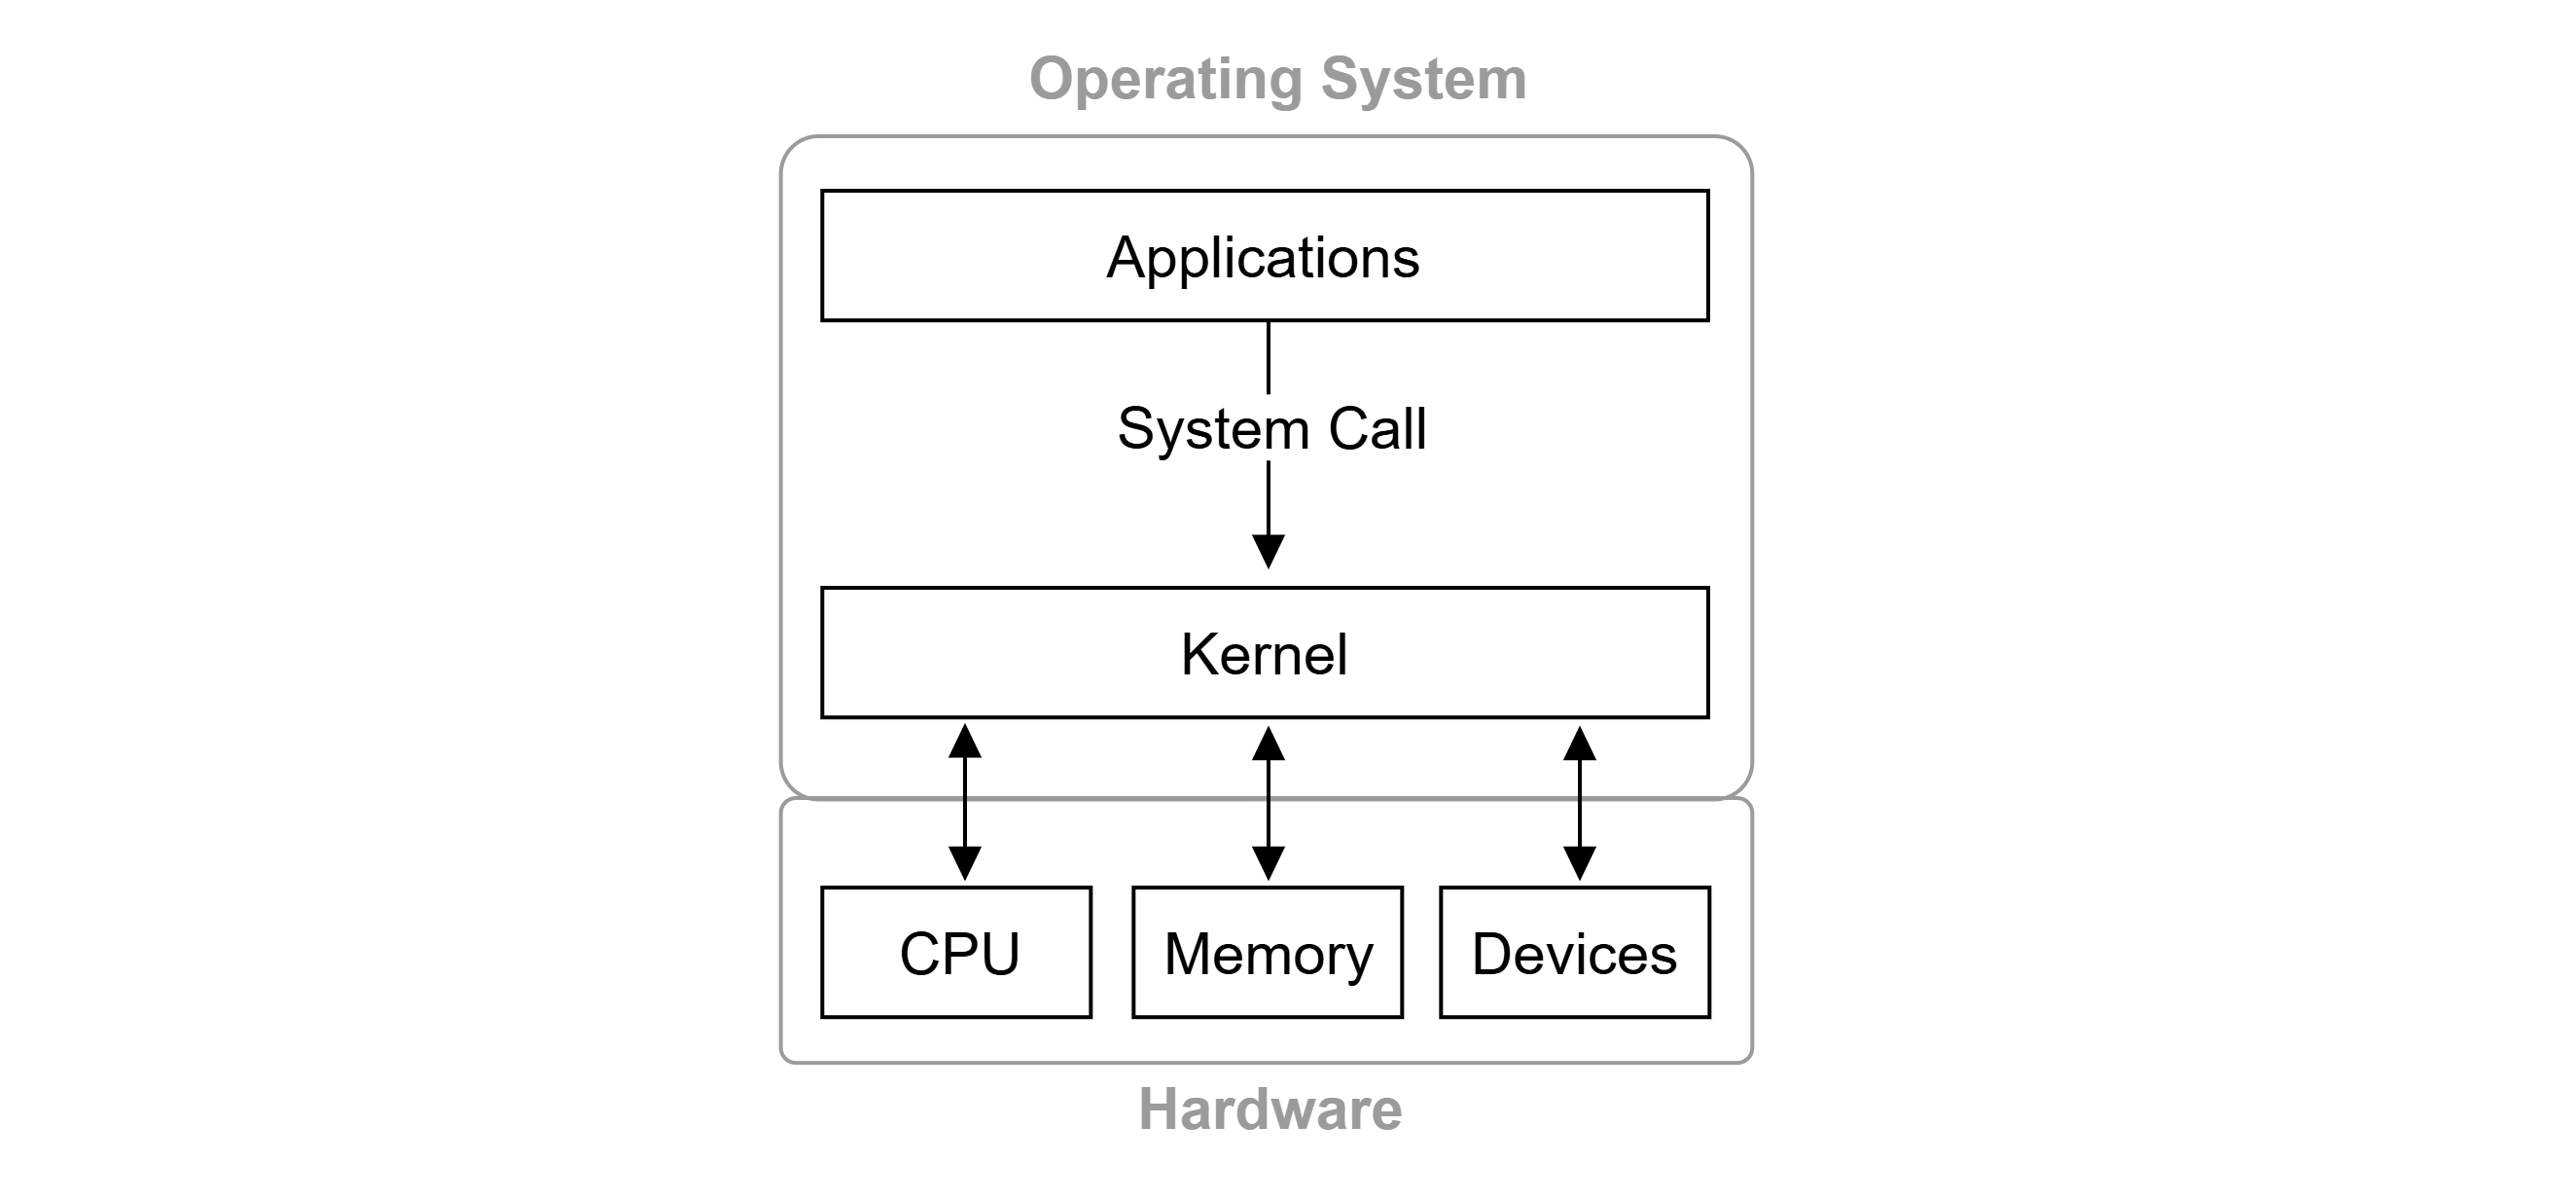
\includegraphics[width=\textwidth]{Sections/cpu/kernel.png}
    \caption{User-level applications make syscalls to the kernel to access hardware resources.}
    \label{fig:kernel}
\end{figure}

\newpage

\begin{Def}[Bus]

    A \textbf{bus} is a collection of physical signal lines (wires or pins) and protocols that carry data, addresses, and control signals between 
    components inside a computer (e.g.\ CPU, memory, I/O devices) or between multiple boards and peripherals. There are two main types of buses:
    \begin{itemize}
        \item \textbf{Serial Bus:} Transfers data one bit at a time over a single channel (e.g., USB).
        \item \textbf{Parallel Bus:} Transfers multiple bits simultaneously over multiple channels (e.g., PCI).
    \end{itemize}
\end{Def}

\begin{Def}[Device Drivers]

  The kernel exposes generic interfaces to various sub-systems (e.g., file system) that user processes can use to perform tasks; \textbf{Device drivers} implement such interfaces,
  translating generic system calls into hardware-specific operations for specific devices (e.g., disk drives, network cards, etc.). Drivers must be loaded into kernel space.
\end{Def}

\noindent
This text does not concern assembly code, so \underline{\textbf{do not}} get caught in the specifics of this Example: 
\begin{Example}[Assembly Code]

    \label{ex:assembly_code}
    An assembly example demonstrating initialized (.data) and uninitialized (.bss) data sections:

    \begin{lstlisting}[language={[x86masm]Assembler}, numbers=none]
    section .data               ; Initialized data section
        num1    dd  7           ; num1 is initialized to 7
        num2    dd  3           ; num2 is initialized to 3

    section .bss                ; Uninitialized data section
        temp    resd 1          ; temp is reserved (uninitialized)
        result  resd 1          ; result is reserved (uninitialized)

    section .text               ; Code section
        global _start

    _start:
        mov eax, [num1]         ; Load num1 into eax
        mov [temp], eax         ; Store num1 in temp
        mov ebx, [num2]         ; Load num2 into ebx
        add eax, ebx            ; Add num2 to eax (eax = num1 + num2)
        mov [result], eax       ; Store the sum in result
    ; Exit syscall removed for simplicity
    \end{lstlisting}

    \noindent
    In this example, `num1' and `num2' are initialized before execution, while `temp' and `result' are uninitialized and only receive values during program execution.
\end{Example}

\newpage 
\section{Code Security}

At a \emph{very} high-level, vulnerabilities exploited by hackers stem from flaws that the programmer forgot to consider (i.e., bugs).
To learn more on cybersecurity, consider our other text \underline{\href{https://github.com/Concise-Works/Cyber-Security/blob/main/main.pdf}{here}}.

\begin{Def}[Proper Encapsulation]

    \label{def:proper_encapsulation}

    \textbf{Proper encapsulation} is the practice of hiding implementation details and exposing only necessary interfaces to prevent unauthorized access or modification.
\end{Def}
\begin{Example}[Student Class]

    \label{ex:student_class}

    Consider a simple `Student' class in an object-oriented programming language:

    \begin{lstlisting}[language=Java, numbers=none]
    public class Student {
        private String name; // Private field, not accessible outside the class
        private int age;     // Private field, not accessible outside the class

        public Student(String name, int age) {
            this.name = name;
            this.age = age;
        }

        public String getName() { // Public method to access name
            return name;
        }
        // Other methods...
    }
    \end{lstlisting}
    Upon creating a new student instance \texttt{new Student("Alice", 20)}, the name and age are private, preventing direct access via \textbf{dot notation} (e.g., \texttt{student.name}).
    The only way to access the name is through the public method \texttt{getName()}. Here we do not have a method for accessing age.
\end{Example}

\begin{Def}[Risks of Accessing Main Memory]

    \label{def:accessing_main_memory}

    Programs accesses main memory (RAM) to read and write data; \textbf{It's critical} that 
    such \underline{references to RAM are abstracted} to avoid malicious or accidental access of data.

    For example, in Java when users print objects, instead of 
    printing the object's memory address, it prints the \texttt{toString()} method, which \textbf{by default} prints the class name and hash code of the object.
\end{Def}
\noindent
In conclusion, there are significant risks when dealing with memory management.
% 
\newpage 

\section{Stack Data Structures}
\label{sec:stacks_heaps}

\noindent
Let's talk about our first data structure, the stack:
\begin{Def}[Stack]

    A \textbf{stack data structure} is a collection of elements that follows a \textbf{Last In, First Out} (LIFO) principle. I.e., in a 
    stack of plates, the last added plate is the first one to be removed, not the middle or bottom/first plate.
    Each \textit{plate} in the stack is called a \textbf{stack frame}.\\

    \noindent
    A \textbf{call stack} is a stack which keeps track of function calls in a program as well as any local variables within such functions.
    
    \underline{This is why we say a variable is in \textbf{scope}}, as when a function is taken off the stack, or a new stack frame 
    is placed on top, the variables in the previous or discarded stack frame are \textbf{no longer accessible}.
\end{Def}

\vspace{-1.5em}

\begin{figure}[ht!]
    \centering
    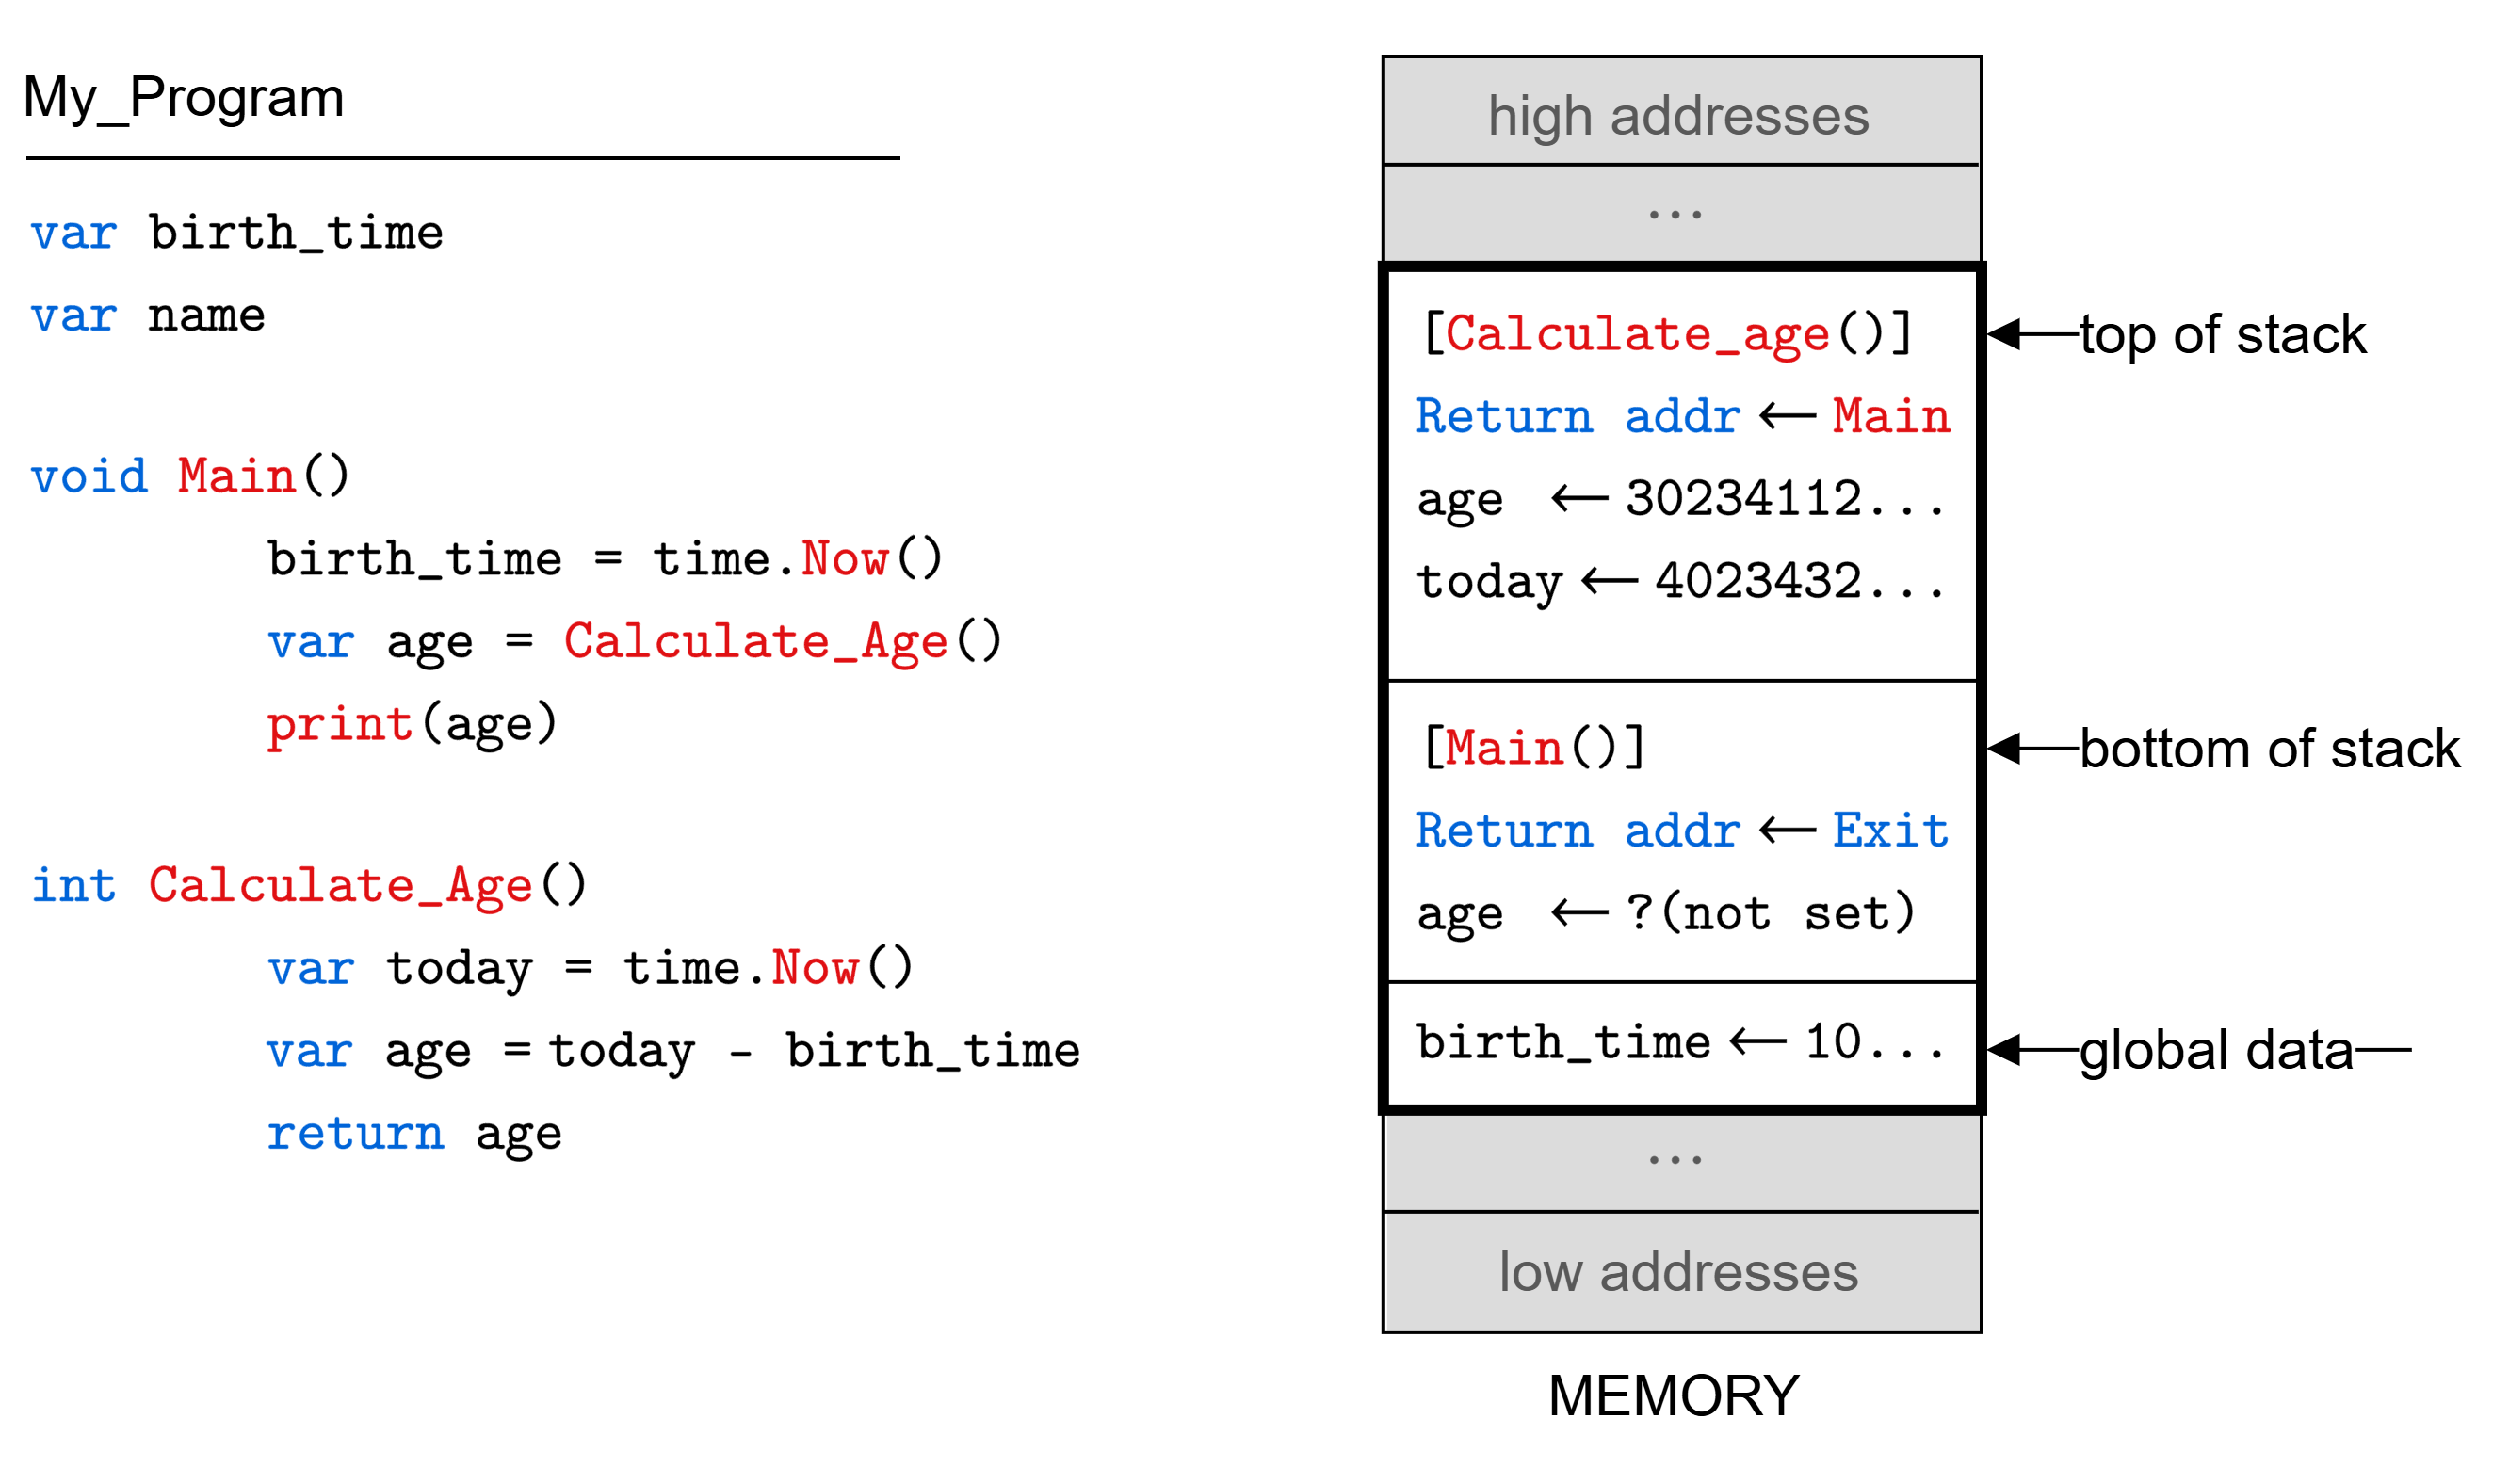
\includegraphics[width=0.8\textwidth]{./Sections/stacks_heaps/call_stack.png}
    \caption{Here is a simplified look at how memory manages the stack. On the left is our program written 
    in some abstract language, and on the right is the call stack in memory (simplified). 
    The program has a global `birth\_time' variable, which is initialized in the \texttt{Main} function. The \texttt{Main} function
    then calls the \texttt{Calculate\_Age} function which uses the `birth\_time' variable to calculate the `age' via the difference of 
    the current time and the `birth\_time.'
    Looking at the memory, we see at the bottom of our memory contains global variables accessible to any frame. Next, is the bottom of the stack, containing a return address to exit 
    the program, while awaiting the result of the function call for `age'. The top of our stack contains another frame that we will return the value
    a new `age' (not the same as the one before) not accessible from the main function. This new frame also contains a new local variable `today.'
    Once this function returns, \texttt{Main} will have the result of its local variable `age.'. Concretely, the 
    `age' variable in both the \texttt{Main} and \texttt{Calculate\_Age} function are completely separate despite sharing the same \textit{name}.}
    \label{fig:call_stack}
\end{figure}

\newpage 

\noindent
\underline{\textbf{Please Note:} The above figure is a simplified version}; This presentation derivatives from what actually happens
for teaching sake. In the following pages we define the stack frame in more detail.

\begin{Tip}
A lot of demonstrations (including this text) will show the stack growing \textbf{upwards}; This is strictly because it's easier to visualize and does not
accurately portray what a stack really does or looks like. In the following pages we will clear this up, and show how the stack actually grows from top-to-bottom.
Of course, there is always room for deviation if a developer wishes to implement a stack in some other arbitrary way. Nonetheless, the following is what one 
might typically expect in a stack implementation.
\end{Tip}

\begin{Def}[Stack Frame Anatomy]

Under the x86-32 calling convention Two registers keep track our place in the stack:
\begin{itemize}
  \item \textbf{Base Pointer (BP/EBP):} Points to the base (i.e.\ ``bottom'') of the current function's stack frame.
  \item \textbf{Stack Pointer (SP/ESP):} Points to the ``top'' of the current function's stack frame, i.e., the next free byte where a push would land.
\end{itemize}

\noindent
When the program starts, the operating system \emph{reserves} a contiguous region of memory for the stack. By convention, the \emph{bottom} of that region lies at a higher address, 
and the stack ``grows downward'' toward lower addresses as data is pushed. If the stack pointer ever moves past the reserved limit---a \textbf{stack overflow} occurs.
\\

\noindent
A single \textbf{stack frame} itself is a contiguous block of memory in which the function stores:
\begin{itemize}
  \item \textbf{Parameters:} The arguments passed in by the caller,  
  \item \textbf{Return Address:} The address of the next instruction to execute after the function returns,
  \item \textbf{Old Base Pointer:} The caller's `EBP', saved so that on return we can restore the previous frame,
  \item \textbf{Local Variables:} Space for any locals or temporaries that the function needs.  
\end{itemize}

\noindent
This is why variables in previous or new functions calls become ``\textbf{out of scope}'' (no longer accessible), as they belong to some other stack frame; 
When it comes to \textbf{Global Variables}, they live in a separate region of memory, defined by the \textbf{data segment} (\ref{def:machine_code}).

Moreover, a call to a new function invokes the \underline{\textbf{call} instruction}, this automatically pushes the return address to the current frame onto the stack.
Additionally, the CPU reserves the \textbf{EAX} register for the return value (number or address) of a function. 
When the function returns, it can place its result in `EAX', and the caller can retrieve it from there. During constant use 
the `EAX' \underline{register may contain \textbf{garbage}} data from previous use, unless explicitly set to zero or some other value.
\end{Def}

\newpage 

\begin{table}[h]
\centering
\resizebox{\textwidth}{!}{
\begin{tabular}{|c|c|l|}
\hline
\multicolumn{3}{|c|}{\textbf{High Addresses}} \\ \hline
\textbf{Contents}       & \textbf{Offset} & \textbf{Notes} \\
\hline
\emph{(Parameters 3, 4, \(\dots\))} & \(\mathit{EBP} + 16\), \(+20\), \(\dots\) & Third-and-onward arguments, if any. \\ 
Parameter 2            & \(\mathit{EBP} + 12\) & Second argument passed on stack. \\
Parameter 1            & \(\mathit{EBP} + 8\)  & First argument passed on stack. \\
Return Address         & \(\mathit{EBP} + 4\)  & Auto-pushed by the \texttt{call} instruction.\\
Old EBP (Saved BP)     & \(\mathit{EBP} + 0\)  & The caller's base pointer \\
\hline
\multicolumn{3}{|c|}{\textbf{Current Frame (locals/temporaries)}} \\ \hline
Local Variable 1        & \(\mathit{EBP} - 4\)  & First 4-byte local (or smallest slot). \\
Local Variable 2        & \(\mathit{EBP} - 8\)  & Next 4-byte local or part of a larger object. \\
\(\dots\)                      & \( \vdots \)         &(additional locals at \(\mathit{EBP} - 12,\ -16,\ \dots\)) \\
\hline
\multicolumn{3}{|c|}{\textbf{Low Addresses}} \\ \hline
\end{tabular}
}
\caption{Typical x86-32 Stack-Frame Layout, where offsets are typically a multiple of 4 bytes.}
\end{table}

\begin{figure}[!ht]
    \centering
    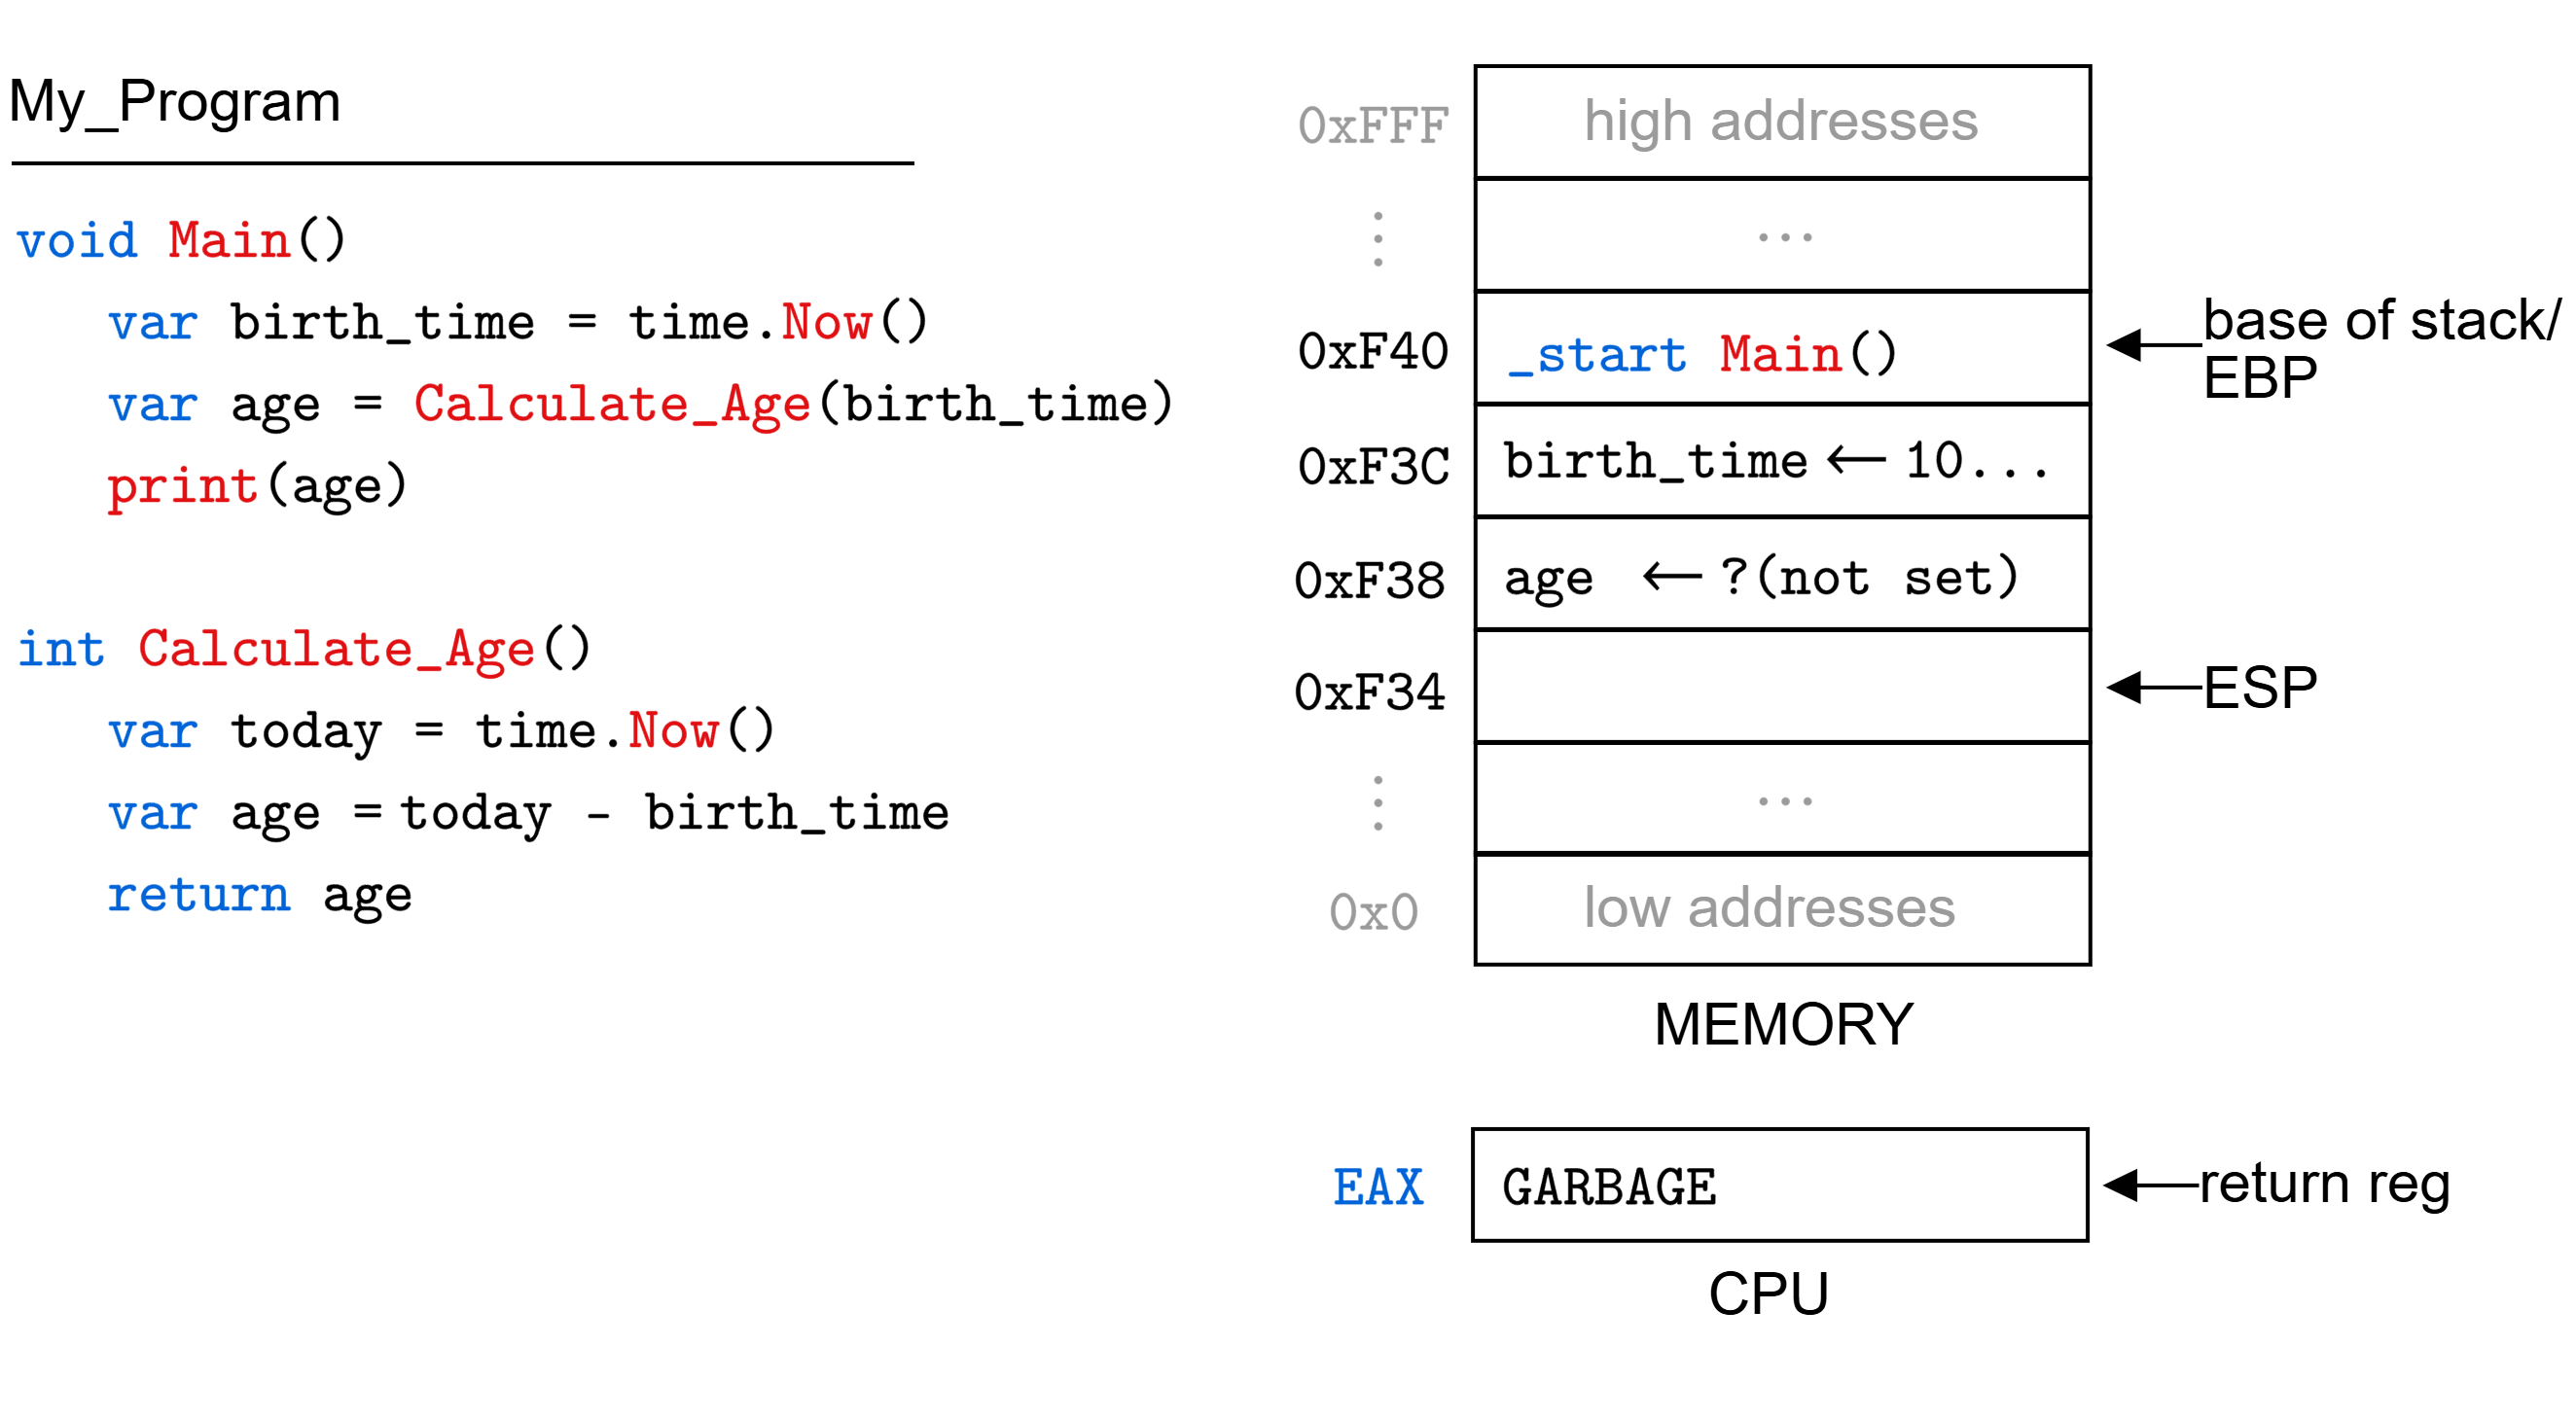
\includegraphics[width=\textwidth]{./Sections/stacks_heaps/call_stack_precise.png}
    \caption{Revisiting Figure (\ref{fig:call_stack}) with slight alterations to the code: This is a snapshot of the code executing right before \texttt{CalculateAge(birth\_time)} is called. For simplicity sake,
    let's say the stack begins at address \texttt{0xF40} (Hexadecimal), growing downwards. Here the base of the stack and the EBP are one and the same.
    We include the CPU's EAX (return register), which contains garbage. Address \texttt{0xF38} is currently just reserved space for `age'.}

\label{fig:call_stack_precise}
\end{figure}

\newpage 

\begin{figure}[!ht]
    \centering
    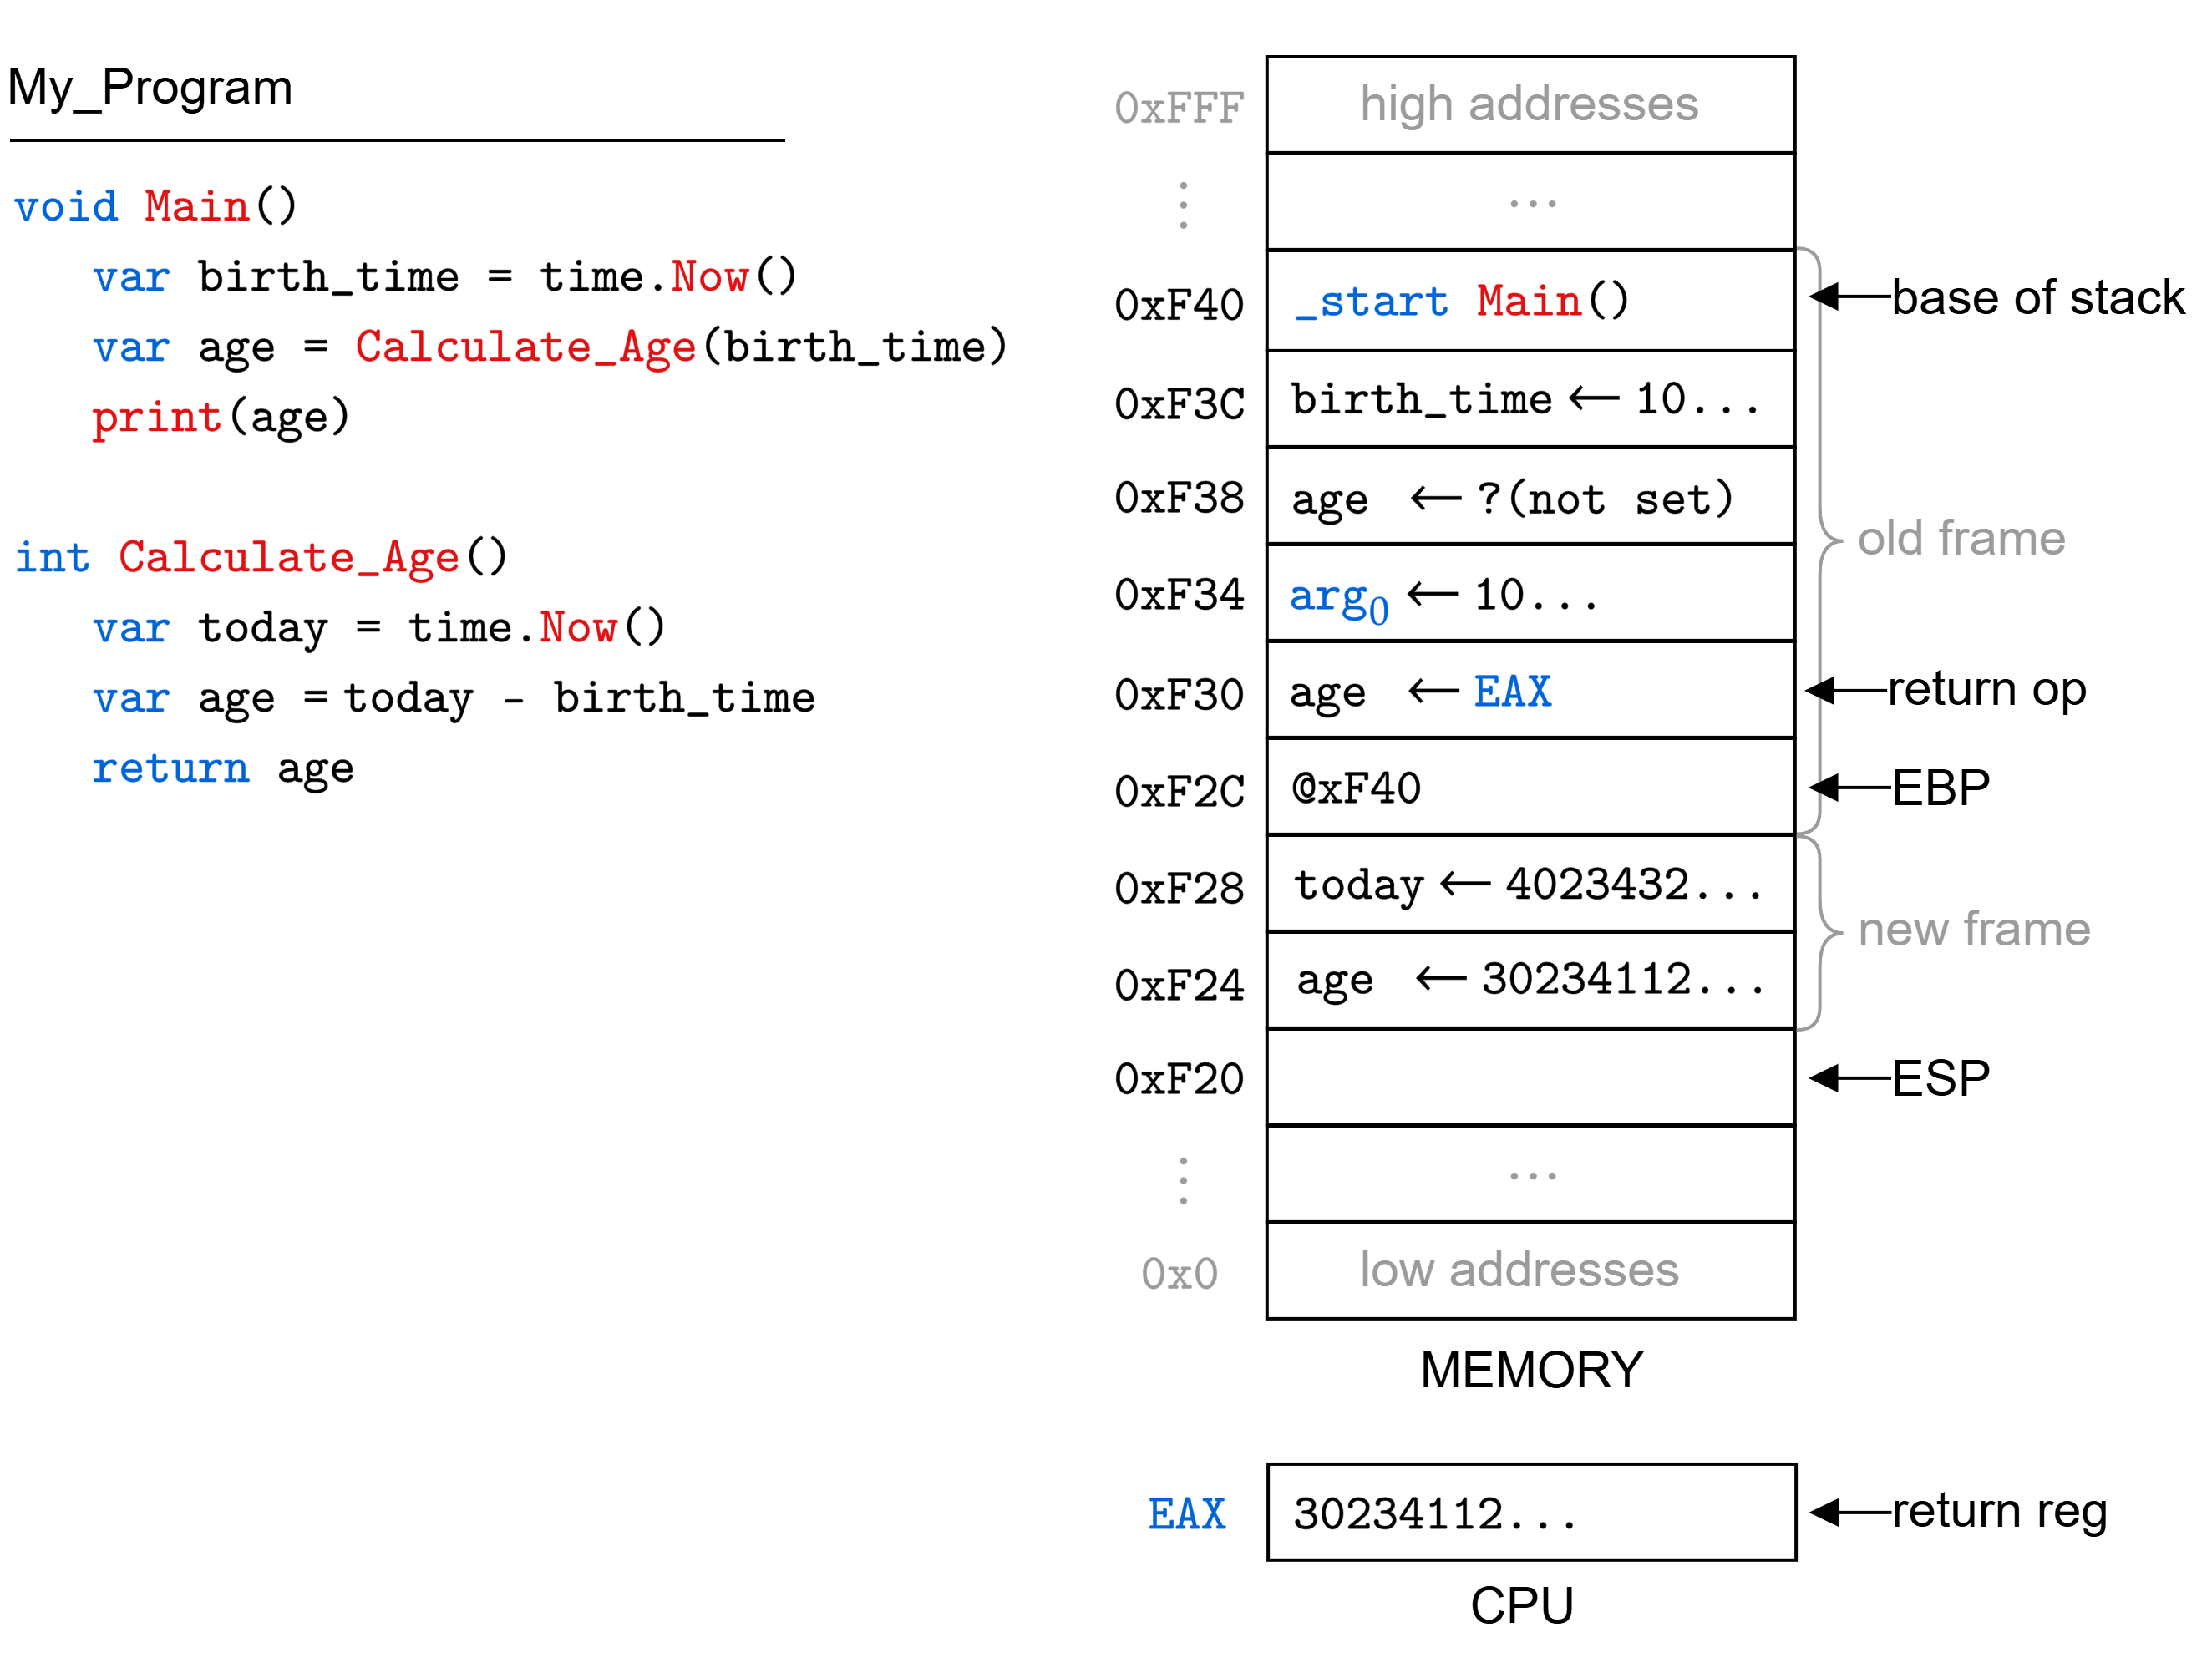
\includegraphics[width=\textwidth]{./Sections/stacks_heaps/call_stack_after.png}
    \caption{Revisiting Figure (\ref{fig:call_stack_precise}) at the moment the function \texttt{CalculateAge(birth\_time)} has supplied its return value to the EAX register, and is about to return.
    We see that before calling \texttt{CalculateAge(birth\_time)}: The old frame pushed it's arguments (\texttt{birth\_time}) onto the stack, then the return address (IP/Next Instruction) onto the stack,
    and finally the old EBP (Base Pointer) onto the stack. The `new frame' then sets the saved EBP address to the current EBP, concluding the old frame into the `new frame'. Moreover, since the offset
    looks for local variables below \texttt{0xF40}, the above `birth\_time' and `age' are \textbf{out of scope} for the `new frame', vice-versa. \textbf{Note:} This is 
    still a high-level abstraction of what actually happens sequentially with opcodes; Nonetheless, this is the fundamental idea of how a stack works. }
    \label{fig:call_stack_after}
\end{figure}

\noindent 
This concludes our discussion on stack structures; We continue with the heap structure next.

\newpage 

\noindent
\section{Heap Data Structures}
\label{sec:heap}

\noindent
So far we have simply said global data is declared in the \textbf{data segment} of memory. There is a second segment 
of memory that builds ontop of this called the \textbf{heap}:
\begin{Def}[Heap -- Dynamic vs. Static Memory]

    When a program runs there is a \textbf{static} (fixed) region reserved for the program's data segment (local/global variables). 
    During execution, more objects may be created, needing additional memory; A new region of memory is reserved \textbf{dynamically},
    building upwards from the top of the data segment, \underline{called the \textbf{heap}}.\\
    
    \noindent
    Language protocols either \textbf{manually} (e.g., Assembly, C) or \textbf{automatically} (e.g., Python, Java) manage this memory:
    \begin{itemize}
        \item \textbf{Manual Memory Management:} The programmer must explicitly allocate and deallocate memory using functions like `malloc' and `free' in C.
        \item \textbf{Automatic Memory Management:} The language runtime automatically allocates and deallocates memory, often using a \textbf{garbage collector} to reclaim unused memory (no variables pointing to it).
\end{itemize}

\noindent
Unlike the stack, this allows values to be accessed from anywhere in the program, regardless of the function call or scope.
\end{Def}

\noindent
To continue we must understand what a hash table is, and how arrays and objects work in memory:
\begin{Def}[Hash Table]

    \label{def:hash_table}

    A \textbf{hash table} is a data structure that maps keys to values, allowing for efficient retrieval of values based on their keys.
    It uses a \textbf{hash function}, which takes a key (e.g. a number or string) as input and produces a fixed-size (i.e., output modulo the table size) hash value for the index.

    \textbf{Note:} The input in many context (typically cryptographic), may be called `data' or `message'; The output: hash, checksum, fingerprint, or digest.
\end{Def}
\begin{Def}[Arrays in Memory]

    In memory array elements are stored sequentially. A reference to 
    an array is a pointer to the first element. To terminate reading an array, we must either know the size of said 
    array or have some sentinel value (e.g., `null' or `0') to indicate the end of the array.\\
    
    \noindent
    E.g., An array of 3 integers (4 bytes each) occupying [0xF00-0xF0C]: $[1,2,3,\texttt{null}]$.
\end{Def}
\newpage 

\noindent
Objects behave very similarly to arrays, but with a few key differences:
\begin{Def}[Objects in Memory]

    An \textbf{Object} (or \textbf{struct}), is a collection of key-value pairs, 
    where each key is called a \textbf{field} or \textbf{attribute} and each value can be any data type (e.g., number, string, or address).

    Attributes are stored in array like fashion, where each element is a fixed-offset from the head (start) of the object.
    The object itself is a pointer to the first element. Accessing attributes works differently in compiled (e.g., C) vs. interpreted (e.g., Python) languages:
    \begin{itemize}
        \item \textbf{Compiled Languages:} There is no lookup, as the compiler has \emph{hardcoded} the offsets of each attribute interaction (e.g., `object.attribute' is translated to a direct memory access).
        \item \textbf{Interpreted Languages:} The interpreter looks up a hash table lookup for the attribute name.
    \end{itemize}

    \noindent
    Depending on the use case, objects may be stored in the heap or stack:
    \begin{itemize}
        \item \textbf{Static Objects:} An objects whose size is known at compile time can be allocated on the stack. I.e., no changes 
        to the object are made after creation (e.g., Math and Time objects, which purely exist to compute).
        \item \textbf{Dynamic Objects:} Often just called \textbf{objects}, are allocated on the heap, allowing for dynamic resizing and modification (e.g.,
        a student object with attributes like `name', `age', and `grades' that can change over time).
    \end{itemize}

\end{Def}

\noindent 
We define the following for completeness sake:
\begin{Def}[Classes \& Interfaces]

    Object-oriented programming is a paradigm where objects are the main building blocks of the program.
    A \textbf{class} is a blueprint for defining how an object will behave once \textbf{instantiated} (created). In this paradigm,
    functions are called \textbf{methods}, as they are defined and used within the class (i.e., globally does not exist in independence).\\

    \noindent
    Some languages (e.g., Java, C++) support \textbf{interfaces} (or protocols), which specify a set of methods that implementing classes must provide. Although the terminology varies 
    (abstract classes, traits, protocols, etc.), they all ultimately describe capabilities an object must fulfill.
\end{Def}


\begin{Tip}
    Often when trying to print an object in Java we see \texttt{ClassName@HEX}, 
    where \texttt{HEX} is the object's identity hash code instead of the memory address; Memory access poses security risks to memory
    manipulation.
\end{Tip}

\newpage 

\noindent
Strings are not what they seem:
\begin{Def}[Strings \& Characters in Memory]

    \noindent
    A \textbf{character} is represented by a numeric code unit:
    \begin{itemize}
      \item In C, a single \texttt{char} (1 byte) typically holds an ASCII code (0--127).
      \item In Java, \texttt{char} is a 16-bit UTF-16 code unit (U+0000..U+FFFF). ASCII values (0--127) map directly to the same Unicode code points, so:
      \begin{verbatim}
        char c = `A';
        System.out.println((int)c);  // prints 65, since `A' is U+0041
      \end{verbatim}
      
      \vspace{-1.5em}
      \noindent
      Characters beyond U+FFFF use two \texttt{char} values (a surrogate pair). This allows us to do things like checking for 
      valid characters:
      \begin{verbatim}
        if ((c >= `a' && c <= `z') || (c >= `A' && c <= `Z')) {
            // c is in `a'..`z' or `A'..`Z'
        }
    \end{verbatim}

    \vspace{-1.5em}
    \noindent
    We can also perform arithmetic on \texttt{char}:
    \begin{verbatim}
    char c = 'A';        // U+0041 (65)
    char next = (char)(c + 1);  // 'B' (66)
    \end{verbatim}
    \end{itemize}
    
    \vspace{-1.5em}
    \noindent
    \rule{\textwidth}{0.4pt}\\ 

    \noindent
    \underline{Typically, a \textbf{string} is stored as a contiguous array of \textbf{characters}.} In low-level languages (e.g.\ C),
    that array ends with a null terminator (\verb|\0|) and literal strings reside in the data segment. 
    In higher-level languages (e.g.\ Java, Python), strings are full objects with methods. For e.g.,\\

    \noindent
    \textbf{C:}  
    \begin{itemize}
      \item String literals (e.g.\ \texttt{"Hello"}) are placed in the (often read-only) data segment.
      \item Runtime-constructed strings (via \texttt{malloc}, \texttt{strcpy}, etc.) live on the heap.
    \end{itemize}

    \noindent
    \textbf{Java:}  
    \begin{itemize}
      \item Compile-time literals are \textbf{interned} (stored as a single shared copy) into the \textbf{String Constant Pool} section (specially reserved on the heap).  
      \item Any other \texttt{String} (e.g.\ via \texttt{new String(...)}, concatenation, or user input) also resides on the heap but outside the pool.  
      \item Because Java strings are immutable, interning lets multiple references share the same character data.
    \end{itemize}

    
\end{Def}

\newpage

\noindent
With slight alterations to our code in Figure (\ref{fig:call_stack_after}), we illustrate heaps and arrays:

\begin{figure}[!ht]
    \centering
    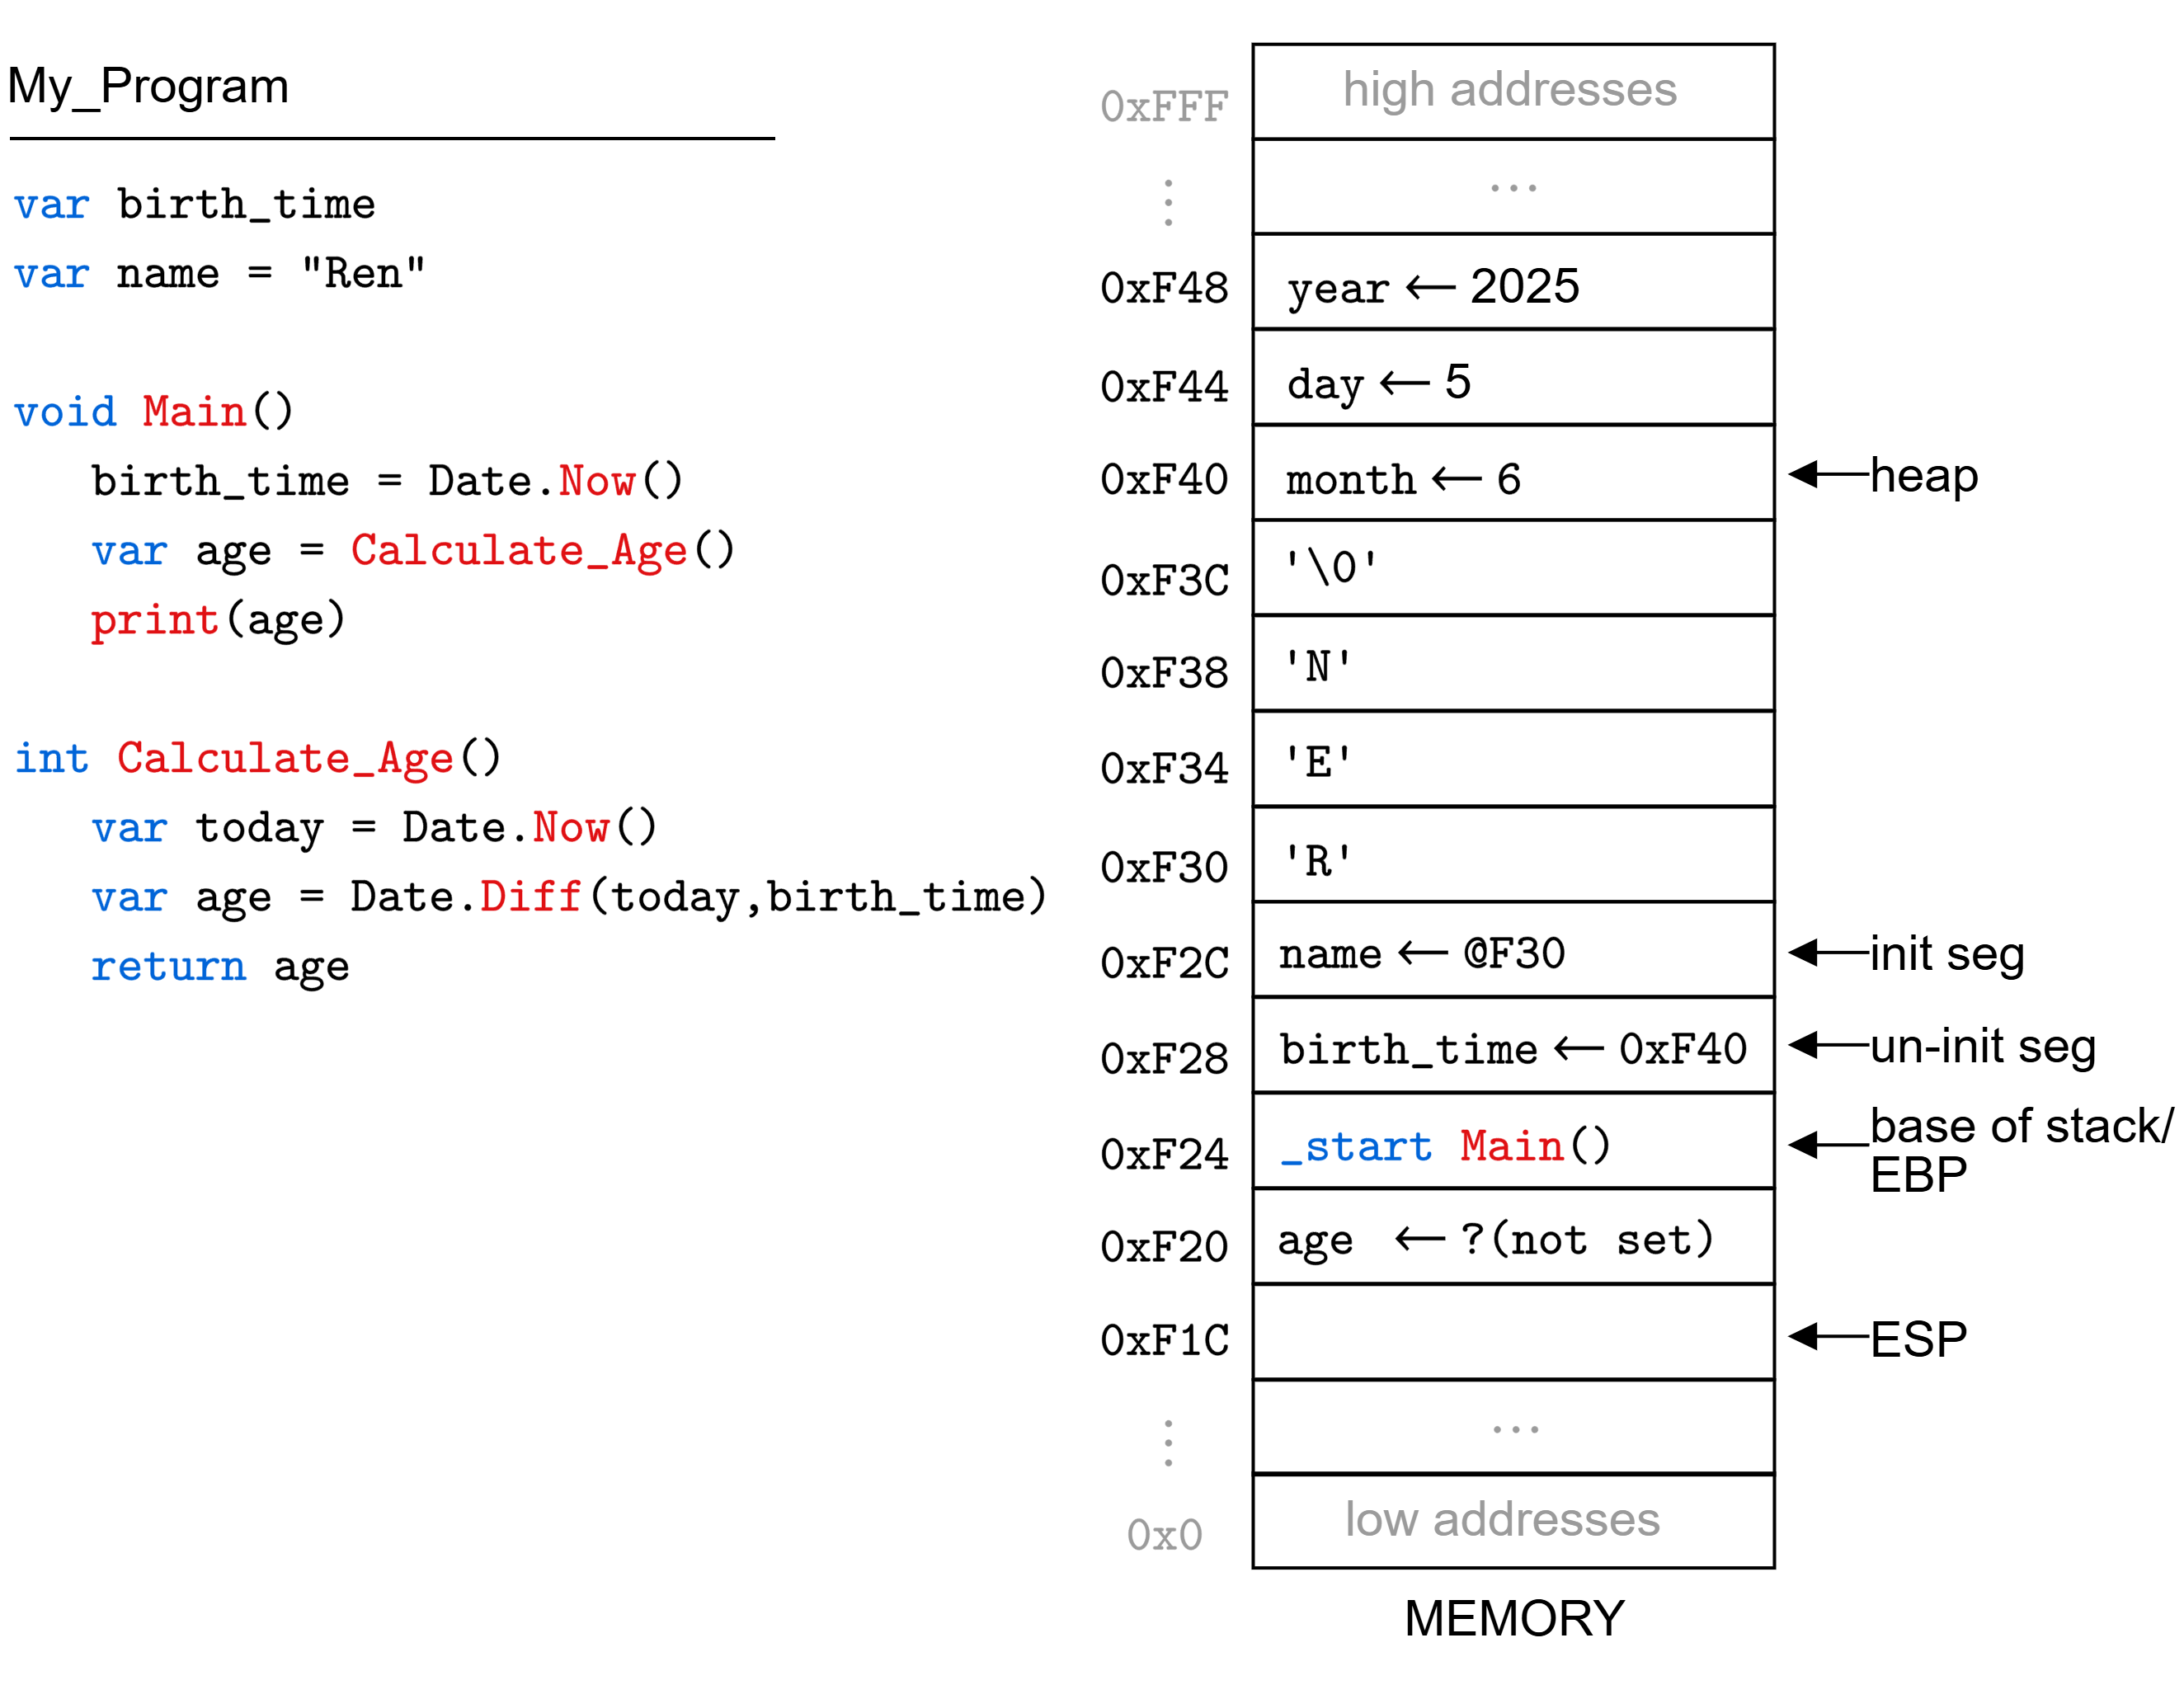
\includegraphics[width=\textwidth]{./Sections/stacks_heaps/heap_array.png}
    \caption{Here \texttt{birth\_time} and \texttt{name} are global variables. Following the C convention, \texttt{birth\_time} is placed in the 
    uninitialized data segment, while \texttt{name} is placed in the initialized data segment. Since \texttt{name} is a string, it holds a 
    reference to the first character in the string, which is stored contiguously in the initialized data segment ending with a null terminator (`\texttt{\textbackslash 0}').
    During execution, \texttt{Date.Now()} a method call from a \texttt{Date} object is called; This method returns a new object, which is placed on the heap with 
    its attributes (\texttt{month}, \texttt{day}, \texttt{year}) stored contiguously in memory. \textbf{Note:} Methods such as \texttt{Date.Diff()} are code (not data), 
    which do not live in the heap or stack.}
    \label{fig:heap_array}
\end{figure}

\begin{Def}[Factory Method]

    A \textbf{factory method} is a function that creates and returns an object, often initializing it with default values or parameters.
    In Figure (\ref{fig:heap_array}), the method \texttt{Date.Now()} is a factory method that creates a new \texttt{Date} object with the current date and time.
\end{Def}

\noindent
The below illustration summarizes the heap and stack in memory:
\begin{figure}[!ht]

    \hspace{-6em} 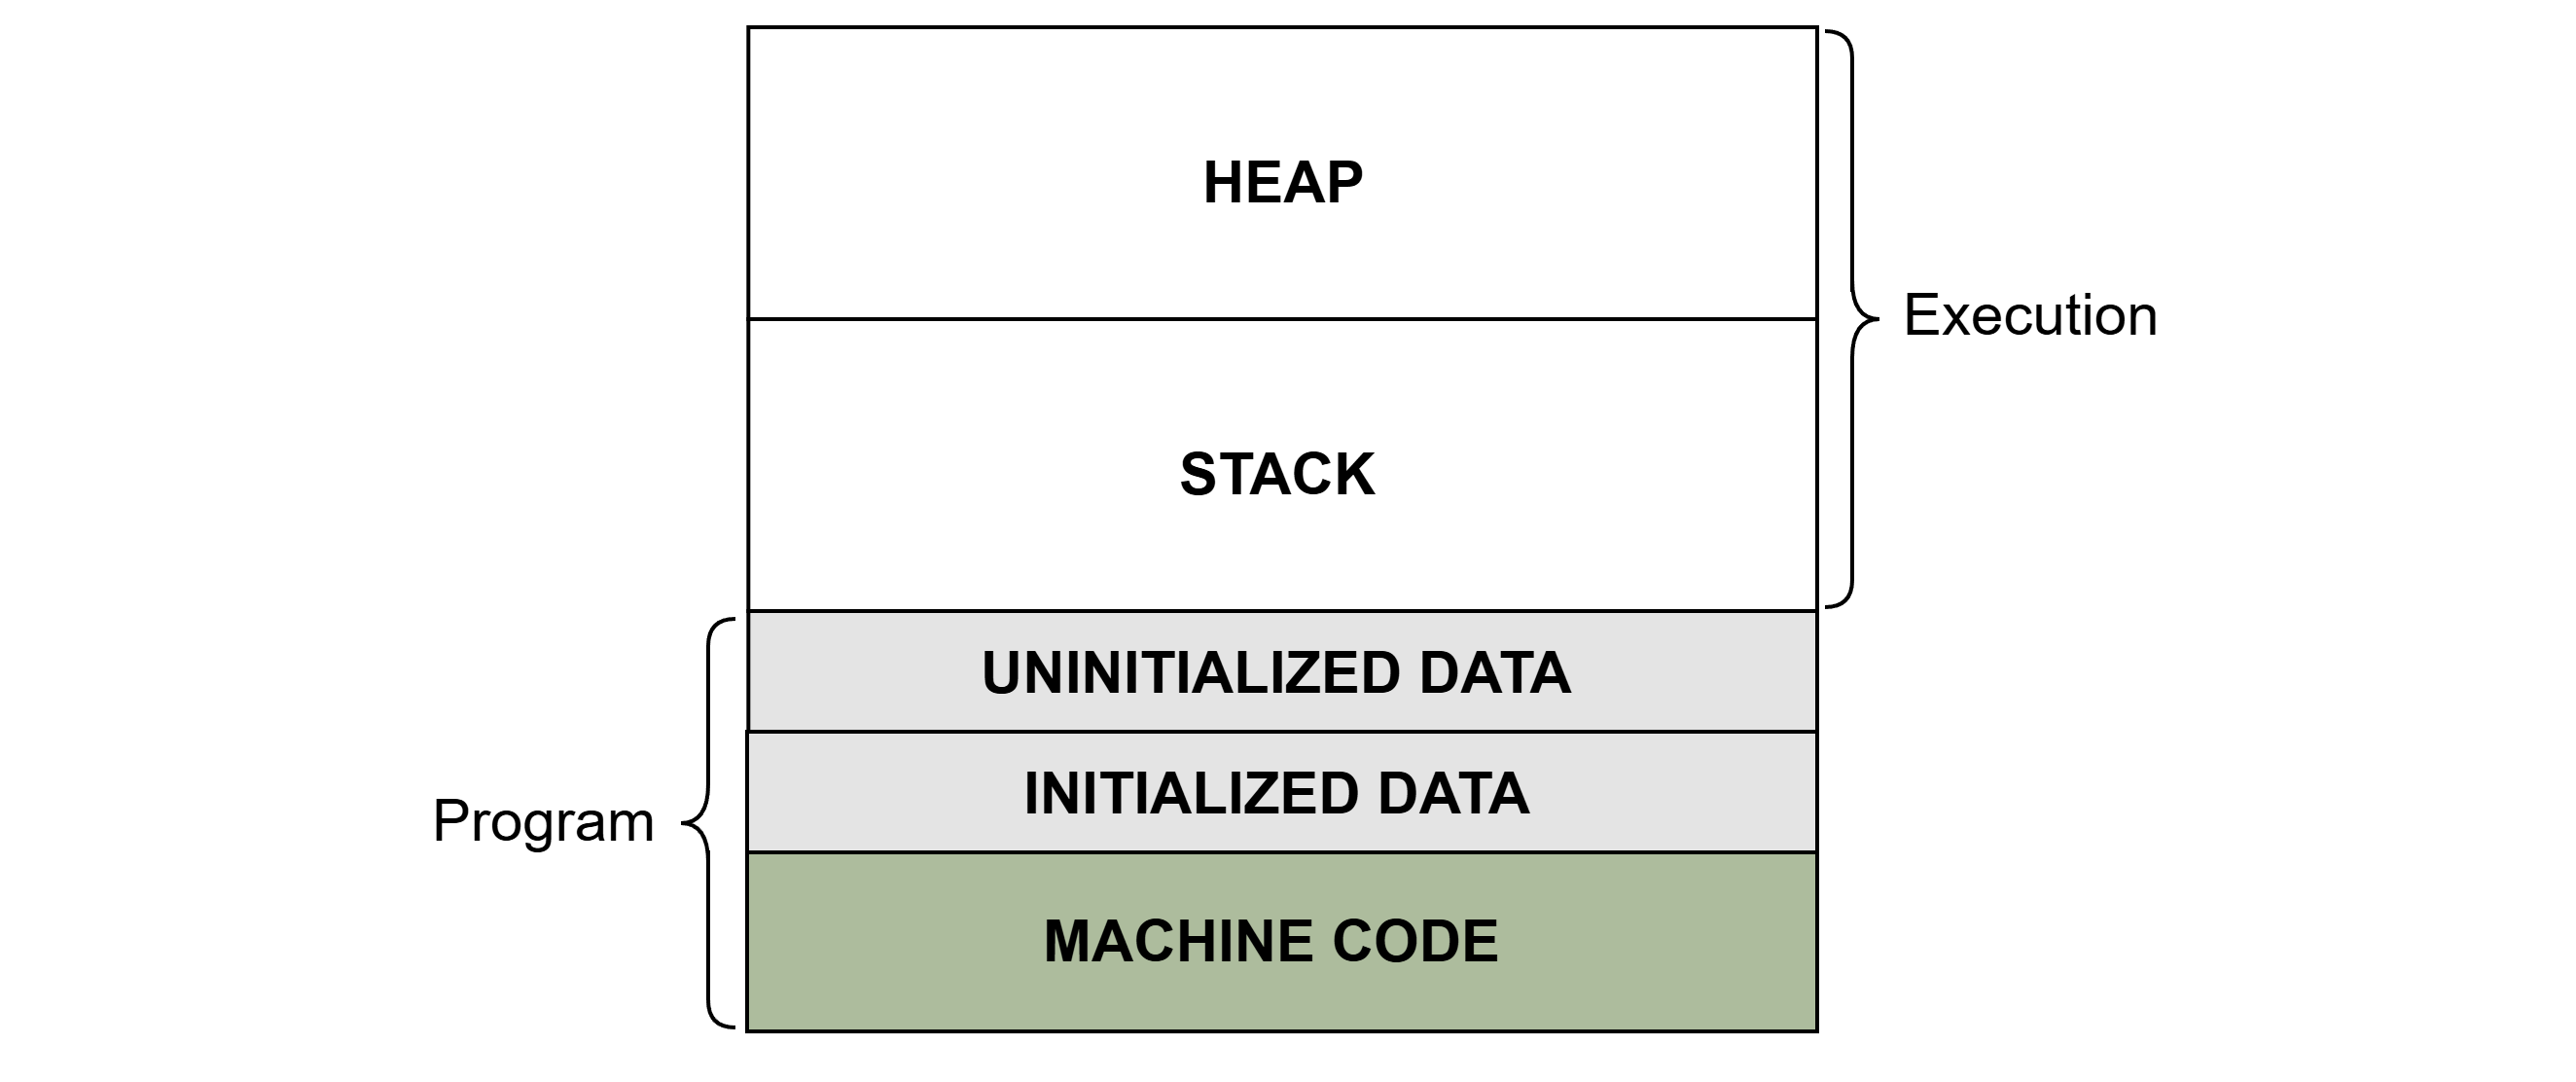
\includegraphics[width=1.3\textwidth]{./Sections/stacks_heaps/stack_heap_memory.png}
    \caption{The above figure demonstrates the relationship from bottom-to-top the order at which data is 
    loaded into memory. First the program compiles to machine code and loaded by the OS into memory.
    From there, provisions to the data segment (static memory: uninitialized and initialized) are made. Depending 
    on the OS, some objects may have already been loaded into the heap, which are referenced by initialized data segment variables.
    Then as functions are called, the stack grows downwards within its allotted memory space. During execution of each stack frame,
    new objects may be placed on the heap, referenced by variables in the stack or data segment. Then depending on the language,
    a garbage collector periodically checks for objects with no references (i.e., no variables pointing to them) and deallocates them;
    Alternatively, the program explicitly deallocates memory using functions like `free' in C.}
    \label{fig:stack_heap_memory}
\end{figure}
% \newpage 

\section{Hashing \& Collisions}

In the previous section we lightly touched on the topic of hashing in Definition (\ref{def:hash_table}). 
This section will dive into more detail and difficulties collisions in hashing.

\begin{Def}[Collisions]

    A \textbf{collision} occurs when two different keys hash to the same index in a hash table.
    This is an unavoidable issue in hashing when keys begin to exceed the available indices.
\end{Def}

\begin{figure}[ht!]

    \centering
    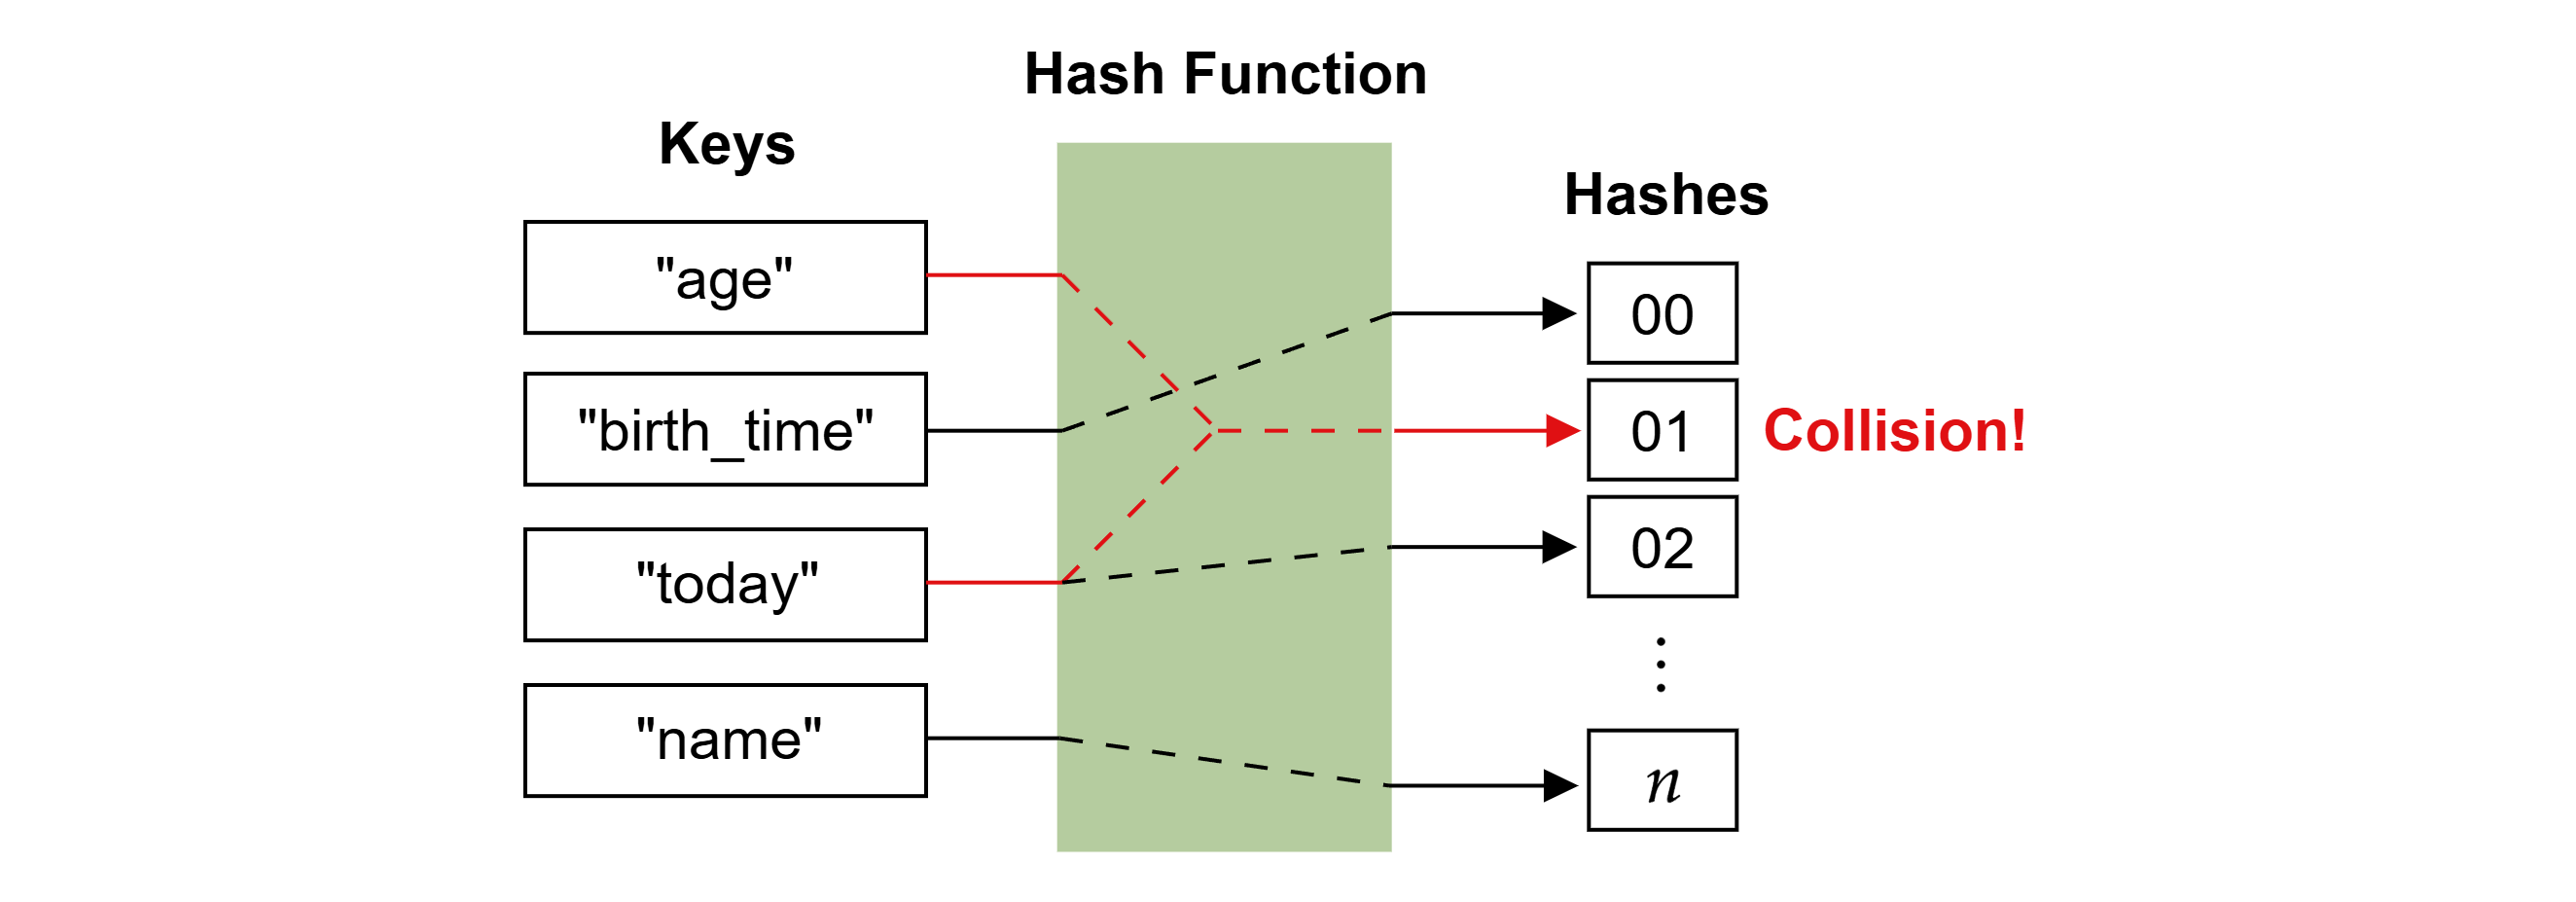
\includegraphics[width=\textwidth]{Sections/hash/collision.png}
    \caption{Four keys (`age', `birth\_time', `today', `name') go through a hash function to $n$ possible indices.
    Keys, `birth\_time' and `name', find a unique one-to-one mapping; However, `age' and `today' both hash to the same index, causing a collision.}
    \label{fig:collision}
\end{figure}
\begin{Example}[Simple Hashing Algorithm]

    Consider the hashing algorithm $H$, it takes the first ASCII value modulo the size 
    of the table. Concretely, $H(k):=\text{ASCII}(k[0])\ \%\ n$, where $n$ is the size of the table.\\

    \noindent
    Given the function $H$, we consider the following keys under a hash table of size $10$:

    \begin{itemize}
        \item \textbf{Key:} `apple' $\rightarrow$ ASCII value $=97$ $\rightarrow$ $H(\text{apple})=97\ \%\ 10 = 7$
        \item \textbf{Key:} `banana' $\rightarrow$ ASCII value $=98$ $\rightarrow$ $H(\text{banana})=98\ \%\ 10 = 8$
        \item \textbf{Key:} `bread' $\rightarrow$ ASCII value $=98$ $\rightarrow$ $H(\text{bread})=98\ \%\ 10 = 8$
    \end{itemize}
    
    \noindent
    Here, we see that `banana' and `bread' both hash to index $8$, causing a collision.
\end{Example}
One could have a superb hashing algorithm, but when space is tight, collisions are inevitable. We'll look at two particular methods for dealing with this issue.

\newpage 

\subsection{Open Addressing}
\noindent
Our first method:
\begin{Def}[Open Addressing]

    \textbf{Open addressing} is a collision resolution method where, upon a collision, the algorithm searches for the next available slot via a probing sequence.\\

    \noindent
    \textbf{Wrap Around:} the algorithm uses a modulo operation (e.g., Given a table size of 10 and request for index 12, the algorithm would use $12\ \%\ 10 = 2$).
    
    \noindent
    \rule{\textwidth}{0.4pt}

    \noindent
    \textbf{Time Complexity:} $O(n)$, where $n$ is the number of elements in the hash table. For example, say the only free index is at 0 with all other
    indices occupied. If we hash to index 1, the algorithm will have to walk all $n$ indices to find the free index at 0. Changing the probe method only switches order of indices checked, not the worst case.\\
    \textbf{Space Complexity:} $O(n)$, where $n$ is the size of the hash table (no additional space).
\end{Def}

\begin{figure}[ht!]

    \centering
    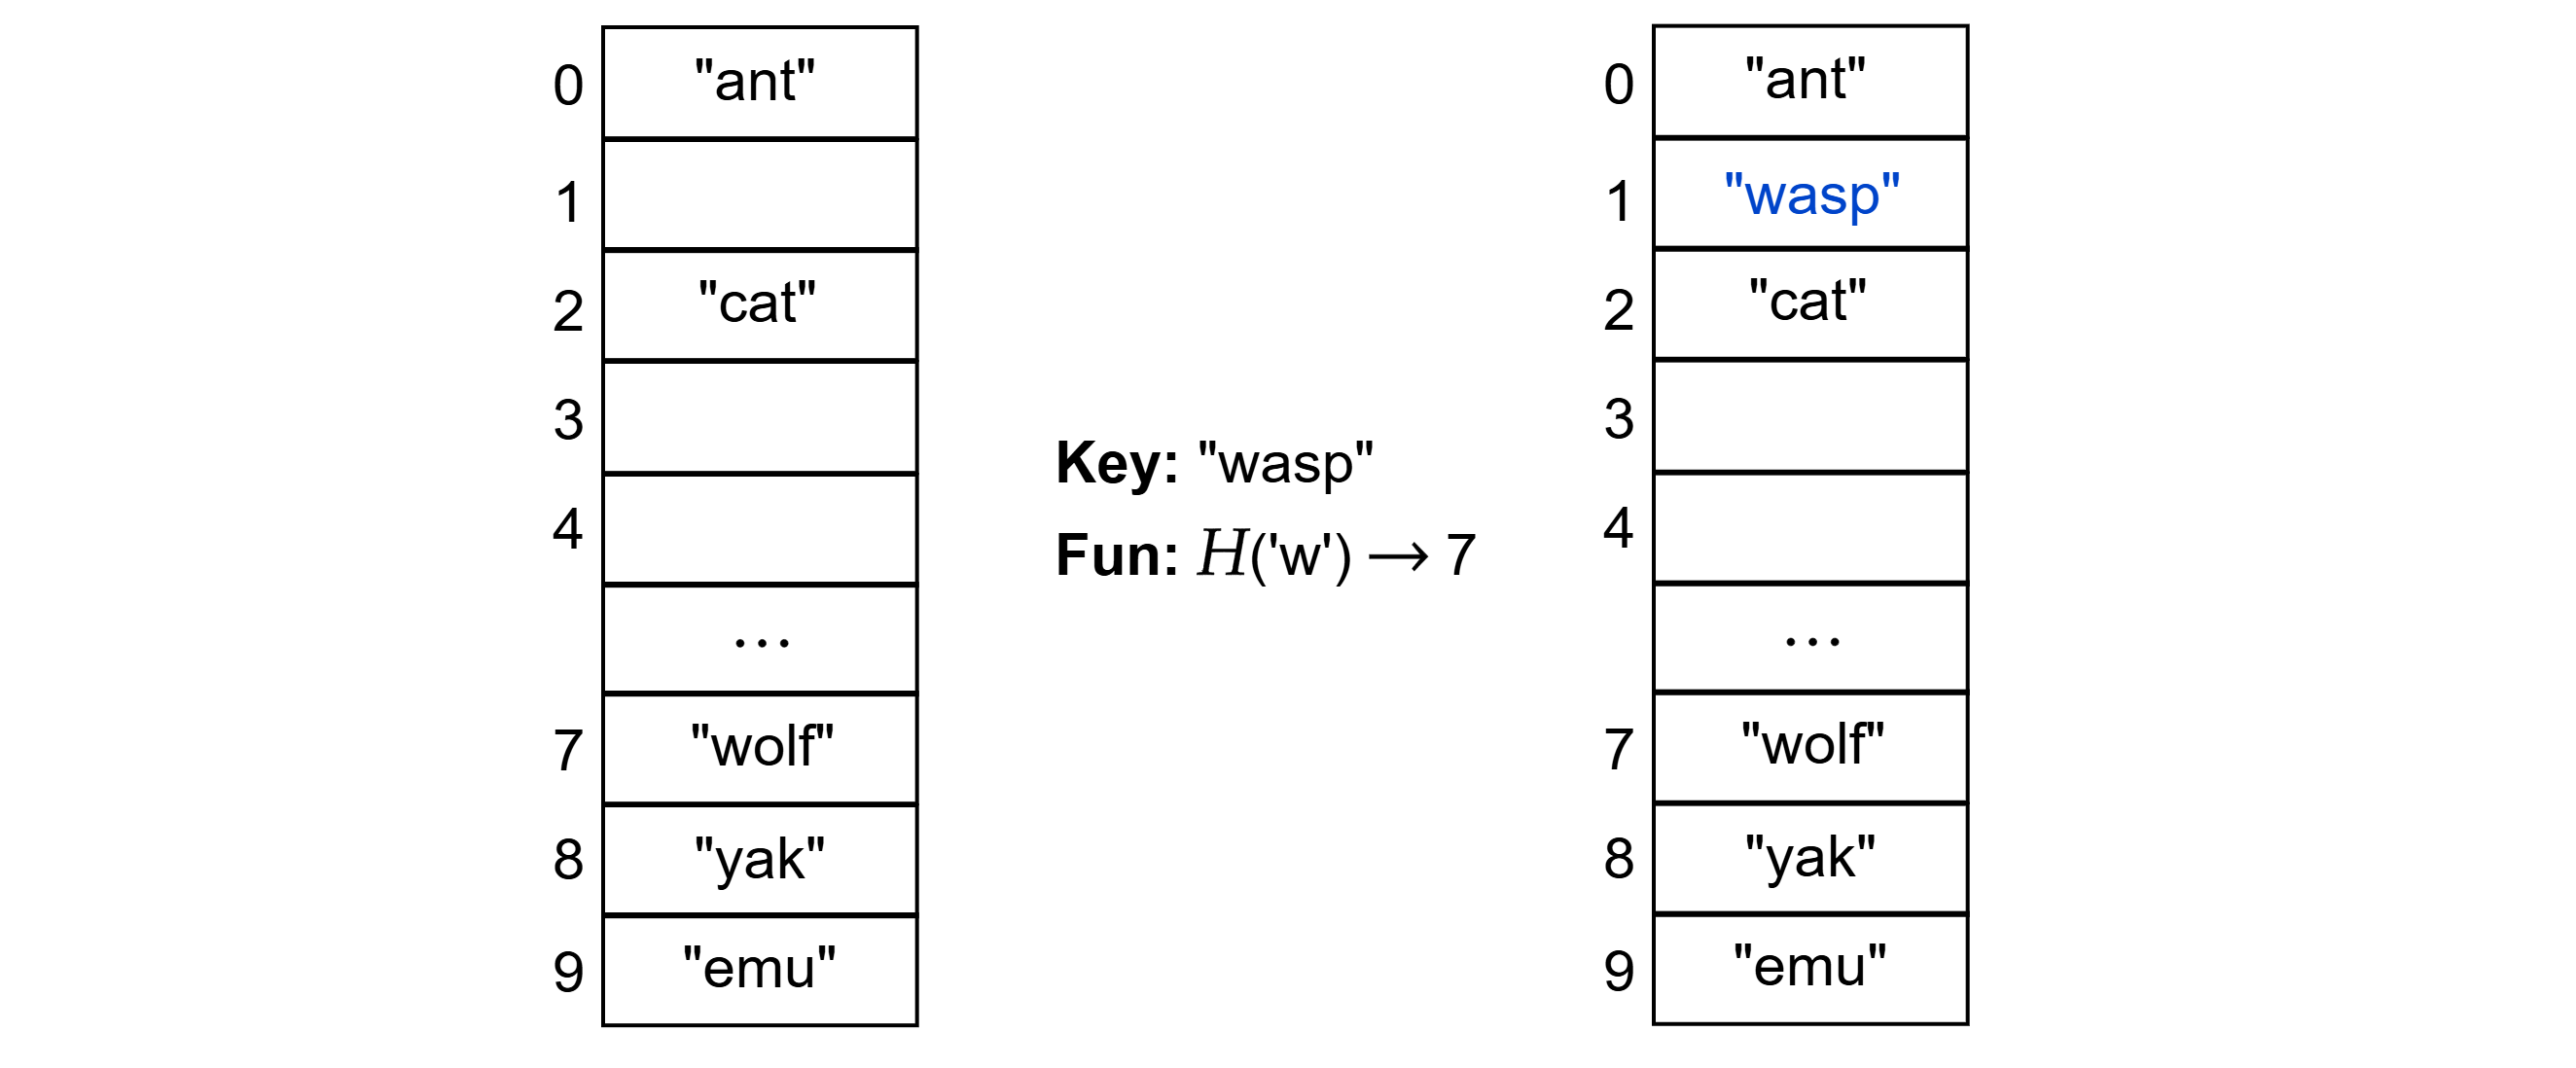
\includegraphics[width=\textwidth]{Sections/hash/open_addressing.png}
    \caption{On the left is an existing hash table of 10 elements filled with various keys. The middle shows the insertion of a new key,
    `wasp', which the function $H$ hashes to index $7$; However, index $7$ already occupied. The algorithm walks through the table, wrapping around
    to the beginning, finding a free index at 1. The right shows the final state of the hash table with `wasp' inserted at index $1$.}
    \label{fig:open_addressing}
\end{figure}

\begin{Def}[Linear Probing]

   \textbf{Linear Probing} in open addressing refers to sequentially checking each index for an available slot (e.g., Figure \ref{fig:open_addressing}).
\end{Def}

\newpage

\begin{Def}[Quadratic Probing]

    Upon finding a collision at index $i$, the next index to check is $(i + k^2)\ \%\ n$, 
    where $k$ is the number of collisions encountered thus far, and $n$ the size of the hash table.
    This is method is called \textbf{quadratic probing}.\\

    \noindent
    \textbf{Note:} It is fully possible to have a free index at $i + 1$, but the algorithm will skip it due to its even probing style.
    We \textbf{terminate execution} once $n$ indices have been checked, avoiding an infinite loop.
\end{Def}

\noindent
So why even use quadratic probing?
\begin{Def}[Clustering]

    \textbf{Clustering} is a phenomenon in open addressing where multiple keys form contiguous \emph{runs} of occupied indices.
    This degrades linear probing performance; Such is the main motivation behind quadratic probing.
\end{Def}

\begin{figure}[ht!]

    \centering
    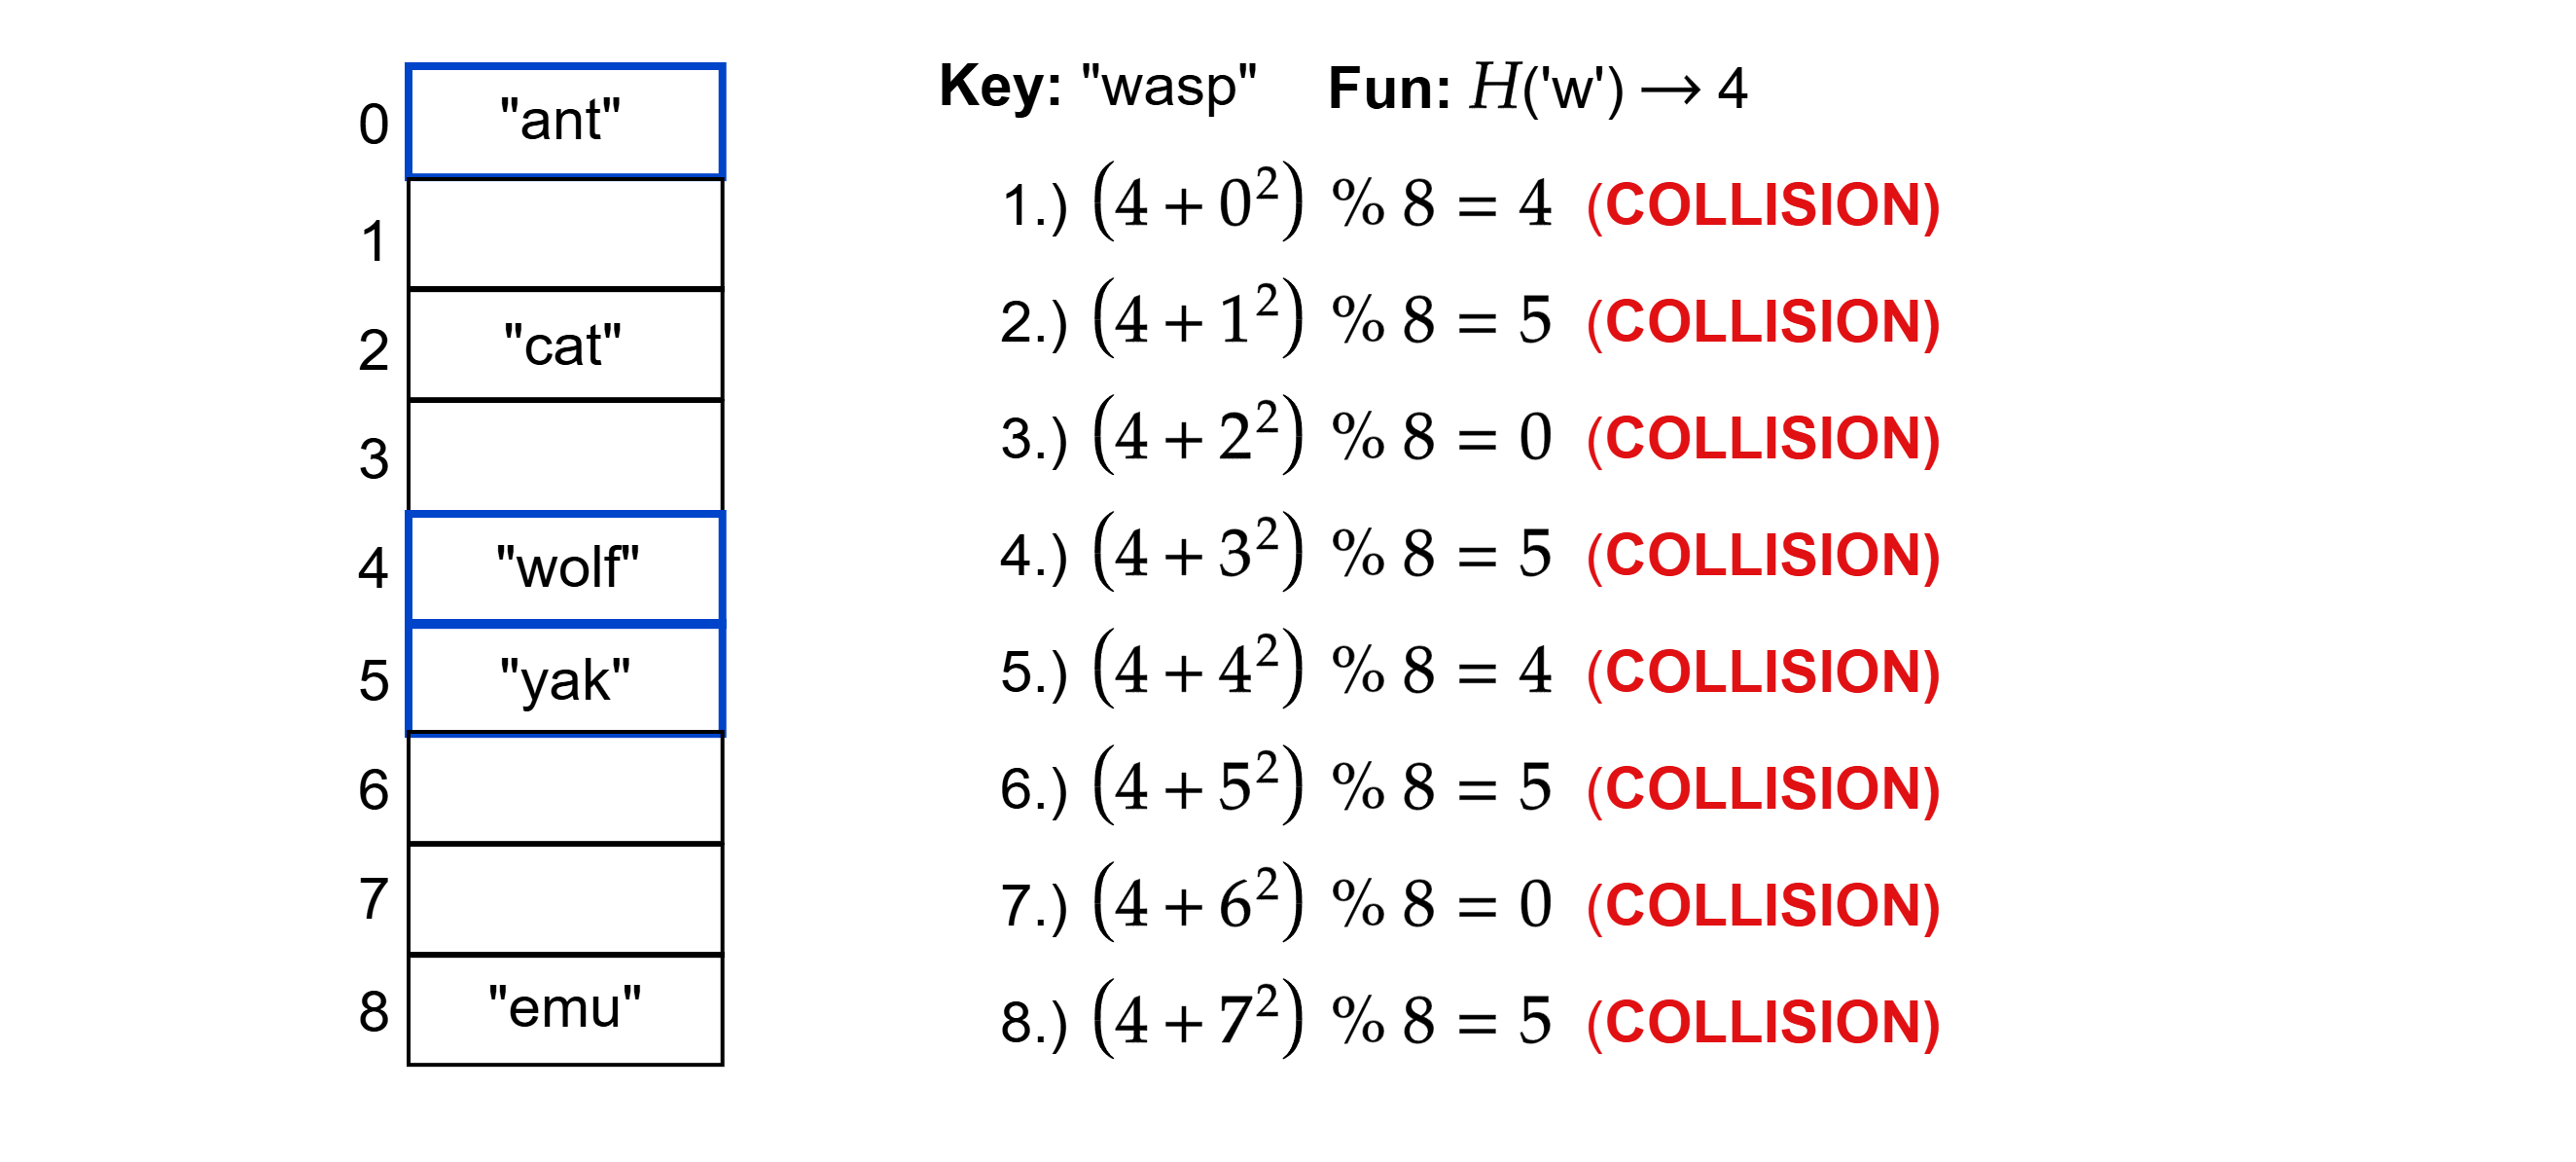
\includegraphics[width=\textwidth]{Sections/hash/quadratic_probing.png}
    \caption{On the left is an existing hash table of 8 elements. We attempt to insert a new key, `wasp', which hashes to index $4$;
    Though, 4 in occupied. The algorithm continues with $(4 + 1^2)\ \%\ 8 = 5$, which is also occupied. After some probing, it appears only indices $4, 5, 0$
    are appearing, from which are all occupied. The algorithm terminates at its $n$-th attempt with $(4+7^2)\ \%\ 8 = 5$. No spaces were found. One could imagine
    that if the table were larger or $0,4,5$ were free, the algorithm would have had better success.}
    \label{fig:quadratic_probing}
\end{figure}


% \newpage
\section{Virtual Memory}

\label{sec:virt}
\subsection{Problem Space of Virtual Memory}
Virtual memory solves three problems \cite{virtualmemory2023}:
\begin{itemize}
    \item \textbf{Not enough memory, Memory fragmentation, and Security}
\end{itemize}
\begin{Def}[Not Enough Memory]

    Back then, computer memory was expensive, and many computers had very little memory (e.g., 4--1 GiB or even less).
    CPUs could only support up to 4 GiB of memory, as CPUs were 32-bit ($2^{32}$ addresses = $2^{32} bytes  = 4 GiB$). 
    On the other hand, 64-bit CPUs can support up to $2^{64}$ addresses = 16 million TB of memory.
\end{Def}

\begin{figure}[h]

    \hspace{-7em}
    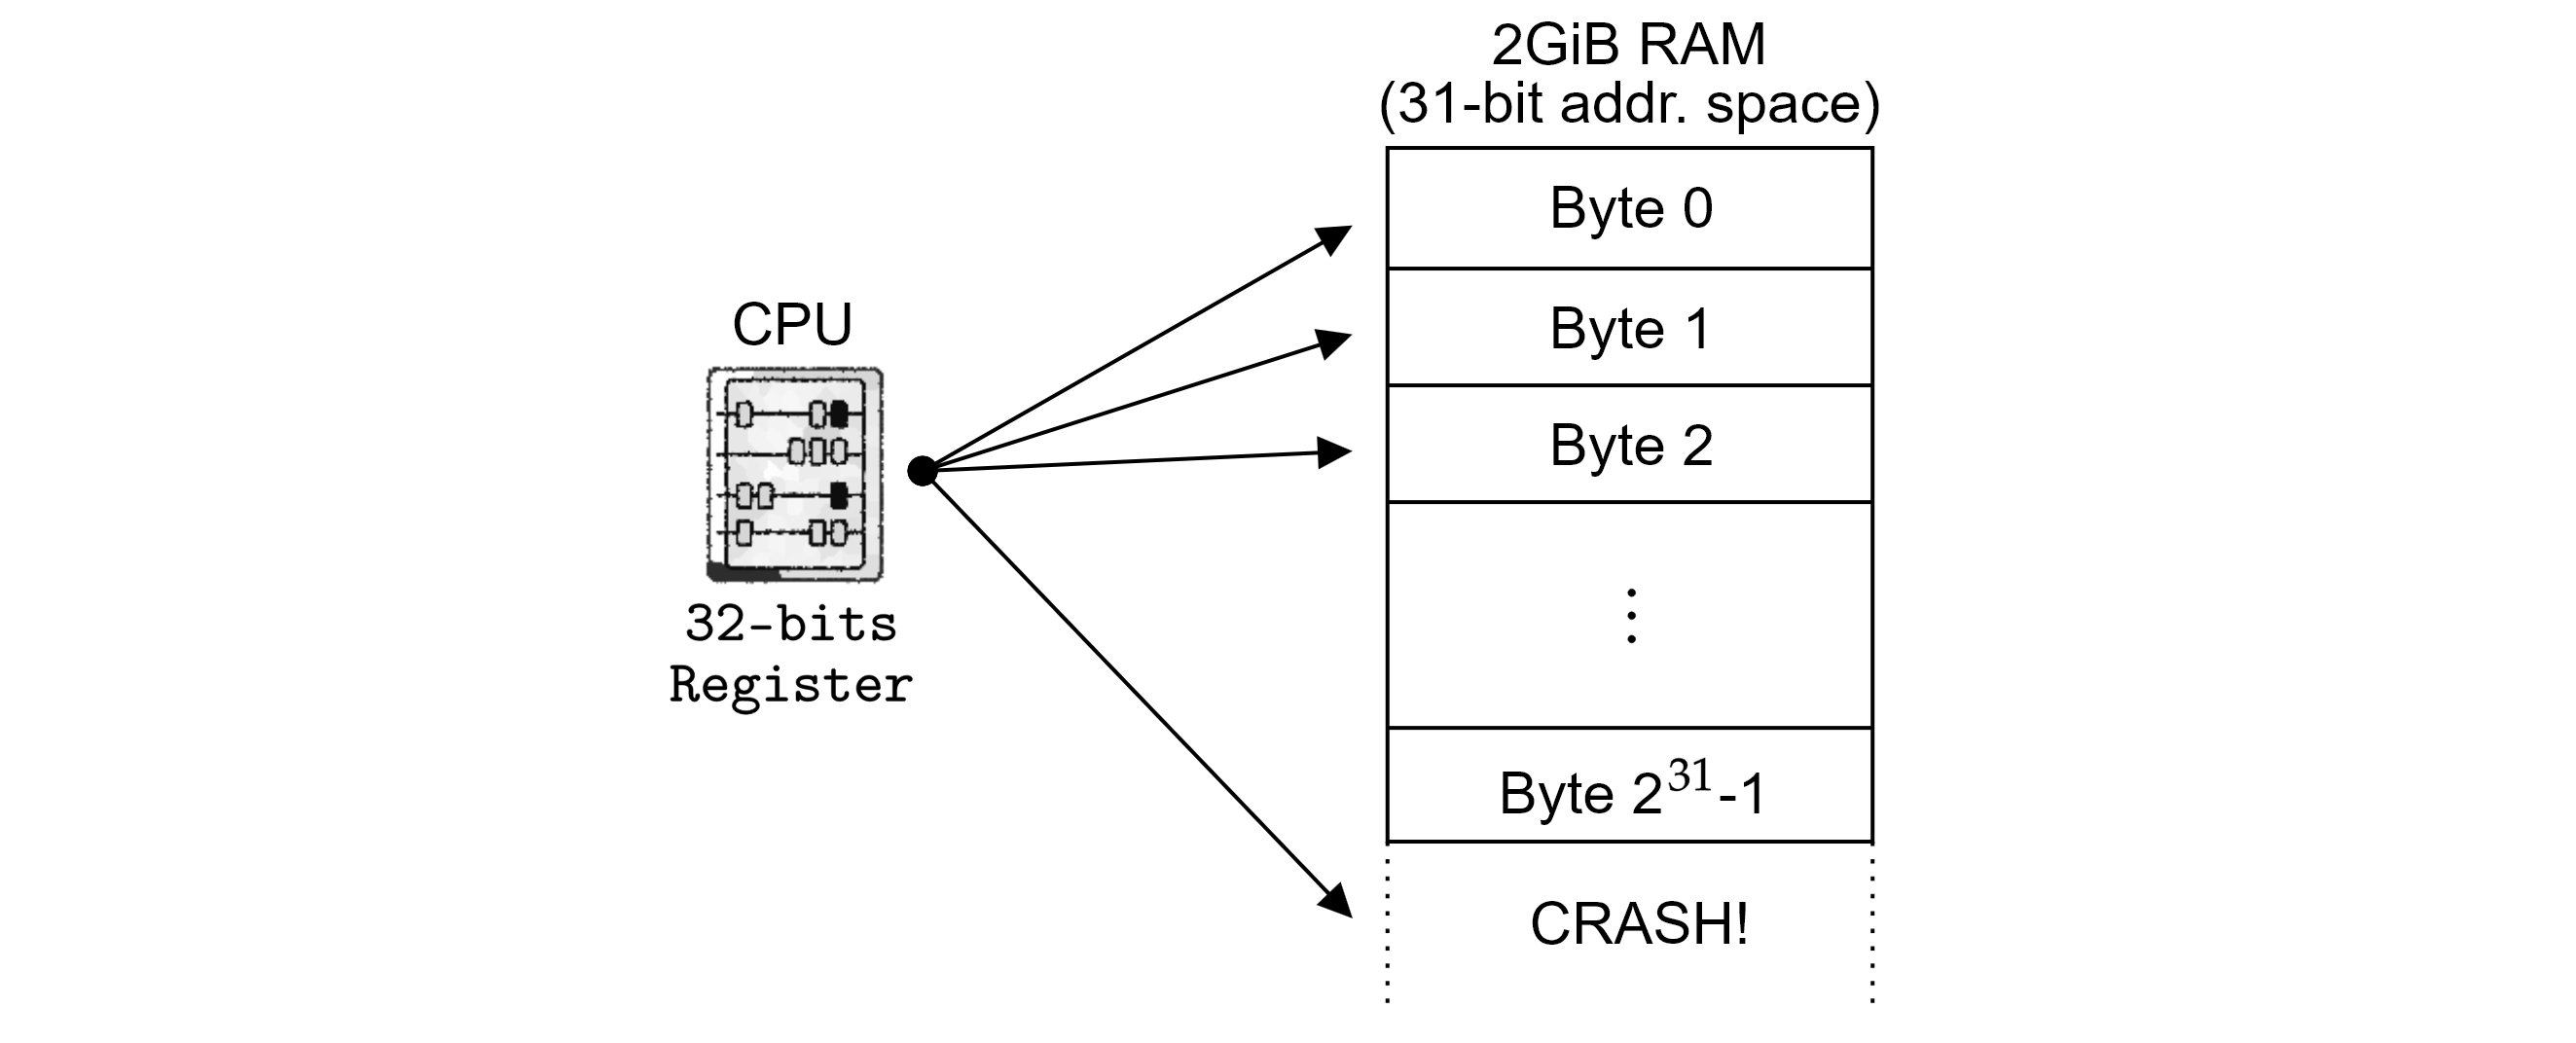
\includegraphics[width=1.3\textwidth]{Sections/virt/crash.png}
    
    \vspace{1em}
    \caption{A 32-bit CPU accessing 2 GiBs of RAM, where a crash happens when trying to access beyond the 31-bit address space.}
    
    \label{fig:virt1}
\end{figure}
\newpage 

\noindent
The next problem deals with multiple processes allocating and deallocating memory:

\begin{Def}[Memory Fragmentation]
    
    Memory can be thought of as a big array, where each cell is a resource a program can use.
    We want memory usage to be contiguous (i.e., no gaps or holes). So say we have an array 
    $$[O, O, O, O]$$

    \noindent
    Where $O$ represents free space in our array, each cell 1 GiB of space. If we have processes $A$ and $B$ take 1 and 2 GiBs respectively, we might have a memory layout of:
    $$[A, B, B, O,]$$

    \noindent
    If we then free process $A$, we might have a memory layout of:
    $$[O, B, B, O]$$
    \noindent
    Now, if another process $C$ needs 2 GiBs of memory, it will not be able to find a contiguous space of 2 GiBs, even though we have 2 GiBs of free space.
    This is called \textbf{memory fragmentation}.
\end{Def}

\noindent
Now finally we have the problem of protecting memory from other processes:

\begin{Def}[Memory Security]

    In a multi-process system, processes may have collisions when trying to access the same memory space.
    For example, if process $A$ is a weather service and process $B$ is some finance service, we don't want 
    the weather service to overwrite the same memory space where the finance service is storing critical data.
    This is called \textbf{memory security}.
\end{Def}

\noindent
So in theory we want to give each process it s own portion of memory, to solve overlapping access:
\begin{Def}[Virtual Memory]

    To solve process memory collisions, we give each process its own fictional view of memory, called \textbf{virtual memory}.
    Though for this to work, each virtual view is mapped to an actual place in the original memory we call \textbf{physical memory}.\\

    \noindent
    \textbf{Virtual and physical addresses} are the cells spaces themselves.
\end{Def}

\newpage 

\noindent
Consider the figure below showing how virtual memory works in theory:

\begin{figure}[h]
    \centering
    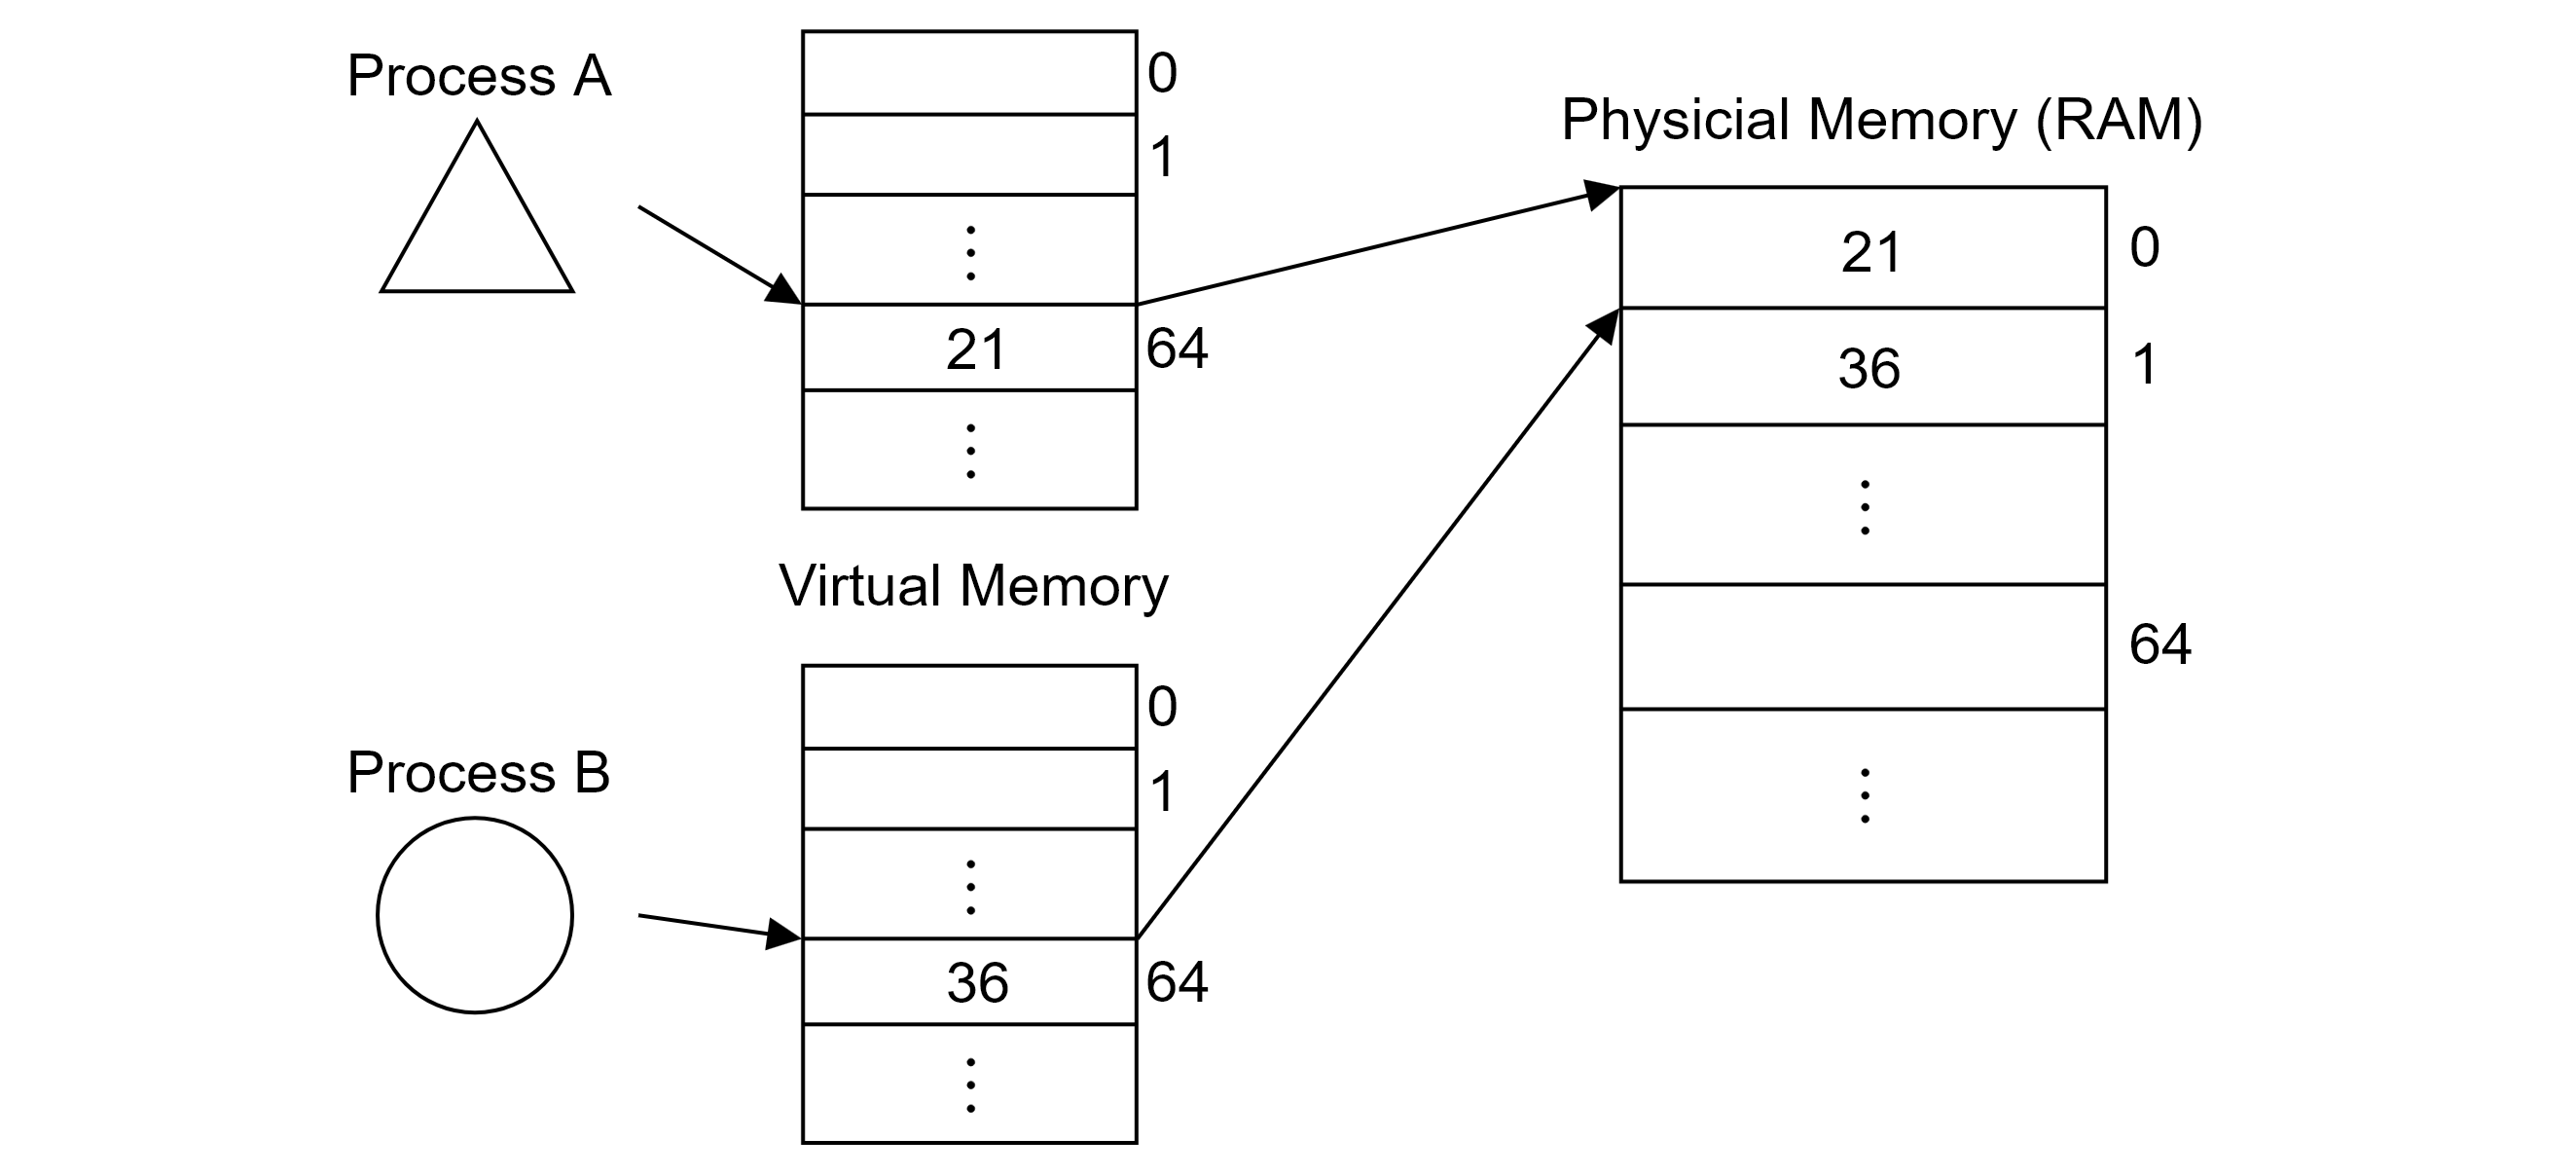
\includegraphics[width=\textwidth]{Sections/virt/virt.png}
    
    \vspace{1em}
    \caption{Processes $A$ and $B$ write to memory cell $64$ in their view of memory, but in reality they map 
    to different physical memory cells (0 and 1 respectively).}
    
    \label{fig:virt2}
\end{figure}

\noindent
A quick aside:

\begin{theo}[Physical Memory the CPU Accesses]

    In reality the CPU can access the physical memory of many other devices (e.g., hard drives, SSDs, etc.). In 
    addition, the OS takes up some of the physical memory as well. The rest is left to programs to use. The 
    program allocated space is the memory we refer to going forward as the \textbf{physical memory}.
\end{theo}

\noindent
Virtual memory solves the three problems we mentioned before:
\begin{Def}[Virtual Memory \& Not Enough Memory (Swapping)]

    The physical memory can be much smaller than what a program thinks it has in virtual memory. When a program tries to access memory 
    it does not have, the OS will \textbf{swap} physical memory to external storage to free up space. This means, while a program is not using 
    a portion of memory at a given time, the OS can swap it in and out depending on system needs.\\

    \noindent
    Memory that is swapped out is called \textbf{swap-memory}. Every time a we try to access such absent memory 
    in our mappings, it's called a \textbf{page fault} (more on this later).
\end{Def}

\newpage
\begin{Def}[Virtual Memory \& Fragmentation]

    Virtual memory allows programs to think they have contiguous memory. This simplifies their 
    memory management, while in reality the OS manages the split memory mappings.
\end{Def}

\begin{figure}[h]
    \centering
    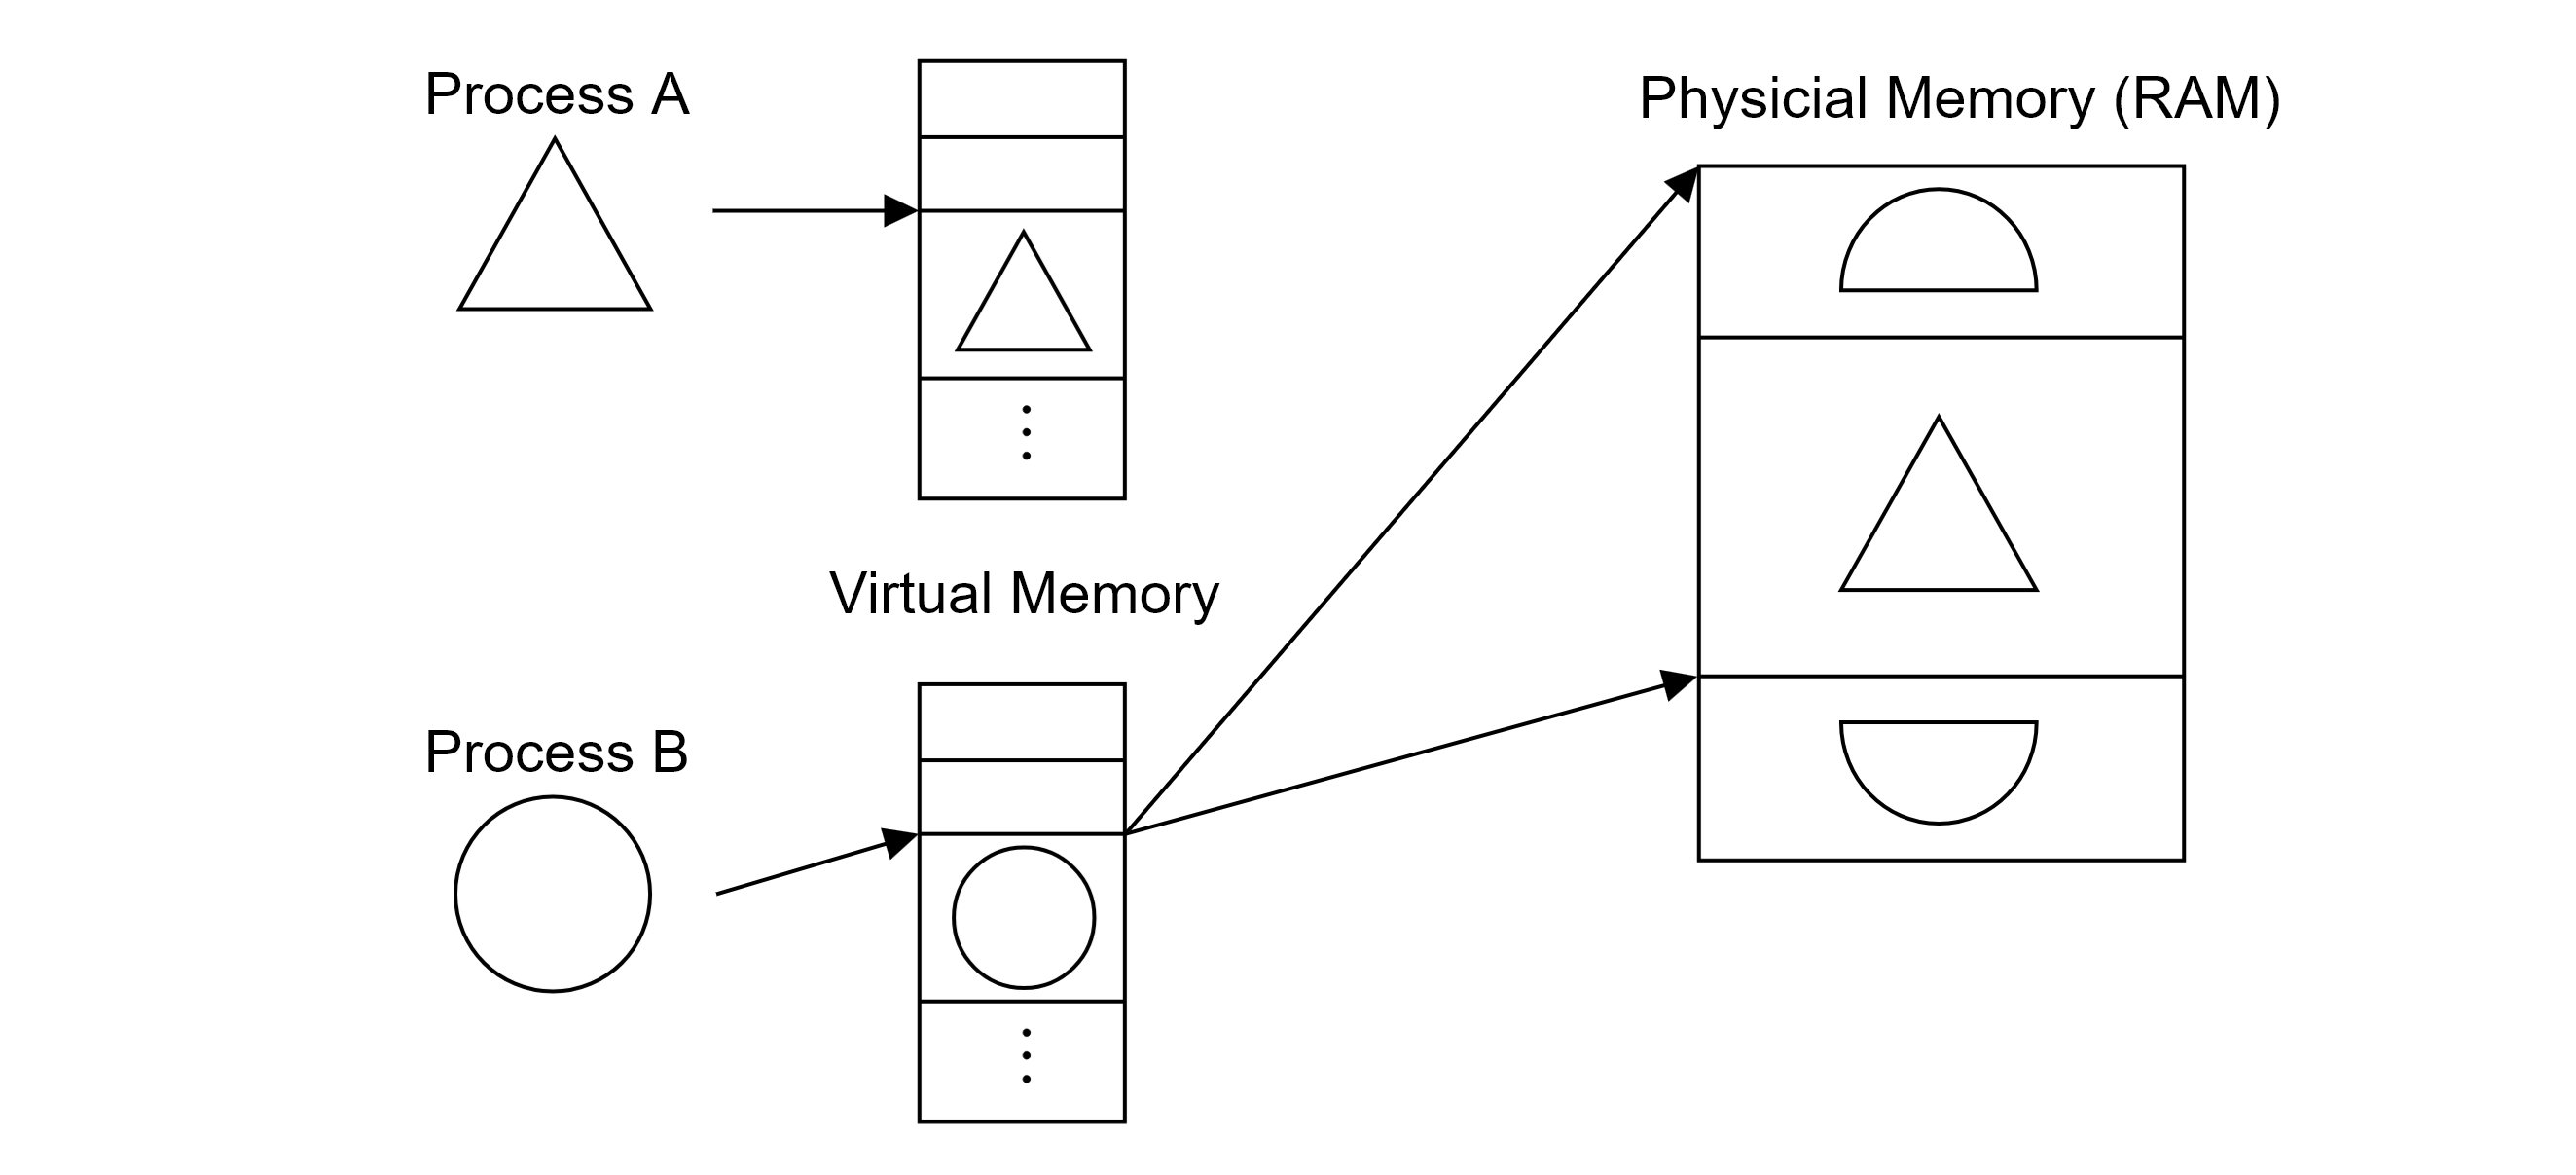
\includegraphics[width=\textwidth]{Sections/virt/frag.png}
    
    \vspace{1em}
    \caption{Here two processes $A$ and $B$ are using the same physical memory space. Both think they have 
    contiguous memory, but in reality, $B$ is split into two parts in the physical memory.}
    
    \label{fig:virt3}
\end{figure}

\begin{Def}[Virtual Memory \& Security]

    Memory cells are collision safe as memory mappings are not shared in physical memory; However, this would be 
    inefficient if say $A$ and $B$ depend on a secondary process $C$. In this case, $A$ and $B$ may share the same mapping to $C$'s memory.
\end{Def}

\subsection{Virtual Memory Implementation (Page Tables)}
\noindent
We discuss the mapping mechanism further in linking virtual to physical memory.
\begin{Def}[Page Tables]

    The OS keeps a \textbf{page table}, where each entry is a mapping of a virtual memory cell to a physical one, called a \textbf{Page Table Entry (PTE)}.
    CPUs work with words (32 bits = 4 bytes), so the page table has one entry for every word (address) in the virtual memory space.
\end{Def}

\newpage 

\noindent
We make the following observation:
\begin{theo}[Theoretical Page Table Space Complexity]

    If our CPU 32-bits, then there are $2^{32}$ addresses. CPUs speak in words, hence we'd need $2^{30}$ words, and thus $\approx$ 1 billion PTEs (4 GiB per table).
    This is too much memory to practically implement for each process.
\end{theo}

\noindent
We solve the above problem, via the following strategy:

\begin{Def}[Memory Chunking (Pages)]
    
    Instead of mapping each address to a PTE---which would be too large. We
    chunk the memory into \textbf{pages} reducing the number of PTEs needed. Typically, page sizes 
    are some power of 2, most commonly 4 KiB (4096 bytes), meaning 1024 words per page. This reduces our 
    page table requirement from 4 GiB to 4 MiB (1 Million PTEs). Despite moving 4 KiBs of data at a time, this works
    well in practice, as adjacent memory is often accessed together. 
\end{Def}

\begin{figure}[h]
    \centering
    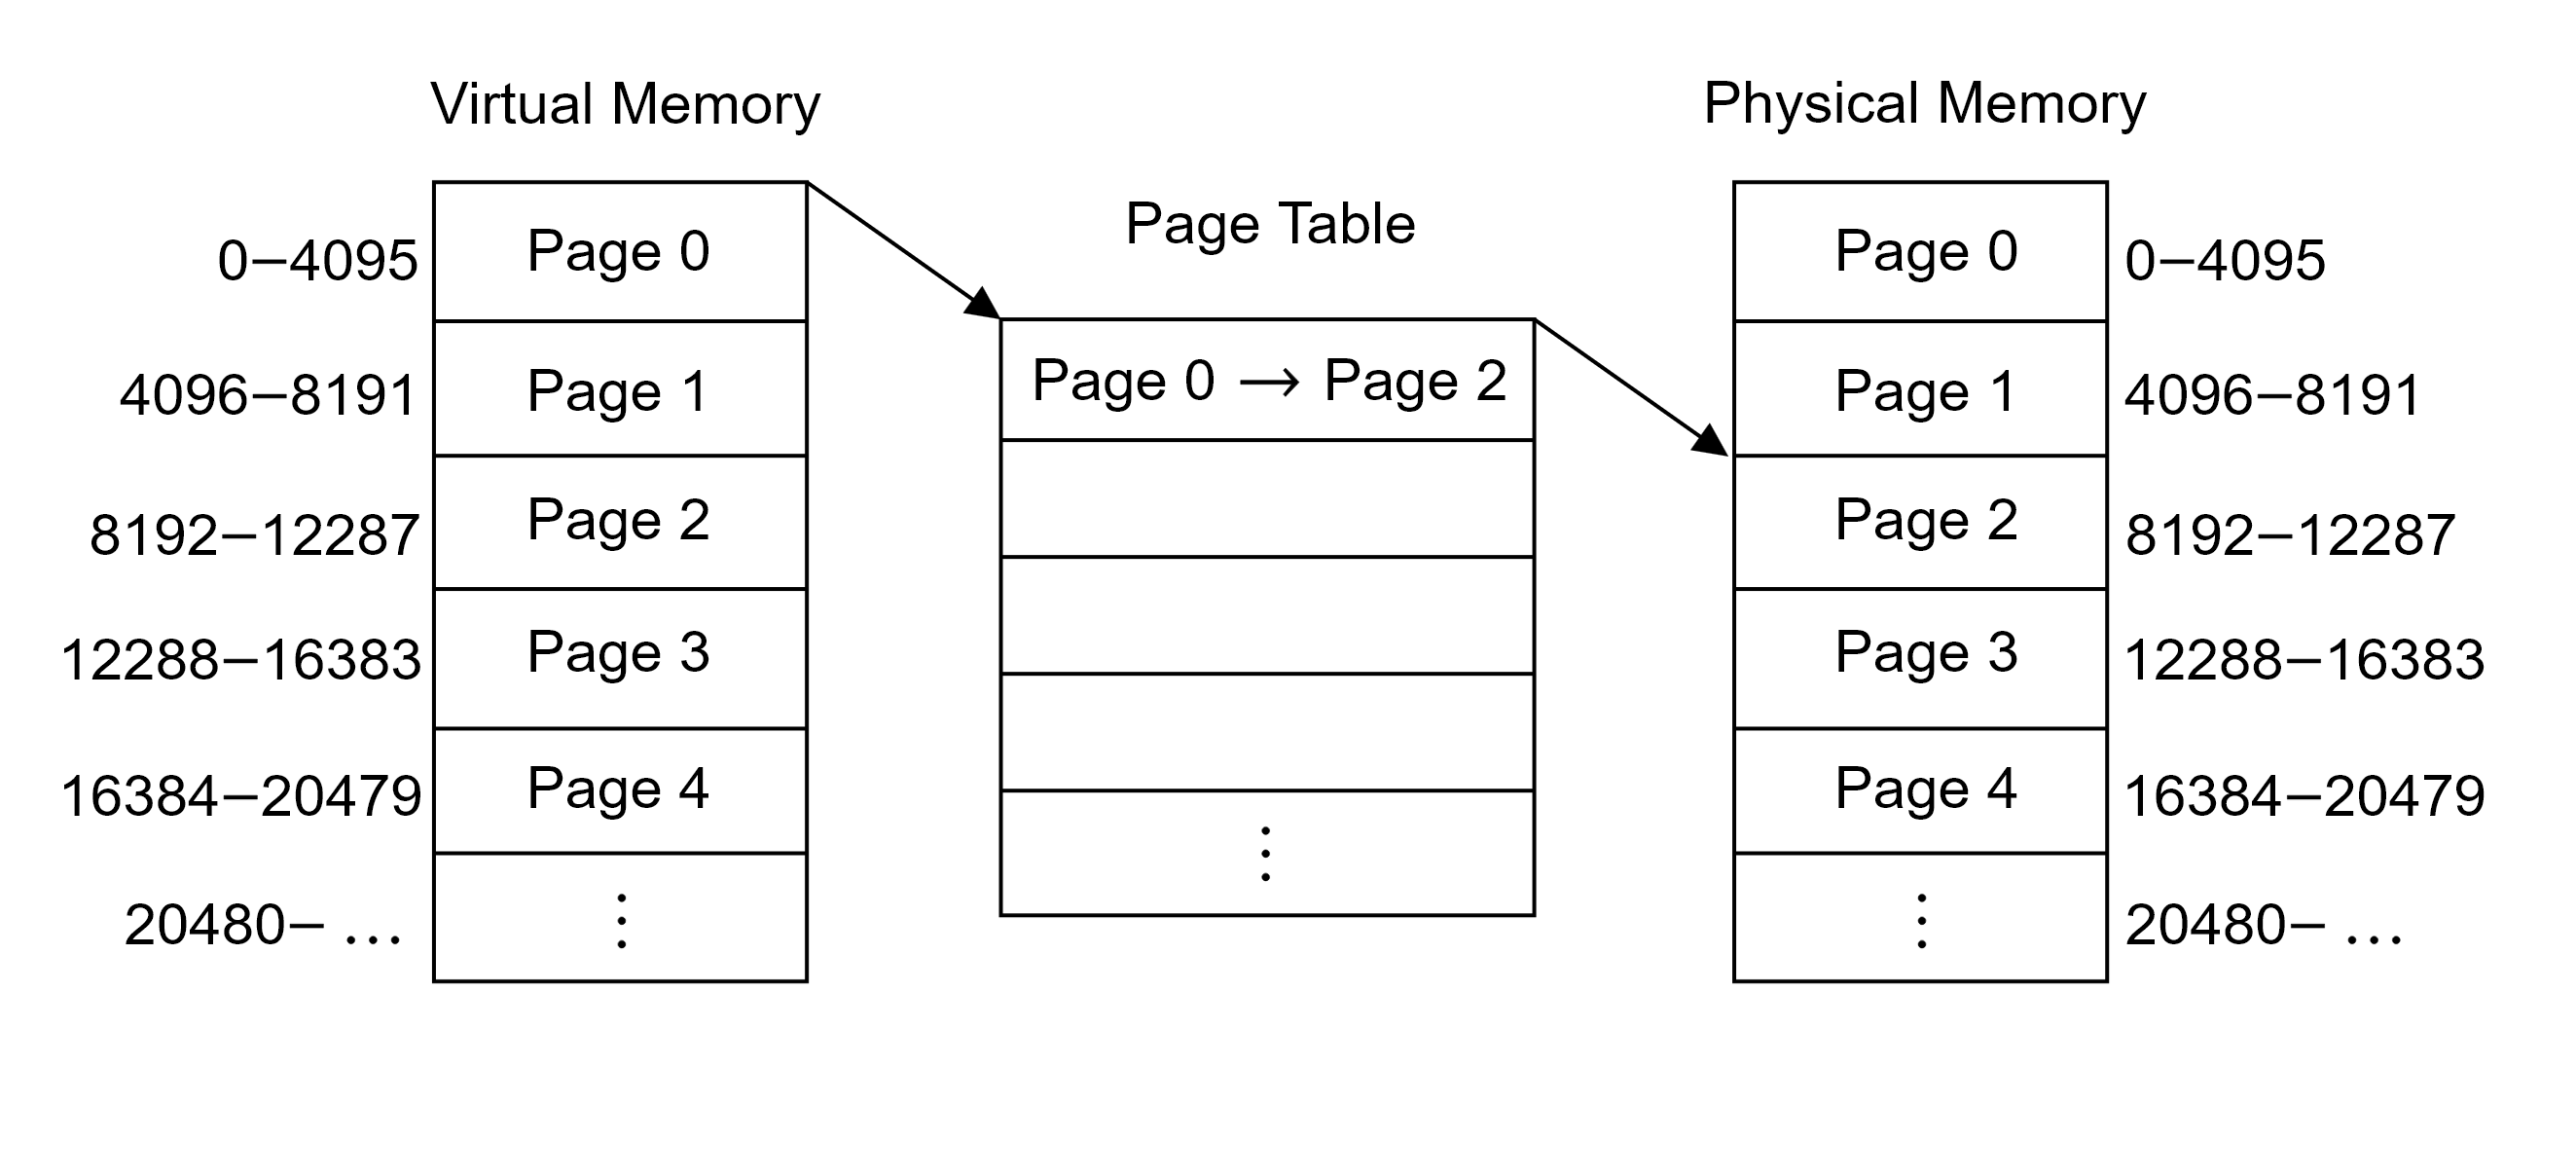
\includegraphics[width=\textwidth]{Sections/virt/page.png}
    
    \vspace{1em}
    \caption{A 4 MiB page table, each PTE 4 KiB (4096 bytes, 1024 words), showing mappings.}
    
    \label{fig:virt4}
\end{figure}


\noindent
One must ask themselves:
\begin{itemize}
    \item What is the relationship of how the Page Numbers are separated.
    \item Can we determine the page number given a specific address?
    \item How might we convert a virtual to a physical address given some address?
\end{itemize}
\noindent
We discuss the following on the next page.

\newpage 
\begin{Example}[Converting Virtual to Physical Memory (intuition)]

    \label{theo:virt2phys}
    We may find conversions from virtual to physical memory via the following formula: $$\text{PA} = \underbracket{(\text{VA}\ \%\ \text{Page Size})}_{\text{offset}} + \underbracket{(\text{Page Size} \cdot \text{Physical Page Number})}_{\text{Physical Page starting index}}$$
    \noindent
    Where $\%$ is modulo and Page Number = $\left\lfloor \frac{\text{Addr.}}{\text{Page Size}} \right\rfloor$. \textbf{However,} this is not the most efficient way,
    and is \underline{strictly for educational/intuition building} purposes.\\

    \noindent
    \rule{\textwidth}{0.4pt}\\

    \noindent
    Given the Figure (\ref{fig:virt4}), $104\to 8296$ from $104 + 4096 * 2 = 8296$.
\end{Example}
\begin{theo}[Converting Virtual to Physical Memory]

    Addresses are binary numbers, typically represents as hexadecimal (base 16) numbers.


    The first 12 bits of an address is the \textbf{offset}. The remaining higher-order bits yields the \textbf{page number}. To find the physical address, take the last 12 bits of the address, index the higher-order bits into the page table, and append the offset to the physical page number.
\end{theo}

\begin{figure}[h]
    \centering
    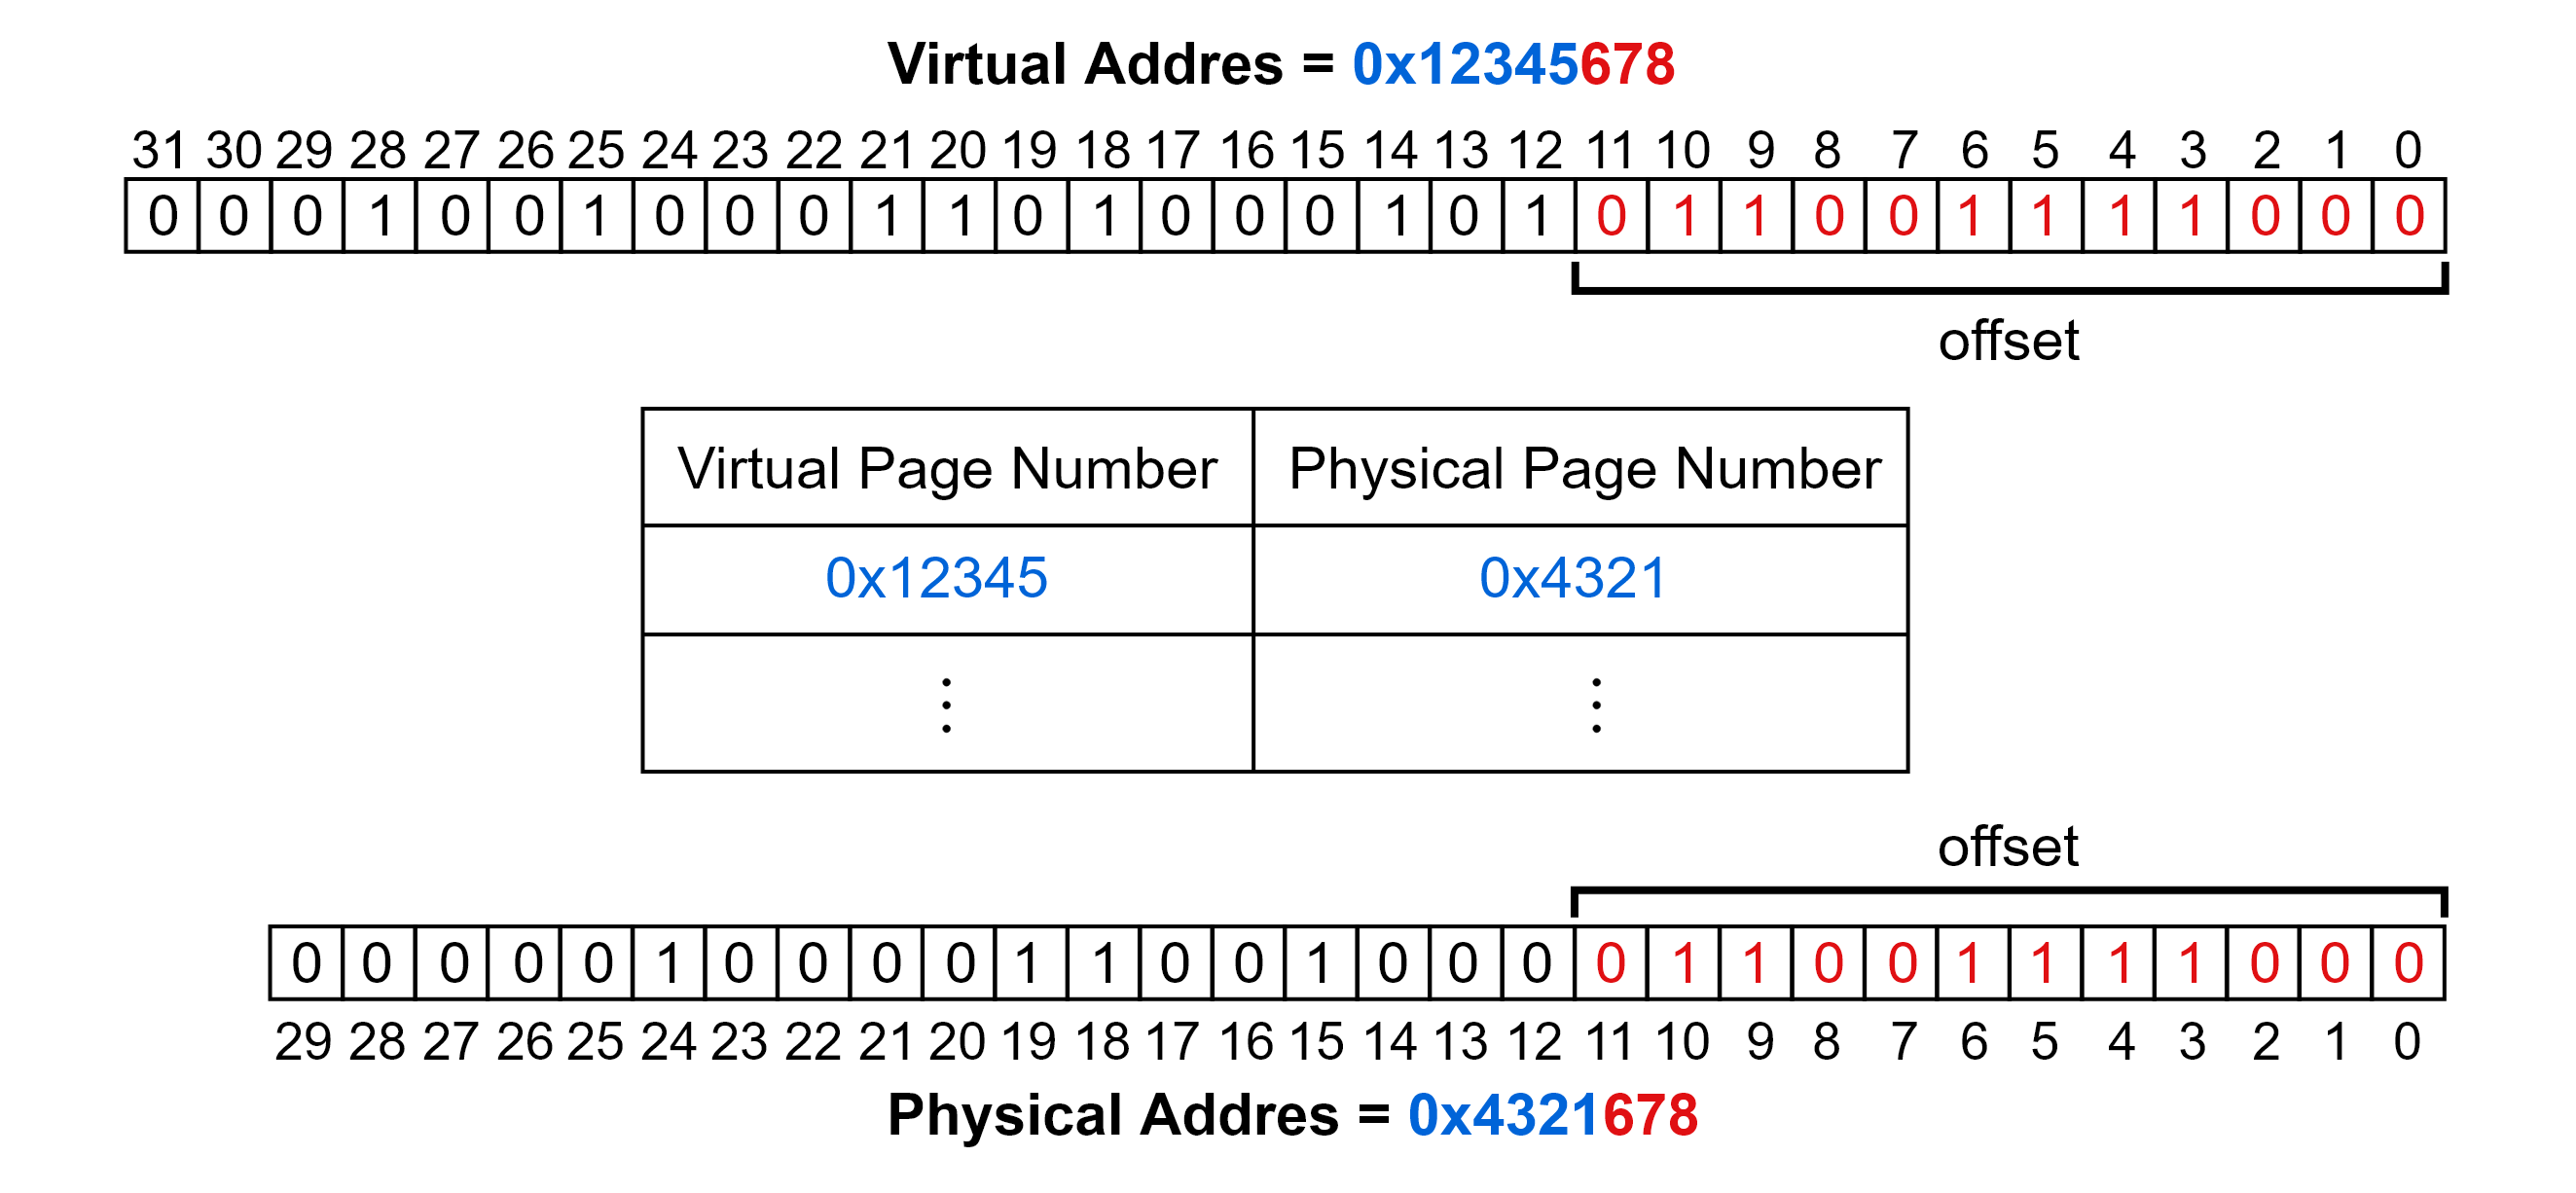
\includegraphics[width=\textwidth]{Sections/virt/conv.png}
    
    \vspace{1em}
    \caption{The conversion of 0x123456 (32-bit, 4 GiB) $\to$ 0x4321678 (30-bit, 1 GiB). Recall that if a accessing a page that is not in memory, causes a page fault, from which the OS with begin to swap memory with external storage devices.}
    
    \label{fig:virt5}
\end{figure}

\newpage 

\subsection{Page Faults \& Translation Lookaside Buffer (TLB)}

So far we have discussed how the mapping system of virtual memory works, but now we pivot to how the OS handles swapping data in and out of memory on page faults.

\begin{Def}[Swapping on Page Faults]

    A \textbf{page fault} occurs when a program tries to access a page that does not have a mapping in the page table. 
    The OS then picks the \textbf{least recently used (LRU)} page in the page table, and swaps it out to external storage. A page is \textbf{dirty} if it has been written to. In 
    such case, we write back its contents to external storage before swapping. If the page is not dirty, we may discard it on swap.
\end{Def}

\vspace{-1em}
\begin{figure}[h]
    \centering
    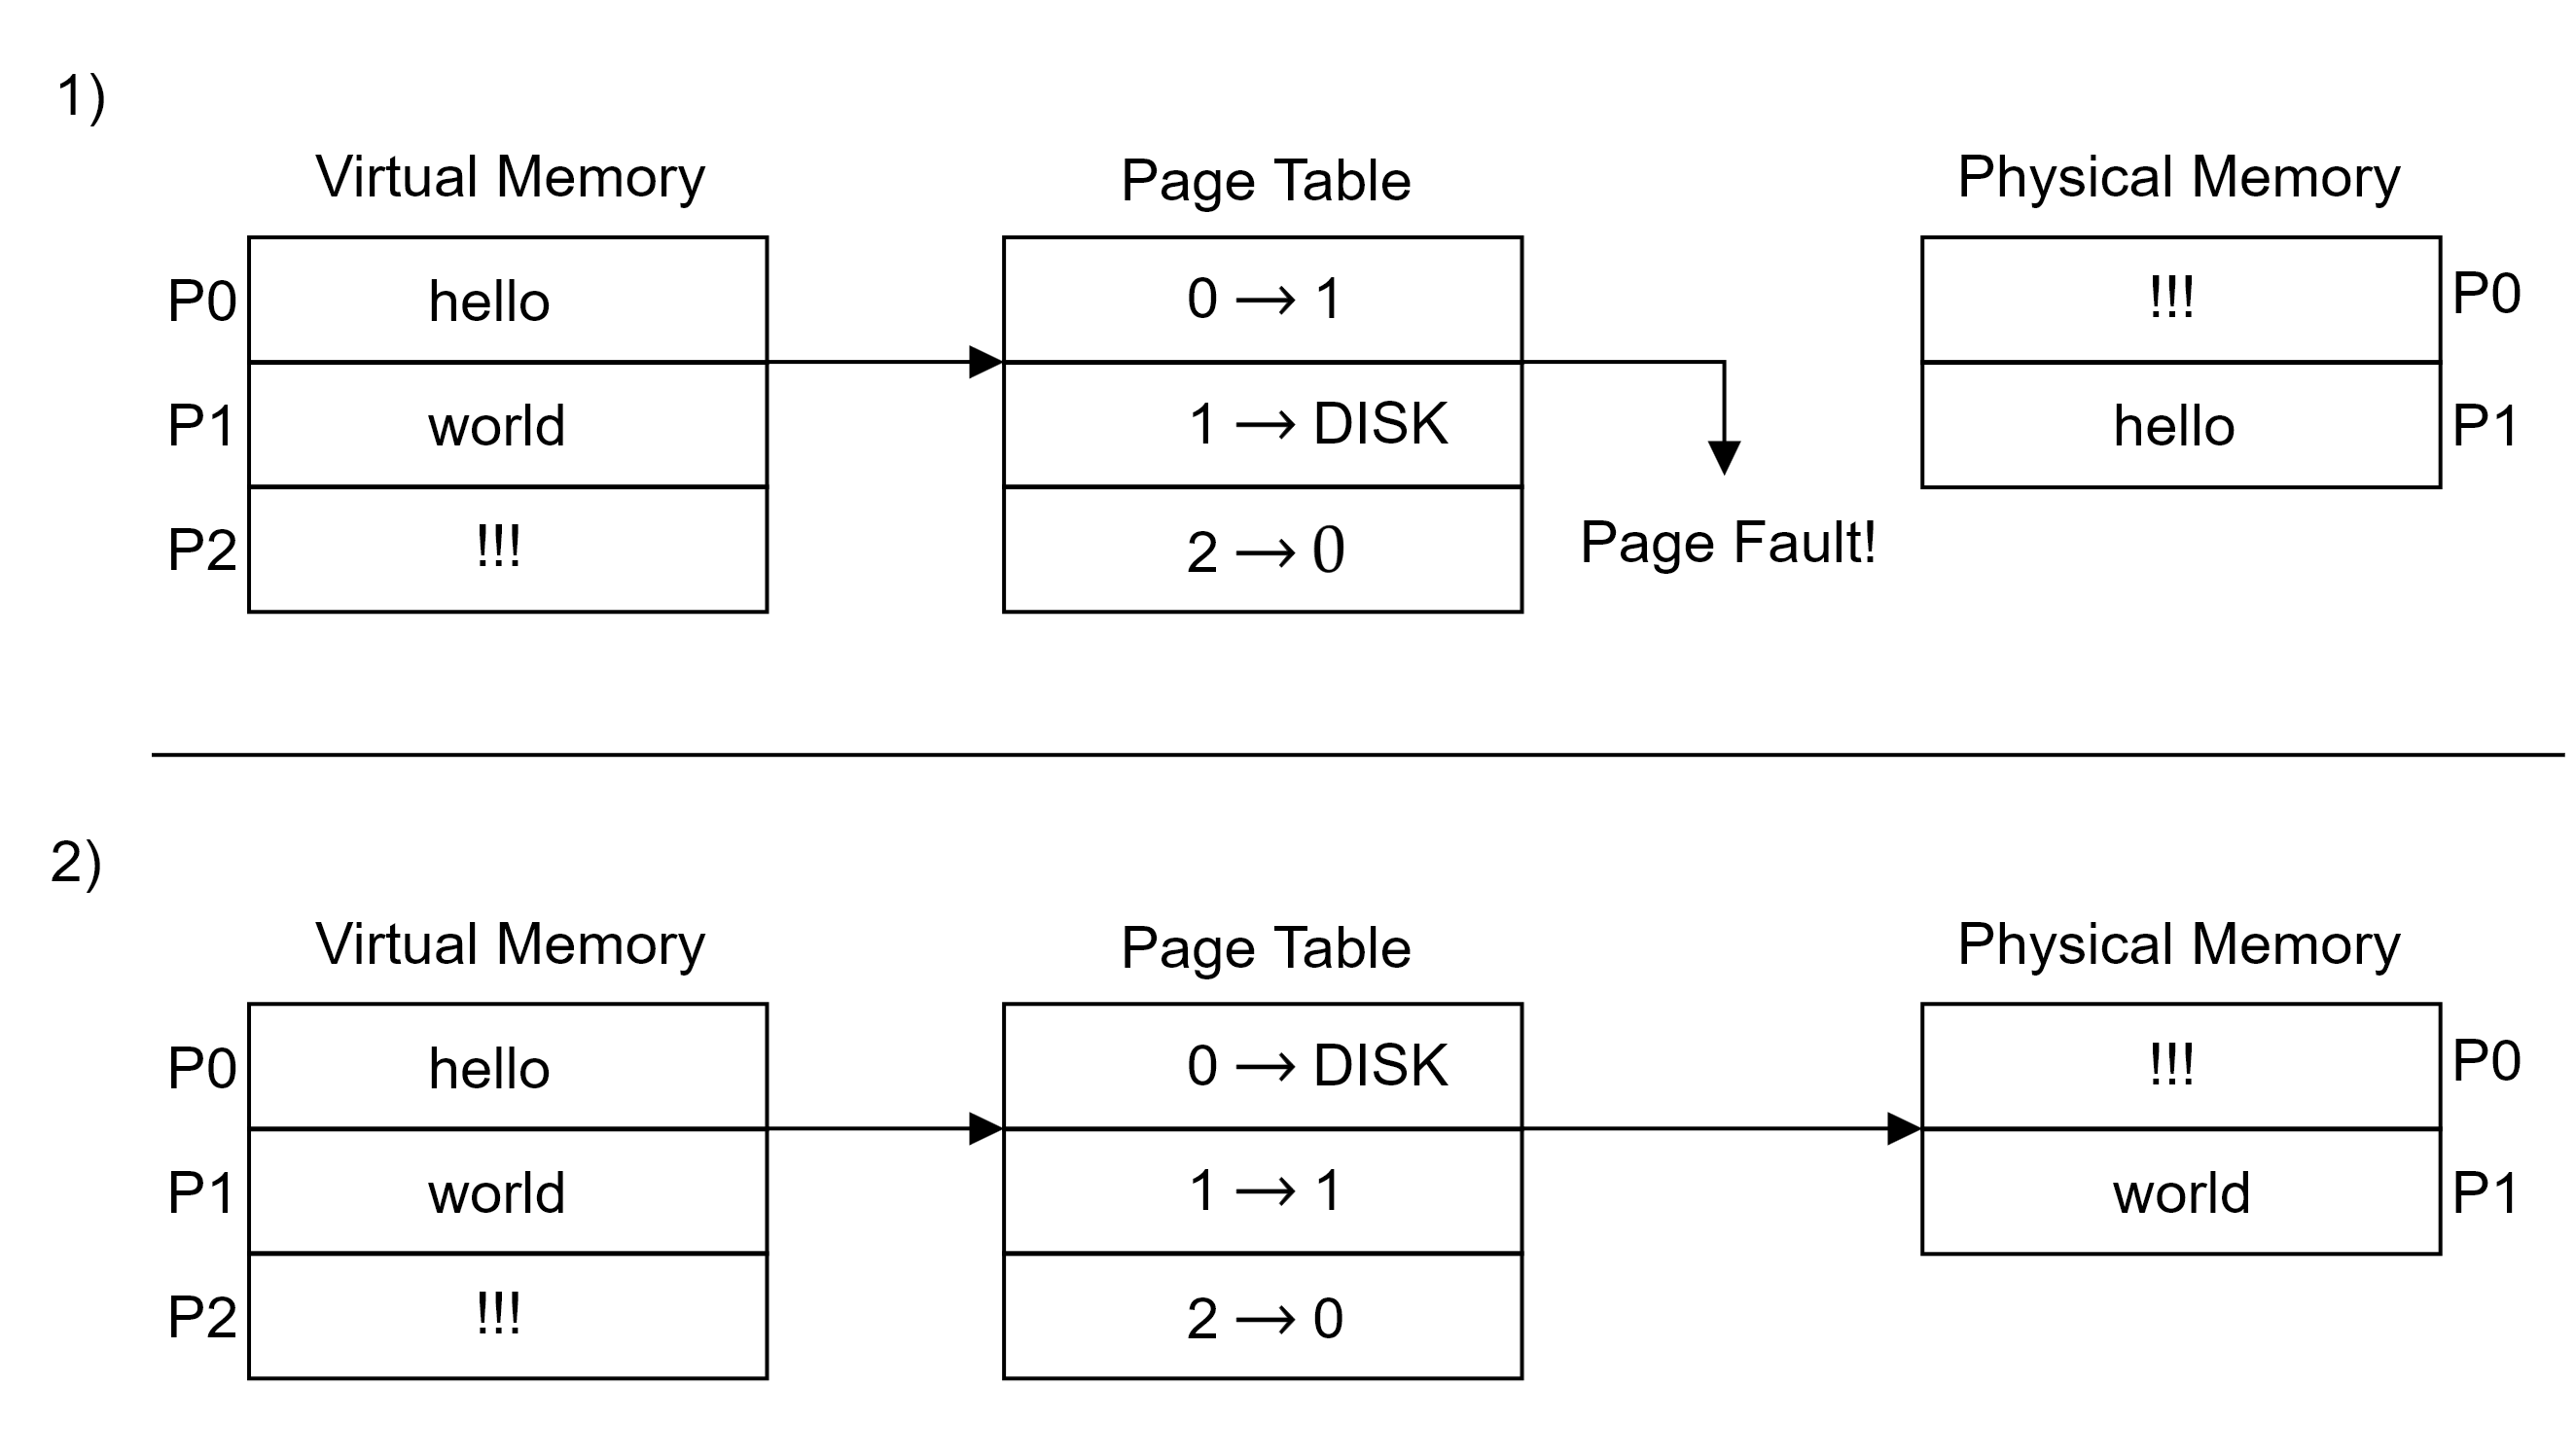
\includegraphics[width=\textwidth]{Sections/virt/pagefault.png}
    
    \vspace{1em}
    \caption{
        1) A page fault occurs when trying to access page 1. 2) The OS has swapped out page 0 to external storage (DISK), and now page 1 can be accessed.
        Note: This diagram is for illustrative purposes, virtual memory does not contain data, only addresses binding to physical memory.
        }

    \label{fig:virt6}
\end{figure}

\begin{Def}[Direct Memory Access (DMA)]

    Page faults are expensive, as swapping data with I/O devices may take some time. Modern CPUs have a \textbf{Direct Memory Access (DMA)} module, which allows I/O devices to access memory directly, while the CPU completes other tasks. 
\end{Def}

\noindent
Still our routine of mapping is expensive in it of itself.
\begin{Def}[Translation Lookaside Buffer (TLB)]

    The mapping process includes three steps:
    \begin{enumerate}
        \item Index the page table: Access Memory (RAM).
        \item Convert Addresses: Computation.
        \item Interact: Access Memory (RAM).
    \end{enumerate}
    \noindent
    To speed this up, we create a small cache of the most recent Page Table Lookups, called the \textbf{Translation Lookaside Buffer (TLB)}. If a 
    page in not in the TLB, we must preform the translation then load it into the TLB for future use.\\

    \noindent
    Every successful TLB lookup is called a \textbf{hit}, while a failed lookup is called a \textbf{miss}. The \textbf{hit time} and \textbf{miss time} are the time it takes to access the TLB and page table respectively (measured in CPU clock cycles).
    The \textbf{hit rate} is the ratio of hits to the total number of lookups.\\

    \noindent
    Modern CPU architectures usually have two TLBs, one for instructions (\textbf{ITLB}) and one for data (\textbf{DTLB}).
\end{Def}

\begin{figure}[h]
    \centering
    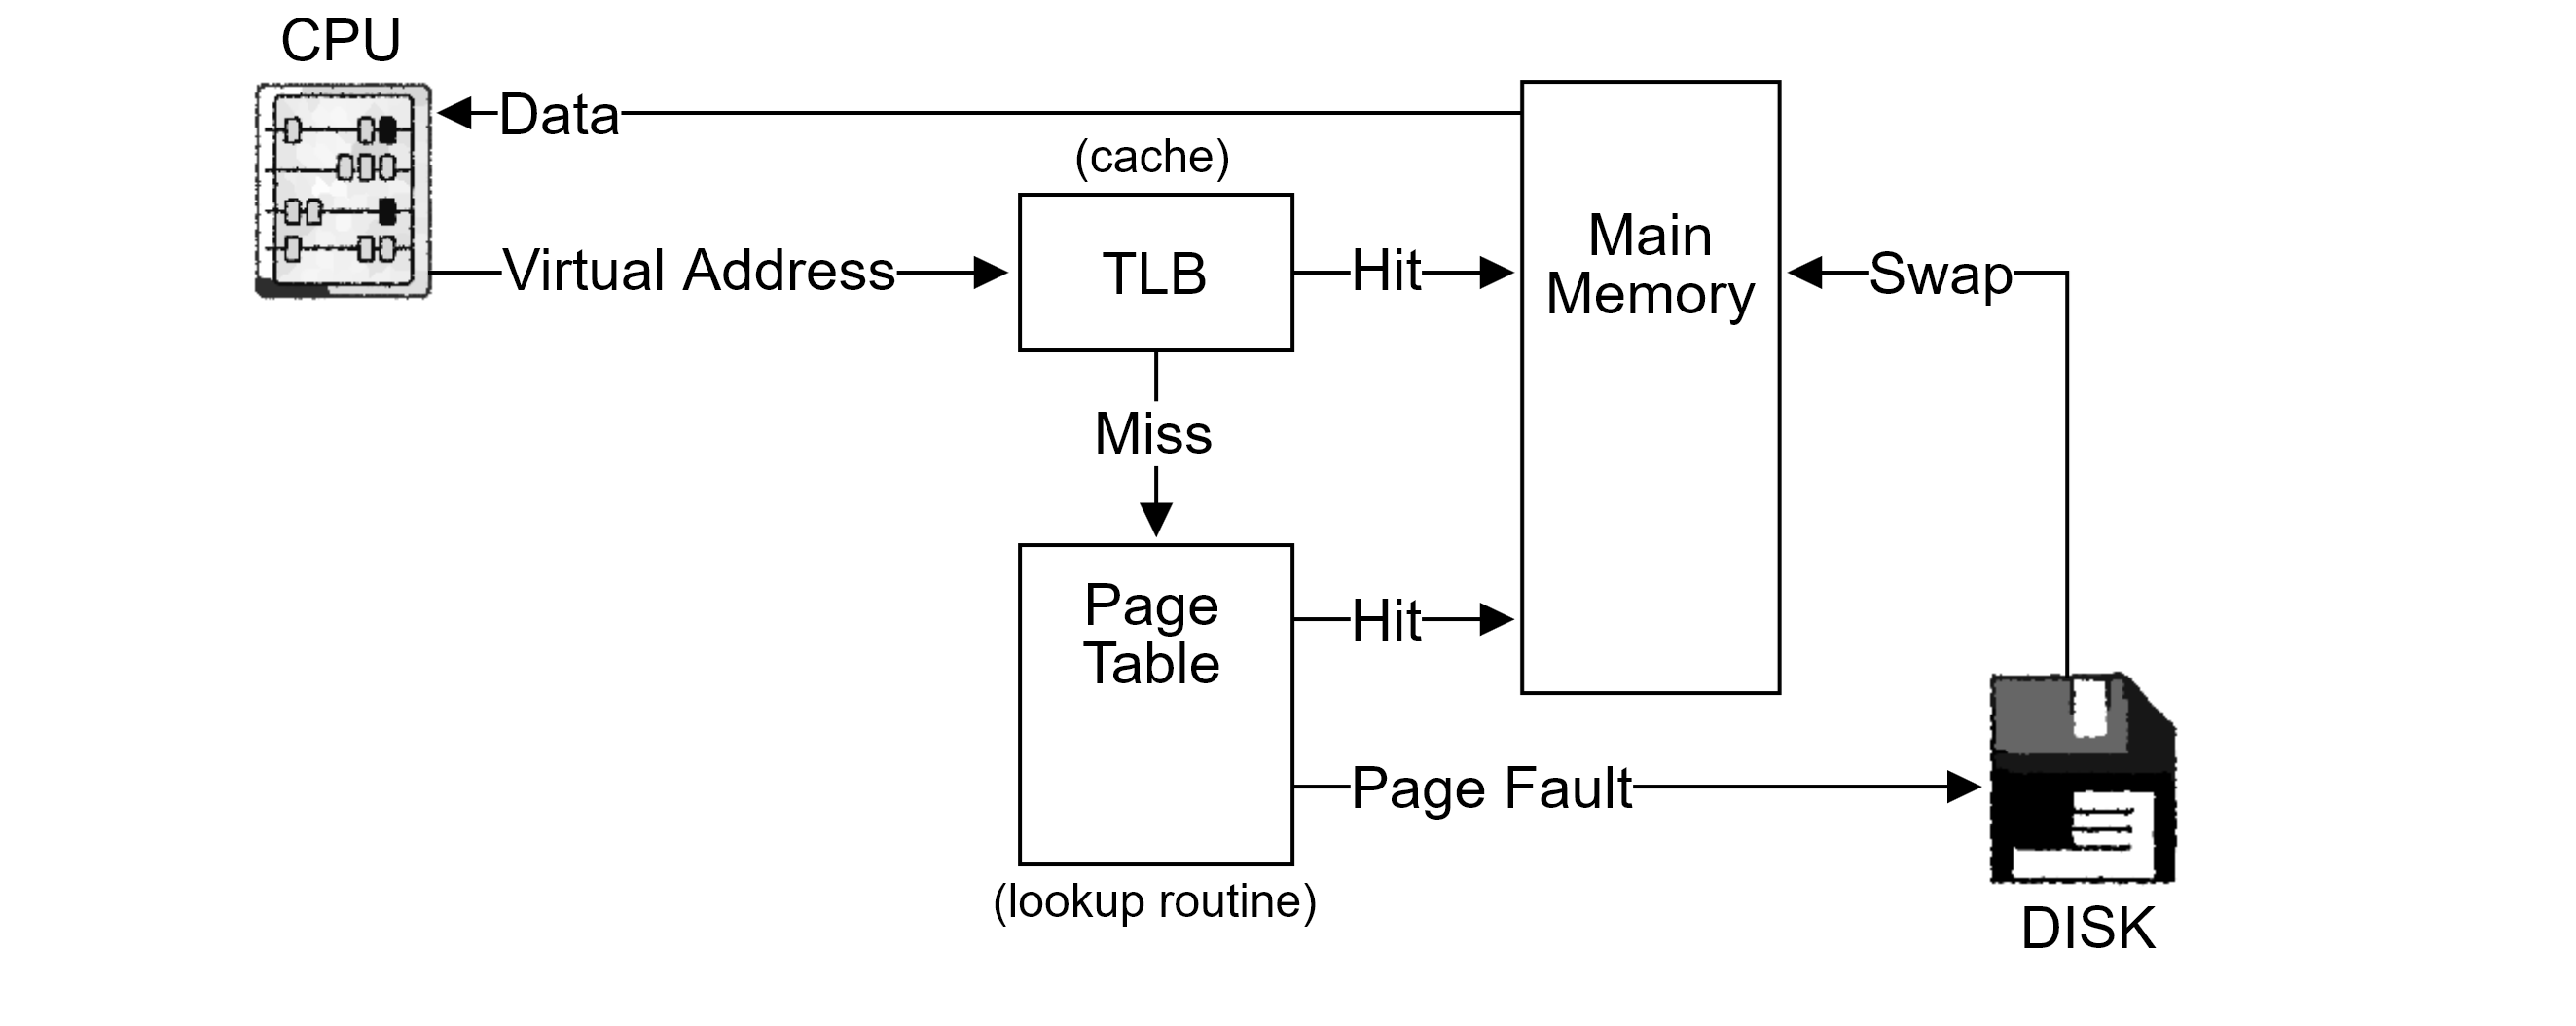
\includegraphics[width=\textwidth]{Sections/virt/tlb.png}
    
    \vspace{1em}
    \caption{Demonstrating how a TLB lookup effects the memory access flow. CPU attempts to access memory providing 
    the virtual address to the TLB. (Happy path) A hit occurs, memory is accessed and passed to the CPU. (Ok path) A TLB miss occurs, causing a page table lookup. A page table hit occurs, the mapping is cached and the memory is accessed. (Sad path) both a TLB and page table miss occurs, causing a page fault. The OS must decide 
    which page to swap out. After swapping, the addressed is cached and the memory is accessed.}
    
    \label{fig:virt7}
\end{figure}

\newpage 
\noindent
So far what we've been covering actually resides within the CPU architecture:
\begin{Def}[Memory Management Unit (MMU)]

    The \textbf{Memory Management Unit (MMU)} is a hardware component that manages the mapping of virtual to physical memory. It is responsible for translating virtual addresses to physical addresses, and it also handles page faults and TLB lookups.
\end{Def}

\subsection{Multi-level Page Tables}

\noindent
Let's define the problem space of multi-level page tables \cite{neso_vm_multilevel}:
\begin{theo}[Single Level Page Table Cost]

    In a 32-bit system, each page table requires 4 MiB of memory. If we had 100 programs running, that's easily 400 MiB of memory.\\

    \noindent
    Additionally, if we move page tables to disk (external storage), we lose any reference we had to them in an attempt to free up memory. So we need to keep some reference oracle in memory.
\end{theo}

\noindent
This highlights the need for a more efficient way 
\begin{Def}[Multi-level Page Tables]

    Recall that in a 32-bit system, we have 4 GiB of memory. In single level page tables, we chunk our addresses into 4 KiBs (4096 bytes), 
    and load all of them at once. That's
    $$4 \text{ KiB} \cdot 1024 \text{ PTEs } = 4096 \text{ KiB} = 4 \text{ MiB }$$

    \noindent
    We wish to offload data without losing references. To do this we allocate a single chunk of memory (4 KiB) to 
    serve as an reference oracle, called the \textbf{page directory} or \textbf{1$^{st}$ level page table}. Each entry in the page directory points to other chunks from which we are safe to load and unload out of memory.
    These referenced chunks are called the \textbf{2$^{nd}$ level page tables}. Each entry in the 2$^{nd}$ level page table points to a physical page.
\end{Def}

\begin{Def}[Converting Virtual to Physical Memory (Multi-level)]

    In multi-level page tables, the first 12 bits are the \textbf{offset}, the next 10 bits are the index into the \textbf{second-level page table}, and the last 10 bits are the index into the \textbf{first-level page directory}. These tables are treated as arrays: indexing the first table yields the address of the second table, and indexing the second table yields the physical page number.
\end{Def}

\newpage 

\noindent
Recall, in single-level page tables the higher 20 bits are the page number and the index, which yields the physical page number.
Multi-level breaks away from this, and instead as illustrated below:
\begin{figure}[h]
    \centering
    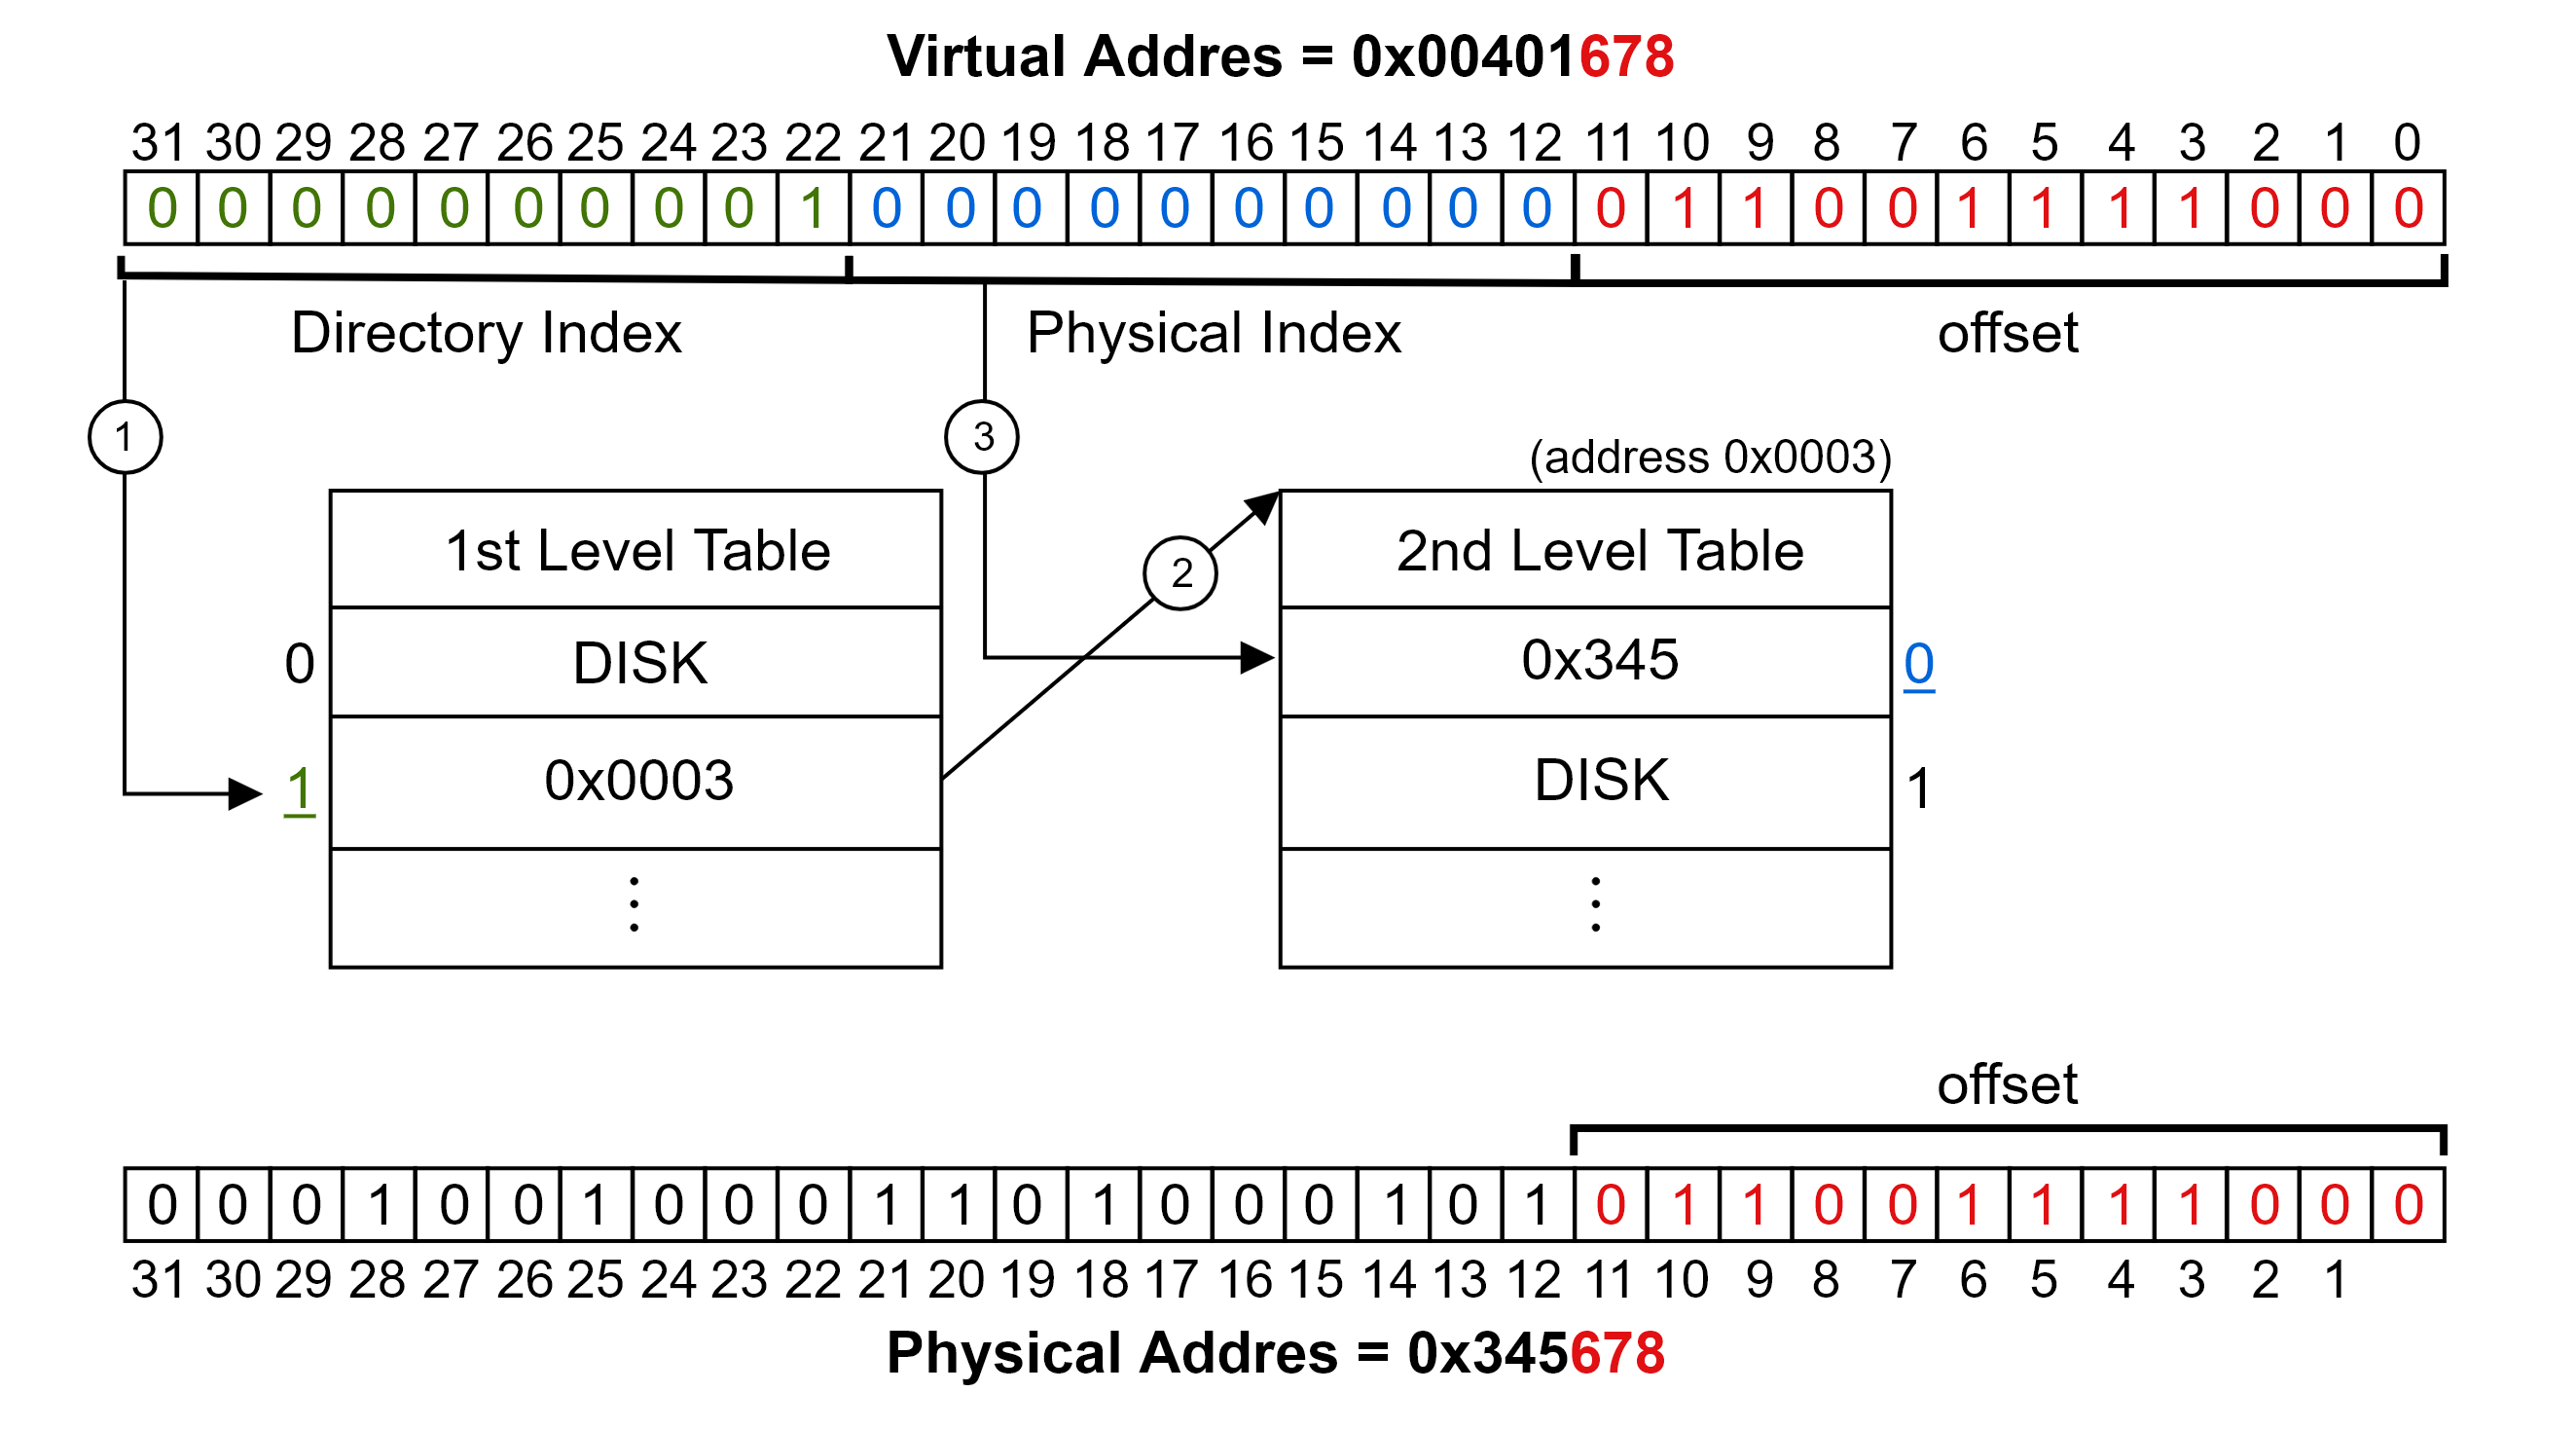
\includegraphics[width=\textwidth]{Sections/virt/level.png}
    
    \vspace{1em}
    \caption{A multi-level page table, where the first level is a page directory, and the second level is a page table which points to physical pages.}
    
    \label{fig:virt8}
\end{figure}

\begin{Def}[Multi-level Page Scaling (64-bit)]

    Increasing the number of bits allows us to scale the number of levels in our page table.
    In 64-bit architectures using 4-level paging (e.g., x86-64), only the lower 48 bits are used. The virtual address is divided into five parts:
    \begin{itemize}
        \item 12 bits for the page offset
        \item 9 bits for the 4$^{\text{th}}$-level page table (PT)
        \item 9 bits for the 3$^{\text{rd}}$-level page directory (PD)
        \item 9 bits for the 2$^{\text{nd}}$-level page directory pointer table (PDPT)
        \item 9 bits for the 1$^{\text{st}}$-level page map level 4 (PML4)
    \end{itemize}
    \noindent
    Modern versions of Windows and Linux support 5 levels, which allows for a maximum of 129 PiB, while 4 gives us 256 TiB.
\end{Def}

\newpage 

\noindent
Finally we talk about the performance of our lookups:

\begin{Def}[Effective Memory Access Time (EMAT)]

    Effective Memory Access Time (EMAT) accounts for the time it takes to access memory in the presence of a Translation Lookaside Buffer (TLB), multi-level paging, and potential page faults.
    Given:
    \begin{itemize}
        \item $t$ = TLB access time;\hspace{3.4em} $m$ = Memory access time
        \item $S$ = Page fault service time;\quad $n$ = Number of page levels
        \item $h$ = TLB hit rate;\hspace{5.1em} $p$ = Page hit rate (1 - page fault rate)
    \end{itemize}

    The EMAT is computed as:

    \[
    \text{EMAT} =
    h(t + m) +
    (1 - h)\left(t + p(n \cdot m) + (1 - p)S\right)
    \]
    \noindent
    Essentially \cite{69017},
    \begin{lstlisting}
        EMAT=
        TLB hit*(TLB access time + Memory access time)
        + TLB Miss*(TLB access time + PageHit*[n * memory access time]
        + PageMiss*PageFaultServiceTime)
    \end{lstlisting}
\end{Def}
\begin{Example}[Three-Level Paging System]

    Suppose the system has:
    \begin{itemize}
        \item $n = 3$ page levels
        \item $t = 5$ ns (TLB lookup)
        \item $m = 100$ ns (memory access time)
        \item $\alpha = 0.80$ (TLB hit rate)
    \end{itemize}

    \noindent
    Then the EMAT is:
    \begin{align*}
    \text{EMAT} &=
    (5 + 100)\cdot 0.80 +
    (5 + 3 \cdot 100 + 100)\cdot (1 - 0.80)\\
    &= 105 \cdot 0.80 + 405 \cdot 0.20 = 84 + 81 = \boxed{165\ \text{ns}}
    \end{align*}

    \noindent
    For a better TLB hit rate $\alpha = 0.98$:
    
    \vspace{-1em}
    \begin{align*}
        \hspace{4.3em}\text{EMAT} =
        105 \cdot 0.98 + 405 \cdot 0.02 = 102.9 + 8.1 = \boxed{111\ \text{ns}}  && \cite{amir2003multilevel}
    \end{align*}
\end{Example}



% \chapter{Computational Algorithms}
% \section{Information Theory}
\subsection{Defining Information}

\noindent
The following sections \textbf{heavily} reference Chris Terman's ``Computation Structures'' from the MIT OpenCourseWare,
and Victor Shoup's ``A Computational Introduction to Number Theory and Algebra'' \cite{terman2017computation_structures, shoup2008computational_introduction_ntb_v2}.

\begin{Def}[Information]

    \label{def:info}

    \textbf{Information} measures the amount of uncertainty about a given fact provided some data.
\end{Def}

\begin{Example}[Playing Deck of Cards]

    \label{ex:card_info}

    Given a 52-card deck, a card is drawn at random. One of the following data points is revealed:
    \renewcommand{\labelenumi}{\alph{enumi})}
    \begin{enumerate}
        \item The card is a heart (13 possibilities).
        \item The card is not the Ace of Spades (51 possibilities).
        \item The card is the ``Suicide King,'' i.e., King of Hearts (1 possibility).
    \end{enumerate}

    \vspace{-1.5em}
\end{Example}

\begin{Def}[Quantifying Information]

    \label{def:quant_info}

    Given a discrete (finite) random variable $X$ with $n$ possible outcomes ($x_1, x_2, \ldots, x_n$) and a probability $P(X) = p_i$ for each outcome $x_i$, the \textbf{information content} of $X$ is defined as:
    \[
    I(X_i) := \log_2\left(\dfrac{1}{p_i}\right)
    \]
    \noindent
    Where $1/p_i$ is the probability of $x_i$, while Log base 2 measures how many bits (0 or 1) are needed to represent the outcome.
\end{Def}

\newpage 

\begin{Example}[Generalizing Information Content]

    \label{ex:card_info_content}

    A heart drawn from a 52-card deck may be represented as follows:
    \[I(\text{heart}) = \log_2\left(\dfrac{1}{13/52}\right) \approx 2 \text{ bits}\]

    \noindent
    More generally, we may redefine the information content as follows:

    \[
        I(\text{data}) = \log_2\left(\dfrac{1}{M \cdot (1/N)}\right) = \log_2 \left(\dfrac{N}{M}\right)
    \]

    \noindent
    Where $N$ is the total number of possible outcomes (e.g., 52 cards in a deck), and $M$ is the number of outcomes that match 
    the data (e.g., 13 hearts in a deck). Hence, $M\cdot (1/N)$ is the amount of information received from the data. Consider two more examples:
    \begin{itemize}
        \item \textbf{Information in one coin flip:} $\log_2\left(2/1\right) = 1$ bit ($N:=2, M:=1$).
        \item \textbf{Rolling 2 dice:} $\log_2\left(36/1\right) \approx 5.17$ or 6 bits ($N:=36, M:=1$).
    \end{itemize}
\end{Example}

\begin{Def}[Entropy]

    \label{def:entropy}

    The \textbf{entropy} of a discrete random variable $X$ is the average amount of information contained in all possible outcomes of $X$.
    It is defined as:
    \Large
    \[
    H(X) := E(I(X)) = \sum_{i=1}^{N} p_i \cdot \log_2\left(\dfrac{1}{p_i}\right)
    \]

    \normalsize
    \noindent
    Where function $E$ is the expected value (i.e., average) of the information content $I(X)$ across all outcomes of $X$.
    This conveys how many bits $b$ are needed to represent the outcomes of $X$:
    \begin{itemize}
        \item $b < H(X)$: Information is lost (i.e., not all outcomes can be represented).
        \item $b = H(X)$: An optimal representation.
        \item $b > H(X)$: Redundancy (i.e., not an efficient use of resources.).
    \end{itemize}
\end{Def}

\begin{Tip} For refreshers on $\sum$ consider our other text:
    \href{https://github.com/Concise-Works/Discrete-Math}{Concise Works: Discrete Math}.
\end{Tip}

\newpage 
\begin{Example}[The Entropy of Four Choices]

    \label{ex:entropy_four}

    Consider a discrete random variable and it's possible outcomes $X:=\{A,B,C,D\}$:

    \begin{center}
        
        \begin{tabular}{c c c}
          \toprule
          choice$_i$ & $p_i$ & $\log_2\bigl(1/p_i\bigr)$ \\
          \midrule
          A & $\displaystyle 1/3$  & $1.58\,\mathrm{bits}$ \\
          B & $\displaystyle 1/2$  & $1\,\mathrm{bit}$    \\
          C & $\displaystyle 1/12$ & $3.58\,\mathrm{bits}$ \\
          D & $\displaystyle 1/12$ & $3.58\,\mathrm{bits}$ \\
          \bottomrule
        \end{tabular}
    \end{center}

    \noindent
    Hence, the entropy of $X$ is:
    \begin{align*}
        H(X) := \sum_{i=1}^{4} p_i \cdot \log_2\left(\dfrac{1}{p_i}\right)= & \left(\dfrac{1}{3} \cdot 1.58\right) +\\
        &\left(\dfrac{1}{2} \cdot 1\right) +\\
        &\left(\dfrac{1}{12} \cdot 3.58\right) +\\
        &\left(\dfrac{1}{12} \cdot 3.58\right) +\\
        \approx &\ 1.626\,\mathrm{bits}
    \end{align*}

    \noindent 
    The entropy of $X$ is approximately 1.626 bits, meaning that on average, we should be able to represent the outcomes of $X$ 
    using less than 2 bits per outcome.

\end{Example}

\noindent
Let's discuss how we might go about representing our outcomes:
\begin{Def}[Encoding]

    \label{def:encoding}
    
        An \textbf{encoding} is an \underline{unambiguous} mapping from a set of symbols to a set of bit strings:
        \begin{itemize}
                \item \textbf{Fixed-length encoding:} Uses a fixed number of bits to represent each symbol.
                \item \textbf{Variable-length encoding:} Uses a different number of bits for each symbol.
        \end{itemize}
\end{Def}

\newpage 

\begin{Example}[Encoding Four Symbols]

    \label{ex:encoding_four}

    Consider the four symbols $A, B, C, D$ and each possible encoding for them:\\

    \noindent
    \begin{center}
   
  \begin{tabular}{c c c c c c}
    \toprule
    & \multicolumn{4}{c}{\textbf{Encoding for each symbol}} & \textbf{Encoding for,} \\
    &A & B & C & D & ``ABBA'' \\
    \midrule
    1.)&\texttt{00} & \texttt{01}  & \texttt{10}  & \texttt{11}  & \texttt{00 01 01 00} \\
    2.)&\texttt{01} & \texttt{1}   & \texttt{000} & \texttt{001} & \texttt{01 1 1 01}  \\
    3.)&\texttt{0}  & \texttt{1}   & \texttt{10}  & \texttt{11}  & \texttt{0 1 1 0}    \\
    \bottomrule
  \end{tabular}

    \end{center}

    \vspace{1em}
  \noindent
  (1) Is a fixed-length encoding, (2) is a variable-length encoding, and (3) is also a variable-length encoding and
  uses fewer bits; \textbf{However}, it is ambiguous. Depending on how our program reads the string, it may group and misinterpret 
  the bits.\\

  \noindent
  E.g., (3) could be, ``0 11 0'' (A D A) or `` 0 1 10'' (A B C). Hence, an invalid encoding.
\end{Example}

\begin{theo}[Binary Tree Encoding]

    \label{theo:binary_tree_encoding}

    Binary trees may represent unambiguous encodings, where each symbol is a leaf 
    node, and each edge represents the next bit. Since each path is unique, the encoding is unambiguous.
\end{theo}

\begin{figure}[ht!]

    \centering
    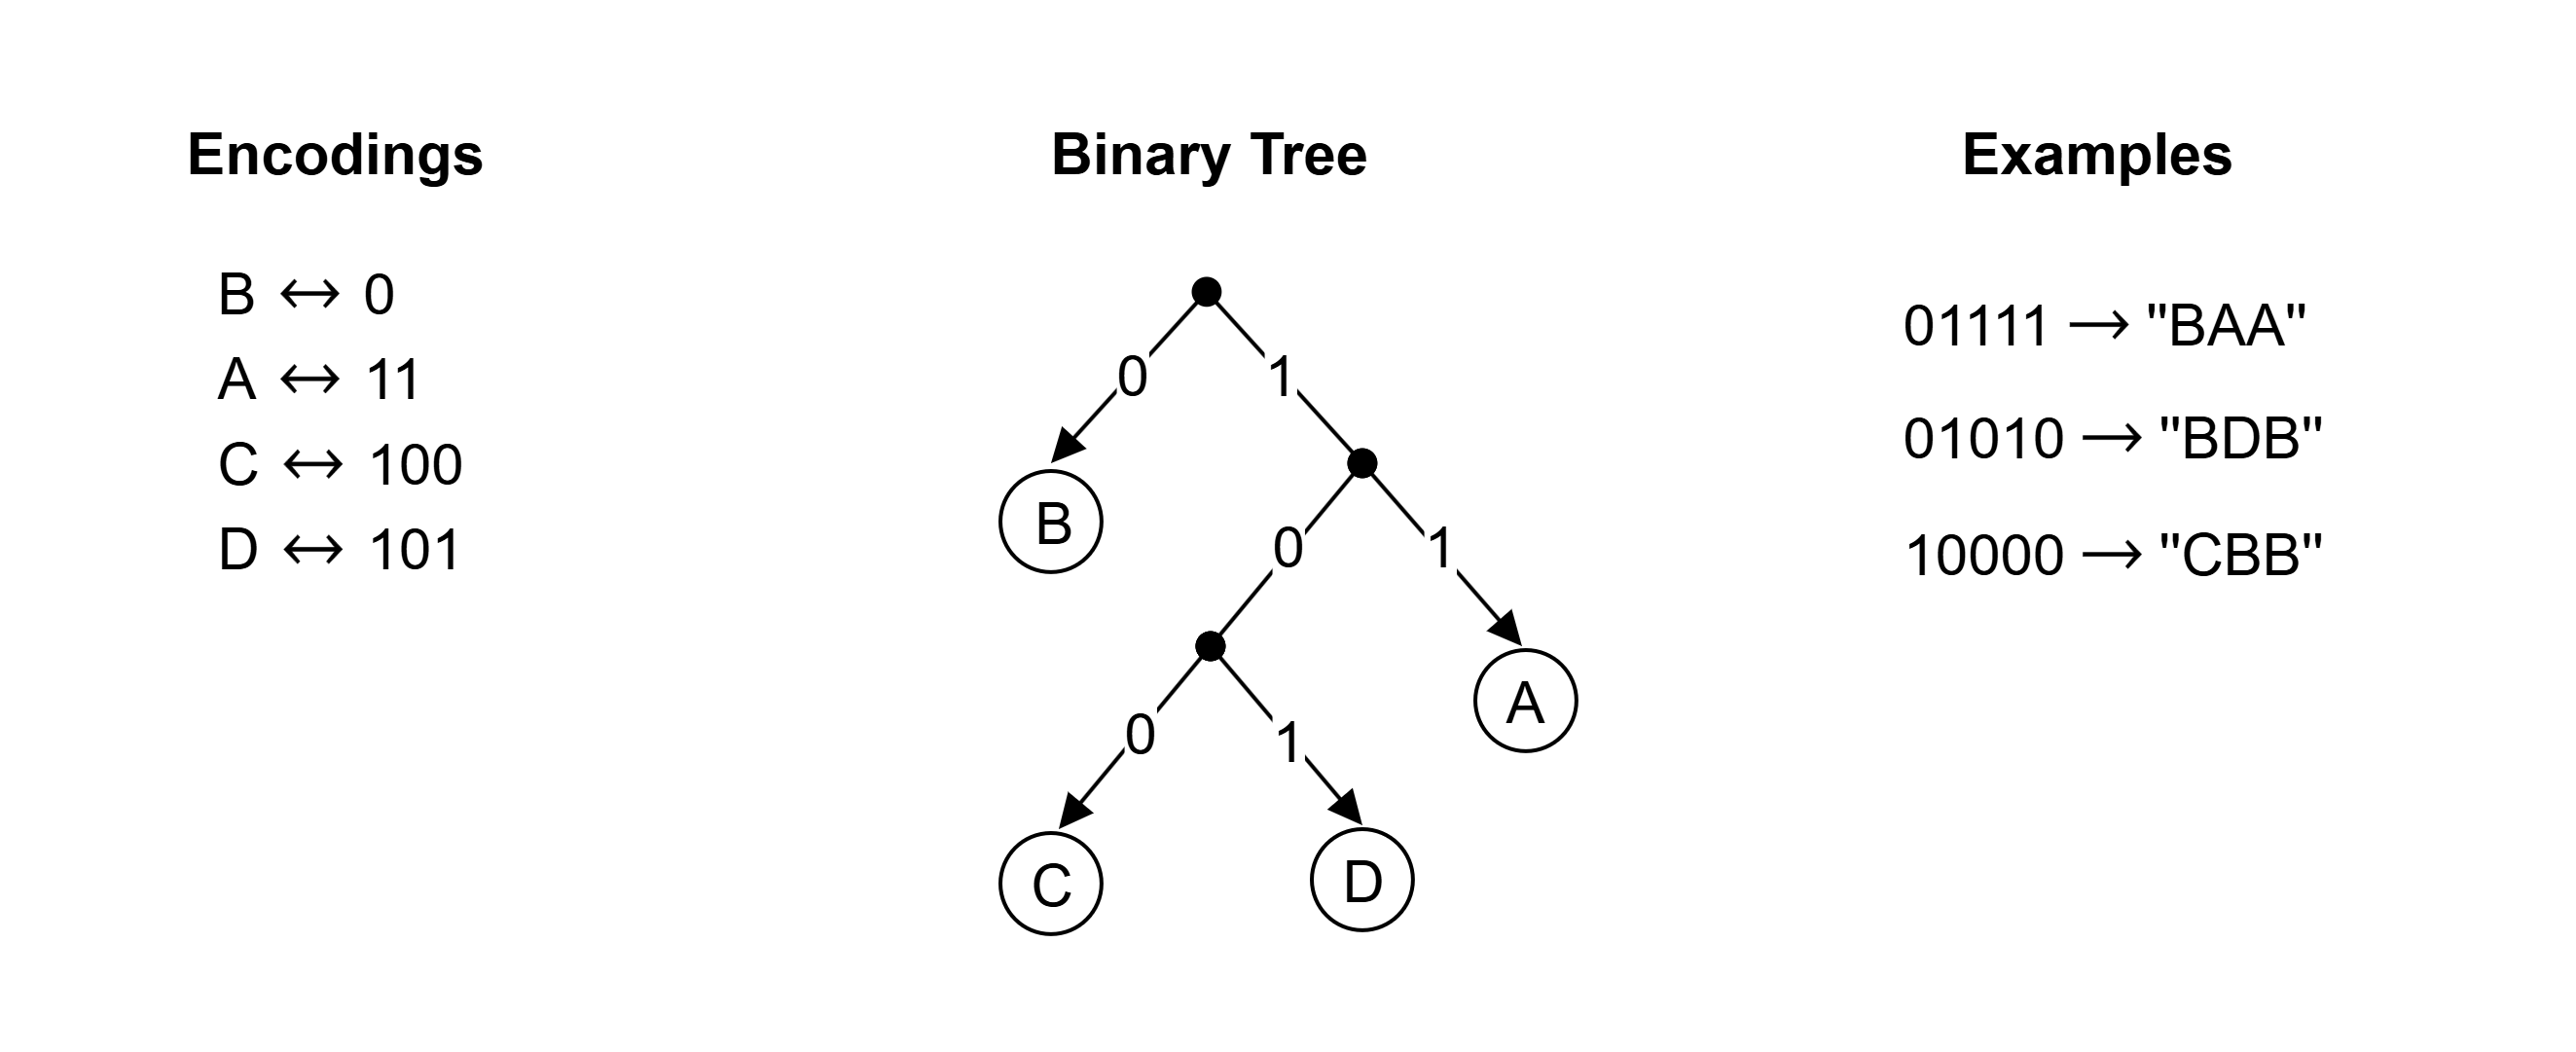
\includegraphics[width=\textwidth]{./Sections/comp/info/binary_tree_encoding.png}
    \caption{Encodings start at the root, each edge taken writes the next bit.}

    \label{fig:binary_tree_encoding}
\end{figure}

\newpage 



\newpage 




% \section{Efficient Encodings}

\label{sec:info_effic}

Now that we are familiar with B
% \vspace{-2em}
\section{Number Base System Encodings}

\label{sec:base_encodings}
 
\noindent
We now explore how to represent our base two or any other base number in a fixed-length encoding.

% \begin{Def}[Turing Machine]

%     A \textbf{Turing Machine} is a theoretical computational model used to describe the capabilities of a general-purpose \textbf{computer}. It consists of an infinite tape (memory) and a read/write head processing symbols on the tape, one at a time, according to a set of predefined rules. The machine moves left or right, reading or writing symbols, and changing states based on what it reads. 
    
%     The machine \textbf{halts} once it reaches a final state or continues indefinitely. Serving as a flexible, \textbf{higher-order function} (a function which receives functions).
% \end{Def}

\begin{Def}[Number Base Fixed-length Encoding]

    \label{def:number_base_fixed_length_encoding}

    \noindent
    Each memory cell in the computers stack is an integer value represented in a fixed base, typically \(B = 2\), 
    meaning \textbf{binary}. Where each digit is less than the base \(B\). We represent integers in memory as:

    \[
    a = \sum_{i=0}^{k-1} a_i B^i
    \]
    
    \noindent
    Where \( a_i \) represents the individual digits, and \(B\) is the base. For large integers, computations may require manipulating several memory cells to store the full number.
\end{Def}

\noindent
\begin{Example}[Binary \& Decimal Representations] 

Consider the integer, $a = 13$, in base, $B := 2$ \textbf{(binary)}, using Definition \ref{def:number_base_fixed_length_encoding}:

\Large
\[
a = \underbracket{(\text{\textcolor{red}{1}} \cdot 2^3) + (\text{\textcolor{red}{1}} \cdot 2^2) + (\text{\textcolor{red}{0}} \cdot 2^1) + (\text{\textcolor{red}{1}} \cdot 2^0)}_{\text{binary: \textcolor{red}{1101}}} = 8 + 4 + 0 + 1 = 13
\]
\normalsize

\vspace{1em}
\noindent
Here, the coefficients $a_3 = 1$, $a_2 = 1$, $a_1 = 0$, and $a_0 = 1$ correspond to the binary digits of $13$, where each 
power of $2$ represents the binary place value. Similarly, if we want to represent, $a = 45$, in base, \textbf{$B := 10$ (decimal)}:

\[
a = 4 \cdot 10^1 + 5 \cdot 10^0 = 40 + 5 = 45
\]

\noindent
In this case, the coefficients $a_1 = 4$ and $a_0 = 5$ correspond to the decimal digits of $45$.
\end{Example}

\noindent
We continue to common bases that one may encounter in computing and mathematics:
\begin{Def}[Hexadecimal]
    \textbf{Hexadecimal} base $B=16$, using digits 0-9 and the letters A-F, where:
    \begin{center}
        $A=10$, $B=11$, $C=12$, $D=13$, $E=14$, and $F=15$.
    \end{center} Hexadecimal is commonly used in computing due to its compact representation of binary data. E.g., 
    A \underline{\textbf{byte} (8 bits)} can be represented as two hexadecimal digits, simplifying the display of binary data.
\end{Def}

\newpage

\begin{theo}[Base $2\leftrightarrow16$ Conversion]

    Let bases \( B:=2 \) (binary) and \( H:=16 \) (hexadecimal). At a high-level:

    \vspace{.5em}
    
    \noindent \textbf{Binary to Hexadecimal:}
    \begin{enumerate}
        \item Group $B$ digits in sets of 4, right to left. \textbf{Pad} leftmost group with 0's if necessary for a full group.
        \item Compute each group, replacing the result with their $H$ digit.
        \item Finally, combine each $H$ group.
    \end{enumerate}
    
    \noindent \textbf{Hexadecimal to Binary:}
    \begin{enumerate}
        \item Convert each $H$ digit into a 4 bit $B$ group.
        \item Finally, combine all $B$ groups.
    \end{enumerate}
    \noindent
    Additionally, we may also trim any leading 0's.
\end{theo}

\noindent
\begin{Example}[Base $2\leftrightarrow16$ Conversion]
    \begin{itemize}
        \item Binary to Hexadecimal:
        \[
        101101111010_2 \quad \Rightarrow \quad \text{Group as } (\underbracket{[1011]}_{11} \ \underbracket{[0111]}_{7} \ \underbracket{[1010]}_{10}) \quad \Rightarrow \quad B7A_{16}
        \]
        \item Hexadecimal to Binary:
        \[
        3F5_{16} \quad \Rightarrow \quad [0011]\ [1111]\ [0101]_2 \Rightarrow \quad 1111110101_2
        \]
        \noindent
    \end{itemize}

\end{Example}

\noindent
The following definition is for completeness: applications of such a base are currently seldom.
\begin{Def}[Unary]
    
    \textbf{Unary}, base $B=1$. A system where each number is represented by a sequence of the same symbol. 
    This system is more theoretical than practical given today's systems.\\

    \noindent
    Given a toy unary system, we may represent numbers with a single symbol ``I'': $5 = \texttt{IIIII}$ or $2= \texttt{II}$. 
    The absence of symbols may represent 0.
\end{Def}

\begin{Def}[Most \& Least Significant Bit]
    
    In a binary number, the \textbf{most significant bit (MSB)} is the leftmost bit. The \textbf{least significant bit (LSB)} is the rightmost bit.\\

    \noindent
    E.g., In the byte (8 bits), $[1111 \ 1110]_2$, the MSB = 1 and the LSB = 0.
\end{Def}

\begin{theo}[Adding Binary]

    We may use the add and carry method alike decimal addition:\\

    \begin{minipage}{0.30\textwidth}
        \begin{itemize}
            \item $0 + 0 = 0$
            \item $0 + 1 = 1$
        \end{itemize}
    \end{minipage}
    \hfill
    \begin{minipage}{0.58\textwidth}
        \begin{itemize}
            \item $1 + 0 = 1$
            \item $1 + 1 = 0 \quad (\text{add 1 to the next digit (left)})$
        \end{itemize}
    \end{minipage}

    \vspace{1em}
    \noindent
    We call the last step a \textbf{carry}, as we carry our overflow to the next digit.
\end{theo}

\begin{Example}[Binary Addition]
    
\noindent   
Adding $0010\ 0011\ 0100_2$ and $0100_2$:
    \begin{equation*}
        \begin{array}{B3}
             1       &                             1000 &  \carry 0\textcolor{red}{1}00 \\
              {} + 0 &                             0001 &  0\textcolor{red}{1}00 \\ \hline
                   1 &                             1001 &  1000 \\
        \end{array}
        \end{equation*}
\noindent
Where $[1\ 1000\ 0100]_2 + [0\ 0001\ 0100]_2 = [1\ 1001\ 1000]_2$.
\end{Example}

\begin{Def}[Signed Binary Numbers - Two's Complement]
    
    In a \textbf{two's complement system}, an $n$-bit signed (positive or negative) binary number can represent values in the range $[-2^{n-1}, 2^{n-1}-1]$. Then by most significant bit (MSB):
    \begin{itemize}
        \item If MSB is 0, the number is positive;
        \item If MSB is 1, the number is negative.
    \end{itemize}
    \noindent
    \textbf{Conversion to Two's Complement :}
    \begin{enumerate}
        \item Take an unsigned binary number and invert all bits, turning 0's to 1's and 1's to 0's.
        \item Finally add 1 to the least significant bit.
    \end{enumerate}
\end{Def}

\begin{Example}[Two's Complement Conversion]
    
    \noindent
    Converting $-5$ into a 4-bit two's complement:
    \begin{align*}
        5 \rightarrow 0101 \quad & \text{(binary for 5)} \\
         1010 \quad & \text{(inverted)} \\
         1011 \quad & \text{(add 1)}
    \end{align*}
    Thus, $-5$ is represented as $1011$ in 4-bits under two's complement.
\end{Example}

\begin{Def}[Big \& Little Endian]
    
    \textbf{Big Endian} and \textbf{Little Endian} are two ways of storing multi-byte data in memory:
    \begin{itemize}
        \item \textbf{Big Endian:} The most significant byte (MSB) is stored at the lowest memory address 
        (How English reads and writes).
        \item \textbf{Little Endian:} The least significant byte (LSB) is stored at the lowest memory address.
    \end{itemize}

    \noindent
    Subsequent bytes are stored in increasing order. \textbf{Note:} A single byte has no endianness.
\end{Def}

\begin{figure}[ht!]
    \centering
    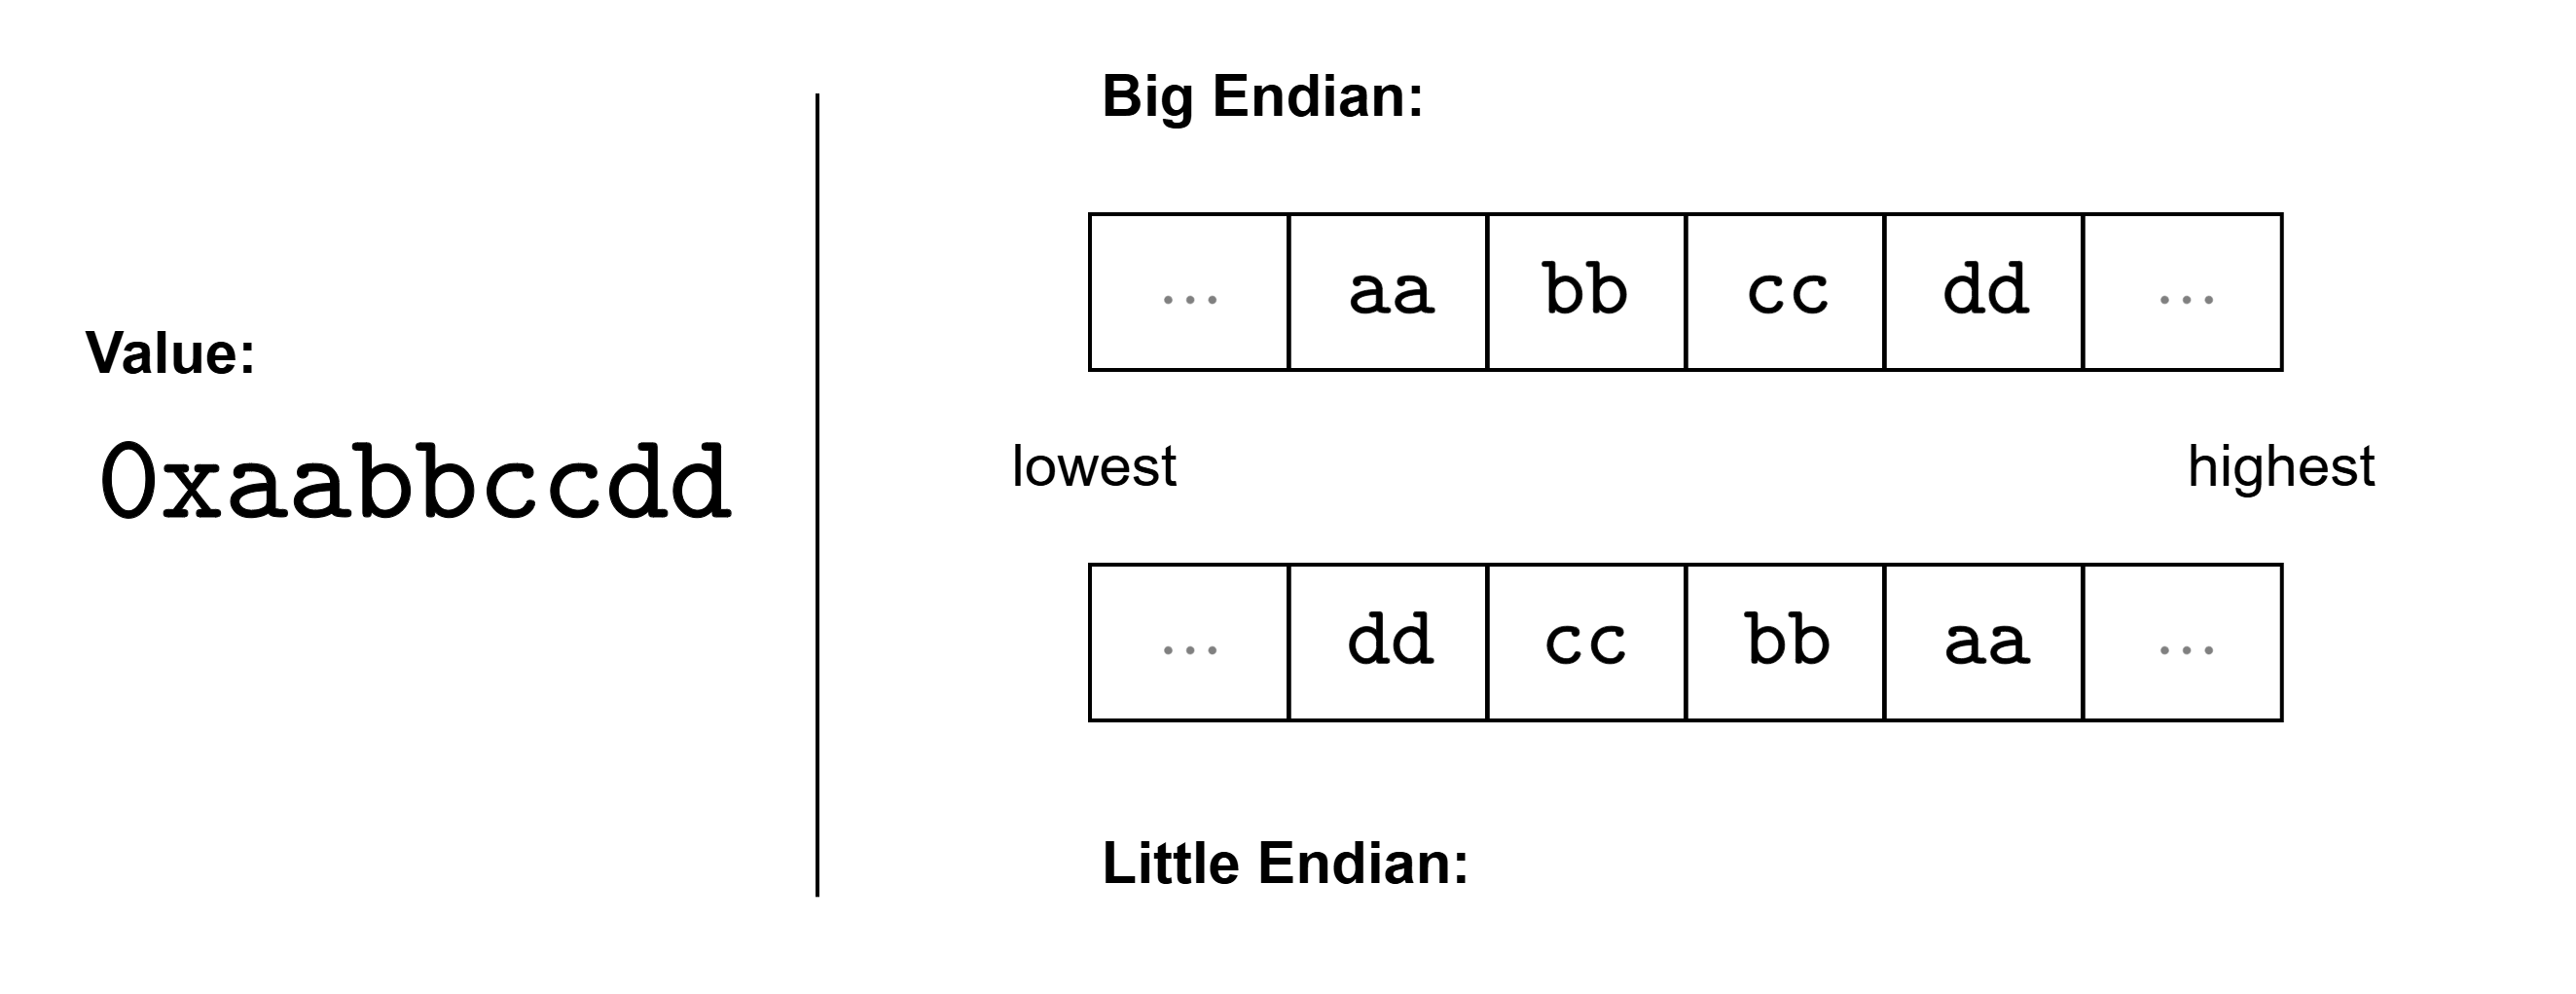
\includegraphics[width=0.8\textwidth]{sections/comp/big_endian.png}
    \caption{Big Endian vs Little Endian Representation of $0xaabbccdd$. Recall that $0x$ denotes a hexadecimal number,
    and $aa$ is a whole byte (8 bits) in hexadecimal.}
\end{figure}

\begin{Tip} The name ``endian'' comes from \emph{Gulliver's Travels} by Jonathan Swift, where
    Gulliver encounters two factions of people while traveling to the island of Lilliput. 
    One faction, the \textbf{Big-Endian}, believes that eggs should be cracked at the big end, 
    while the other faction, the \textbf{Little-Endian}, believes that eggs should be cracked at the little end.
\end{Tip}

    
\newpage

\begin{theo}[Commincation \& Endianess]

    \label{theo:communication_endianess}

    When communicating between systems, it is crucial to agree on the endianness of the data being sent. 
    If one system uses big-endian and the other uses little-endian, the data will be misinterpreted. 
    E.g., According to \href{https://datatracker.ietf.org/doc/html/rfc793}{RFC 793}, all the fields in network 
    headers must be big-endian.\\

    \noindent
    \rule{\textwidth}{0.4pt}\\
    \noindent
    \textbf{Note:} When debugging one might encounter an issue with endianness. Suppose we read the little-endian value
    $0xaabbccdd$ two bytes at a time. This gives us $A_1 = 0xccdd$ and $A_2 = 0xaabb$. The computer read both values 
    $B_1 = ddcc$ and $B_2 = bbaa$, translating it before sending it back to the debugger. This can cause issues as this is far beyond 
    the original value.
\end{theo}
% \section{Computing Large Numbers}
\noindent
In this section we discuss algorithms for computing large numbers, but first we define 
algorithmically, addition, subtraction, multiplication, division, and modula.

\begin{Def}[Wordsize]

    Our machine has a fixed \textbf{wordsize}, which is how much each memory cell can hold. Systems like 32-bit or 64-bit can hold $2^{32}$ $(\approx$ 4.3 billion) or $2^{64}$ $(\approx$ 18.4 quintillion) bits respectively.\\

    \noindent
    We say the ALU can performs arithmetic operations at $O(1)$ time, within wordsize. Operations beyond this size we deem \textbf{large numbers}.
\end{Def}
\noindent
The game we play in the following algorithms is to compute large integers without exceeding wordsize. Moving forward, we assume our machine is a typical 64-bit system.
\begin{Func}[Length of digits - $\|a\|$]

    We will use the notation $\|a\|$ to denote the number of digits in the integer $a$. For example, $\|123\| = 3$ and $\|0\| = 1$.
\end{Func}

\newpage
\begin{Def}[Computer Integer Division]

    Our ALU  \underline{only returns the quotient after division.} We denote the quotient as $\floor*{a/b}:a,b\in\Z$.
\end{Def}

\noindent
Our first hurdle is long division as , which will set up long addition and subtraction for success.

\noindent
\textbf{Scenerio - Grade School Long Division:} Goes as follows, take $\frac{a}{b}$. Find how times $b$ fits into $a$ evenly, $q$ times. Then $a-bq$ is our remainder $r$.\\
\textbf{Examples:} let $a=\{12,5,17,40,89\}$, $b=\{4,2,3,9,10\}$ respectively, and base $B=10$,
\begin{center}
    (1.)\intlongdivision{12}{4} (2.)\intlongdivision{5}{2} (3.)\intlongdivision{17}{3} (4.)\intlongdivision{40}{9} (5.)\intlongdivision{89}{10} 
\end{center}
\noindent
Take (3.), $a=17$, $b=3$: 3 fits into 17 five times, which is 15. 17 take away 15 is 2, our remainder. We 
create an algorithm to compute this process.\\

\noindent
\textbf{Key Observation:} Consider the following powers of 2 of form $x=2^n+s$, where $x,n,s\in\Z$:
\begin{align*}
    3 = 2 + 1 &= 0000 \ 00\textcolor{red}{11}_2 \quad (1) \\
    6 = 4 + 2 &= 0000 \ 0\textcolor{red}{11}0_2 \quad (2) \\
    12 = 8 + 4 &= 0000 \ \textcolor{red}{11}00_2 \quad (3) \\
    24 = 16 + 8 &= 000\textcolor{red}{1} \ \textcolor{red}{1}000_2 \quad (4) \\
    48 = 32 + 16 &= 00\textcolor{red}{11} \ 0000_2 \quad (5) \\
    96 = 64 + 32 &= 0\textcolor{red}{11}0 \ 0000_2 \quad (6) \\
    192 = 128 + 64 &= \textcolor{red}{11}00 \ 0000_2 \quad (7)
\end{align*}

\noindent
Notice that as we increase the power of 2, the number of bits shift left towards a higher-order bit. Now, instead of calculating powers of 
2, we shift bits left or right, to yield instantaneous results.

\begin{theo}[Binary Bit Shifting (Powers of 2)]

    \label{theo:bit_shift}

    Let $x$ be a binary unsigned integer. Where ``$\ll$'' and ``$\gg$'' are left and right bit shifts:\\
    \noindent
    \textbf{Left Shift by $k$ bits:} $x \ll k:= x \cdot 2^k$\\
    \noindent
    \textbf{Right Shift by $k$ bits:} $x \gg k = \left\lfloor x/2^k \right\rfloor$\\
    \textbf{Remainder:} bits pushed out after right shift(s).
\end{theo}

\newpage
\noindent
\textbf{Example:} Observe, $16=10000$ (4 zeros), $8=1000$ (3 zeros), we shift by 4 and 3 respectively:
\begin{itemize}
    \item Instead of $3 \cdot 16$ in base 10, we can $3 \ll 4=48$, as $3 \cdot 2^4 = 48$.
    \item Conversely, Instead of $48/16$ in base 10, $48 \gg 4 = 3$, as $\floor*{48/2^4} = 3$.
    \item Catching the remainder: say we have $37/8$ base 10, then,
        \[ 37 = 100101_2 \quad \text{and} \quad 8 = 1000_2 \text{ then } 37 \gg 3 = 4 \text{ remainder } 5,\]

    \noindent    
    as  $[100101]$ $\gg$ 3 = [000100]101, where $101_2$ is our remainder $5_{10}$.
\end{itemize}

\begin{Func}[Division with Remainder in Binary- \textit{QuoRem()}]

    \label{func:QuoRem}

    For binary integers, let dividend $a = (a_{k-1} \cdots a_0)_2$ and divisor $b = (b_{\ell-1} \cdots b_0)_2$ be unsigned, with $k \geq 1$,
    $\ell \geq 1$, ensuring $0 \leq b \leq a$, and $b_{\ell-1} \neq 0$, ensuring $b > 0$.\\ 
    
    \noindent
    We compute $q$ and $r$ such that, $a = bq + r$ and $0 \leq r < b$. 
    Assume $k \geq \ell$; otherwise, $a < b$. We set $q \gets 0$ and $r \gets a$. 
    Then quotient $q = (q_{m-1} \cdots q_0)_2$ where $m := k - \ell + 1$.\\

    \noindent
    \textbf{Input:} $a, b$ (binary integers)\\
    \noindent
    \textbf{Output:} $q, r$ (quotient and remainder in binary)\\
    \begin{algorithm}[H]
        \SetAlgoLined
        \SetKwProg{Fn}{Function}{:}{\KwRet{$(q, r)$;}}
        \Fn{\textit{QuoRem}($a, b$)}{
            $r \gets a$\;
            $q \gets \{0_{m-1} \cdots 0\}$\;
            \vspace{.5em}
            \For{$i \gets \|a\|-\|b\|-1$ $\textbf{\text{down to}}$ $0$}{
                $q_i \gets \left\lfloor \dfrac{r}{b \ll i} \right\rfloor$\; 
                $r \gets r - (q_i \cdot (b \ll i))$\;  
            }
          
        }
    \end{algorithm}
    \noindent\rule{\textwidth}{0.4pt}
    \noindent

    \noindent
    \textbf{Time Complexity}: $O(\|a\|(\|a\| - \|b\|))$. In short, line 5 we preform division on $\|a\|$ bits of decreasing size.
    For more
    detail visit \url{https://shoup.net/ntb/ntb-v2.pdf} on page 60. \textbf{I would not} stare at this too
    long. General $n$ cases can be found in Theorem (\ref{theo:basic-arithmetic}).
\end{Func}

\noindent
\textbf{Example} Let $a = 47_{10} = 101111_2$ and $b = 5_{10} = 101_2$, we run \textit{QuoRem($a,b$)}. We summarize the above example as, ``How many times does $101_2$ fit into $101111_2$?''
\begin{enumerate}
    \item  Does $5\ll 3$ fit into $101000_2$? It fits! $q=1000_2$, $r = 101111_2 - 101000_2$.
    \item  Does $5\ll 2$ fit into $0111_2$? no fits! $q=1000_2$, $r = 0111_2$.
    \item  Does $5\ll 1$ fit into $0111_2$? no fits! $q=1000_2$, $r = 0111_2$.
    \item  Does $5\ll 0$ fit into $0111_2$? It fits! $q=1001_2$, $r = 0111_2-0101$.
    \item  Return $q=1001_2=9_{10}$, $r = 0010 = 2_{10}$ 
\end{enumerate}

\newpage



\noindent
Long addition: We craft an algorithm for
grade school long addition, which goes as follows:
\begin{equation*}
    \begin{array}{@{}B2}
        \carry 2 5 & 3\carry 0  8 \\
                 {} + 39 &                  406 \\ \hline
                      64 &                  714 \\
    \end{array}
    \end{equation*}
\noindent
Where adding, $25,308 + 39,406 = 64,714$. We create an algorithm to compute this in the following function.\\

\noindent
Here the function $QuoRem$ (\ref{func:QuoRem}) to return (quotient, remainder) preforms in $O(1)$ as bits are small enough for word size.
\begin{Func}[Addition of Binary Integers - \textit{Add()}]
    Let $a = (a_{k-1} \cdots a_0)_2$ and $b = (b_{\ell-1} \cdots b_0)_2$ be unsigned binary integers, where $k \geq \ell \geq 1$. We compute $c := a + b$ where the result $c = (c_{k}c_{k-1} \cdots c_0)_2$ is of length $k+1$, assuming $k \geq \ell$. If $k < \ell$, swap $a$ and $b$. This algorithm computes the binary representation of $a + b$.

    \vspace{.5em}
    \noindent
    \textbf{Input:} $a, b$ (binary integers)\\
    \textbf{Output:} $c = (c_k \cdots c_0)_2$ (sum of $a + b$)\\

    \begin{algorithm}[H]
        \SetAlgoLined
        \SetKwProg{Fn}{Function}{:}{\KwRet{}}
        \Fn{\textit{Add}($a, b$)}{
            $carry \gets 0$\;
            \For{$i \gets 0$ \textbf{to} $\ell - 1$}{
                $tmp \gets a_i + b_i + carry$\;
                $(carry, c_i) \gets \texttt{QuoRem}(tmp, 2)$\;
            }
            \For{$i \gets \ell$ \textbf{to} $k - 1$}{
                $tmp \gets a_i + carry$\;
                $(carry, c_i) \gets \texttt{QuoRem}(tmp, 2)$\;
            }
            $c_k \gets carry$\;
            \KwRet{$c = (c_k \cdots c_0)_2$}\;
        }
    \end{algorithm}
    \noindent\rule{\textwidth}{0.4pt}

    \noindent
    \textbf{Note:} $0 \leq \textit{carry} \leq 1$ and $0 \leq \textit{tmp} \leq 3$.\\
    \textbf{Time Complexity:} $O(\max(\|a\|,\|b\|))$, as we iterate at most the length of the largest input.\\
    \textbf{Space Complexity:} $O(\|a\|+\|b\|)$, though $c = k+1$, constants are negligible as $k, \ell \to \infty$.
\end{Func}

\newpage

\noindent
For subtracting, $5,308 - 3,406 = 1,904$, where we borrow 10 from the 5 to make 13:
\begin{equation*}
    \begin{array}{@{}B2}
         \not{\carry[4]5} & \carry[10] 3 0  8 \\
                 {} - 3 &                  406 \\ \hline
                      1 &                  904 \\
    \end{array}
\end{equation*}

\vspace{-1em}
\begin{Func}[Subtraction of Binary Integers - \textit{Subtract()}]
    Let \( a = (a_{k-1} \cdots a_0)_2 \) and \( b = (b_{\ell-1} \cdots b_0)_2 \) be unsigned binary integers, where \( k \geq \ell \geq 1 \) and \( a \geq b \). We compute \( c := a - b \) where the result \( c = (c_{k-1} \cdots c_0)_2 \) is of length \( k \), assuming \( a \geq b \). If \( a < b \), swap \( a \) and \( b \) and set a negative flag to indicate the result is negative. This algorithm computes the binary representation of \( a - b \).
    
    \vspace{.5em}
    \noindent
    \textbf{Input:} \( a, b \) (binary integers)\\
    \textbf{Output:} \( c = (c_{k-1} \cdots c_0)_2 \) (difference of \( a - b \))
    
    \begin{algorithm}[H]
        \SetAlgoLined
        \SetKwProg{Fn}{Function}{:}{\KwRet{}}
        \Fn{\textit{Subtract}($a, b$)}{
            $borrow \gets 0$\;
            \For{$i \gets 0$ \textbf{to} $\ell - 1$}{
                $tmp \gets a_i - b_i - borrow$\;
                \eIf{$tmp < 0$}{
                    $borrow \gets 1$\;
                    $c_i \gets tmp + 2$\;
                }{
                    $borrow \gets 0$\;
                    $c_i \gets tmp$\;
                }
            }
            \For{$i \gets \ell$ \textbf{to} $k - 1$}{
                $tmp \gets a_i - borrow$\;
                \eIf{$tmp < 0$}{
                    $borrow \gets 1$\;
                    $c_i \gets tmp + 2$\;
                }{
                    $borrow \gets 0$\;
                    $c_i \gets tmp$\;
                }
            }
            \KwRet{$c = (c_{k-1} \cdots c_0)_2$}\;
        }
    \end{algorithm}
\noindent\rule{\textwidth}{0.4pt}

\noindent
\textbf{Note:} $0\leq borrow\leq 1$. Subtraction may produce a borrow when $a_i < b_i$.\\
\textbf{Time Complexity:} \( O(\max(\|a\|, \|b\|)) \), iterating at most the length of the largest input.\\
\textbf{Space Complexity:} \( O(\|a\| + \|b\|) \), as the length of \( c \) is at most \( k \), with constants negligible as \( k, \ell \to \infty \).
\end{Func}
    


\newpage

\noindent
For multiplication, $24\cdot 16= 384$:
\begin{equation*}
    \begin{array}{@{}B2}
                                            &  \carry[2]24 \\
                 {} \times  &                  16 \\ \hline
                 {}   &                  144 \\ 
                 {} +  &                  240 \\ \hline
                       &                  384 \\
    \end{array}
\end{equation*}
\noindent
Where $6\cdot 4 = 24$, we write the 4 and carry the 2. Then $6\cdot 2 = 12$ plus the carried 2 is 14. Then we multiply the next digit, 1, we add a 0 below our 144, and repeat the process. Every new 10s place we add a 0. Then we add our two products to get 384.\\

\noindent
We create an algorithm to compute this process in the following function:
\begin{Func}[Multiplication of Base-$B$ Integers - \textit{Mul()}]
    \label{func:mul}
    Let $a = (a_{k-1} \cdots a_0)_B$ and $b = (b_{\ell-1} \cdots b_0)_B$ be unsigned integers, where $k \geq 1$ and $\ell \geq 1$. The product $c := a \cdot b$ is of the form $(c_{k+\ell-1} \cdots c_0)_B$, and may be computed in time $O(k\ell)$ as follows:

    \vspace{.5em}
    \noindent
    \textbf{Input:} $a, b$ (base-$B$ integers)\\
    \textbf{Output:} $c = (c_{k+\ell-1} \cdots c_0)_B$ (product of $a \cdot b$)\\

    \begin{algorithm}[H]
        \SetAlgoLined
        \SetKwProg{Fn}{Function}{:}{\KwRet{}}
        \Fn{\textit{Mul}($a, b$)}{
            \For{$i \gets 0$ \textbf{to} $k + \ell - 1$}{
                $c_i \gets 0$\;
            }
            \For{$i \gets 0$ \textbf{to} $k - 1$}{
                $carry \gets 0$\;
                \For{$j \gets 0$ \textbf{to} $\ell - 1$}{
                    $tmp \gets a_i \cdot b_j + c_{i+j} + carry$\;
                    $(carry, c_{i+j}) \gets \texttt{QuoRem}(tmp, B)$\;
                }
                $c_{i+\ell} \gets carry$\;
            }
            \KwRet{$c = (c_{k+\ell-1} \cdots c_0)_B$}\;
        }
    \end{algorithm}

    \noindent\rule{\textwidth}{0.4pt}
    
    \noindent
    \textbf{Note:} At every step, the value of \textit{carry} lies between $0$ and $B-1$, and the value of \textit{tmp} lies between $0$ and $B^2 - 1$.\\
    \textbf{Time Complexity:} $O(\|a\|\cdot\|b\|)$, since the algorithm involves $k \cdot \ell$ multiplications.\\
    \textbf{Space Complexity:} $O(\|a\| + \|b\|)$, since we store the digits of $a$, $b$, and $c$.
\end{Func}



\newpage
\begin{Func}[Decimal to Binary Conversion - \textit{DecToBin()}]
    This function converts a decimal number $n$ into its binary equivalent by repeatedly dividing the decimal number by 2 and recording the remainders.

    \vspace{.5em}
    \noindent
    \textbf{Input:} $n$ (a decimal number)\\
    \textbf{Output:} $b$ (binary representation of $n$)\\

    \begin{algorithm}[H]
        \SetAlgoLined
        \SetKwProg{Fn}{Function}{:}{\KwRet{}}
        \Fn{\textit{DecToBin}($n$)}{
            $b \gets \text{empty string}$\;
            \While{$n > 0$}{
                $r \gets n \bmod 2$\;
                $n \gets \left\lfloor \frac{n}{2} \right\rfloor$\;
                $b \gets r \ + \ b$\; % Prepend the remainder to the binary string
            }
            \KwRet{$b$}\;
        }
    \end{algorithm}
    \noindent\rule{\textwidth}{0.4pt}
    
    \noindent
    \textbf{Time Complexity:} $O(\log n)$, as the number of iterations is proportional to the number of bits in $n$.\\
    \textbf{Space Complexity:} $O(n)$, storing our input $n$.
\end{Func}

\noindent
\textbf{Example:} Converting 89 to binary given the above function:
\begin{align*}
    89_{10} &\div 2 = 44 \quad \text{rem} \ 1, \longleftarrow \textbf{ LSB}&   \\
    44_{10} &\div 2 = 22 \quad \text{rem} \ 0,& \\
    22_{10} &\div 2 = 11 \quad \text{rem} \ 0,& \\
    11_{10} &\div 2 = 5 \quad \ \text{rem} \ 1,& \\
    5_{10} &\div 2 = 2 \quad \ \text{rem} \ 1,& \\
    2_{10} &\div 2 = 1 \quad \ \text{rem} \ 0,& \\
    1_{10} &\div 2 = 0 \quad \ \text{rem} \ 1.  \longleftarrow \textbf{ MSB} &  
\end{align*}
Thus, $89_{10} = 1011001_2$.

\begin{theo}[Time Complexity of Basic Arithmetic Operations]
    
    \label{theo:basic-arithmetic}

    We generalize the time complexity to $a$ and $b$ as $n$-bit integers. 
    \begin{enumerate}[(i)]
        \item \textbf{Addition \& Subtraction:} $a \pm b$ in time $O(n)$.
        \item \textbf{Multiplication:} $a \cdot b$ in time $O(n^2)$.
        \item \textbf{Quotient Remainder} quotient $q := \left\lfloor \frac{a}{b} \right\rfloor: b \neq 0, a>b;$ and remainder $r := a \mod b$ has time $O(n^2)$.
    \end{enumerate}
\end{theo}
% \section{Manipulating Numbers in Base 2}

\label{sec:effic}

\begin{theo}[Binary Length of a Number - $\|a\|$]
    
    The binary length of an integer $a_{10}$ in binary representation, is given by:
    
    \[
    \|a\| := 
    \begin{cases} 
    \lfloor \log_2 |a| \rfloor + 1 & \text{if } a \neq 0, \\
    1 & \text{if } a = 0,
    \end{cases}
    \]
    
    \noindent
    as $\lfloor \log_2 |a| \rfloor + 1$ correlates to the highest power of 2 required to represent $a$.
\end{theo}


\vspace{-1em}
\begin{Example}[Base 10 and Base 2 Lengths]

\label{ex:log_length}

\vspace{-1em}
Think of base 10 and a 9 digit number $d=684,301,739$.
To reach 9 digits takes $10^8$; The exponent plus 1 yields $\|d\|$. Hence, $\lfloor \log_{10} d\rfloor+1$ is $\|d\|$.
Now, let there be a 7 digit binary number $b=1001000$, which expanded is:

$$ (1\cdot 2^6) + (0\cdot 2^5) + (0\cdot 2^4) + (1\cdot 2^3) + (0\cdot 2^2) + (0\cdot 2^1) + (0\cdot 2^0) = 72,$$
\noindent
Taking $6$ powers of 2 to reach $72$, we add 1 to get $\|b\| = 7$. Hence, $\|b\| = \lfloor \log_2 b \rfloor + 1$.

\noindent
Additionally, if $a=0_2$ then $\|a\|=1$. as $a^0=1$.
\end{Example}


\vspace{-.5em}
\begin{theo}[Splitting Higher and Lower Bits]

    Let $a$ be a binary number with $n$ bits. We can split $a$ into two numbers $A_1$ and $A_0$ with $n/2$ bits each,
    representing the first and second halves respectively. Where:
    
        $$A_1:=\frac{a}{2^{\ceil{n/2}}} \quad \text{ and } \quad A_0:=a \text{ mod } 2^{\ceil{n/2}}$$

\end{theo}

\vspace{-1em}
\begin{Example}[Splitting \& Shifting Base 10 and 2]

\label{ex:split_base}

\vspace{-.5em}
Given $a=745,562,010_{10}$, we split it in half as follows:
\[ A_1=\frac{745,562,010}{10^{\ceil{9/2}}}=7455, \quad \text{ and } \quad A_0=745,562,010 \text{ mod } 10^{\ceil{9/2}}=62,010 \]
\noindent
We can use the same bit shifting technique from Theorem (\ref{theo:bit_shift}) for base 10:
$$[745,562,010]_{10} \text{ right shift by 5, } [000,007,455]_{10}\ 62,010.$$ 

\noindent
Given $[1111\ 1111\ 1001\ 1001_2]$ ($32665_{10}$), which is 16 bits long, we can split it in half, as follows:

\[ 
A_1=\frac{1111\ 1111\ 1001\ 1001_2}{2^{\ceil{16/2}}}=1111\ 1111_2
\]
\[A_0=1111\ 1111\ 1001\ 1001_2 \text{ mod } 2^{\ceil{16/2}}=1001\ 1001_2 \]

\vspace{-2em}
\end{Example}



\noindent




\chapter{Circuits and Logic}
\section{Representing Information}

\subsection{Electricity \& Information: Volts, Amps, \& Watts}
\label{sec:info}

\noindent
Figuring out how to represent information is tricky: Nature encodes information in DNA, though 
it may be hard to store because of decay (This is an active area of research). Punching holes 
in cards was a common method of storing information, but it's difficult to manipulate. Ideally:
\begin{itemize}
    \item \textbf{Inexpensive:} We want to reproduce at scale with low costs.
    \item \textbf{Stable:} Reliably store information for long periods.
    \item \textbf{Mutable:} The ability to manipulate information easily.
\end{itemize}

\begin{Def}[Electricity \& Information]

    \label{def:elec_info}

    Electricity is a flow of electrons, which can be used to represent information. 
    We can use the presence or absence of an electric current to represent binary values:
    \begin{itemize}
        \item \textbf{1} for presence of current;
        \item \textbf{0} for absence of current.
    \end{itemize}
    \noindent
    This is the basis of digital electronics and computing.
\end{Def}
\noindent
This is great for our applications, as electricity is relatively inexpensive given the scale of production.

\begin{theo}[Noise \& Error Accumulation]

    \label{theo:noise}

    We ought to keep in mind that electricity is not perfect. Though we design systems to measure information,
    slight inaccuracies or environmental factors may introduce noise, which over time corrupts information.
\end{theo}

\newpage 

\noindent
It's important that we understand the difference between analog and digital systems:
\begin{Def}[Analog vs. Digital]

    \label{def:analog_digital}

    An \textbf{analog} system is one that uses continuous signals to represent information, while a \textbf{digital} system uses discrete values (e.g., binary) to represent information.
\end{Def}

\begin{Example}[Real World Analog vs. Digital]

    \noindent
    Vinyl records are analog, as the grooves on the record represent sound waves continuously. 
    In contrast, a digital system would be a CD or MP3 file, where sound is represented as discrete samples of the original sound wave.
\end{Example}

\noindent
Our main focus will be on digital systems, representing the strength of electricity as binary values.
First we will briefly understand the terminology used in electrical systems:
\begin{Def}[Voltage, Amps, \& Watts]

    \label{def:voltage_amps_watts}

    Definition wise we have the following terms in electrical systems:
    \begin{itemize}
        \item \textbf{Voltage (Volts):} The potential difference between two points in an electrical circuit, measured in volts (V).
        \item \textbf{Amperage (Amps):} The flow of electric \textbf{current}, measured in amperes (A/$I$).
        \item \textbf{Resistance (Ohms):} The opposition to the flow of electric current, are ohms ($\Omega$/R).
        \item \textbf{Power (Watts):} The rate at which electrical energy is transferred, are watts (W).
    \end{itemize}

    \noindent
    We calculate all such as follows:
    \begin{itemize}
        \item \textbf{Voltage:} $V = I \cdot R$ (Voltage = Current $\times$ Resistance).
        \item \textbf{Current:} $I = P / V$ (Current = Power / Voltage).
        \item \textbf{Resistance:} $R = V / I$ (Resistance = Voltage / Current).
        \item \textbf{Power:} $P = V \cdot I$ (Power = Voltage $\times$ Current).
    \end{itemize}

    \noindent
    These ratios between Voltage, Current, and Resistance are part of \textbf{Ohm's Law}.
\end{Def}

\newpage 

\noindent
Let's understand this with a common analogy to water flow:

\begin{Example}[Water \& Electric Flow Analogy]

    \noindent
    Imagine a water pipe system:
    \begin{itemize}
        \item \textbf{Voltage} is the water pressure in the pipes, the force pushing water through the system.
        \item \textbf{Current} is the amount of water flowing through the pipes at any given time.
        \item \textbf{Resistance} is the size of the pipes, which affects how easily water can flow.
        \item \textbf{Power} is the total amount of water that flowed through the system over time.
    \end{itemize}
\end{Example}


\noindent
The relationship between Voltage, Current, and Resistance has a handy visualization:

\begin{Def}[Ohm's Triangle]

    \label{def:ohms_triangle}

    \noindent
    Ohm's Triangle is a visual representation of the relationship between Voltage, Current, and Resistance. 
    If any two values are known, the third can be calculated using the triangle:\\

\noindent
    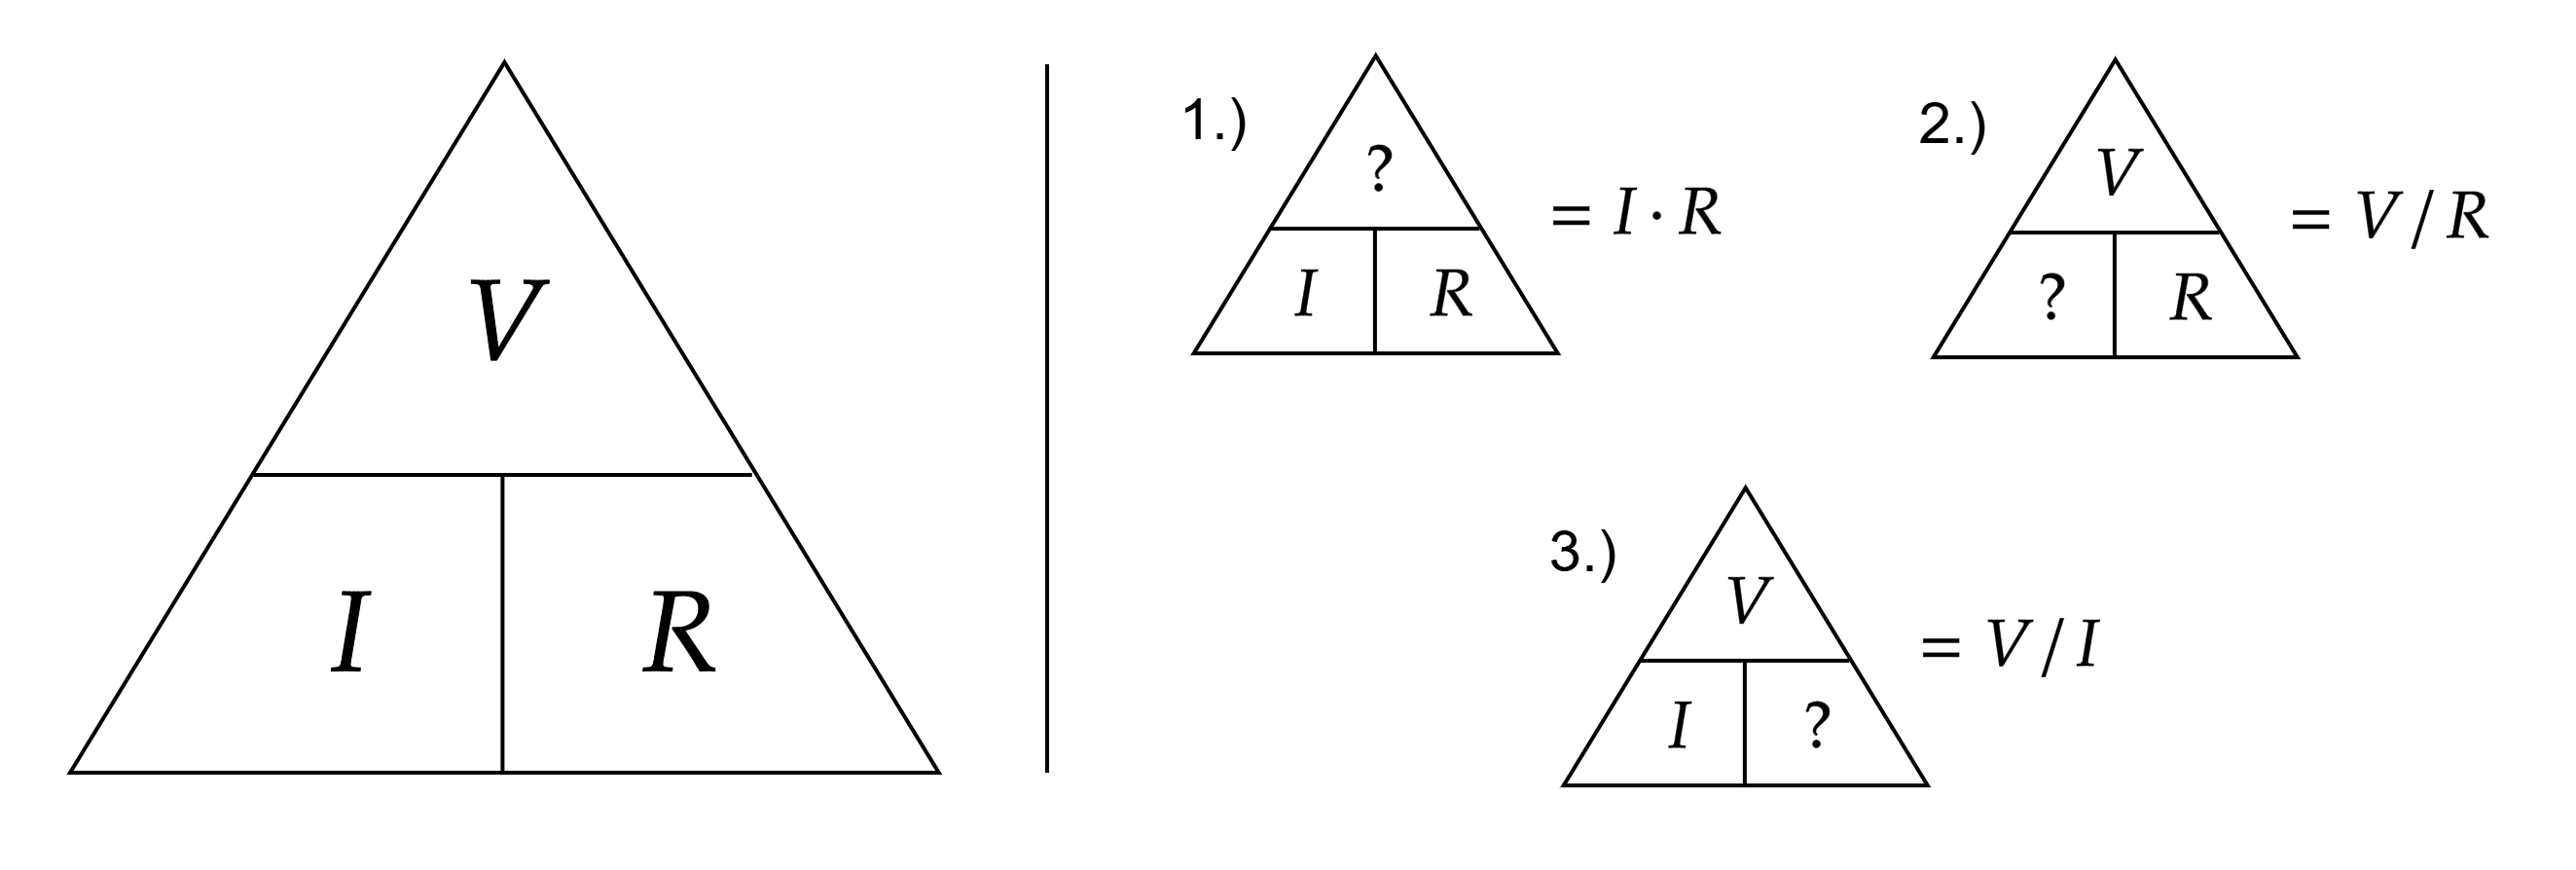
\includegraphics[width=\textwidth]{./Sections/circuits/triangle.png}

    \noindent
    Here, Voltage ($V$) is at the top, with Current ($I$) and Resistance ($R$) at the bottom corners:
    \begin{enumerate}
        \item \textbf{Voltage} is unknown: $V = I \cdot R$.
        \item \textbf{Current} is unknown: $I = V / R$.
        \item \textbf{Resistance} is unknown: $R = V / I$
    \end{enumerate}

    \noindent
    A common mnemonic to remember is ``Viral'' for VIR (Voltage, Current, Resistance).
\end{Def}

\newpage 

\noindent
Now for completeness sake, we distinguish the following:

\begin{Def}[Energy vs. Power]

    \label{def:energy_power}

    \noindent
    \textbf{Energy} is the capacity to do work, measured in joules (J). 
    \textbf{Power} is the rate at which work/energy is done or used, measured in watts (W).
    \noindent
    This is given by the formulation:
    \[
        P = E / t
    \]
    where $P$ is power, $E$ is energy, and $t$ is time.
\end{Def}

\noindent
\begin{Example}[Energy-Power Water Analogy]

    \noindent
    Continuing with the water analogy:
    \begin{itemize}
        \item \textbf{Energy} is the total amount of water stored in a tank.
        \item \textbf{Power} is how fast water flows out of the tank per second.
    \end{itemize}
    \noindent
    If we have a large tank (more energy), and water flows out slowly, we have high energy but low power. 
    Conversely, if we open the tap wide (high power), we use up the water quickly.

   
\end{Example}

\noindent
We will wrap up such with a final analogy that uses numbers:
 \begin{Example}[Mathematical Water Analogy]

        \begin{itemize}
            \item \textbf{Water Gun:} Imagine a water gun with very high pressure granted by
             the resistance of its small nozzle, so only a little water comes out.
            \begin{itemize}
                \item Pressure (Voltage) = 10 V
                \item Water Flow (Current) = 1 A
                \item Power = $10 \text{ V} \times 1 \text{ A} = 10 \text{ W}$
            \end{itemize}

            \item \textbf{Large Hose:} Now, consider a large fire hose with lower pressure but a much wider opening with 
            less resistance, allowing a lot of water to flow.
            \begin{itemize}
                \item Pressure (Voltage) = 2 V
                \item Water Flow (Current) = 5 A
                \item Power = $2 \text{ V} \times 5 \text{ A} = 10 \text{ W}$
            \end{itemize}
        \end{itemize}
        \noindent
        Both systems consumed the same amount of power (10 W), despite supporting different voltages, currents, and 
        possibly energy supplies. \textbf{Question:} What is the resistance of each system?

    \end{Example}

    \newpage 

    \subsection{Digitally Encoding Information}

    \label{sec:digitally_encoding}

    \noindent
    We now focus on representing information digitally:

    \begin{Def}[Digital Current Encoding Threshold]

        \label{def:digital_current_encoding_threshold}

        \noindent
        Given a line of voltage $V$, which we measure, $V_{TH}$ serves as a threshold:
        \[
         \text{0-bit} < V_{TH} < \text{1-bit}
        \]
        \noindent
        In practice, we have noise $\epsilon$ in our measurements, making it hard to 
        discern $V_{TH}+\epsilon$ from $V_{TH}-\epsilon$. To mitigate this, we
        pad the threshold from both sides called the \textbf{forbidden zone}:
        \[
        \text{0-bit} \leq V_{L} < \text{``Forbidden Zone''} < V_{H} \leq \text{1-bit}
        \]

        \noindent
        Where $V_L$ (low-level) and $V_H$ (high-level) are the region markers for valid voltage distinction.
    \end{Def}

    \vspace{-.5em}
    \begin{Def}[Combinational Device]

        \label{def:combinational_device}

        \noindent
        A \textbf{combinational device} is follows four specifications (spec.) called the, \textbf{static discipline}:

        \begin{itemize}
            \item \textbf{Input:} A set of input signals (i.e., measuring voltage levels).
            \item \textbf{Output:} A set of output signals (i.e., outputting voltage levels).
            \item \textbf{Functional Spec:} A mapping of all possible input combinations to an output value.
            \item \textbf{Timing Spec:} Detailing an upper bound $t_{PD}$ \textbf{(Propagation Delay)}, which is the minimum 
            amount of time needed for the output to stabilize on a new value after an input change.
        \end{itemize}
    \end{Def}

    \begin{figure}[ht!]

        \centering
        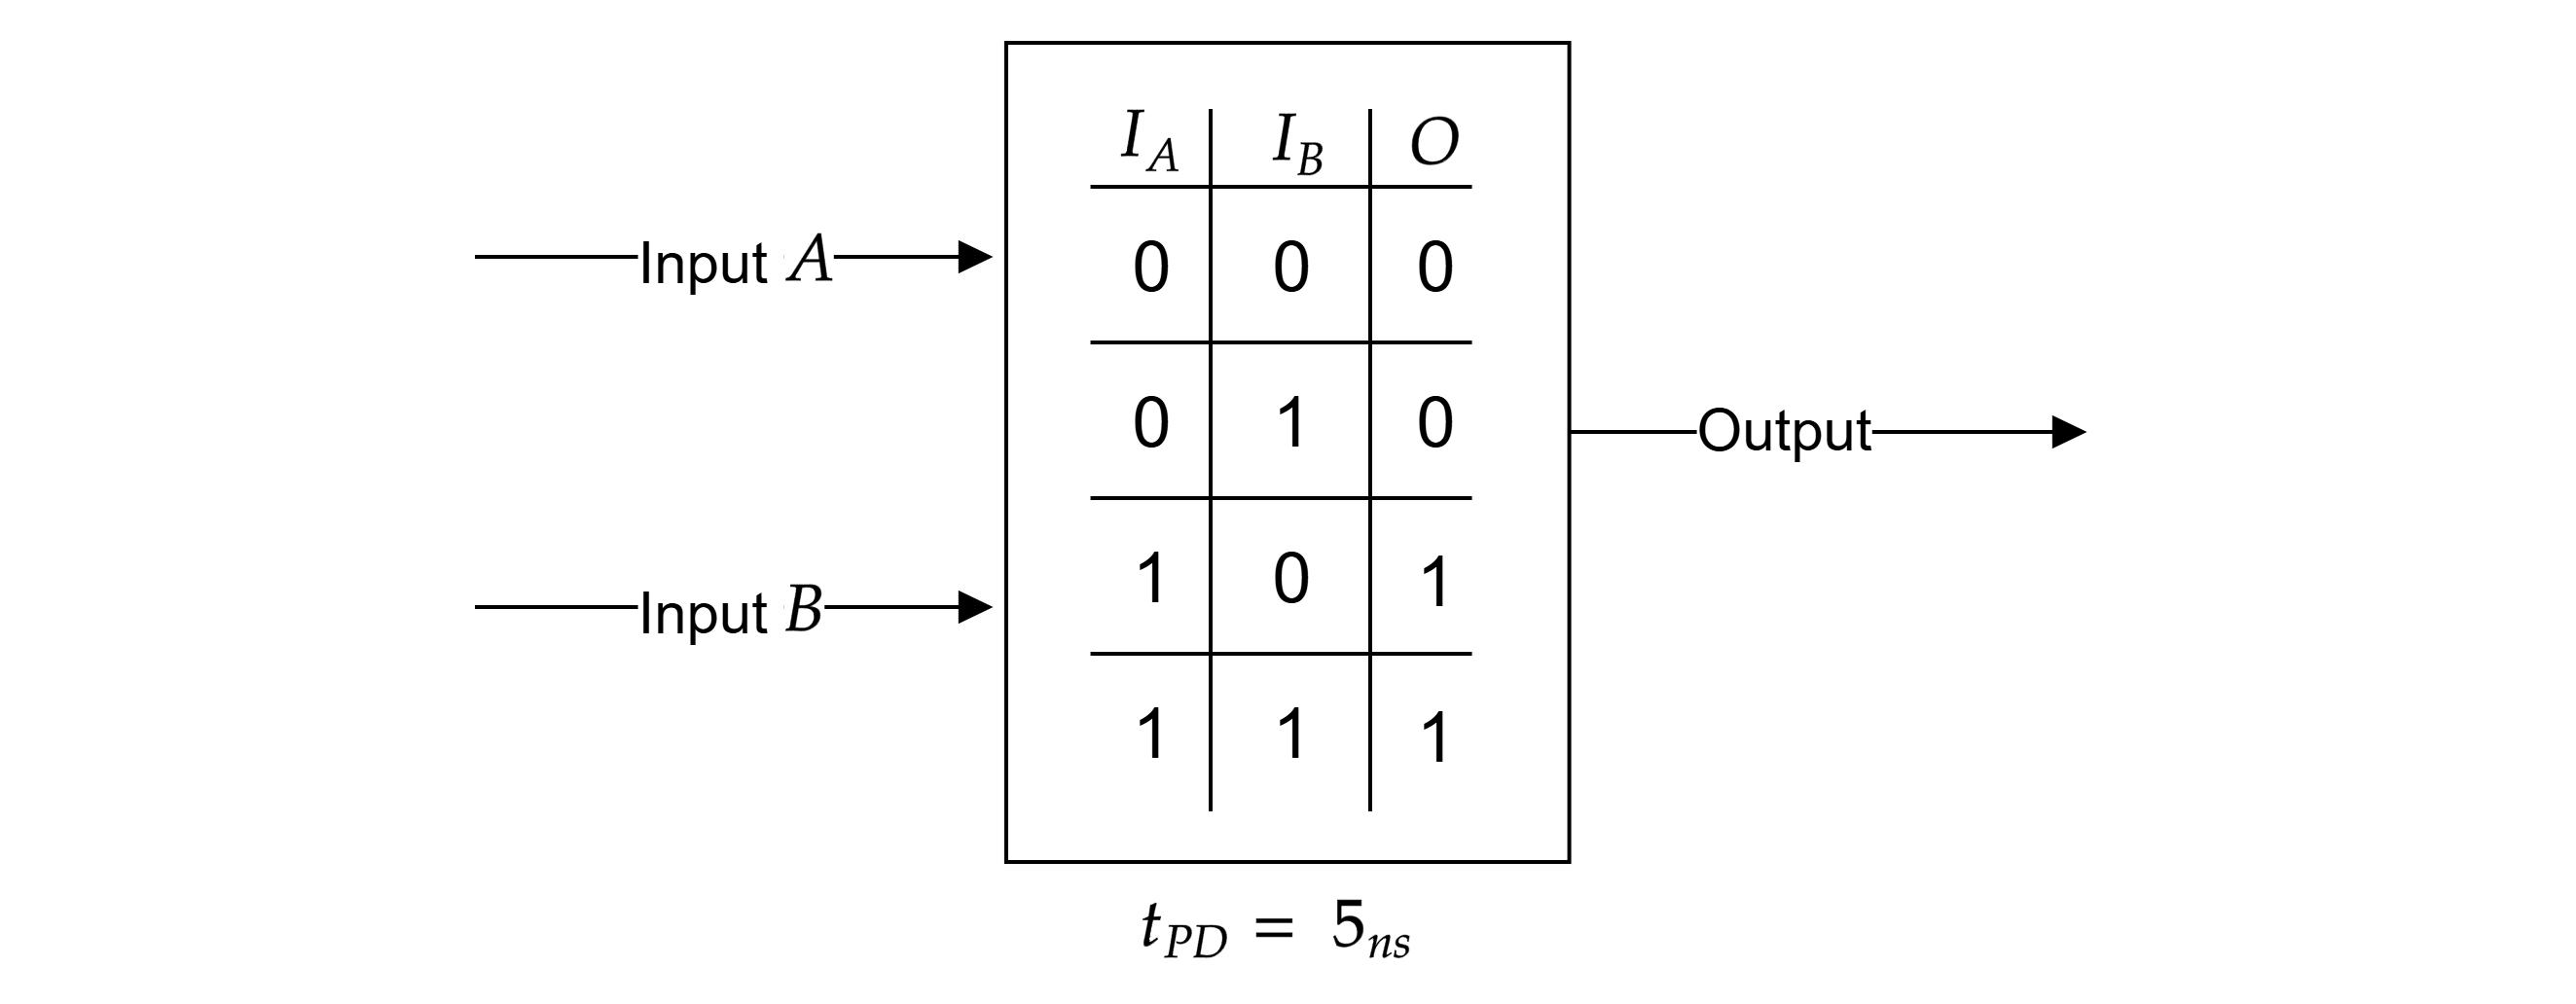
\includegraphics[width=.82\textwidth]{./Sections/circuits/combin.png}
        \caption{A combinational device with inputs $A$ and $B$, and a truth table detailing mappings towards the output.
        The $t_{PD}=5_{ns}$ (nanoseconds).}
        \label{fig:combinational_device}
    \end{figure}

    \newpage 

    \begin{Def}[Combinational Digital Systems]

        \label{def:combinational_digital_systems}

        \noindent
        A combinational device may also be made up of multiple other combinational devices. It must follow that:
        \begin{itemize}
            \item Each device is indeed a combinational device.
            \item Every input is connected to a single output.
            \item Each parent input will at most visit the same child input once (i.e., no cycles).
        \end{itemize}

        \noindent
        The $t_{PD}$ of the system is the sum of sub-devices $t_{PD}$'s along a path such that it is the 
        maximum such $t_{PD}$ path in the system.
    \end{Def}

    \vspace{-1em}

    \begin{figure}[ht!]

        \centering
        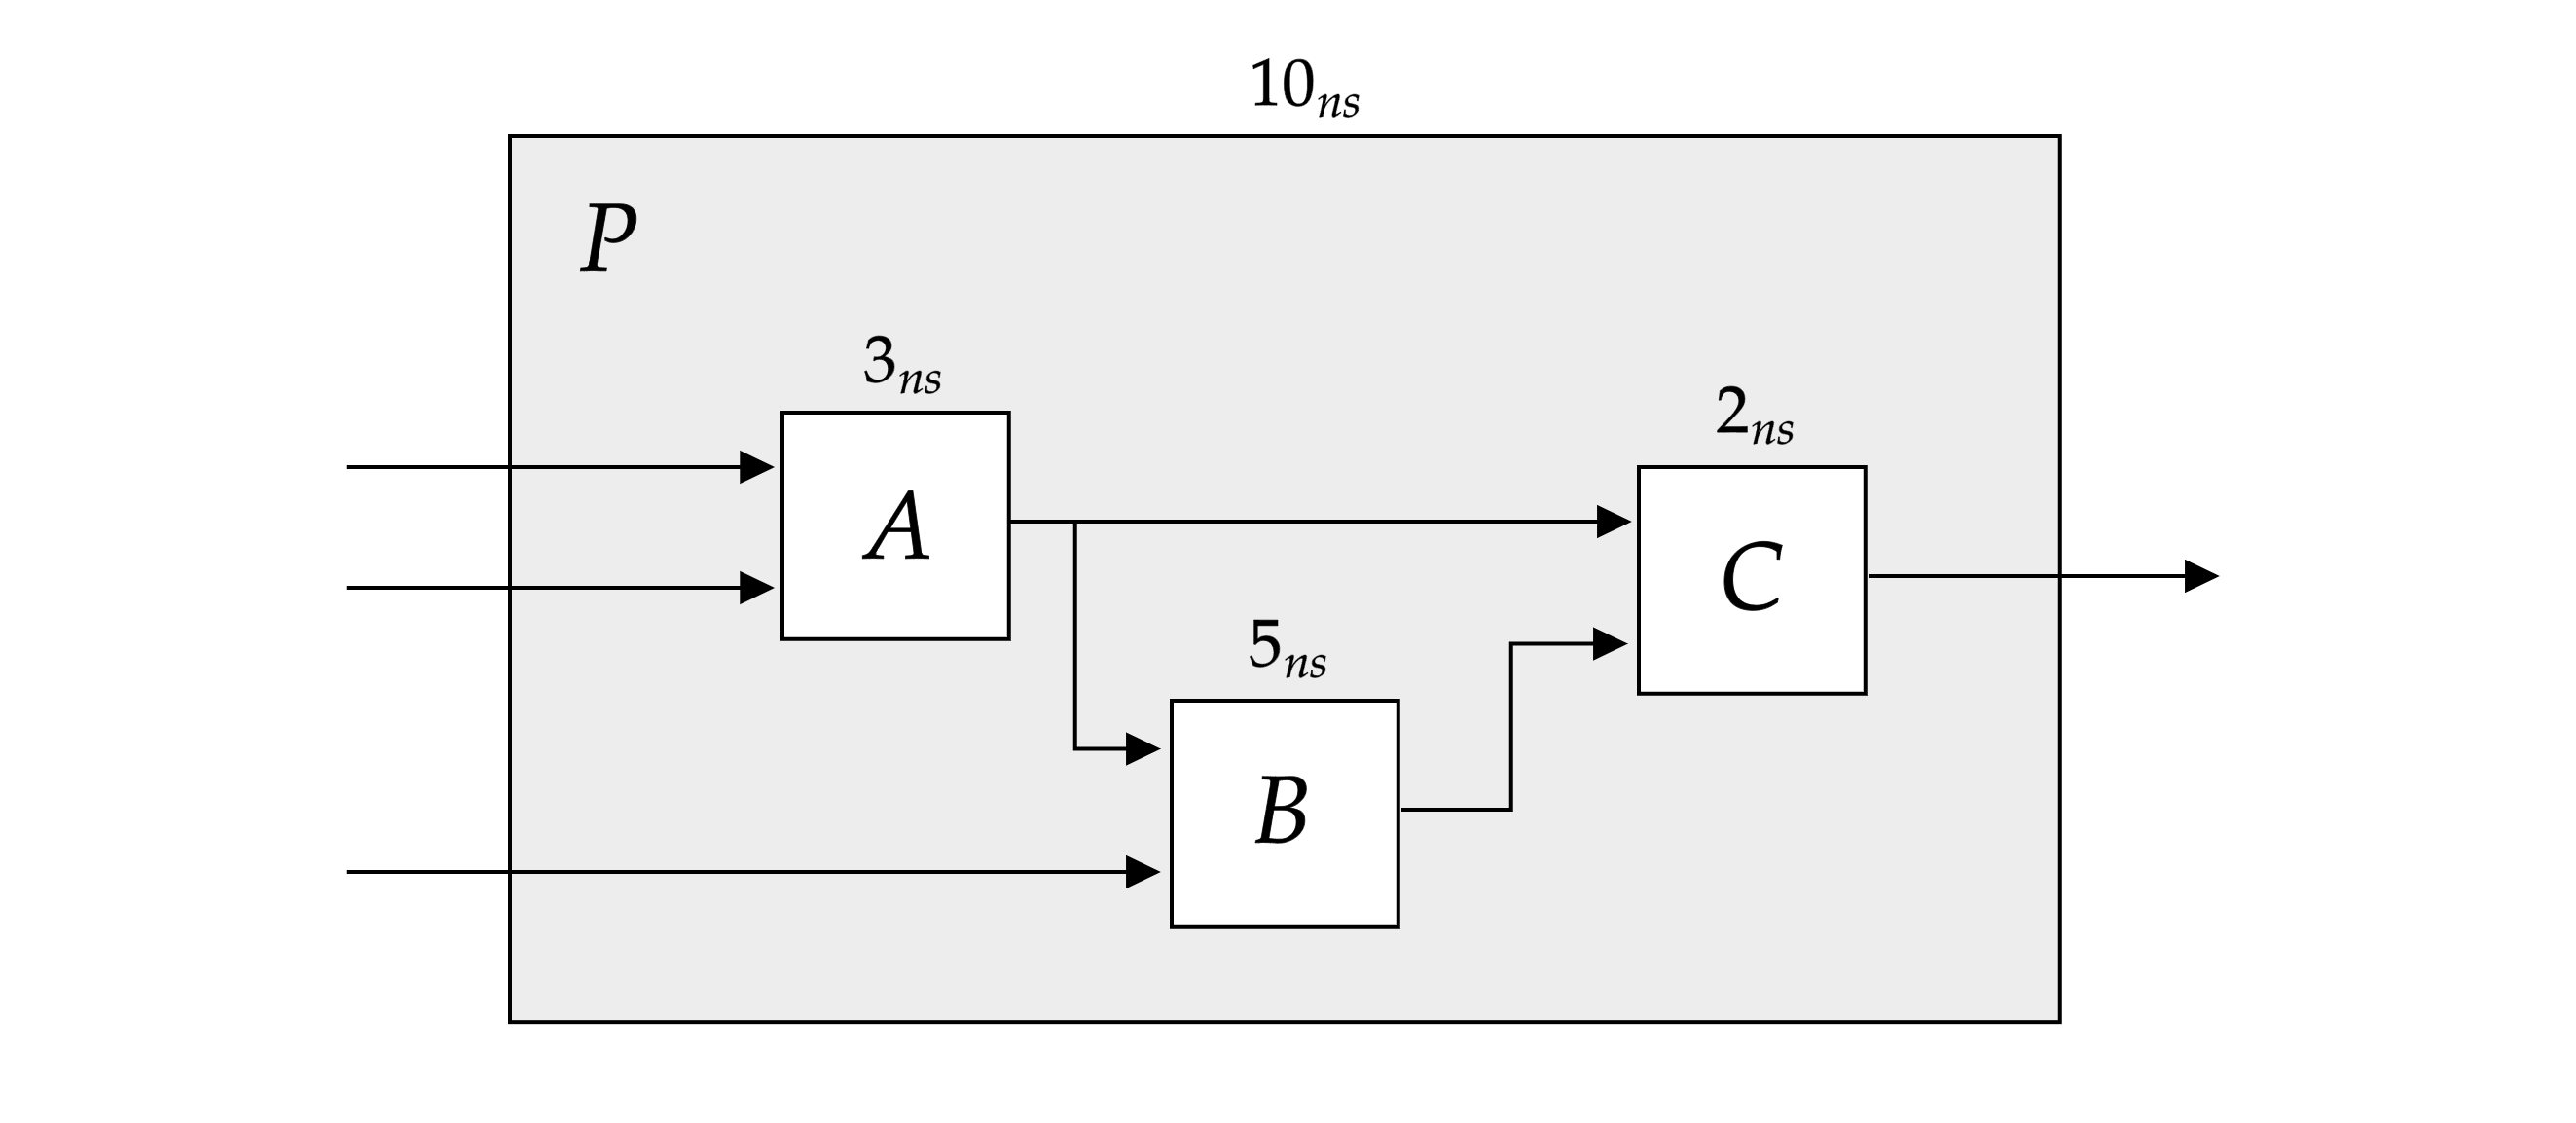
\includegraphics[width=.9\textwidth]{./Sections/circuits/combin_system.png}
        \caption{A combinational digital system, with a parent device $P$ and children devices $A,B$ and $C$.
        We abstract away the mappings focusing on the components and their connections. We see that there are no cycles and 
        all sub components are also combinational devices; Hence, the parent system is a combinational device. The 
        $t_{PD}$ of the system is $10_{ns}$, as the longest path takes $A\to B \to C = 3_{ns} + 5_{ns} + 2_{ns} = 10_{ns}$, the 
        effective bottleneck of the system.
        }
        \label{fig:combinational_digital_systems}
    \end{figure}

    \noindent
    Though this introduces a new problem:
    \begin{figure}[ht!]

        \centering
        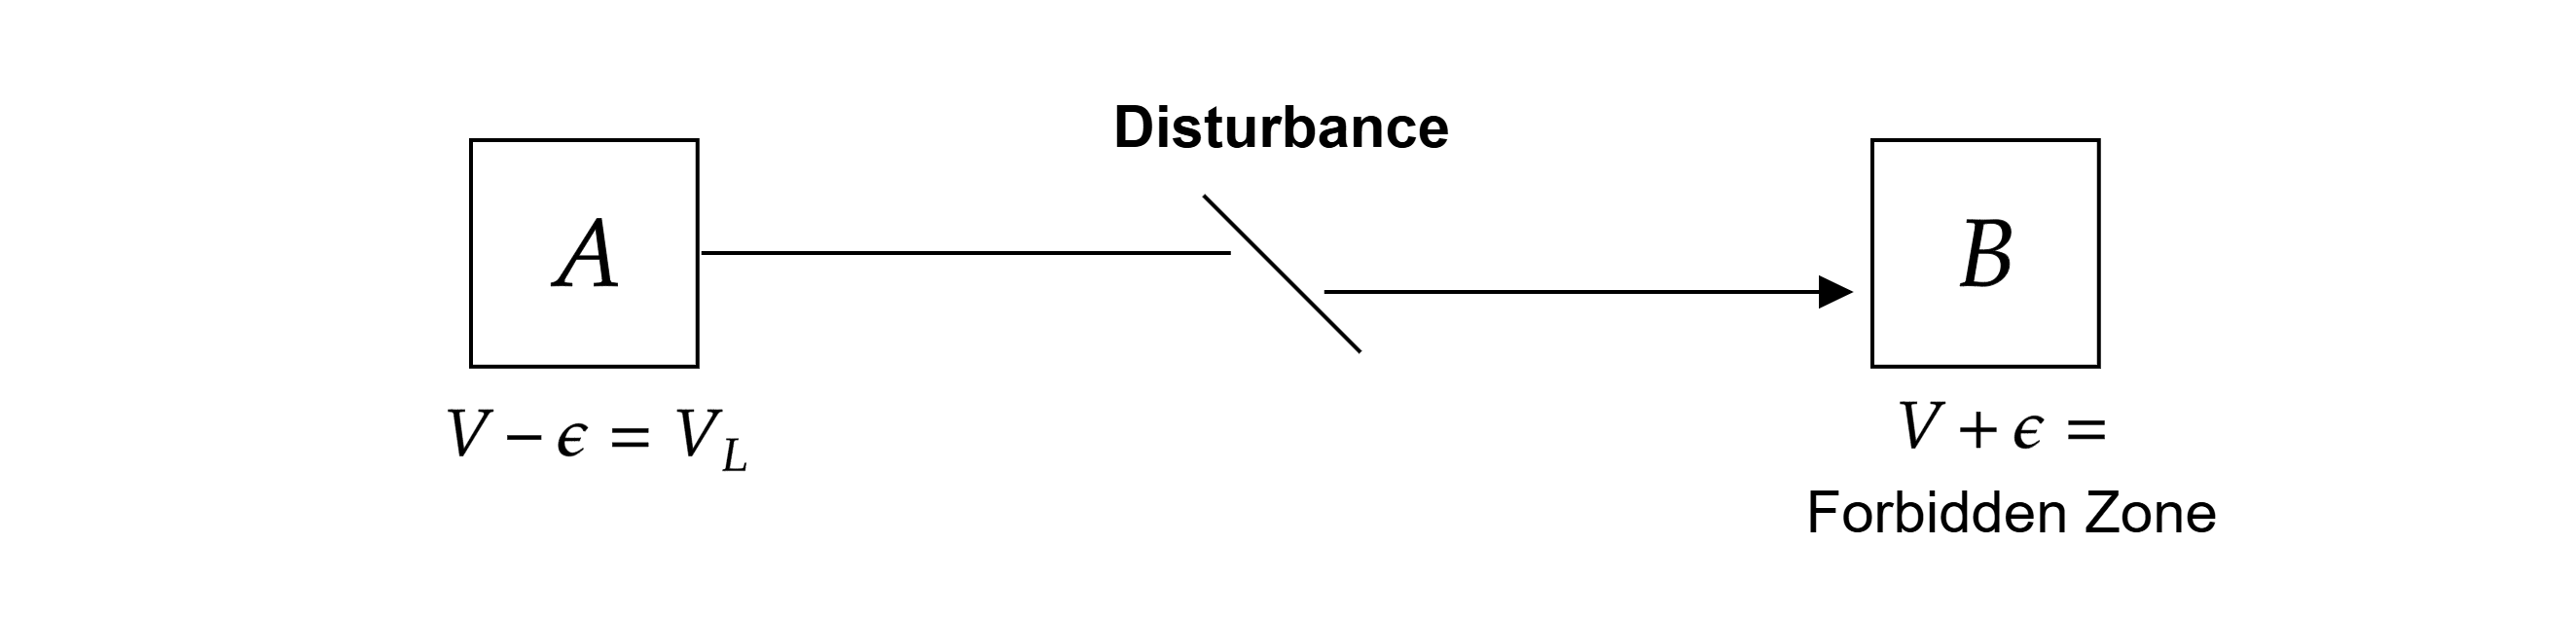
\includegraphics[width=.82\textwidth]{./Sections/circuits/combin_noise.png}
        \caption{Combinational devices $A$ and $B$ communicate; However, $A$'s output ($V$) is dangerously close 
        to $V_{L}$, over the wire there is a disturbance, causing the input of $B$ to enter the forbidden zone.}
        \label{fig:combinational_digital_systems_cycle}
    \end{figure}

    \newpage 

    \noindent
    We offer a simple fix to this problem, by loosening up the thresholds during certain phases:

    \begin{Def}[Noise Margins]

        \noindent
        To mitigate noise from outputs of a combinational device, we decrease the \emph{forbidden zone} (FZ) for the 
        receiving device. The overlap between the output's FZ and the input's FZ is called the \textbf{noise margin}.
        Concretely, we define the following:\\

        \noindent
        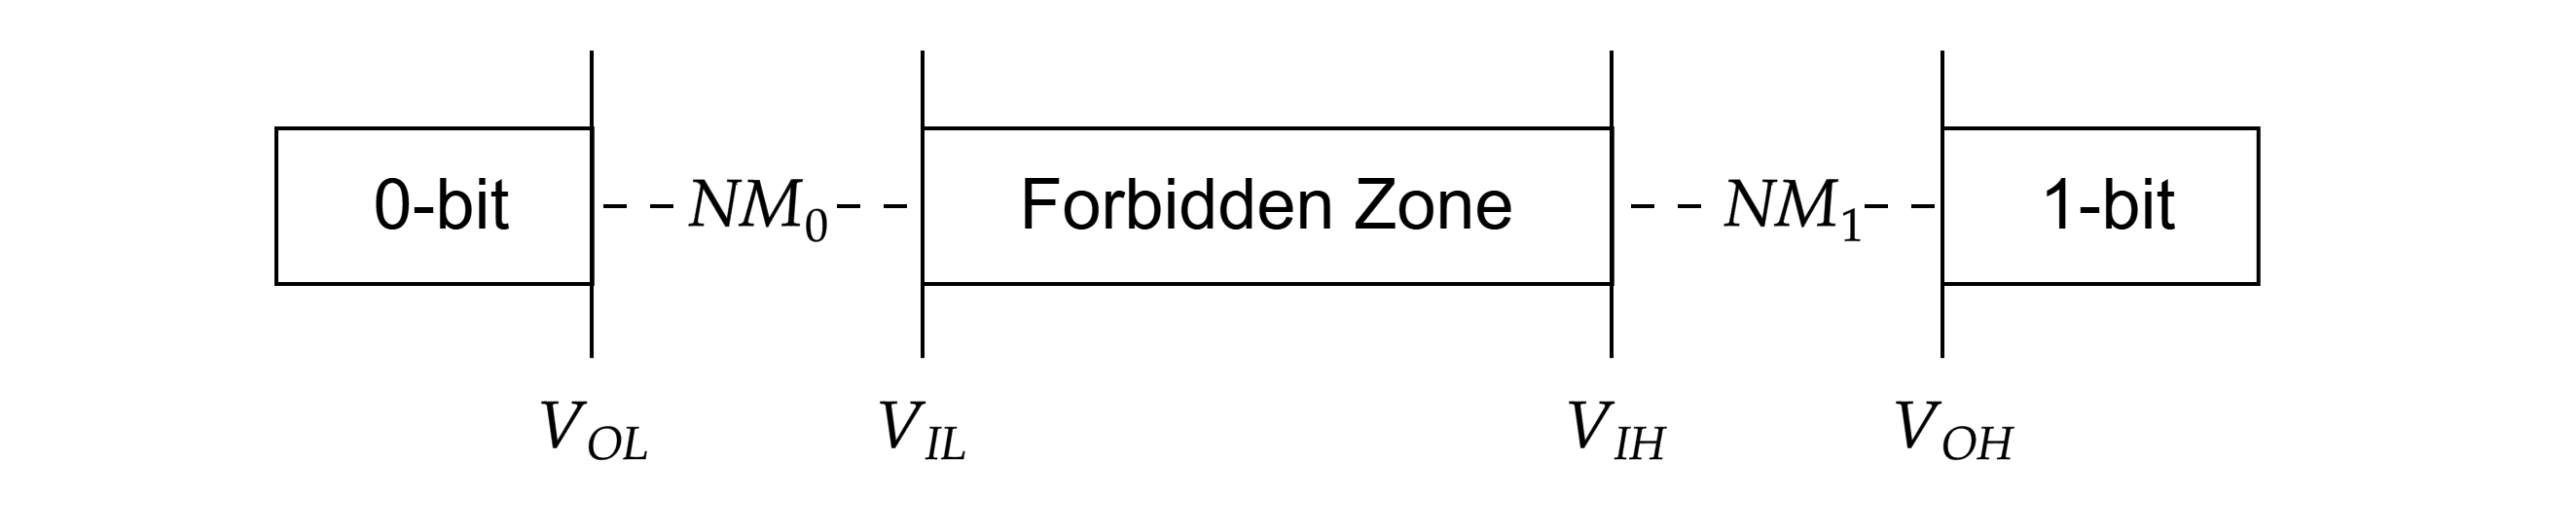
\includegraphics[width=\textwidth]{./Sections/circuits/noise_margin.png}

        \noindent
        Where, $V_{OL}$ and $V_{OH}$ are the output bounds, while $V_{IL}$ and $V_{IH}$ are the new input bounds.
        Then $\mathrm{NM}_0$ is the noise margin for the 0-bit, and $\mathrm{NM}_1$ is the noise margin for the 1-bit. The smallest 
        of the two is called the \textbf{noise immunity} of the device (i.e., the worst case that must be supported).
    \end{Def}


    \noindent
    Now when building our systems or combinational devices we must standardize how a particular device behaves on 
    inputs and outputs to account for the worst case noise.
    \begin{Def}[Voltage Transfer Characteristics (VTC)]

        \label{def:vtc}

        \noindent
        The \textbf{Voltage Transfer Characteristics} (VTC) is a graphical representation which shows how a device's inputs
        affect its outputs after stabilization. The horizontal axis measures the input voltage, while the vertical axis measures the output voltage.

        \begin{itemize}
            \item \textbf{Horizontal Axis ($V_{in}$):} Contains $V_{IL}$ and $V_{IH}$:
            \[V_{in} \leq V_{IL} \text{ (0-bit)} \quad \text{and} \quad V_{in} \geq V_{IH} \text{ (1-bit)}\]
            \noindent
            Otherwise, the input is in the forbidden zone.
            \item \textbf{Vertical Axis ($V_{out}$):} Contains $V_{OL}$ and $V_{OH}$:
            \[V_{OL} < \text{Invalid Outputs} < V_{OH} \quad \text{such that} \quad V_{in} < V_{OL}, V_{in} > V_{OH}\]
            \noindent
            I.e., if the input is already in the forbidden zone, the output is irrelevant.
        \end{itemize}

        \noindent
        It's given that the device must perform properly such that a $V_{in} > V_{IH}$ will always yield a $V_{out} > V_{OH}$, and a $V_{in} < V_{IL}$ will always yield a $V_{out} < V_{OL}$.
        Each device has its own VTC, plotting the input-output relationship. The resulting curve is the \textbf{VTC} of the device.
    \end{Def}

    \noindent
    \underline{Diagram next page.}

    \newpage

    \begin{figure}[ht!]

        \centering
        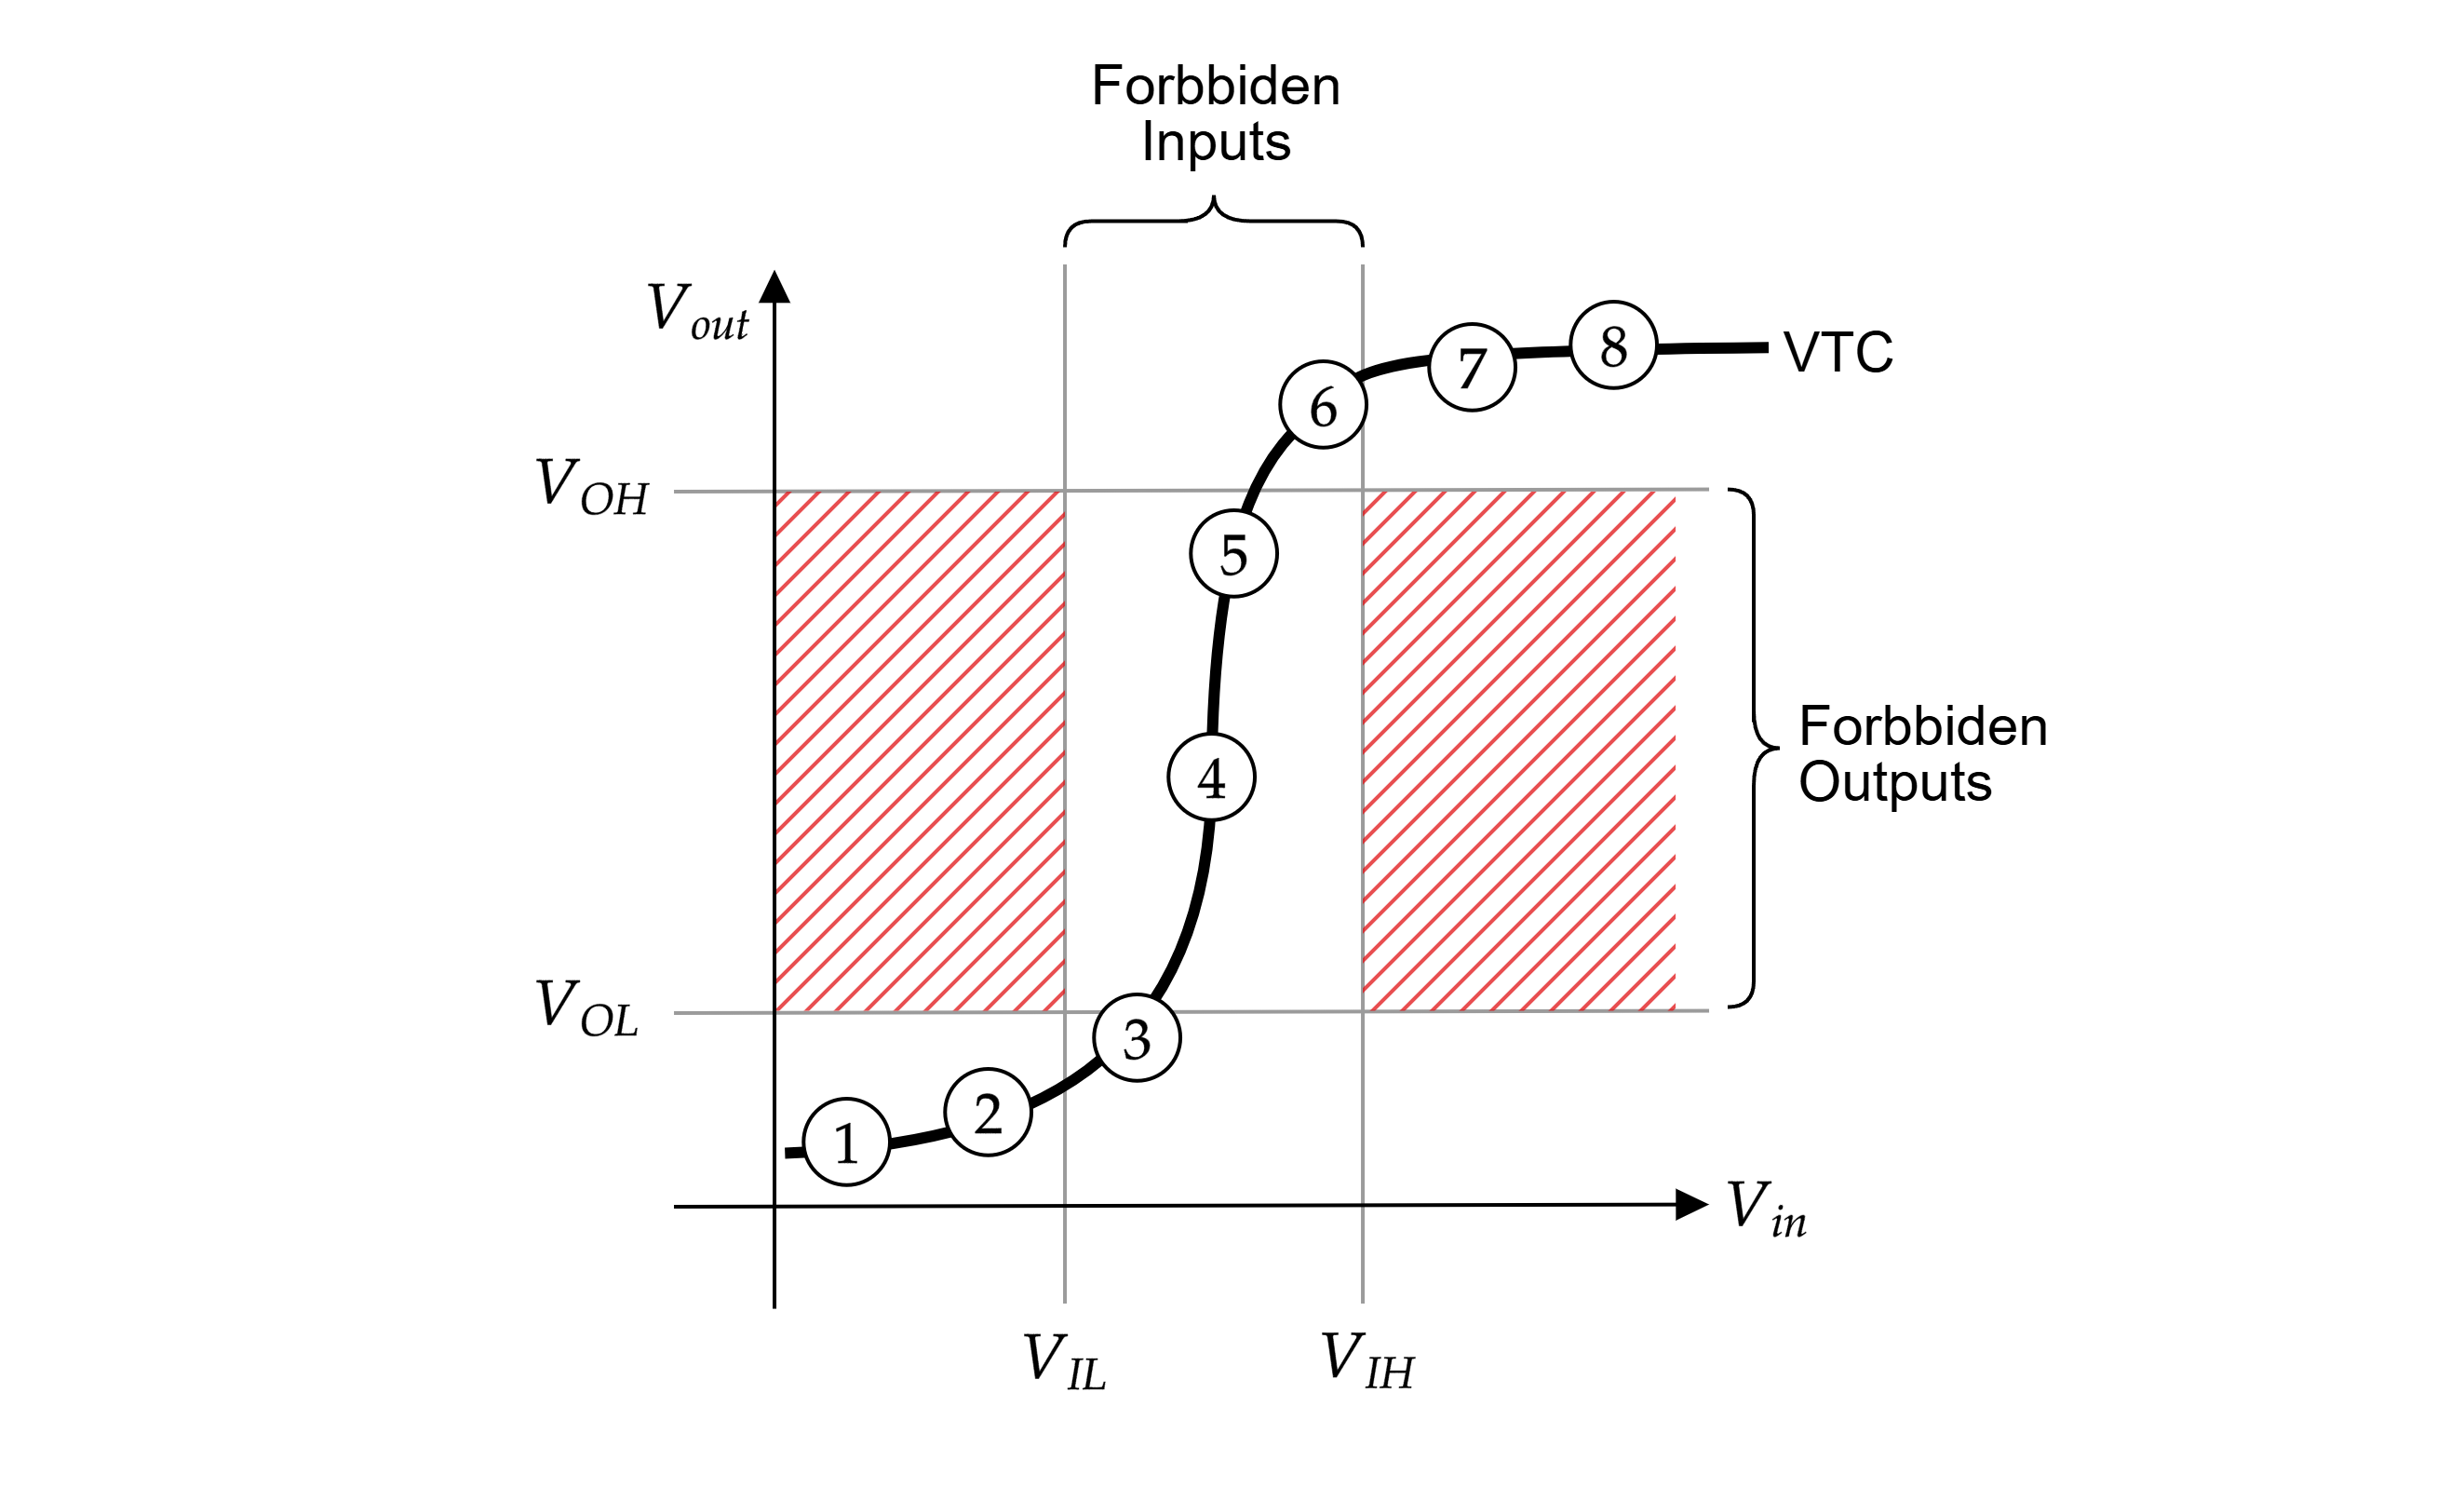
\includegraphics[width=\textwidth]{./Sections/circuits/vtc.png}
        \caption{A Voltage Transfer Characteristics (VTC) diagram, showing the input-output relationship of a device. 
        The horizontal axis represents the input voltage, while the vertical axis represents the output voltage. 
        The invalid output regions are shaded in red. The VTC is the bold line that crosses each point. \textbf{Note:} We don't care about the output when the input 
        is already in the forbidden zone, hence the output is undefined in that region. Moreover, the VTC is allowed flexibility
        to fluctuate in such regions.}
        \label{fig:vtc}
    \end{figure}
\newpage 

\subsection{Building Transistors: The Chemistry of Silicon}

\noindent
To even begin to manage currents and voltages, we will need a way to control the flow of electricity:

\begin{Def}[Transistor]

    \label{def:transistor}

  A \textbf{transistor} is a small electronic semiconductor device. A \textbf{semiconductor} (e.g., silicon) is a material with electrical 
    conductivity between that of a \textbf{conductor} (great electricity conductor) and an \textbf{insulator}
    (inhibits electric flow). Transistors fall into two broad families:

  \begin{itemize}
    \item \textbf{Bipolar Junction Transistor (BJT):} a current-controlled device with three terminals (pins),
    \begin{itemize}
        \item \textbf{Emitter (E):} current flows \emph{out}.
        \item \textbf{Base (B):} controls operation.
        \item \textbf{Collector (C):} current flows \emph{in}.
    \end{itemize}
    \item \textbf{Field-Effect Transistor (FET):} a voltage-controlled device with three terminals,
    \begin{itemize}
        \item \textbf{Source (S):} current flows \emph{in}.
        \item \textbf{Gate (G):} controls operation.
        \item \textbf{Drain (D):} current flows \emph{out}.
    \end{itemize}
  \end{itemize}

  \noindent
  Low-power transistors are molded in an epoxy (resin) package. Higher-power transistors often use a metal tab or ``can'' that you bolt to a \textbf{heat sink} (a metal object that dissipates heat).

  Pin order and package style vary by model; check the \textbf{part number} and manufacturer's \textbf{datasheet} for exact details \cite{what_is_transistor2022, engineermindset2024mosfet}.
\end{Def}

\begin{figure}[ht!]
  \centering
  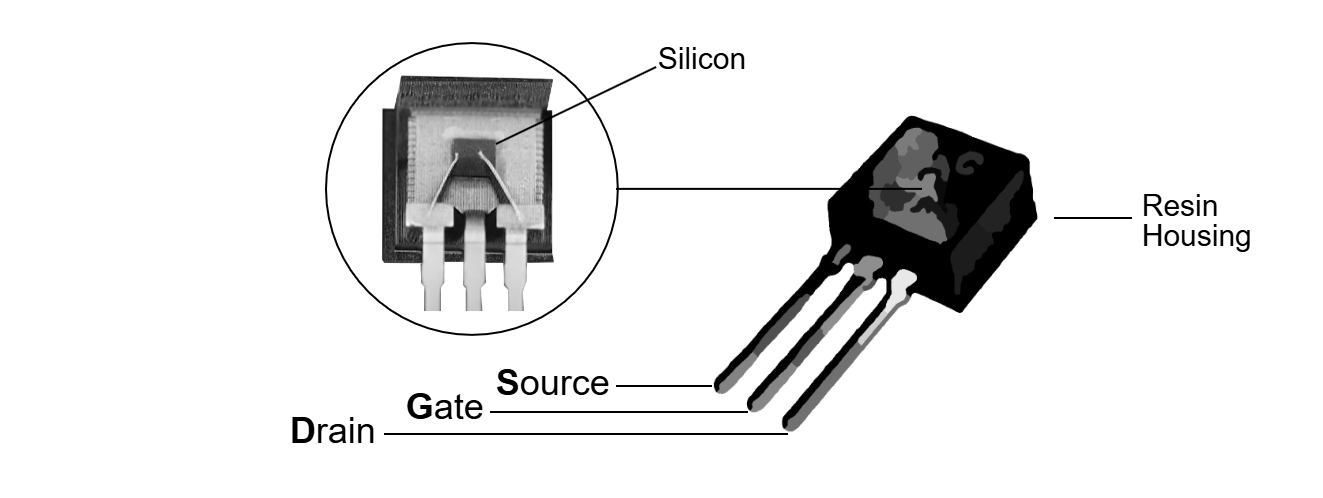
\includegraphics[width=\textwidth]{Sections/circuits/transistor.png}
  \caption{Cross-section of a discrete transistor: a silicon die (center) is bonded to three metal leads, all
    encased in an epoxy package.  A metal tab (not shown) may be added for heatsinking.}
  \label{fig:transistor}
\end{figure}

\newpage 



\begin{theo}[FETs over BJTs]

  \label{theo:why_mosfets_preferred}

  A BJT needs continuous base current, which wastes energy. A MOSFET only requires its gate to be charged or discharged (i.e., voltage applied or removed), which is more efficient.
\end{theo}

\noindent 
Now we briefly step into chemistry for completeness sake to understand differing silicon charges:
\begin{Def}[Anotomy of an Atom]

    \label{def:atom}

    An \textbf{atom} is the smallest unit of matter that retains the properties of an element. It consists of three main subatomic particles:
    \begin{itemize}
        \item \textbf{Protons:} Positively charged particles found in the nucleus.
        \item \textbf{Neutrons:} Neutral particles also found in the nucleus (same size as protons).
        \item \textbf{Electrons:} About the same charge as proton, but negative, and about 1800x smaller and lighter than a proton.
    \end{itemize}

    \noindent
    Protons and neutrons are tightly packed together in a space called the \textbf{nucleus}, gaining the name \textbf{nucleons};
    Electrons orbit the nucleus at discrete distances called \textbf{shells} or \textbf{energy levels}. 
    \underline{The number of protons in the nucleus defines the element (i.e., specifications).} E.g., 79 protons will 
    always be gold.

    Opposite charges attract, causing an \textbf{orbital space}, in which subatomic particles never collide (i.e., alike orbiting planets). Neutrons act as a buffer between protons (e.g., Silver is 
    stable with 60 or 62 neutrons, but unstable with 61). Atoms with different number of neutrons are called \textbf{isotopes}, latin for ``same place''.
    Electrons may jump between shells and atoms. If there is a greater number of electrons to protons, the atom is \textbf{negatively charged} (anions), otherwise it is \textbf{positively charged} (cations)
    \cite{crashcourse2013nucleus}.
\end{Def}

\begin{Def}[Periodic Table]

    \label{def:periodic_table}

    The \textbf{Periodic Table of Elements} organizes all known elements by the number of protons in their nuclei. This is called an \textbf{atomic number} (e.g., 
    gold's atomic number is 79). Elements are abbreviated from their latin translations (e.g., gold is \textbf{aurum}, AU, which means ``shining dawn'').
    There are 118 elements, with 80 being stable and the rest being unstable isotopes. Anything past 82 protons (lead) is 
    unstable, undergoing radioactive decay.
\end{Def}

\begin{Tip} The periodic table is complete, hence movies that claim ``we discovered a new element!'' truly deserve science-fiction as their defining genre.
\end{Tip}
\newpage 
\noindent
We'll stop with the chemistry dive after these next two critical definitions

\begin{Def}[Shell Capacities \& Valence Electrons]

    \label{def:valence_electrons}

    The first shell of any atom can hold up to 2 electrons, and the second 8. From 1-20 periodic elements, the third and fourth 
    shells can hold 8 and 2 respectively. A \emph{full} shell is considered \textbf{stable}, otherwise it is \textbf{unstable}.
    This arrangement of electrons within the shells is called the \textbf{electron configuration} (EC) of the atom.
    An EC is written as a n-tuple, starting with the inner-most shell (e.g., 2, 8, 8, 2 for calcium).

    
    The outer most shell is called the \textbf{valence shell}. An atom's \textbf{valency} (the number of electrons in the valence shell) determines whether a chemical reaction will occur.
     If an atom is stable (i.e., full valence shell), it will not react with other atoms.
    Unstable atoms \emph{strive} to become stable by either gaining, losing, or sharing electrons with other atoms \cite{infinitylearn2018concept}.
\end{Def}

\begin{Def}[Chemical Bonds -- Molecules \& Compounds]

    \label{def:chemical_bonds}

    The act of atoms joining together (e.g., sharing electrons, which is called a \textbf{covalent bond}), forms a \textbf{molecule}. 
    Concretely, a molecule is a merger of two or more elements. We use subscripts to denote the number of atoms in a molecule (e.g., H$_2$O is water, with two hydrogen atoms and one oxygen atom).
    \textbf{Compounds} are a subset class of molecules that consists only of two more more \textbf{different} elements (e.g., H$_2$O is a compound, but O$_2$ is not, as it only has one element, oxygen)  \cite{breslyn2013molecule}.
\end{Def}
\noindent
Now to what we've been waiting for:
\begin{Def}[Doping -- N-type \& P-type Silicon]

    \label{def:doping}

    Silicon has 14 atoms, with an EC of (2, 8, 4); Hence silicon is unstable. If we view silicon (Si) as a 3D lattice (a string of Si atoms in 3D grid),
    each Si atom will share its four valence electrons with it neighbors to become stable (covalent bonding). This creates a \textbf{silicon crystal}.\\

    \noindent
    Adding another element to the silicon lattice is called \textbf{doping}. We 
    are interested in two types of doping \cite{engineermindset2024mosfet}:
    \begin{itemize}
        \item \textbf{N-type:} When adding an element like phosphorus (P), EC of (2, 8, 5), is added to the silicon lattice, one electron goes unused after the covalent bonding. This free electron creates a \textbf{negative charge carrier} (hence N-type).
        \item \textbf{P-type:} Conversely, adding boron (B), EC of (2, 8, 3), creates a \textbf{positive charge carrier} (hence P-type). This is because boron won't have 
        enough to share with its neighbors, causing \textbf{holes} (absence of electrons), overall lowering the density of electrons.
    \end{itemize}
\end{Def}

\newpage 

\noindent 
Let's visualize what we've learned so far:

\begin{figure}[ht!]

  \centering
  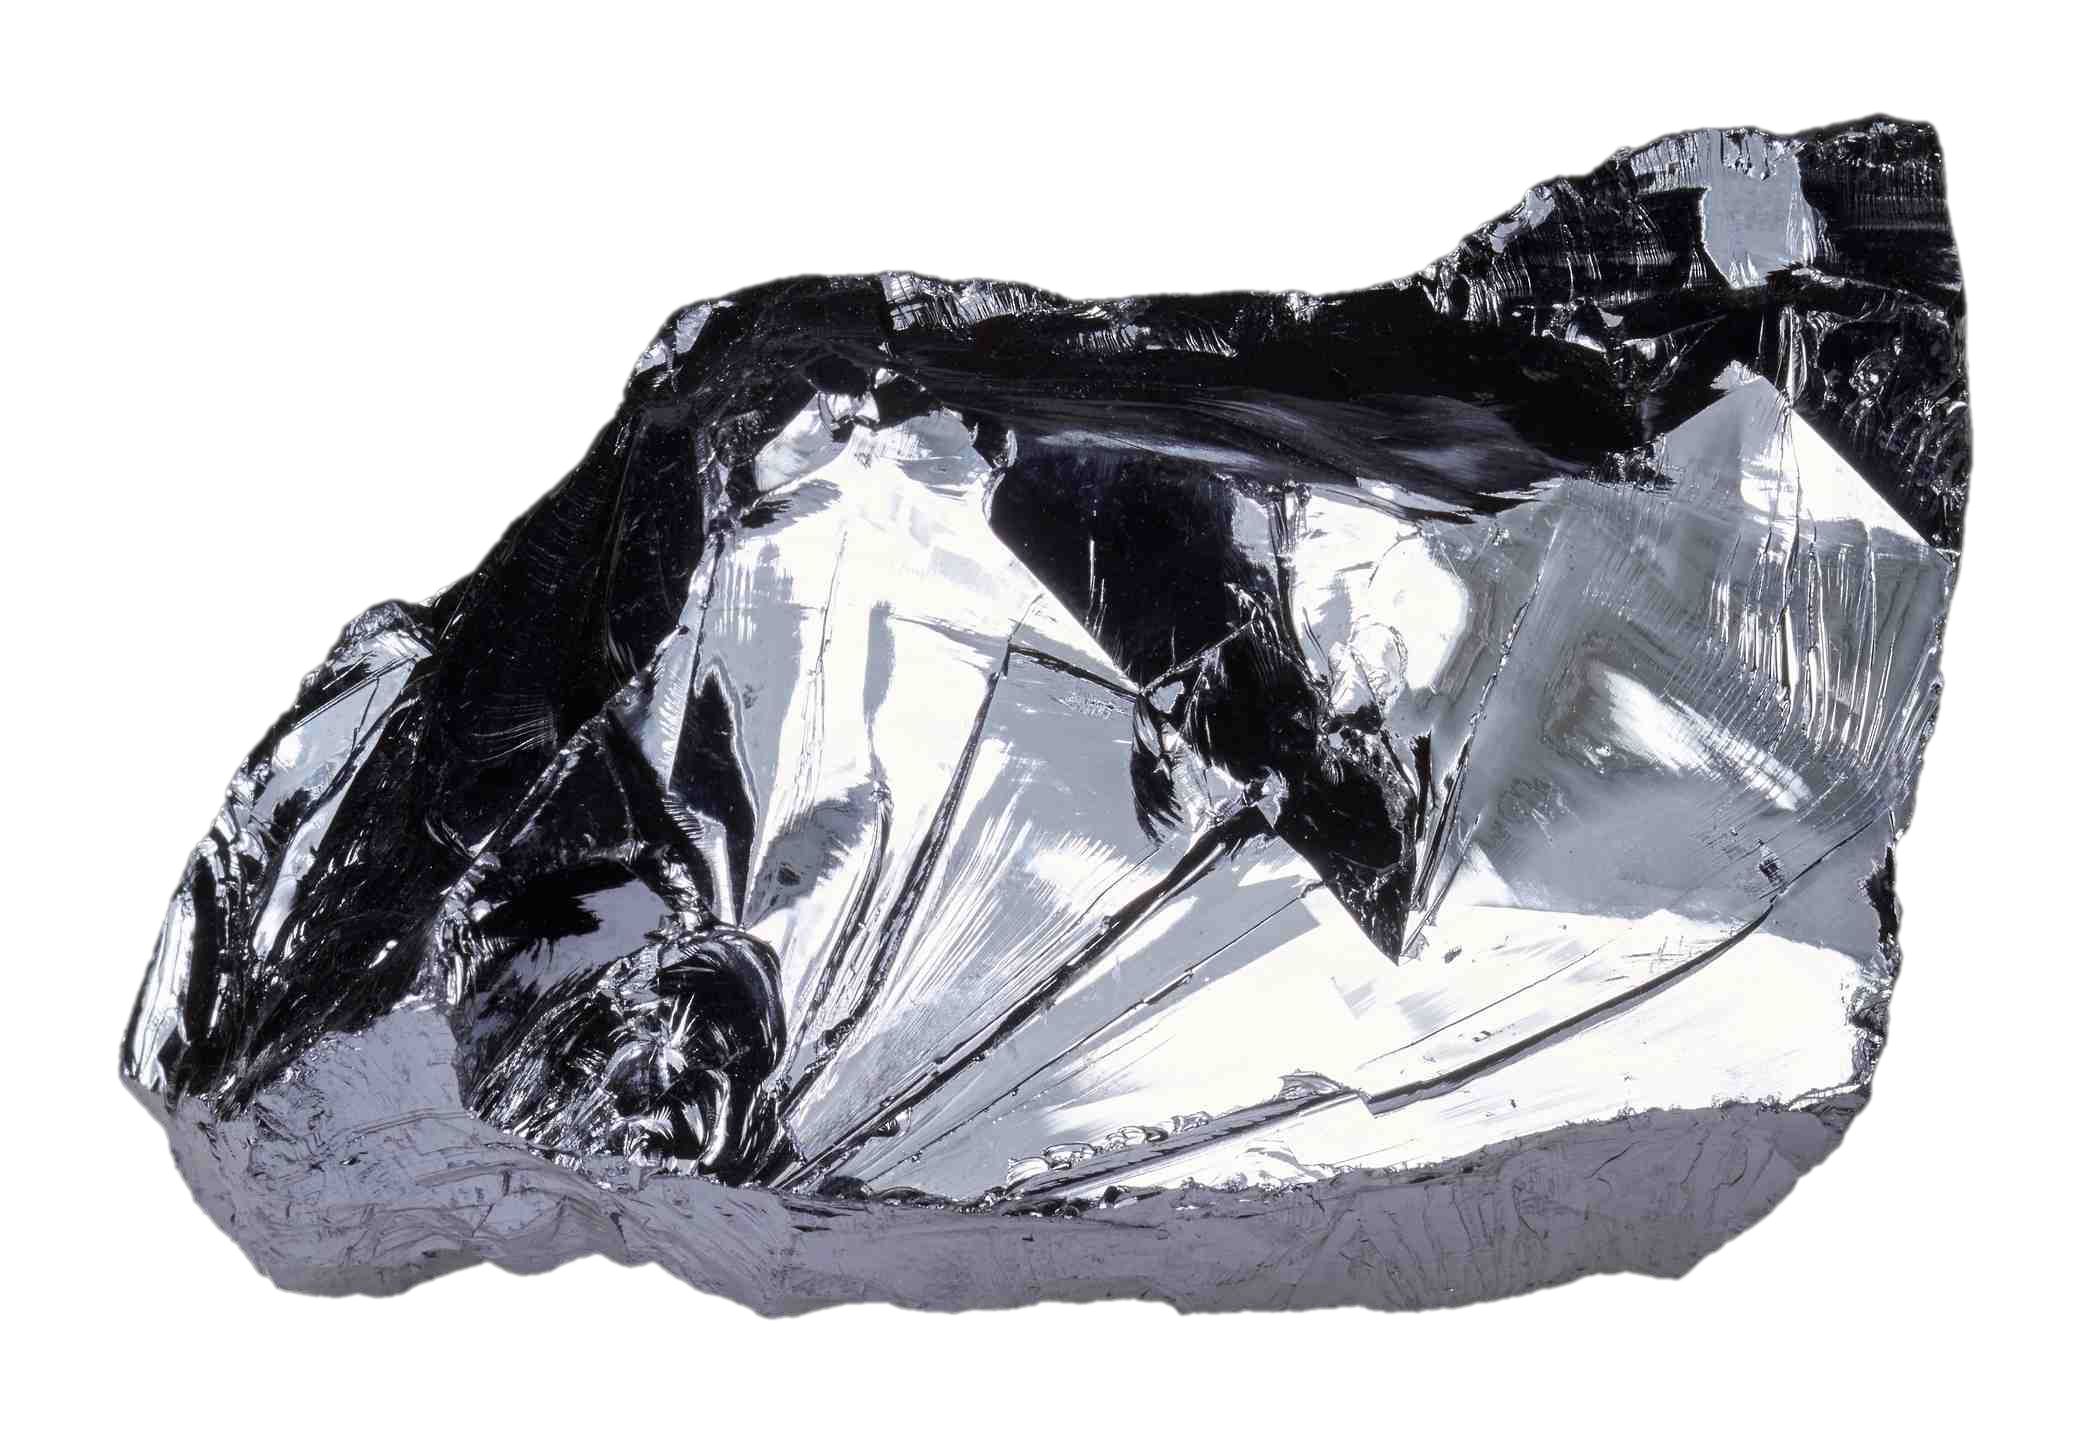
\includegraphics[width=.6\textwidth]{Sections/circuits/sicryst.jpg}
  \caption{An image of a silicon crystal \cite{gettyimages700832601}.}
  \label{fig:atom}
\end{figure}

\vspace{2em}
\begin{figure}[ht!]

  \centering
  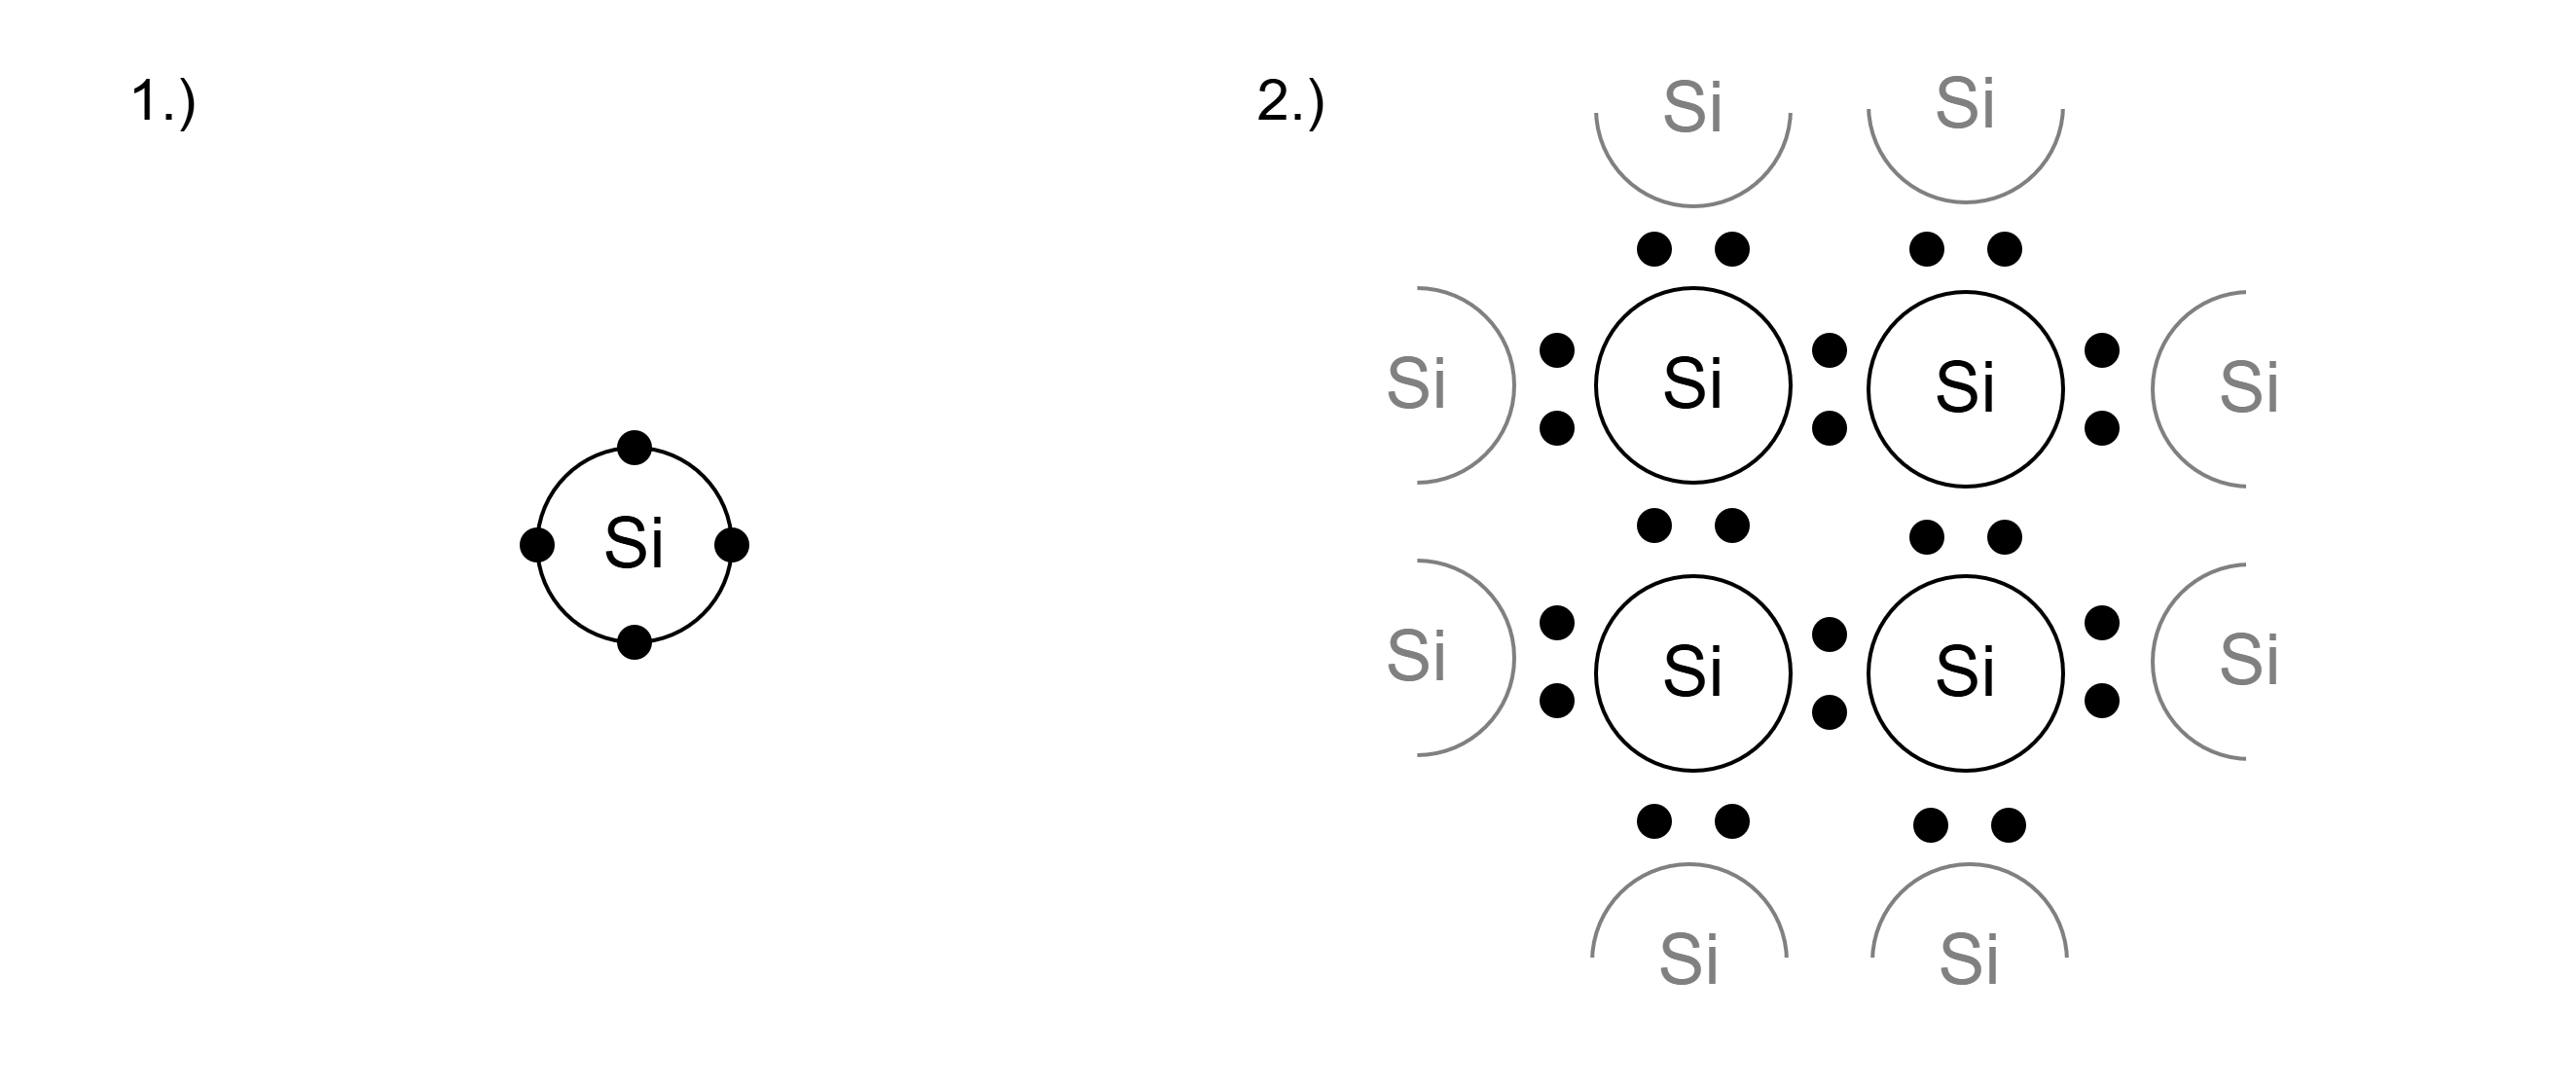
\includegraphics[width=\textwidth]{Sections/circuits/doping.png}
  \caption{(1) Shows a single silicon atom (Si) and its valence electrons (4 black dots).
  (2) Shows a flattened silicon lattice where neighboring Si atoms share their electrons to become stable.
  This creates an electron configuration of (2, 8, 8) for surrounded Si atoms.}
  \label{fig:doping}
\end{figure}
   
\newpage 

\noindent
\begin{figure}[ht!] 
  \centering
  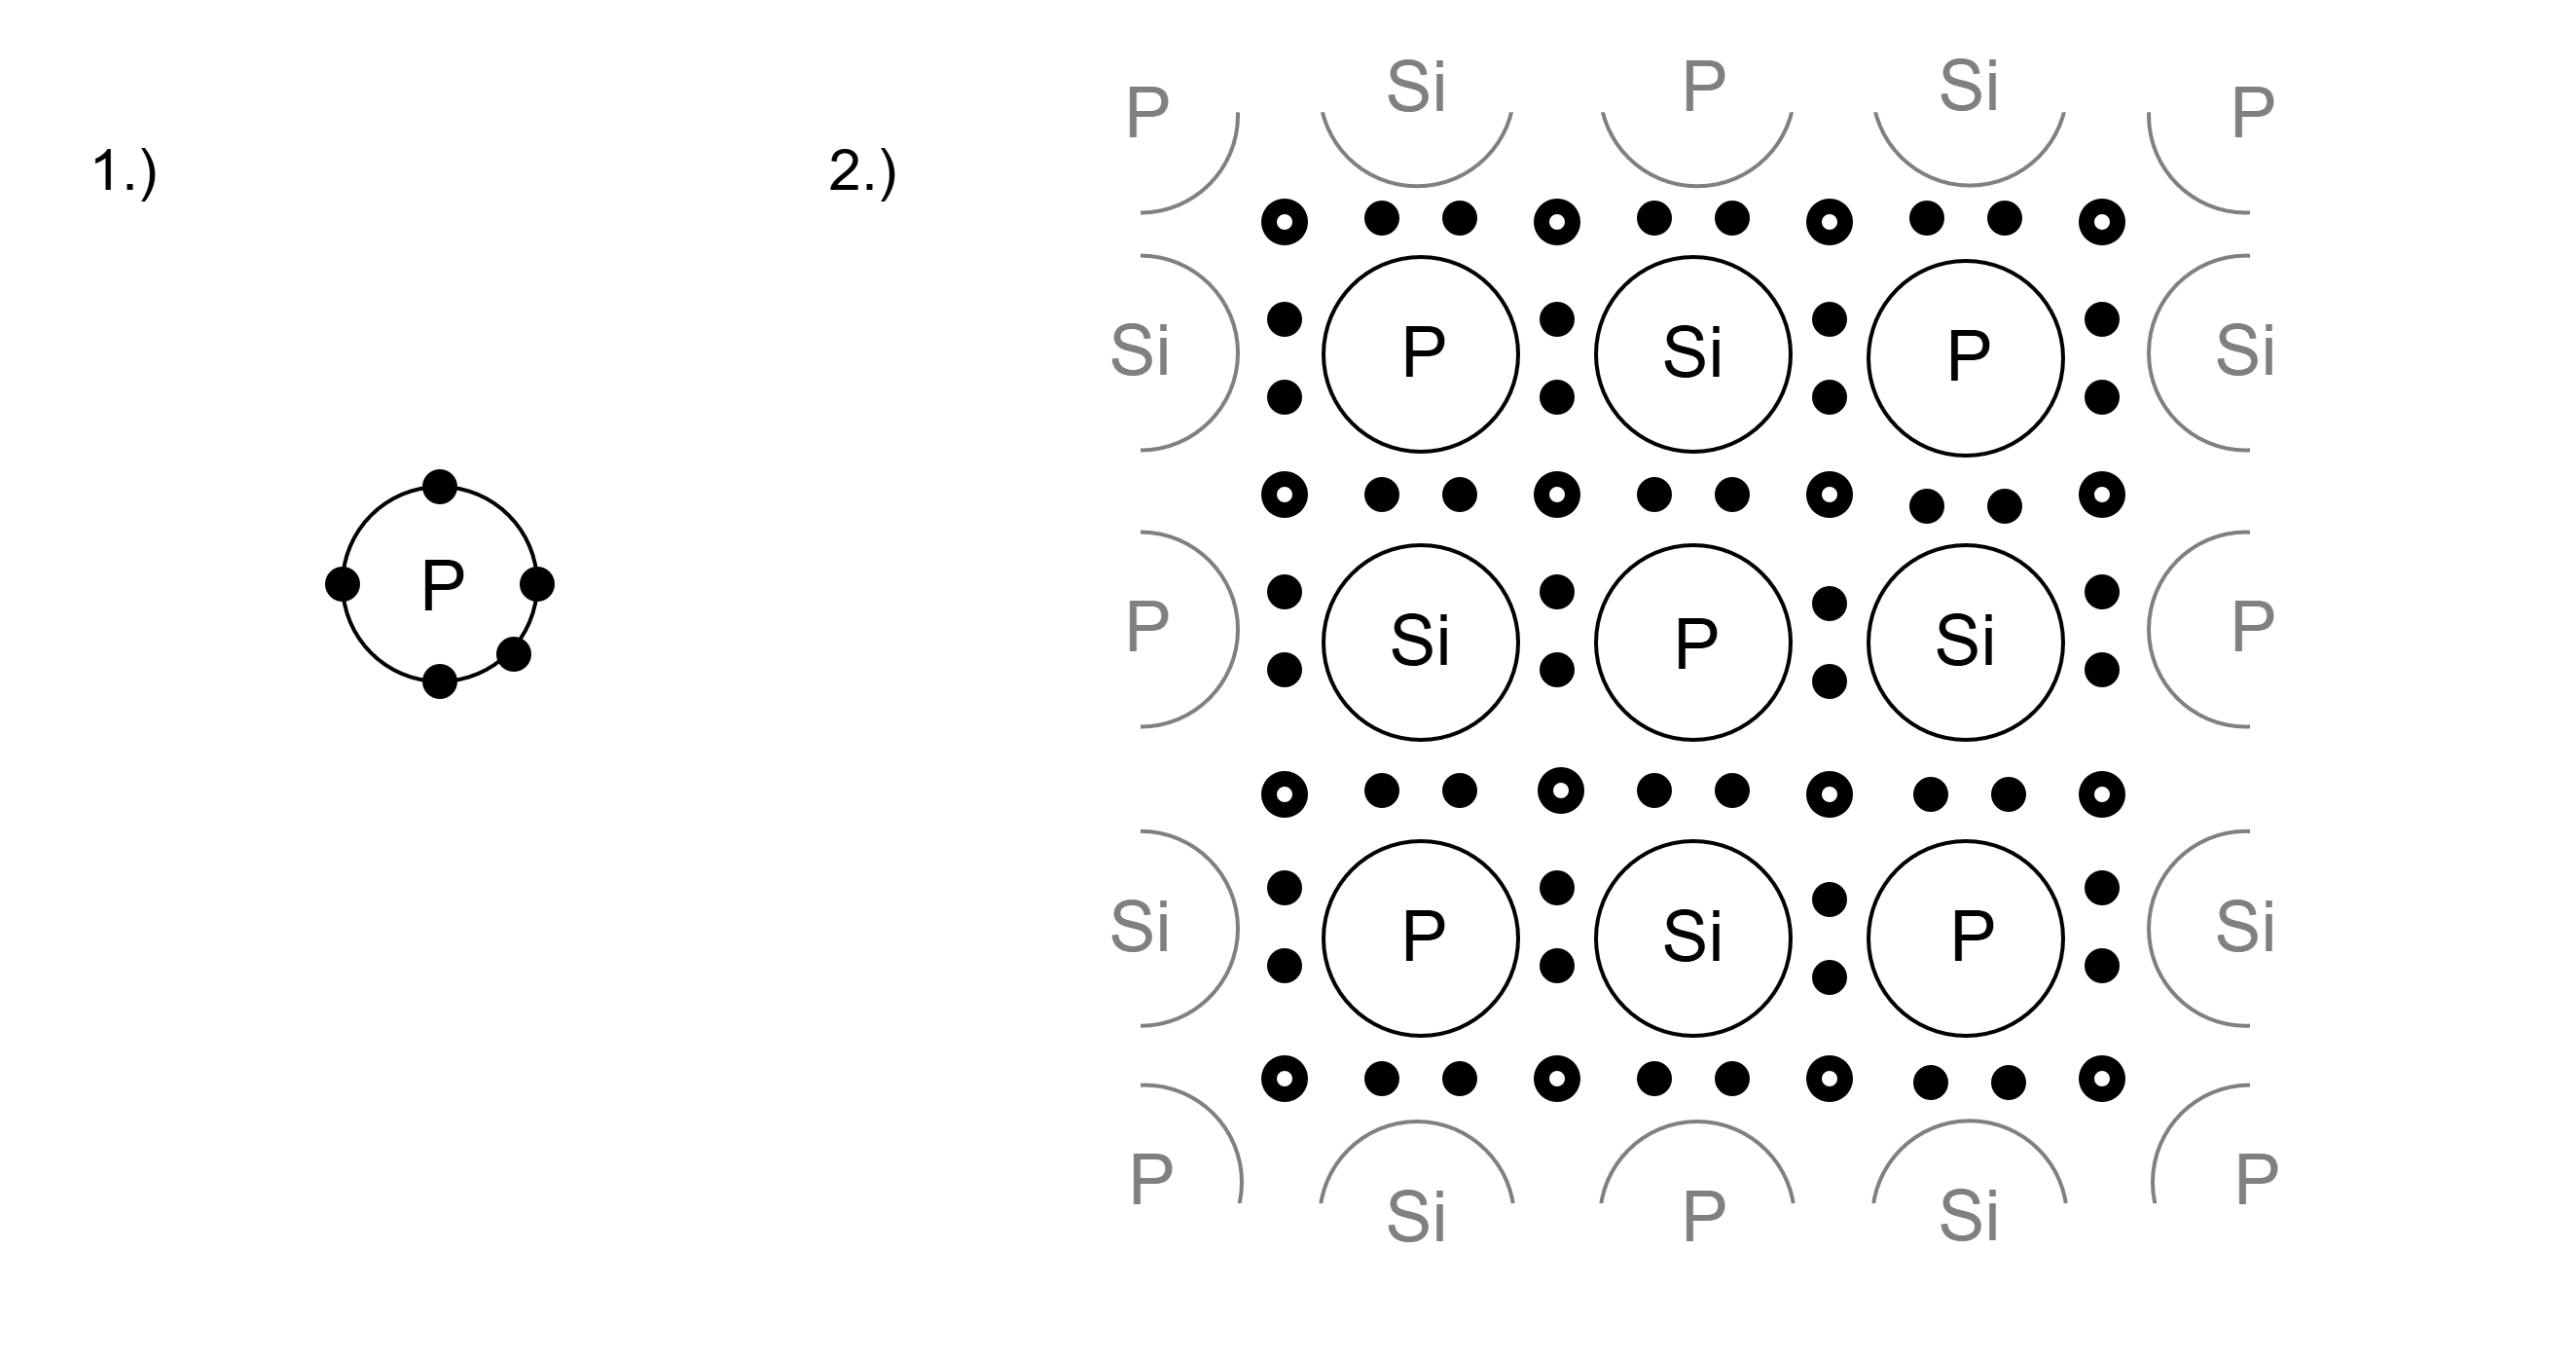
\includegraphics[width=\textwidth]{Sections/circuits/n-type.png}
  \caption{(1) Shows a single phosphorus atom (P) and its valence electrons (5 black dots).
  (2) A silicon lattice where phosphorus is doped, creating free electrons (thick dots with holes). }
  \label{fig:doping2}
\end{figure}

\vspace{-1em}
\begin{figure}[ht!]
  \centering
  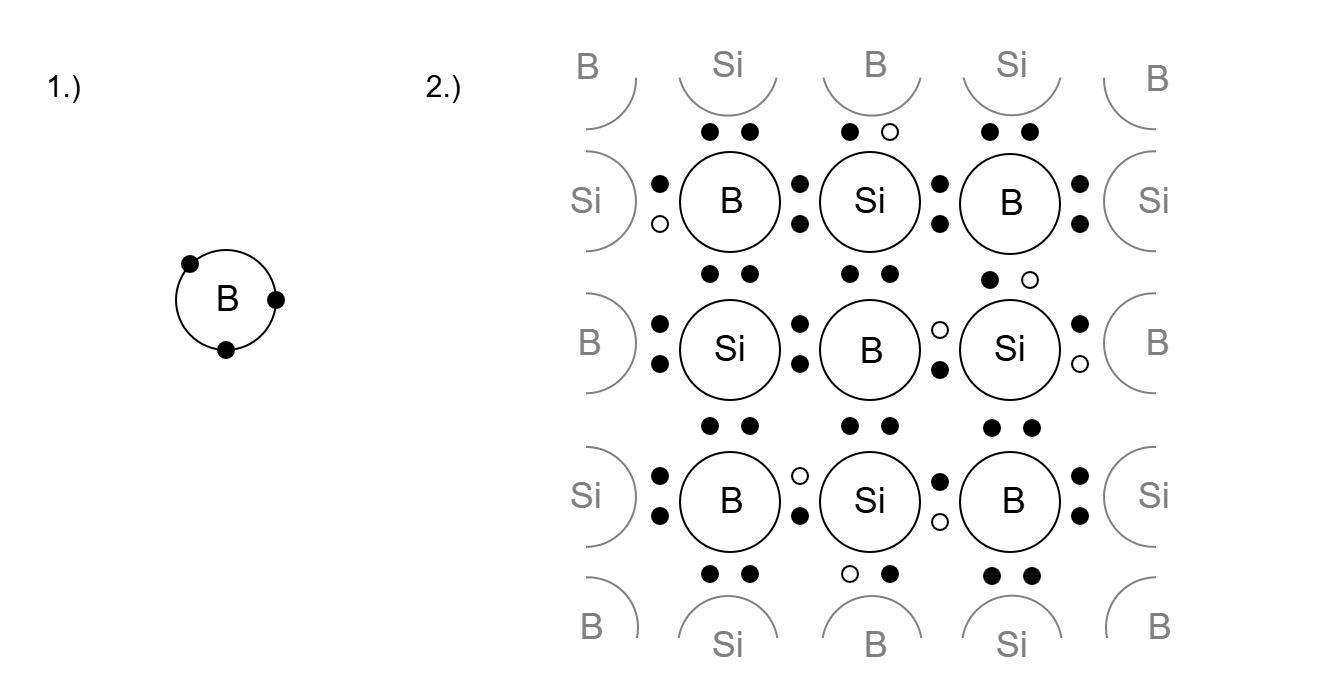
\includegraphics[width=\textwidth]{Sections/circuits/p-type.png}
  \caption{(1) Shows a single boron atom (B) and its valence electrons (3 black dots).
  (2) Shows a flattened silicon lattice where boron is doped, creating holes (halo dots). }
  \label{fig:doping3}
\end{figure}

\newpage 

\begin{Def}[N-type \& P-type Junctions]

    \label{def:n_p_junctions}

   When a N-type and P-type material are placed next to each other 
   creates a \textbf{PN-junction}. At this junction, we get a \textbf{depletion region},
   where N-type electrons and P-type holes cross; This leaves a 
   slightly positive region on the N-type side and a slightly negative region on the P-type side.
   This manifests an electric field, creating a barrier, preventing further flow across the junction \cite{engineermindset2024mosfet}.
\end{Def}

\vspace{-1.5em}
\noindent
\begin{figure}[ht!]
  \centering
  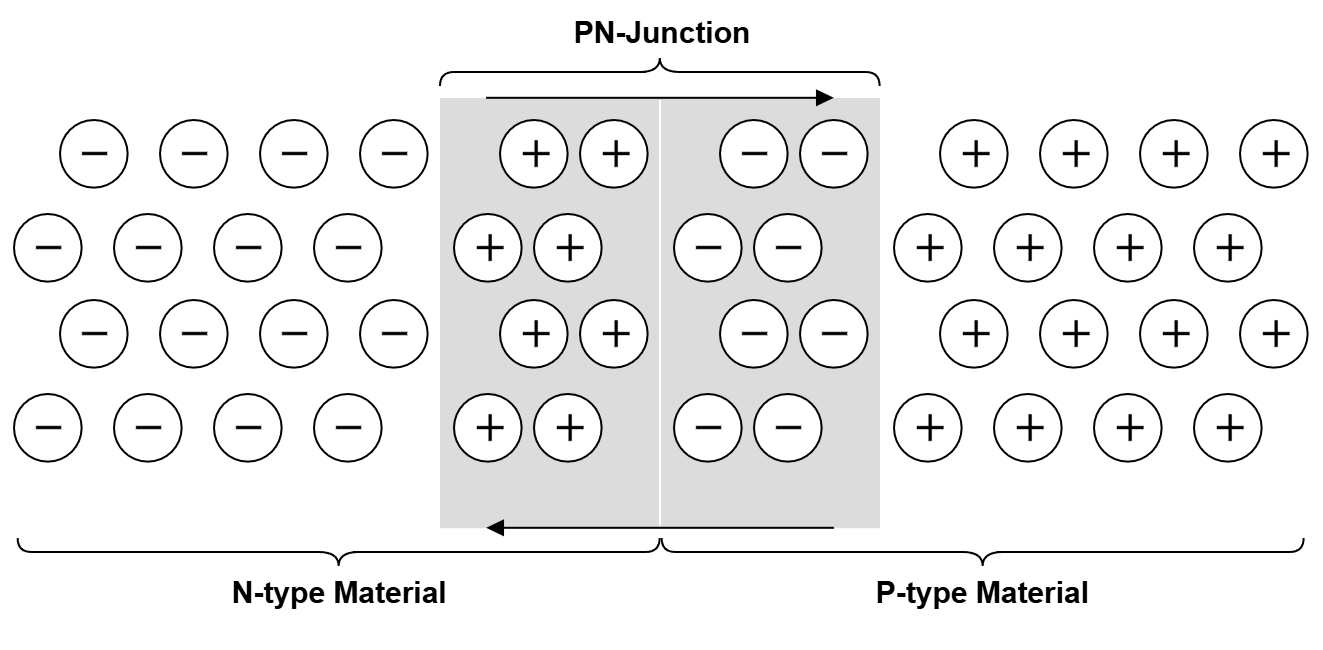
\includegraphics[width=\textwidth]{Sections/circuits/pn-junction.png}
  \caption{A PN-junction, where the depletion region is shown in gray.}
  \label{fig:pn-junction}
\end{figure}

\begin{Def}[MOSFET -- High-Level Overview]

    \label{def:mosfet_overview}
    \noindent
    A \textbf{MOSFET} (Metal-Oxide-Semiconductor Field-Effect Transistor) is a type of FET that uses its gate to control the flow of current.
    It consists of two default starting states:
    \begin{itemize}
      \item \textbf{Enhancement:} Normally \textbf{off} (i.e., no current flows), until such voltage is applied:
      \begin{itemize}
        \item \textbf{N-Channel Enhancement:} A positive voltage.
        \item \textbf{P-Channel Enhancement:} A negative voltage.
      \end{itemize}
      \item \textbf{Depletion:} Normally \textbf{on} (i.e., current flows), until such voltage is applied:
      \begin{itemize}
        \item \textbf{N-Channel Depletion:} A negative voltage.
        \item \textbf{P-Channel Depletion:} A positive voltage.
        \end{itemize}
    \end{itemize}
  \end{Def}

\newpage 

\begin{Def}[MOSFET -- Anatomy of N-Channel]

    \label{def:mosfet}

    A MOSFET \textbf{N-Channel Enhancement} is constructed as follows:
    \begin{itemize}
      \item \textbf{Substrate:} A base-layer of P-type material from which all parts will build upon.
      \item \textbf{Source \& Drain:} Two motes are dug at either ends of the substrate and filled with N-type material;
      One for our \textbf{source} and the other for our \textbf{drain}. Two metal contacts are placed on these motes (our terminals);
      A body of metal is connected to the bottom of the substrate (\textbf{base/body terminal}), which connects to the source terminal.
      \item \textbf{Gate:} A metal contact pad is placed between the motes on top of the SiO$_2$ layer, forming the \textbf{gate terminal}.
      A layer of silicon dioxide (SiO$_2$) is sandwiched between the gate and the substrate.
      Since SiO$_2$ is a superb insulator, it prevents the gate terminal from touching/interacting with the substrate.
      \item \textbf{Channeling:} SiO$_2$ is a \textbf{dielectric} material, meaning that when a charge is applied to one side, the opposite charge builds on the other side,
      creating an electric field. When a positive charge is applied, it attracts negative electrons from the other side, creating a \textbf{channel} (i.e., bridge)
      between the two motes (source to drain), allowing current.
    \end{itemize}
    
    \noindent
    The \textbf{M}etal from gates, the \textbf{O}xide from the SiO$_2$ layer, the \textbf{S}emiconductor from the substrate and motes, and 
    the \textbf{FET} from the field-effect, gives us the name \textbf{MOSFET}.

    \noindent
    \rule{\textwidth}{0.4pt}\\
    \noindent
    For \textbf{N-Channel Depletion}, A \emph{thin} N-type substrate-channel is already present, bridging the two motes (source and drain) together.
    Once a negative charge is applied to the gate, positive holes are attracted, weakening the channel; This effectively stops the flow of current.
\end{Def}

\vspace{-1em}
\begin{figure}[ht!]
  \centering
  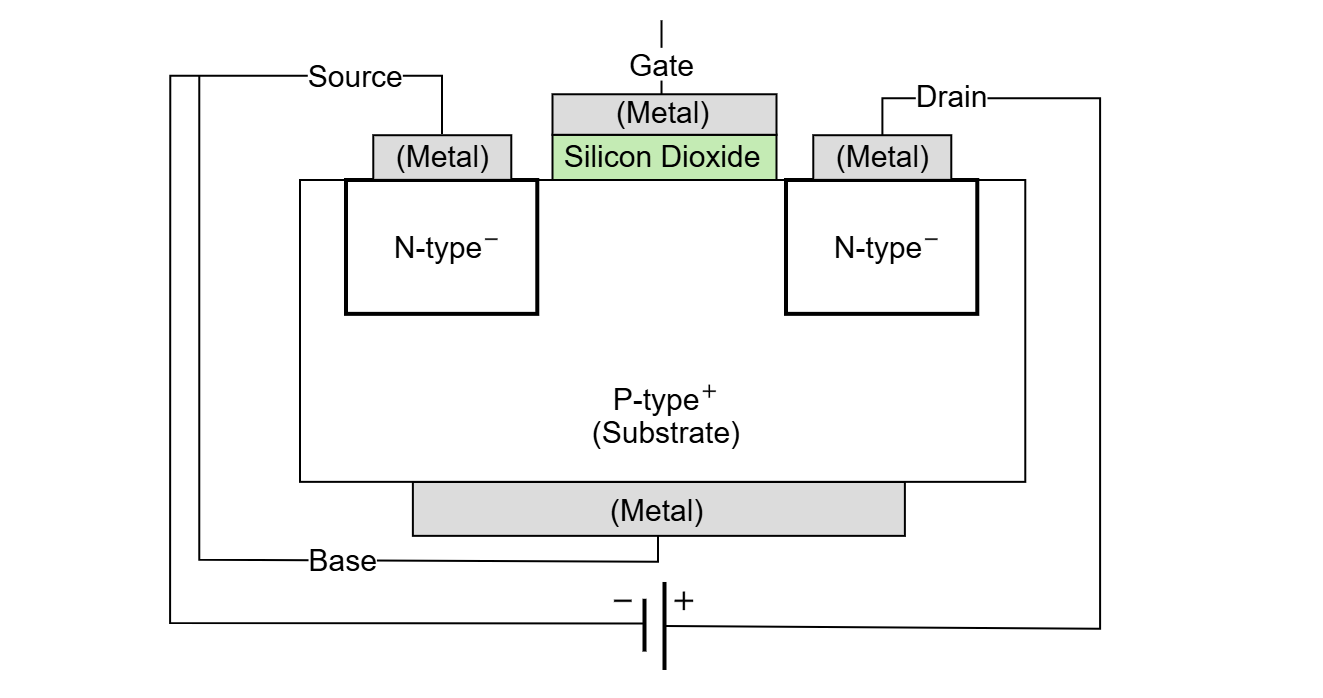
\includegraphics[width=.91\textwidth]{Sections/circuits/mosfet.png}
  \caption{N-Channel Enhancement (off). Negative battery side to source, positive to drain.}
  \label{fig:mosfet}
\end{figure}

\newpage

\begin{theo}[Flow of Electrons]

  \label{theo:flow_of_electrons}

  Recall that a body of electrons that are negatively charged (low potential), have a surplus of electrons.
  A positive charge (high potential) reflects a deficit of electrons. Therefore, when given the chance
  (alike water), electrons will flow to fill the void.
\end{theo}

\begin{Tip} An empty stomach has a high potential for food, while a full stomach has a low potential,
  as there's not much more room left to stuff food into.
\end{Tip}

\begin{Def}[MOSFET -- N-Channel Battery Configuration]

    \label{def:mosfet_gate_interaction}

    One battery is used to power the MOSFET, and another to control the gate.
    The source connects to the negative, and the drain to the positive side of the battery.
    
    The gate is connected to a second battery, which can be either positive or negative, depending on the MOSFET type.
    The \textbf{other} end of this battery is connected to the source terminal.
\end{Def}

\begin{figure}[ht!]
  \centering
  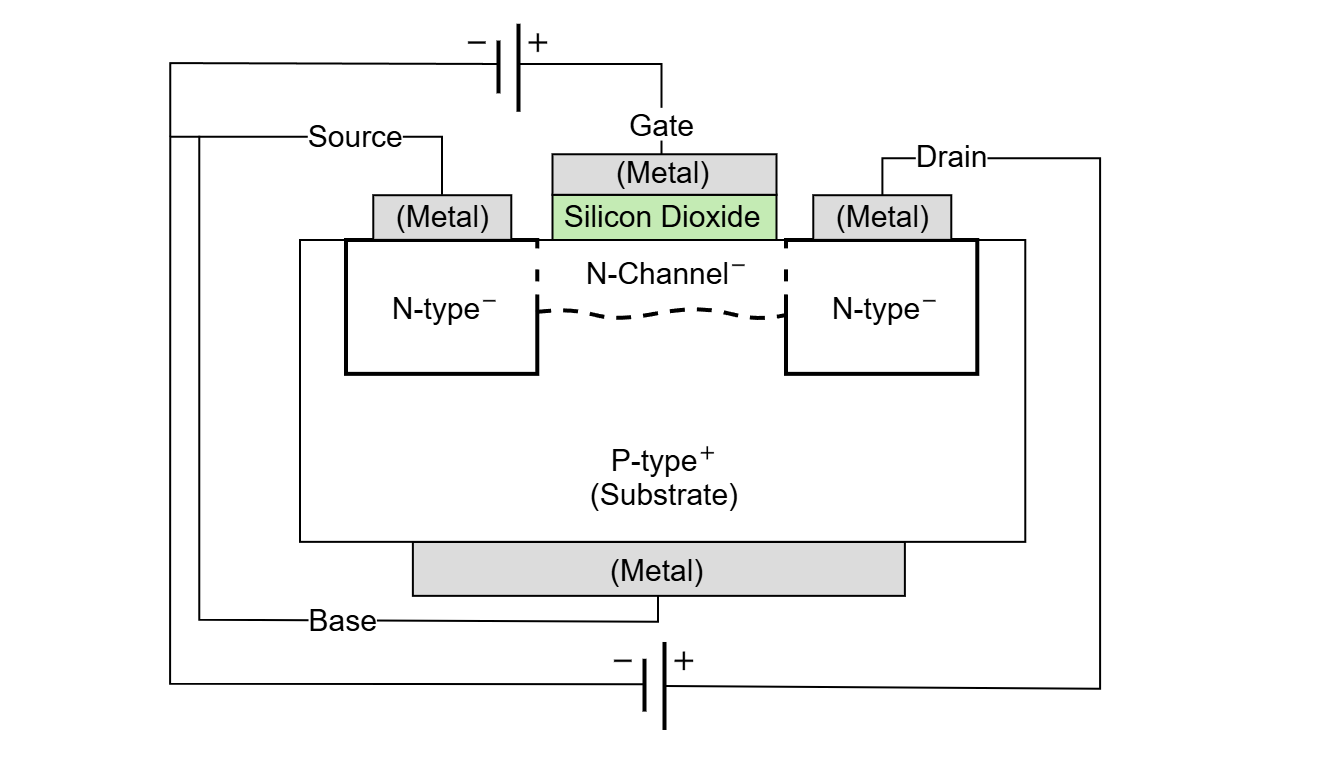
\includegraphics[width=.91\textwidth]{Sections/circuits/mosfet-on.png}
  \caption{N-Channel Enhancement (on). Negative battery side to gate, positive to source.
  Positive charge given to the gate attracts negative electrons on the other side of the 
  SiO$_2$ layer, creating a channel between the source and drain.}
  \label{fig:mosfet-on}
\end{figure}


% \begin{Tip} The same goes with heat, there technically is no such thing as the
%   ``cold'', it is just the lack of heat. At a high-level, heat is how fast atoms are jittering around.

%   Though for different reasons, heat rushes into the cold as it's ``jittery'' while the cold is ``still''.
%   Analogously, its relatively easier to run across a forest of trees than a field of dancing people; The chance
%   of bumping into someone knocking you off course than a tree is much higher.
% \end{Tip}

\newpage 

\begin{figure}[ht!]
  \centering
  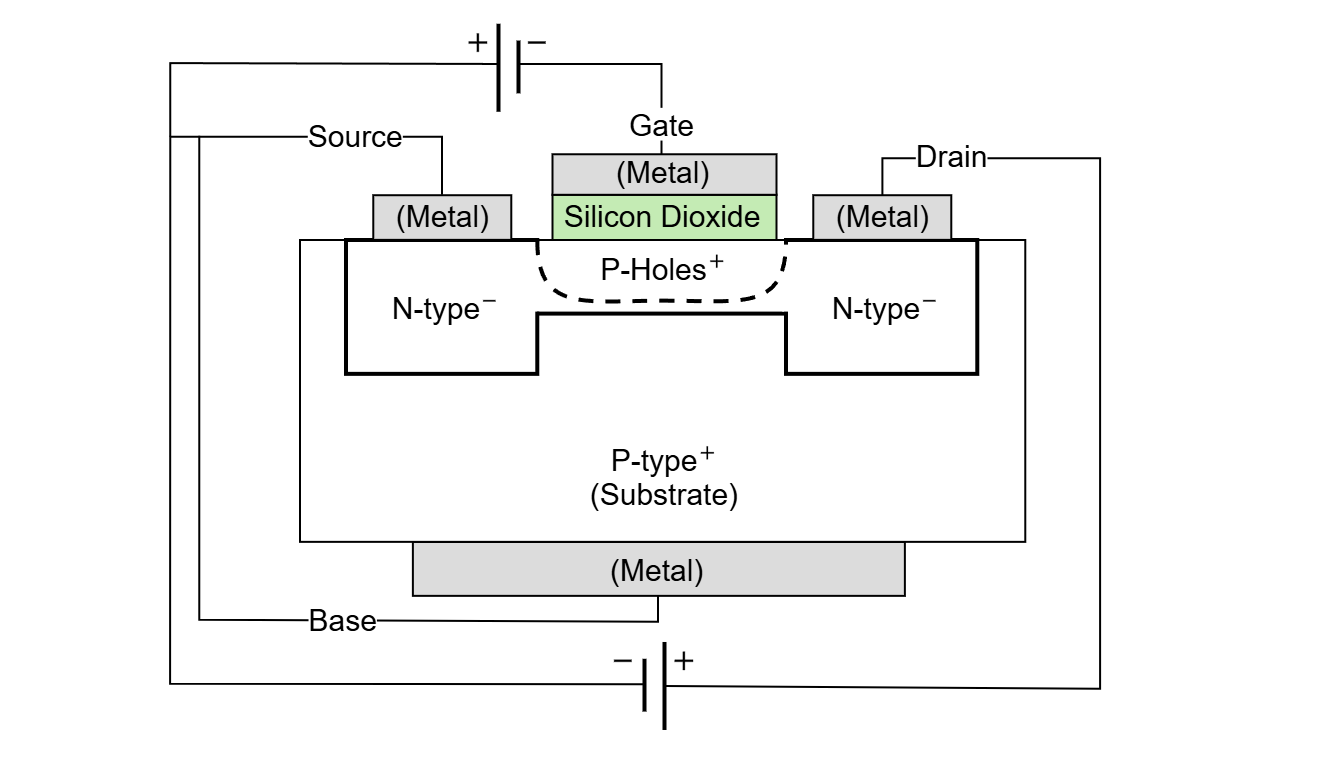
\includegraphics[width=.91\textwidth]{Sections/circuits/mosfet-depletion.png}
  \caption{N-Channel Depletion (on). Negative charge to gate, creates holes into the channel.}
  \label{fig:mosfet-depletion}
\end{figure}

\vspace{-1em}
\begin{Def}[MOSFET -- Anatomy of P-Channel]

    \label{def:mosfet_p_channel}

    The P-Channel variation follows the same logic as the N-Channel Definition (\ref{def:mosfet});
    Instead, we swap N-type for P-type materials, and vice versa. Then apply negative for Enhancement
    and positive for Depletion on the gate to open or close the channel respectively (\ref{def:mosfet_overview}).
    \textbf{In particular}, source now connects to a high potential and drain to a low potential.

\end{Def}

\vspace{-1em}
\begin{figure}[ht!]
  \centering
    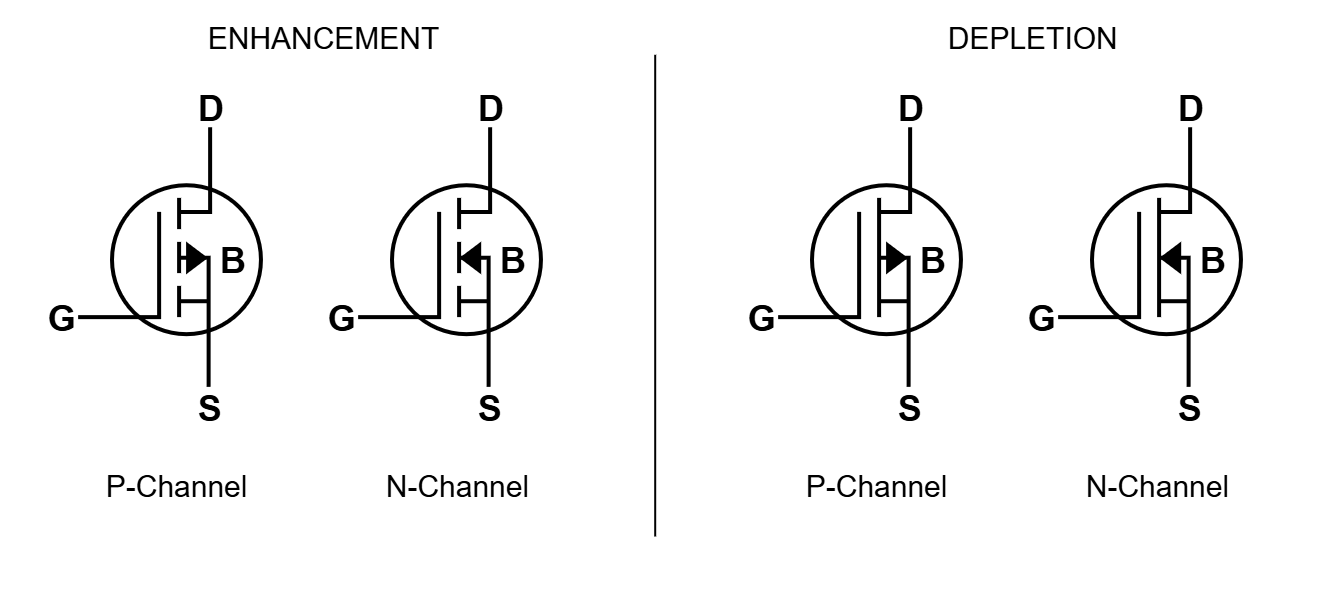
\includegraphics[width=.9\textwidth]{Sections/circuits/mosfet-symbol.png}
  \caption{MOSFET symbols, \textbf{G} (gate), \textbf{S} (source), \textbf{D} (drain), and \textbf{B} (body) terminals.}
  \label{fig:mosfet-symbol}
\end{figure}

\newpage 

\subsection{Logic Gates \& Functional Completeness}

\noindent
This section will cover how we take MOSFETs and use them to build logic gates.

\begin{Def}[Gate-Source Voltage $V_{GS}$]

  \label{def:gate_source_voltage}

  Recall Definition (\ref{def:mosfet_gate_interaction}), the gate battery's opposite end is connected to the source terminal.
  This serves as a zero-volt reference for the gate terminal.
  The difference in potential between the gate and source terminals is called the \textbf{gate-source voltage} ($V_{GS}$):
  \[
    V_{GS} = V_{G} - V_{S},
  \]
  
  \noindent
  Once $V_{GS}$ exceeds the threshold voltage $V_{TN}$ (for N-channel) or is below the threshold voltage $V_{TP}$ (for P-channel), the MOSFET turns on, allowing current to flow from source to drain.
\end{Def}

\begin{Tip} Notice that source takes from gate, i.e., for N-channel, the gate must overcome the source's 
  negative charge. Hence we must exceed a threshold voltage to turn on the MOSFET.
  For P-channel, the same logic applies, but in reverse, as the components are implemented in a complementary manner.
\end{Tip}

\begin{Def}[Pull-Up \& Pull-Down Switches]

  \label{def:pull_up_down_switches}

  Let $V_{DD}$ be the positive supply (“logical 1”) and ground (0 V) be “logical 0.”  A CMOS logic gate uses:
  \begin{itemize}
    \item \textbf{Pull-Down Switch} (Off: 0, On: 1): N-channel enhancement. If $V_{GS} > V_{TN}$, source connects to drain, producing a logical 1.
    \item \textbf{Pull-Up Switch} (Off: 1, On: 0): P-channel enhancement. If $V_{GS} < V_{TP}$, source connects to $V_{DD}$, producing a logical 1.
  \end{itemize}
\end{Def}
\begin{Tip} Think of pull-down as ``pulling down to the ground'' to allow electrons to escape.

  Additionally, the ``DD'' in $V_{DD}$ does not stand for anything; it was made not to be confused with 
  $V_D$, the voltage at the drain terminal. Though, unimaginative, it is simply convention.
\end{Tip}
\newpage 

\begin{Def}[CMOS Logic Gate]

  \label{def:cmos_logic_gate}

  A \textbf{CMOS logic gate} is a circuit that uses \textbf{C}omplementary \textbf{MOS}FETs to perform logical operations. It consists of:
  \begin{itemize}
    \item \textbf{Pull-Down Network (PDN):} N-channel MOSFETs (NFET) connected to ground.
    \item \textbf{Pull-Up Network (PUN):} P-channel MOSFETs (PFET) connected to $V_{DD}$.
  \end{itemize}
  
  \noindent
  The output is high when the PUN is active and the PDN is inactive, and vice versa.
\end{Def}

\vspace{-1em}
\begin{figure}[ht!]
  \centering
  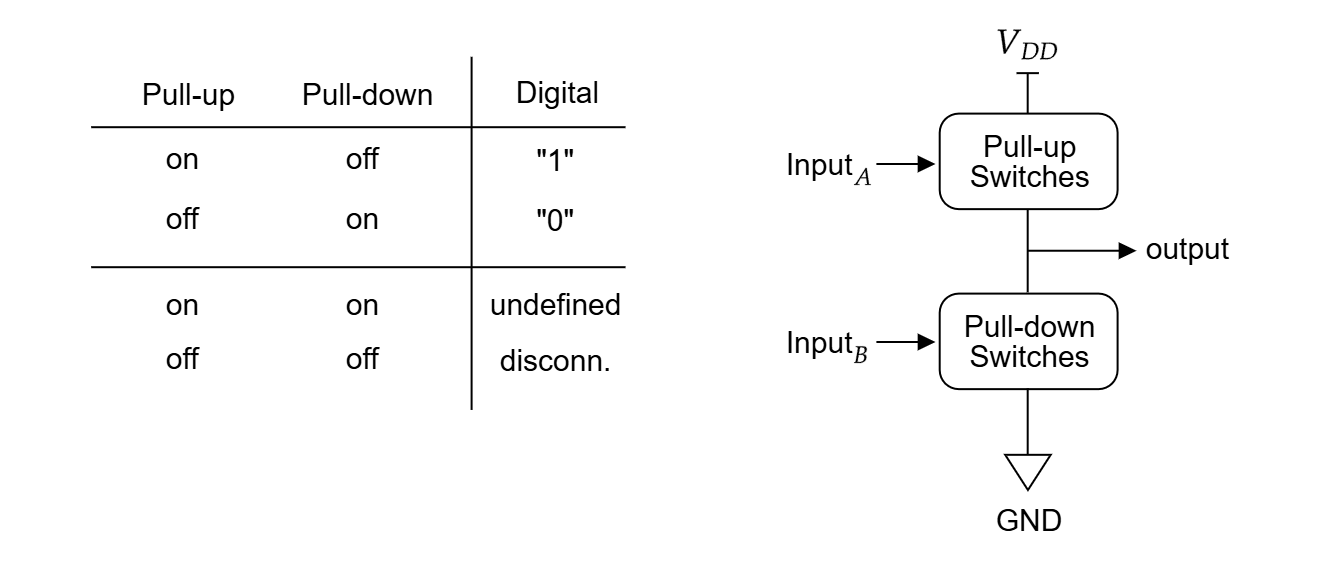
\includegraphics[width=\textwidth]{Sections/circuits/pun_pdn.png}
  \caption{Simple CMOS logic gate, where \textbf{GND} stands for ground, \textbf{$V_{DD}$} for positive supply.
  \textbf{Note:} That even if the circuit is disconnected, the output may still \emph{``remember''} its last state for some 
  time until the charge dissipates.}
  \label{fig:cmos-logic-gate}
\end{figure}

\begin{Def}[Simplified NFET \& PFET Symbols]

  \noindent
  Below are input gates $A$ and $B$, with two other terminals $T_1$ and $T_2$, simplifying Figure(\ref{fig:cmos-logic-gate}):

  \begin{center}
    
    
\includegraphics[width=\textwidth]{Sections/circuits/np_simp.png}
  \end{center}
  
  \noindent
  (1) NFET, $T_1$ output, and $T_2$ ground; (2) PFET, $T_1$ is $V_{DD}$ (typically 1V), and $T_2$ output \cite{youtube:1rZyGL1K5QI}.

\end{Def}

\newpage

\noindent
\begin{Def}[Open \& Closed Circuits -- NFET \& PFET Logic]

  \label{def:open_closed_circuits}

  A \textbf{closed circuit} is a complete path for current to flow, while an \textbf{open circuit} is an incomplete path:

  \begin{center}
  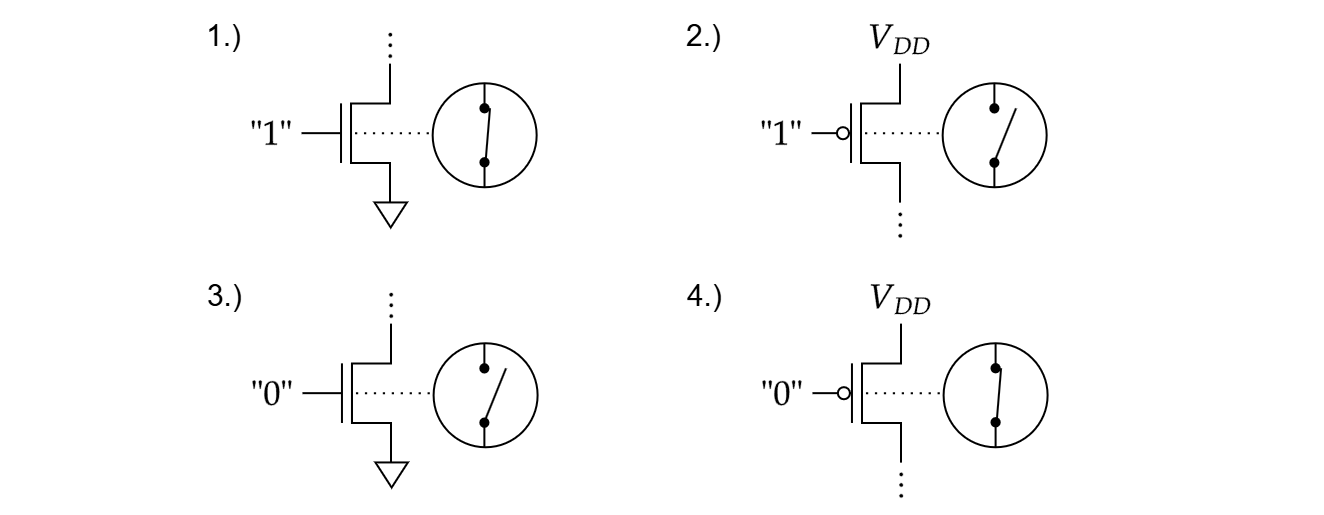
\includegraphics[width=\textwidth]{Sections/circuits/open_closed.png}
  \end{center}

  \noindent
  (1) An NFET is closed when given a digital 1 (high voltage), while (2) a PFET, is open;\\
  (3) NFET, open when given 0 (low voltage), while (4) a PFET is closed.
\end{Def}

\begin{Def}[MOSFET Logic Gate -- Not]

  \label{def:mosfet_logic_gate_not}

  Below shows a logic gate, NOT, using MOSFETs (NFET and PFET):

  \begin{center}
  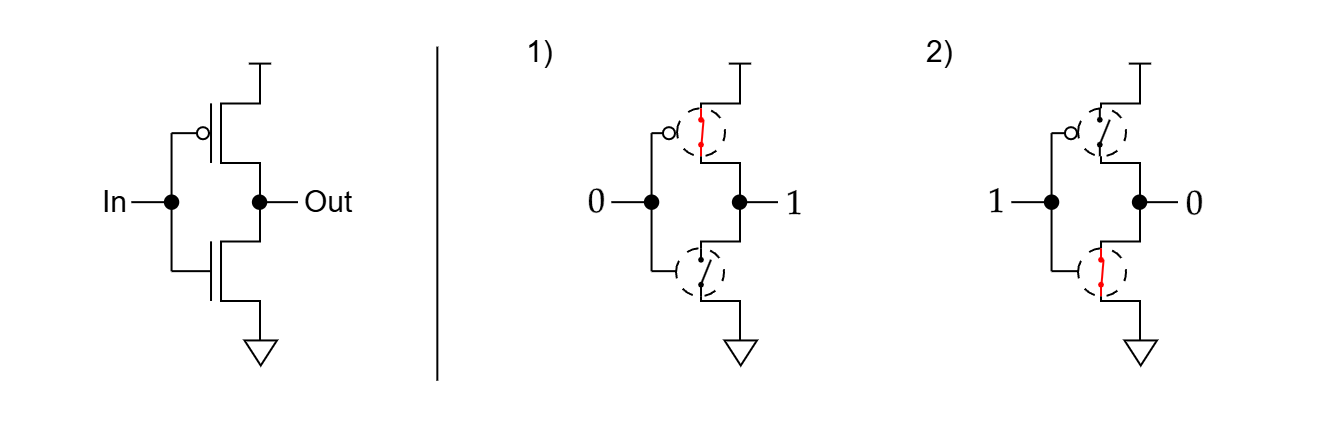
\includegraphics[width=\textwidth]{Sections/circuits/not.png}
  \end{center}

  \noindent
  Both the NFET and PFET share the same input. The top line represents $V_{DD}$ (positive supply), while the bottom line is ground (triangle).
  (1) input low, NFET is open, PFET is closed, output is high from $V_{DD}$; (2) input high, NFET is closed, PFET is open, output is low from ground.
  \textbf{Important:} A black dot connecting two or more lines represents a connection.
\end{Def}

\newpage 

\begin{Def}[Functional Completeness]

  \label{def:functional_completeness}

 it can be used to express all possible Boolean functions.
    For example, the set of operators $\{\text{AND, OR, NOT}\}$ is functionally complete.
    However, we can do better. The NAND gate (and NOR gate) by itself is functionally complete.
\end{Def}

\begin{Example}[Functionally Complete Sets of Operators]

    \begin{enumerate}
  \item $\{\mathrm{NAND}\}$ alone
    \begin{align*}
      \neg A &= A \operatorname{NAND} A,\\
      A\land B &= \neg\bigl(A \operatorname{NAND} B\bigr)
                = \bigl(A \operatorname{NAND} B\bigr)\operatorname{NAND}\ \bigl(A \operatorname{NAND} B\bigr),\\
      A\lor B  &= (A \operatorname{NAND} A)\operatorname{NAND}\ (B \operatorname{NAND} B).
    \end{align*}

  \item $\{\mathrm{NOR}\}$ alone
    \begin{align*}
      \neg A &= A \operatorname{NOR} A,\\
      A\lor B  &= \neg\bigl(A \operatorname{NOR} B\bigr)
                = \bigl(A \operatorname{NOR} B\bigr)\operatorname{NOR}\ \bigl(A \operatorname{NOR} B\bigr),\\
      A\land B &= (A \operatorname{NOR} A)\operatorname{NOR}\ (B \operatorname{NOR} B).
    \end{align*}

    \item $\{\land,\neg\}$ alone
    \begin{align*}
      \neg A   &= \neg A,\\
      A\land B &= A\land B,\\
      A\lor B  &= \neg\bigl(\neg A \land \neg B\bigr).
    \end{align*}

  \item $\{\lor,\neg\}$ alone
    \begin{align*}
      \neg A   &= \neg A,\\
      A\lor B  &= A\lor B,\\
      A\land B &= \neg\bigl(\neg A \lor \neg B\bigr).
    \end{align*}

  \item $\{\to,\neg\}$ alone
    \begin{align*}
      \neg A   &= \neg A,\\
      A\lor B  &= \neg A \to B,\\
      A\land B &= \neg\bigl(A \to \neg B\bigr).
    \end{align*}
\end{enumerate}

\noindent
Recall, $A \to B$ is logically equivalent to $\neg A \lor B$. 
\end{Example}

\newpage 

\noindent
Let's brainstorm possibilities for an AND and NAND, and elaborate on Defintition (\ref{def:cmos_logic_gate}):
\begin{theo}[Balancing Series \& Parallel Connections]

  \label{theo:balancing_series_parallel}

    \noindent
    It's important in a CMOS circuit that the PUN and PDN are in fact complements of each other. Below
    illustrates two types of connections:

    \begin{center}
      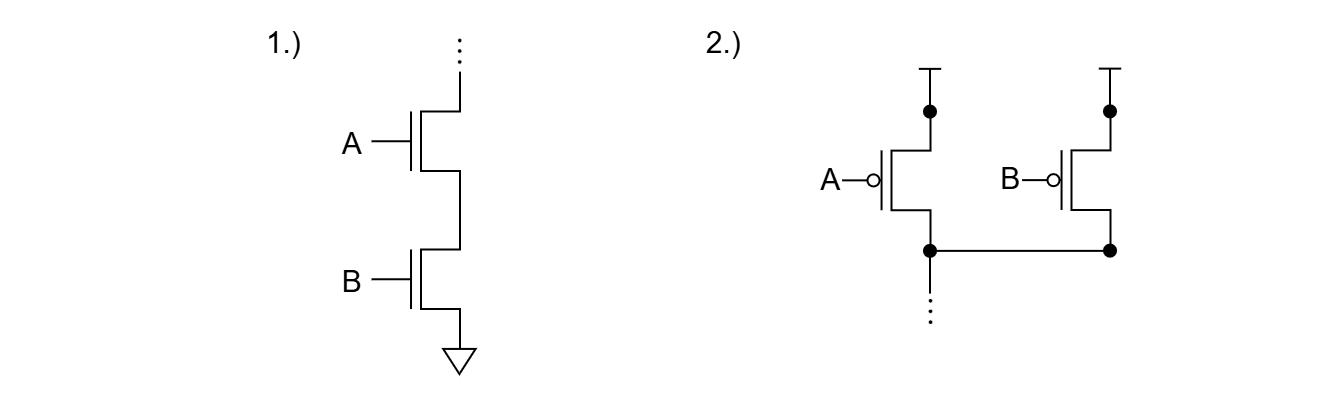
\includegraphics[width=\textwidth]{Sections/circuits/np_comp.png}
    \end{center}

    \noindent
    (1) Shows a NFET \textbf{series} connection (i.e., sequentially connected). Theoretically in isolation, this represents
    an AND gate ($A \cdot B$), meaning both $A$ and $B$ must be high to close the circuit. 
    
    (2) Shows a PFET in \textbf{parallel} connection (i.e., side-by-side connected). As per complementarity, this represents the NAND gate
    ($\overline{A} + \overline{B} = \overline{A \cdot B}$), by De Morgan's Law; Either $A$ or $B$ must be low to close the circuit.\\
    \rule{\textwidth}{0.4pt}\\
    \noindent
    Hence to \textbf{balance}, between the PUN and PDN, we must ensure that:
    \begin{itemize}
        \item each NFET series requires a PFET parallel.
        \item each PFET series requires a NFET parallel.
    \end{itemize}

    \noindent
    This keeps our networks complementary, ensuring that \underline{when one is closed, the other is open}.
\end{theo}

\begin{Tip} Think about how to create this before moving to the next page.
  understand that the placement of the output determines the logic of the circuit. 
  Since PUNs default to high, think about how that might affect the output.

  In CMOS, there must be both a PUN and PDN, think about how to balance the (2), from the above Theorem (\ref{theo:balancing_series_parallel}), to create a NAND gate.
\end{Tip}



\newpage
\begin{theo}[CMOS Logic Gate -- NAND]

  \label{def:mosfet_logic_gate_nand}

  \noindent
  Combining both networks in Theorem (\ref{theo:balancing_series_parallel}) yields a NAND gate in the following configuration:

  \begin{center}
    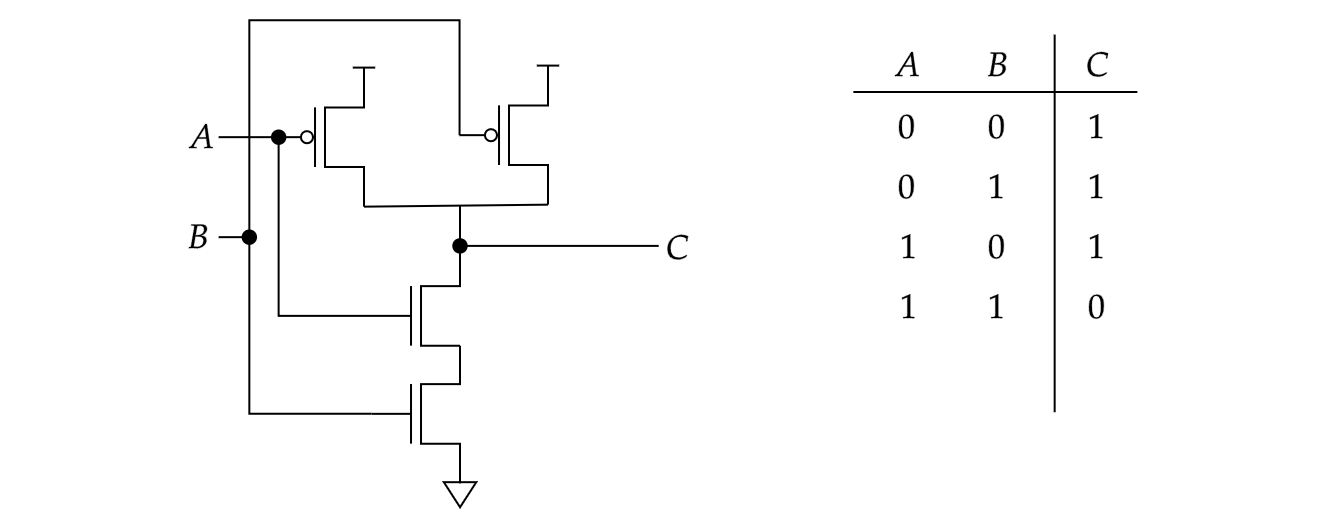
\includegraphics[width=\textwidth]{Sections/circuits/nand.png}
  \end{center}
\end{theo}

\vspace{2em}
\begin{figure}[ht!]
  \centering
  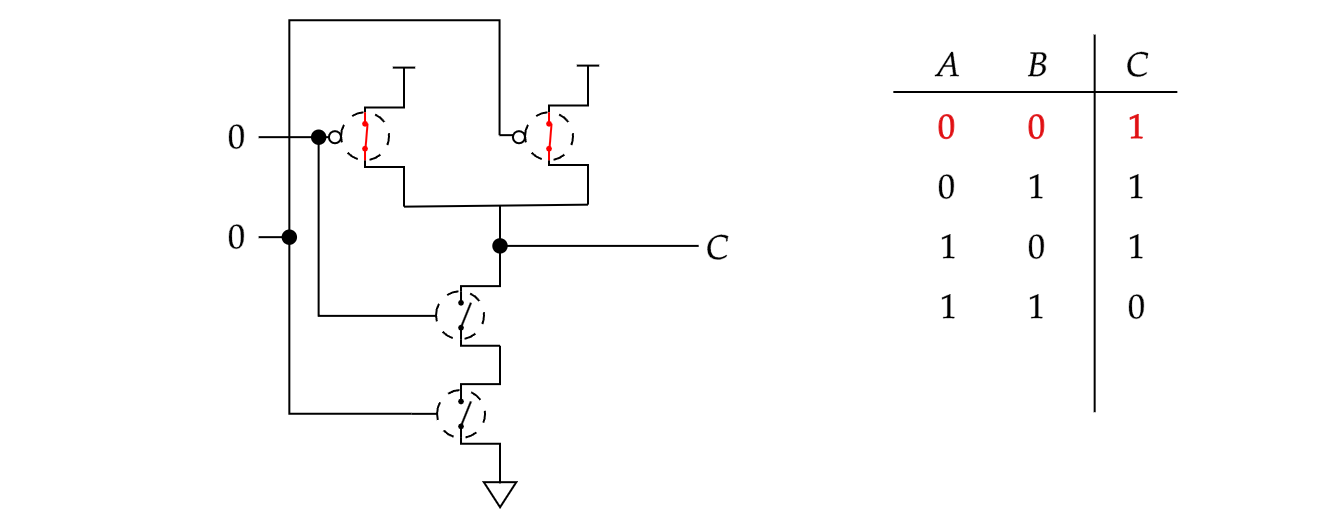
\includegraphics[width=\textwidth]{Sections/circuits/nand_1.png}
  \caption{Both inputs are (0,0), PUN closed, PDN open, hence the output is high (1).}
  \label{fig:nand-1}
\end{figure}

\begin{figure}[ht!]
  \centering
  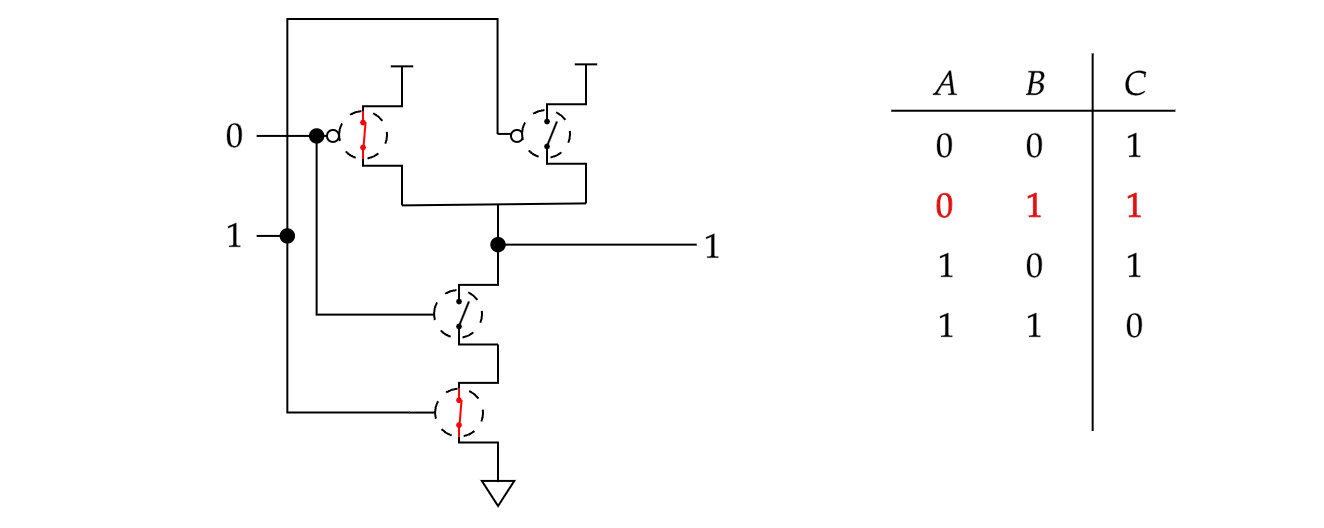
\includegraphics[width=\textwidth]{Sections/circuits/nand_2.png}
  \caption{Both inputs are (0,1), PUN half-closed reaching the output, PDN half-closed, but can't reach the output; Hence the output is high (1).}
  \label{fig:nand-2}
\end{figure}



% \chapter{Proving Algorithms}
% \section{Stable Matchings}

In proving the correctness of algorithms we introduce the stable matching problem.
A combinatorial optimization problem that seeks to find the best possible matching between two sets of elements.
When we say ``best possible matching,'' we mean that the matching is stable, and that there is no other matching that is better.

\begin{Def}[Stable Matching]

    A matching is \textbf{stable} if there is no pair of elements that prefer each other over their current match.
\end{Def}

\begin{Def}[Unstable Matching]

    A matching is \textbf{unstable} if there is a pair of elements that prefer each other over their current match.
\end{Def}

\noindent
I.e., in verifying a stable matching, if any one pair of elements switch partners, the matching is unstable. If no pairs swap, the matching is stable.

\subsection*{Scenario: \textit{Lunch Time}}
Imagine it's lunch time at elementary school, and a group of kids $E=$\{Ena, Eda\} swap lunches with $A=$\{Ava, Adi\}.
They each have a list of preferences from favorite to least favorite. We visualize the following preferences:

\begin{table}[h!]
    \centering
    \begin{tabular}{c|c|c|}
    \multicolumn{3}{c}{\textbf{E's Preference List}} \\ \cline{2-3}
    \cline{2-3}
    \rowcolor{OliveGreen!10} 
    \cellcolor{white}           & 1st       & 2nd  \\  \hline   
    \multicolumn{1}{|>{\columncolor{OliveGreen!10}}c|}{Ena}    & Ava     & Adi    \\
    \multicolumn{1}{|>{\columncolor{OliveGreen!10}}c|}{Eda}      & Ava     & Adi   \\ \hline
    \end{tabular}
    \quad
    \begin{tabular}{c|c|c|}
    \multicolumn{3}{c}{\textbf{A's Preference List}} \\ \cline{2-3}
    \cline{2-3}
    \rowcolor{OliveGreen!10} 
    \cellcolor{white}           & 1st       & 2nd\\ \hline
    \multicolumn{1}{|>{\columncolor{OliveGreen!10}}c|}{Ava}   & Ena     & Eda    \\
    \multicolumn{1}{|>{\columncolor{OliveGreen!10}}c|}{Adi}     & Ena   & Eda \\ \hline
    \end{tabular}
\end{table}

\newpage

\noindent
Observe the following matchings:\\

\noindent
(1.) Pairs, Ena-Ava, Eda-Adi swapped lunches.
\begin{table}[h!]
    \centering
    \begin{tabular}{c|c|c|}
    \multicolumn{3}{c}{\textbf{E's Preference List}} \\ \cline{2-3}
    \cline{2-3}
    \rowcolor{OliveGreen!10} 
    \cellcolor{white}           & 1st       & 2nd  \\  \hline   
    \multicolumn{1}{|>{\columncolor{OliveGreen!10}}c|}{Ena}    & \cellcolor{purple!15}Ava     & Adi    \\
    \multicolumn{1}{|>{\columncolor{OliveGreen!10}}c|}{Eda}      & Ava     & \cellcolor{purple!15}Adi   \\ \hline
    \end{tabular}
    \quad
    \begin{tabular}{c|c|c|}
    \multicolumn{3}{c}{\textbf{A's Preference List}} \\ \cline{2-3}
    \cline{2-3}
    \rowcolor{OliveGreen!10} 
    \cellcolor{white}           & 1st       & 2nd\\ \hline
    \multicolumn{1}{|>{\columncolor{OliveGreen!10}}c|}{Ava}   & \cellcolor{purple!15}Ena     & Eda    \\
    \multicolumn{1}{|>{\columncolor{OliveGreen!10}}c|}{Adi}     & Ena   & \cellcolor{purple!15} Eda \\ \hline
    \end{tabular}
\end{table}

\noindent
 This matching is \textbf{stable}. Ena and Ava prefer each other's lunches. Eda will ask Ava to trade, and Ava will refuse because she prefers Ena's lunch. Adi does the same with Ena, but they also refuse.
\begin{Tip}
    If it's hard to keep track who is who, here's a possible order to read in: Ena got Ava, and Ena is their 1st choice. 
    Eda got Adi, and Eda is their 2nd choice.
\end{Tip}
\noindent
Changing the preference tables,\\

\noindent
(2.) Pairs, Ena-Adi, Eda-Ava swapped lunches.

\begin{table}[h!]
    \centering
    \begin{tabular}{c|c|c|}
    \multicolumn{3}{c}{\textbf{E's Preference List}} \\ \cline{2-3}
    \cline{2-3}
    \rowcolor{OliveGreen!10} 
    \cellcolor{white}           & 1st       & 2nd  \\  \hline   
    \multicolumn{1}{|>{\columncolor{OliveGreen!10}}c|}{Ena}    & Ava     & \cellcolor{purple!15}Adi    \\
    \multicolumn{1}{|>{\columncolor{OliveGreen!10}}c|}{Eda}      & Adi     & \cellcolor{purple!15}Ava   \\ \hline
    \end{tabular}
    \quad
    \begin{tabular}{c|c|c|}
    \multicolumn{3}{c}{\textbf{A's Preference List}} \\ \cline{2-3}
    \cline{2-3}
    \rowcolor{OliveGreen!10} 
    \cellcolor{white}           & 1st       & 2nd\\ \hline
    \multicolumn{1}{|>{\columncolor{OliveGreen!10}}c|}{Ava}   & Ena     & Eda \cellcolor{purple!15}    \\
    \multicolumn{1}{|>{\columncolor{OliveGreen!10}}c|}{Adi}     & Ena  \cellcolor{purple!15} &  Eda \\ \hline
    \end{tabular}
\end{table}

\noindent
This matching is $\textbf{unstable}$. Ena and Ava would rather eat each other's lunches.\\
\begin{Def}[Unique Stable Matching]

    A matching is \textbf{uniquely stable} if between two sets of elements, there is only one possible stable matching.
\end{Def}
\noindent
\textbf{Example:} If everyone uniquely prefers each other, there is only one stable matching.\\
\newpage 
\noindent
(3.) Pairs, Ena-Ava, Eda-Adi swapped lunches.
\begin{table}[h!]
    \centering
    \begin{tabular}{c|c|c|}
    \multicolumn{3}{c}{\textbf{E's Preference List}} \\ \cline{2-3}
    \cline{2-3}
    \rowcolor{OliveGreen!10} 
    \cellcolor{white}           & 1st       & 2nd  \\  \hline   
    \multicolumn{1}{|>{\columncolor{OliveGreen!10}}c|}{Ena}    & \cellcolor{purple!15}Ava     & Adi    \\
    \multicolumn{1}{|>{\columncolor{OliveGreen!10}}c|}{Eda}      & \cellcolor{purple!15}Adi     & Ava   \\ \hline
    \end{tabular}
    \quad
    \begin{tabular}{c|c|c|}
    \multicolumn{3}{c}{\textbf{A's Preference List}} \\ \cline{2-3}
    \cline{2-3}
    \rowcolor{OliveGreen!10} 
    \cellcolor{white}           & 1st       & 2nd\\ \hline
    \multicolumn{1}{|>{\columncolor{OliveGreen!10}}c|}{Ava}   & Ena \cellcolor{purple!15}     & Eda     \\
    \multicolumn{1}{|>{\columncolor{OliveGreen!10}}c|}{Adi}     & Eda  \cellcolor{purple!15} &  Ena \\ \hline
    \end{tabular}
\end{table}

\noindent
This matching is a \textbf{unique stable matching}. If rather Ena-Adi and Eda-Ava (2nd-choice parings), then both pairs would end up swapping to their 1st-choice. \textbf{Notably}: for table sizes of $n\times n$, then \underline{$0<n\leq 2$ \textbf{forces a unique stable matching.}}

\section{Gale-Shapley Algorithm}

\noindent
We will now introduce the Gale-Shapley algorithm, for which we will prove its correctness, time complexity, and space complexity.

\begin{theo}[Gale-Shapley Algorithm]

    The \textbf{Gale-Shapley algorithm} is a method for finding a stable matching between two sets of elements. It is also known as the \textbf{Deferred Acceptance Algorithm}.\\

    \noindent
\textbf{Algorithm:}
    Given sets $E={e_1,\dots,e_n}$ and $A={a_1,\dots,a_n}$. Then find a stable matching:
    \begin{enumerate}
        \item [(i.)] Each $e_i\in E$ proposes to their most preferred $a_j$.
        \item [(ii.)] For each $a_j\in A$:
        \begin{enumerate}
            \item [(a.)] If $a_j$ is free, they accept the proposal.
            \item [(b.)] If $a_j$ is already matched, $a_j$ either accepts or rejects. If $a_j$ accepts, the previous match is broken.
        \end{enumerate}
    \end{enumerate}
    \noindent
    Each $e_i$ continues to propose to their next most preferred $a_j$ until all $e_i$ are matched.\\

    \noindent
    \textbf{Claims:}
    \begin{enumerate}
        \item At least one stable matching is guaranteed.
        \item Unless the table is unique, the proposing will always get their best choice unless it conflicts with another proposer.
    \end{enumerate}
\end{theo}
\noindent
First we will prove the correctness, then implement the algorithm and analyze its time and space complexity.

\newpage

\begin{Proof}[Gale-Shapley Algorithm Correctness]

    \textbf{Claim 1:} Suppose, for sake of contradiction, that some $a_j \in A$ is not matched upon termination of the algorithm.
    Then some $e_i \in E$ is also not matched assuming $|E| = |A|$. Then $e_i$ must have not proposed to $a_j$, contradicting
    that $e_i$ proposed to all elements of $A$. Thus, the program only terminates when all $e_i$ are matched.\\

    \noindent
    \textbf{Claim 2:} Suppose $E$ proposes to $A$ with unique first choices. Then all $a_i\in A$ must accept their first proposal.
    Now suppose $e_i,e_j\in E$ have a conflicting choice $a_i$. Then $a_i$ gets their preference only in that case. 
    
\end{Proof}
\begin{Func}[Gale-Shapley Algorithm - \texttt{GS(E,A)}]
    Finds a stable matching between two sets of elements:

    \vspace{.5em}
    \noindent
    \textbf{Input:} Two sets, $E$ and $A$, of equal size.\\
    \textbf{Output:} A stable matching between $E$ and $A$.\\
    \begin{algorithm}[H]
        \SetAlgoLined
        \SetKwProg{Fn}{Function}{:}{\KwRet{Matching $M$}}
        \Fn{\texttt{GS(E,A)}}{
            $M \gets \emptyset$\;
            \While{there is some unmatched element in $E$}{
                $e \gets$ next unmatched element in $E$\;
                $a \gets$ next avalaible preferred choice of $e$\;
                \If{$a$ is not yet matched}{
                    match $e$ and $a$\;
                    add the pair $(e, a)$ to $M$\;
                }
                \Else{
                    \If{$a$ prefers $e$ over their current match}{
                        match $e$ and $a$, replacing the current match\;
                        update $M$ accordingly\;
                    }
                }
            }
            \KwRet{$M$}\;
        }
    \end{algorithm}

    \noindent
    \textbf{Time Complexity:} $O(n^2)$ time, where $n$ is the number of elements in $E$ and $A$. Worst-case,
    each element in $E$ proposes to each element in $A$, i.e., $n\cdot n$ combinations to check.\\

    \noindent
    \textbf{Space Complexity:} $O(n^2)$ space, where we store $|E|\cdot|A|=n\cdot n$ pairs.
\end{Func}



% \chapter{Graphs and Trees}
% \section{Paths and Connectivity}
Graphs are similar to train networks or airline routes. They connect one 
location to another.

\begin{Def}[Graph]

    A \textbf{graph} is a collection of points, called \textbf{vertices} or \textbf{nodes}, 
    connected by lines, called \textbf{edges}. Similarly to how a polygon has vertices connected by edges.

\end{Def}
\begin{Def}[Undirected Graph]

    An \textbf{undirected graph} is a graph where the edges have no particular direction going both ways between nodes. 
    A \textbf{degree} of a node is the number of edges connected to it.
\end{Def}
\noindent
\textbf{Example:} Figure (\ref{fig:undir_graph}) shows an undirected graph:\\
\begin{figure}[h]
    \begin{center}
      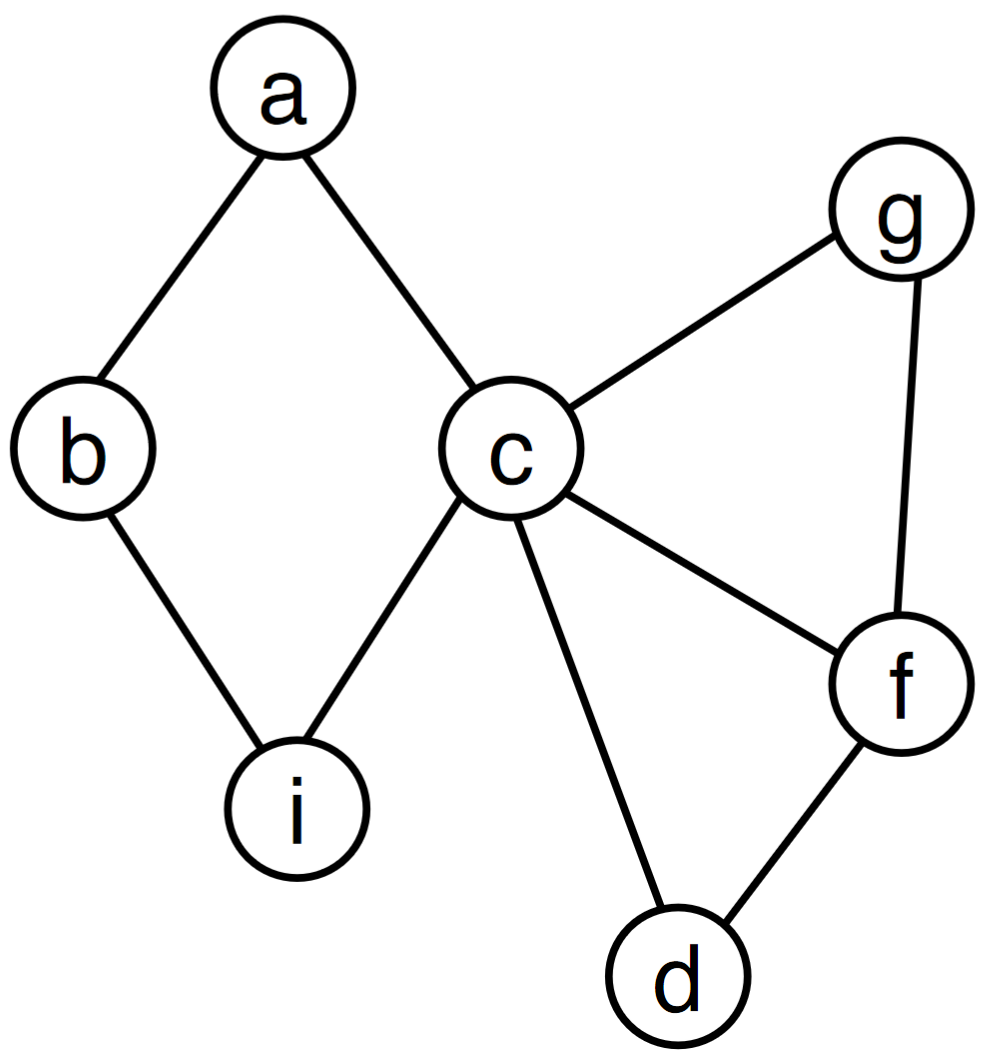
\includegraphics[height=1.8in]{./Sections/graphs/undir_graph.png}
    \end{center}
     \caption{An undirected graph with 7 vertices and 9 edges.}\label{fig:undir_graph}
  \end{figure}

\noindent
Node $a$ has a degree of 2, and node $c$ has a degree of 5.\\
\newpage

\begin{Def}[Directed Graph]

    A \textbf{directed graph} is where the edges have a specific direction from one node to another.
    \begin{itemize}
        \item  The \textbf{indegree} of a node is the number of edges that point to it.
        \item The \textbf{outdegree} of a node is the number of edges that point from it.
    \end{itemize}
\end{Def}
\noindent
\textbf{Example:} Figure (\ref{fig:dir_graph}) shows a directed graph:\\
\begin{figure}[h]
    \begin{center}
      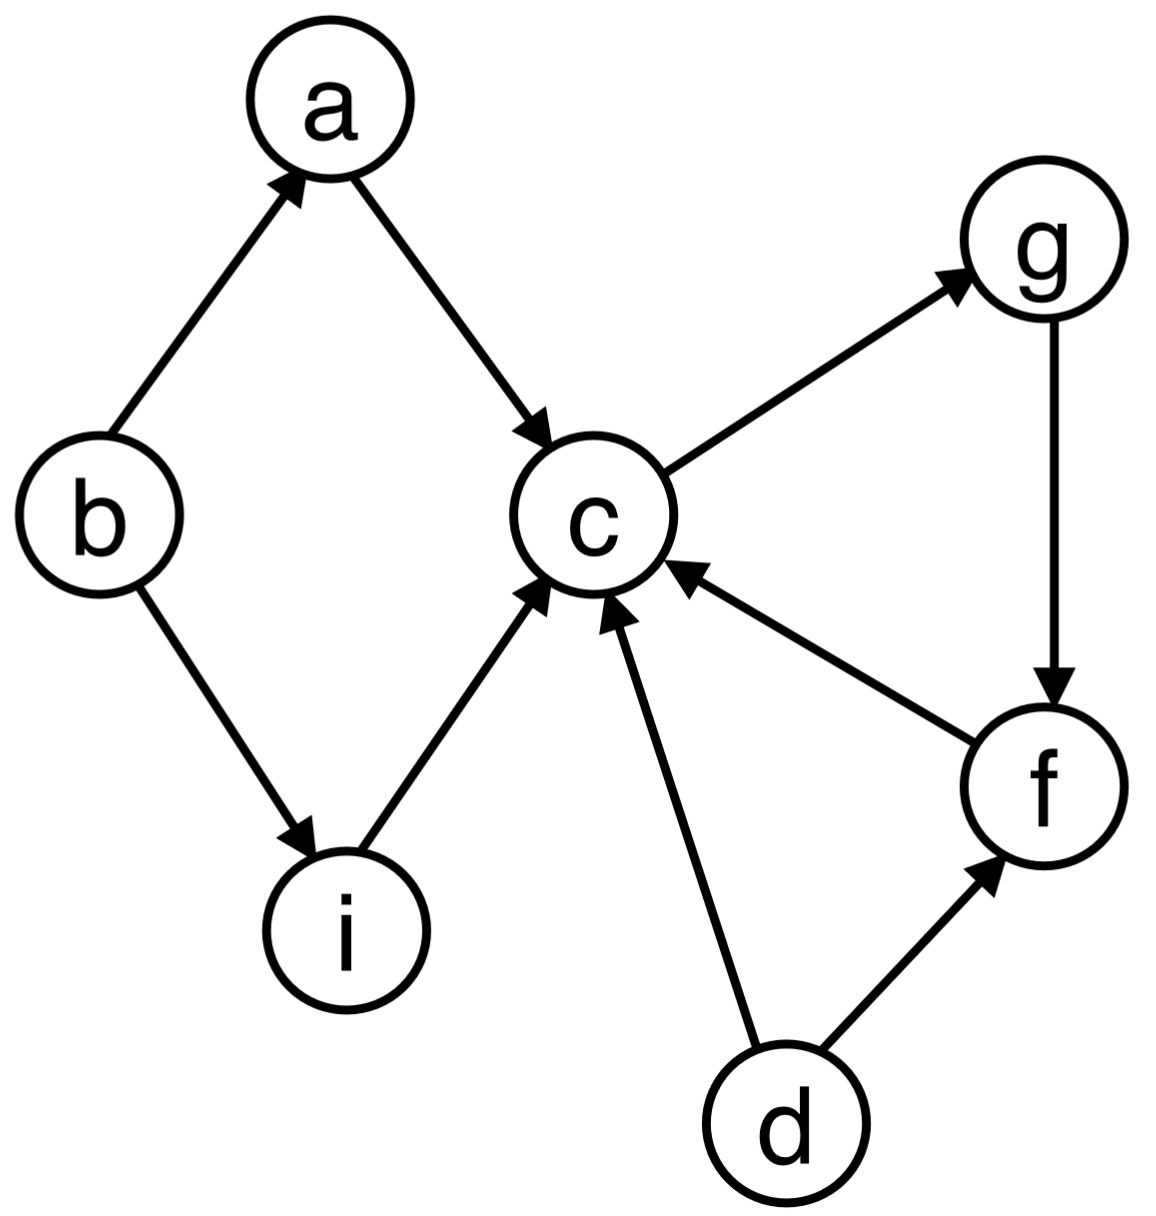
\includegraphics[height=1.5in]{./Sections/graphs/dir_graph.png}
    \end{center}
     \caption{A directed graph with 7 vertices and 9 edges.}\label{fig:dir_graph}
  \end{figure}

  \noindent
    Node $b$ has an outdegree of 2 and an indegree of 0. $c$ has an indegree of 4 and an outdegree of 1.

\begin{Def}[Weighted Graph]

    A \textbf{weighted graph} is a graph where each edge has a numerical value assigned to it.
\end{Def}
\noindent
\textbf{Example:} Figure (\ref{fig:weight_graph}) shows a weighted graph:\\
\begin{figure}[h]
    \begin{center}
      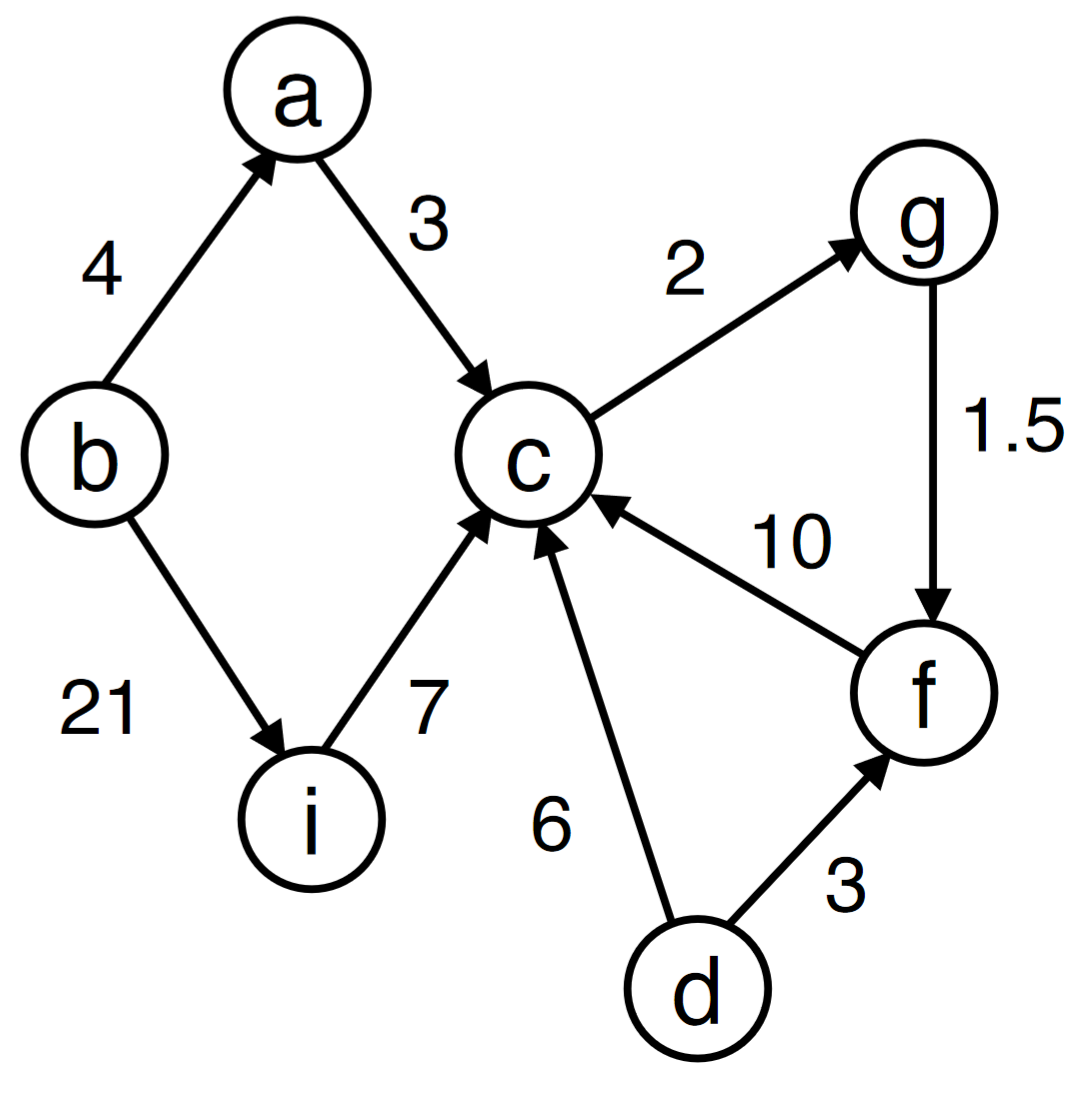
\includegraphics[height=1.5in]{./Sections/graphs/weight_graph.png}
    \end{center}
     \caption{A weighted graph with 7 vertices and 9 edges.}\label{fig:weight_graph}
  \end{figure}
\newpage
\begin{Def}[Path]

    A \textbf{path} is a sequence of edges that connect a sequence of vertices. A 
    path is \textbf{simple} if all nodes are distinct.
\end{Def}

\noindent
\textbf{Example:} In Figure (\ref{fig:path_graph}), a simple path $h\leftrightarrow b \leftrightarrow i \leftrightarrow c \leftrightarrow d$ is shown:\\
\begin{figure}[h]
    \begin{center}
      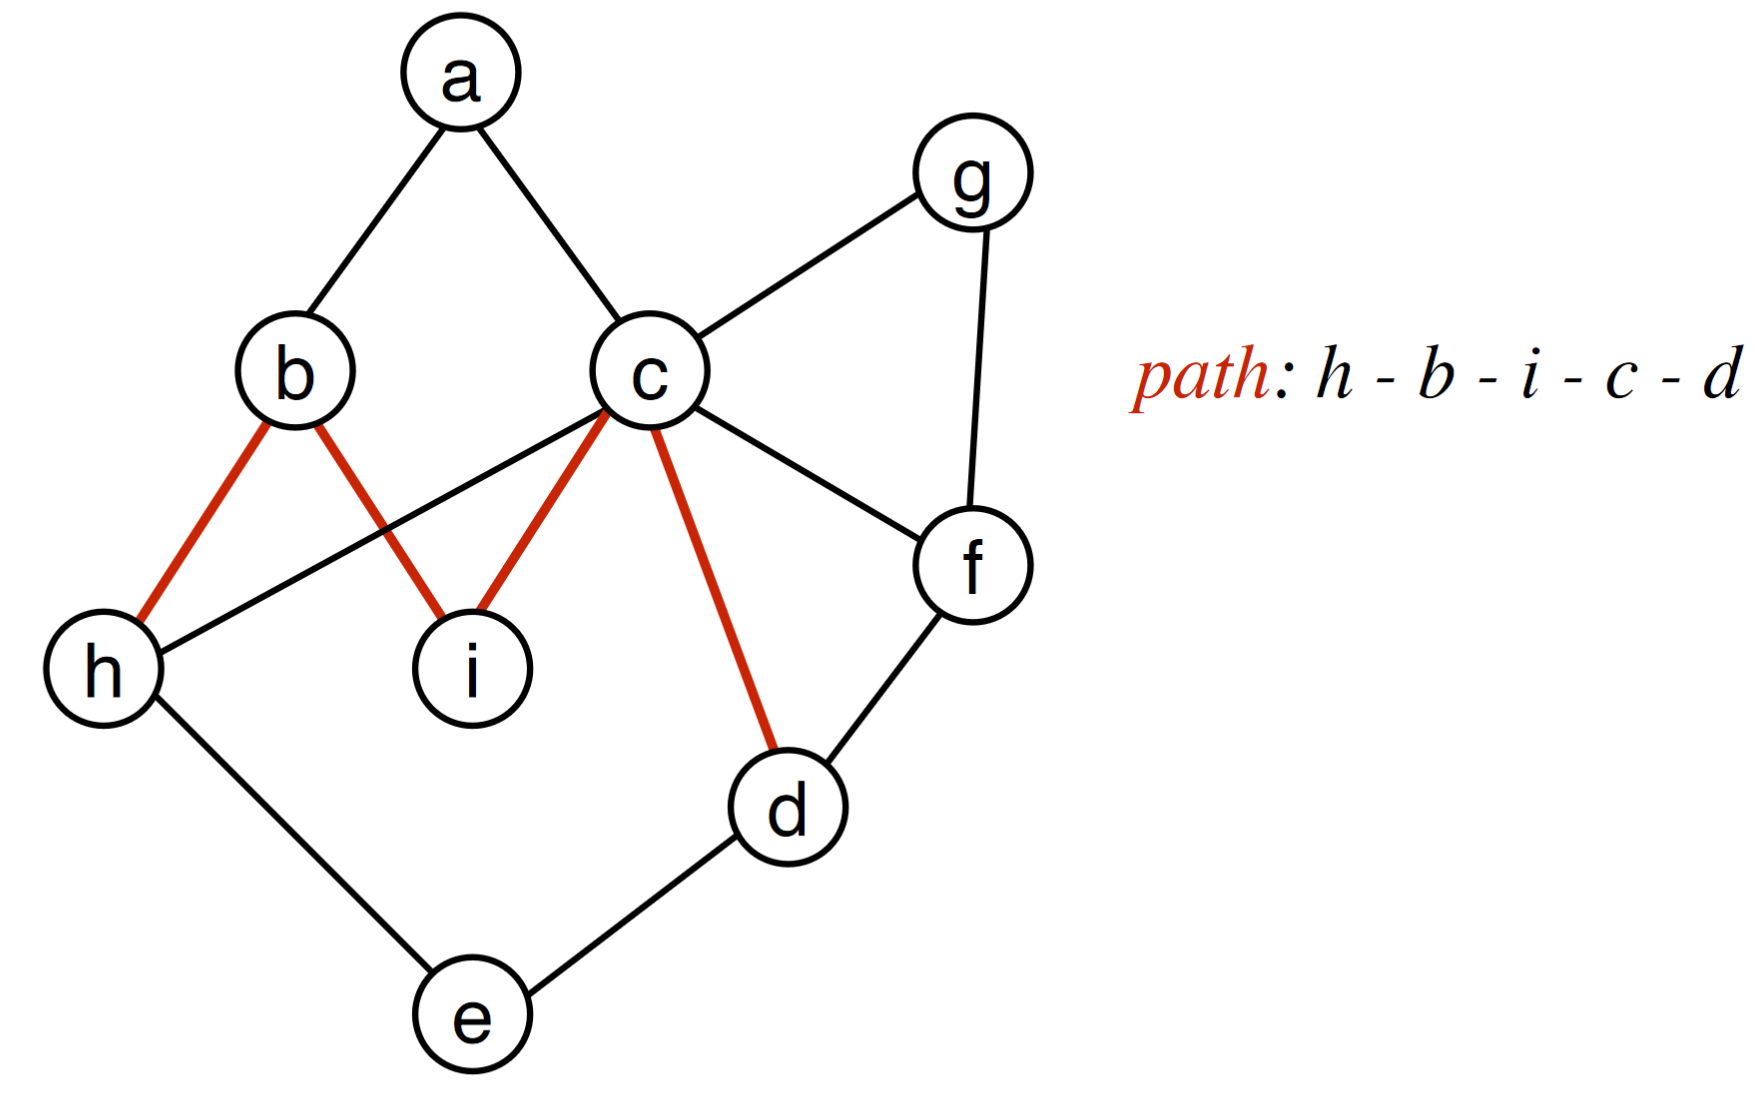
\includegraphics[height=1.8in]{./Sections/graphs/path_graph.png}
    \end{center}
     \caption{A graph with a simple path from $h$ to $d$.}\label{fig:path_graph}
  \end{figure}

\begin{Def}[Connectivity]

    A graph is \textbf{connected} if there is a path between every pair of vertices.\\
    A graph is \textbf{disconnected} if there are two vertices with no path between them.\\
    \underline{Connected graphs of $n$ nodes have at least $n-1$ edges.}
\end{Def}
\begin{figure}[h]
    \begin{center}
      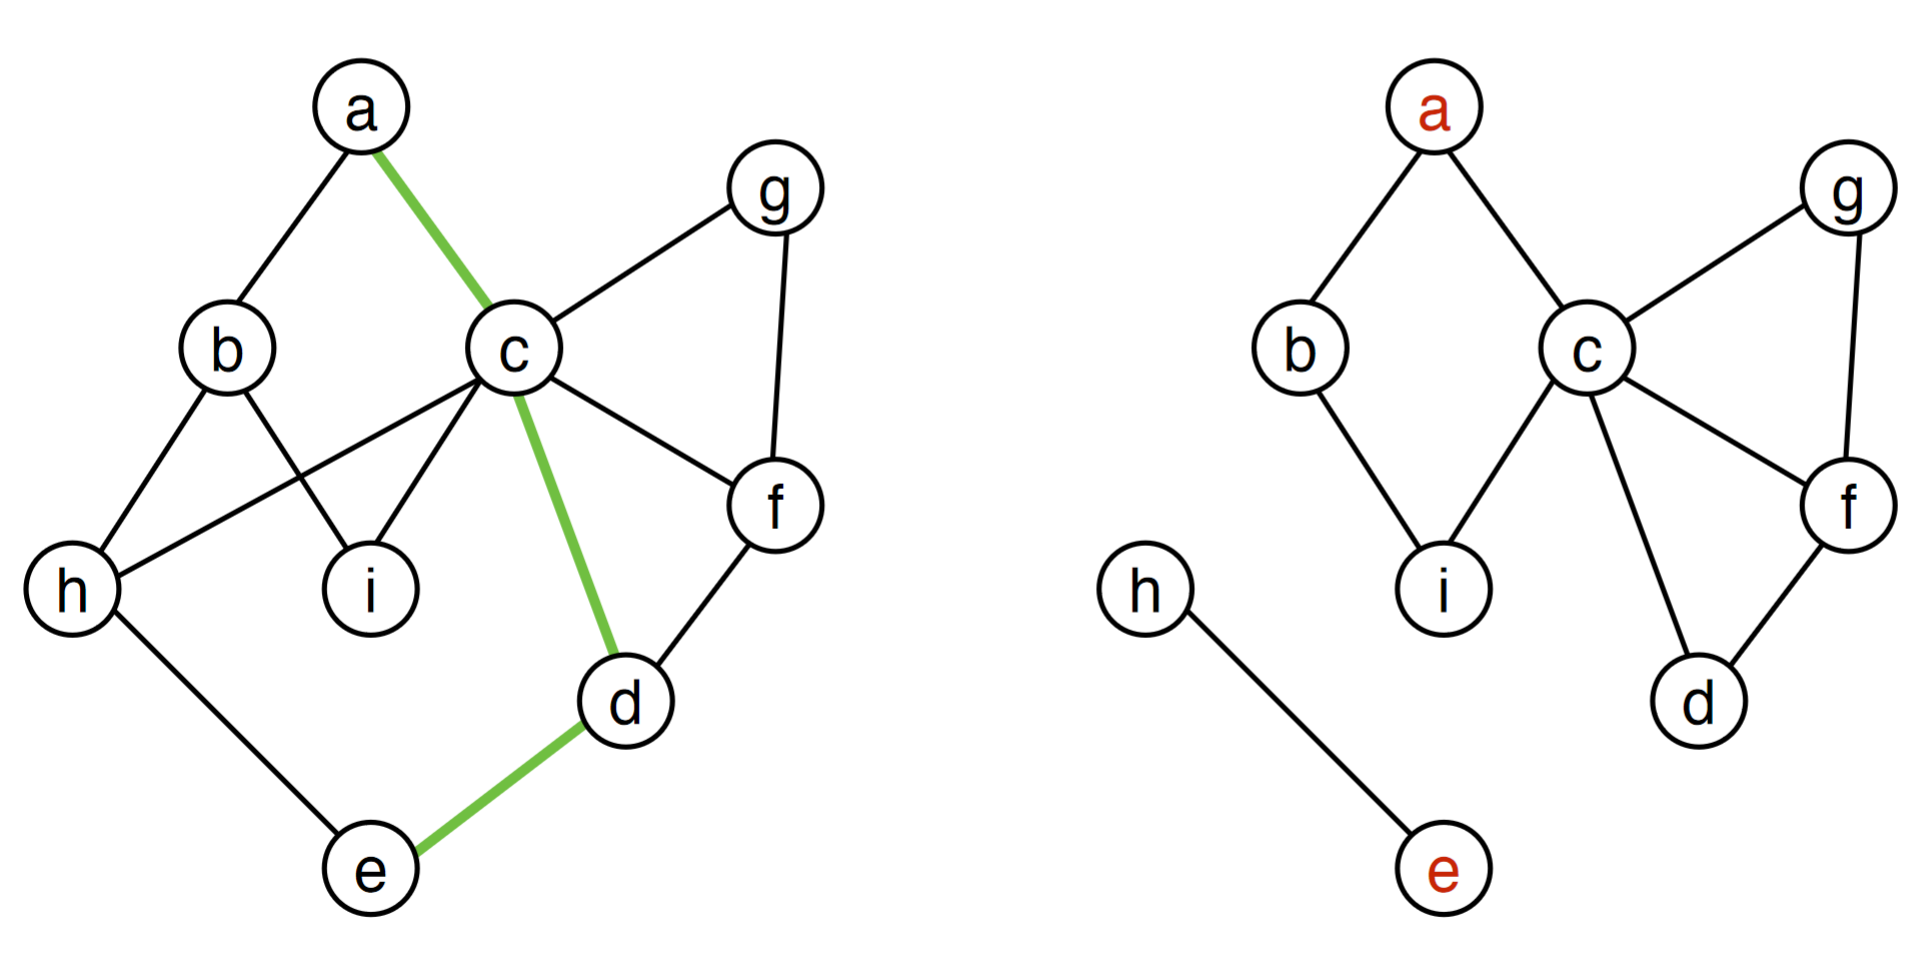
\includegraphics[height=1.8in]{./Sections/graphs/con_graph.png}
    \end{center}
     \caption{A connected graph $a\leftrightarrow c \leftrightarrow d \leftrightarrow e$  and disconnected graph.}\label{fig:con_graph}
  \end{figure}

  \newpage
  \begin{Def}[Adjacency Matrix]
      
      An \textbf{adjacency matrix} is an $n\times n$ matrix where such that $A[i][j] = 1$ if there is an edge between nodes $i$ and $j$.

  \end{Def}

  
\begin{figure}[h]
  \begin{center}
    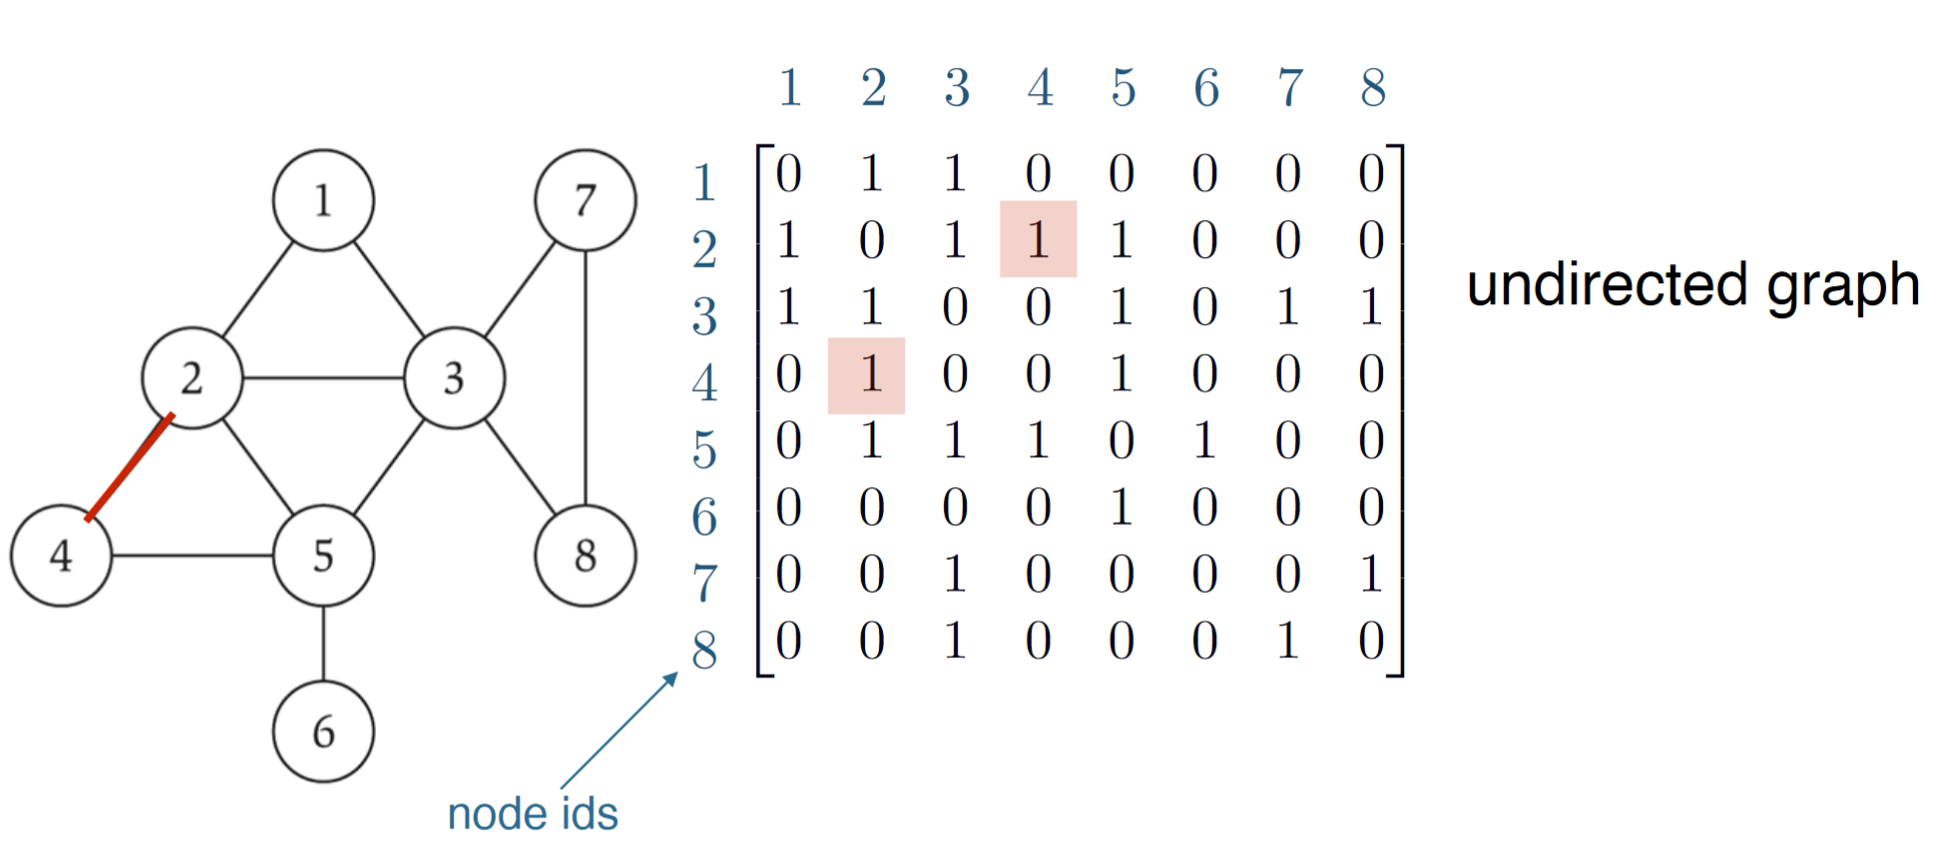
\includegraphics[height=1.5in]{./Sections/graphs/adj_matrix.png}
  \end{center}
   \caption{An adjacency matrix where the path $4\leftrightarrow2$ is highlighted ($A[2][4]$ or $A[4][2]$)}\label{fig:adj_matrix}
\end{figure}
\begin{theo}[Properties of Adjacency Matrix]

  The following properties hold for adjacency matrices:
    \begin{itemize}
        \item An undirected graph is symmetric about the diagonal.
        \item A directed graph is not symmetric about.
        \item A weighted graph has the weight of the edge instead of binary.
    \end{itemize}
    \noindent
    \textbf{Space Complexity:} $\Theta (n^2)$; \textbf{Time Complexities:}\\
    \textbf{Index edge $A[i][j]$:} $\Theta (1)$; \textbf{List neighbors $A[i]$}: $\Theta(n)$; \textbf{List all edges:} $\Theta(n^2)$.
\end{theo}

\begin{figure}[h]
  \begin{center}
    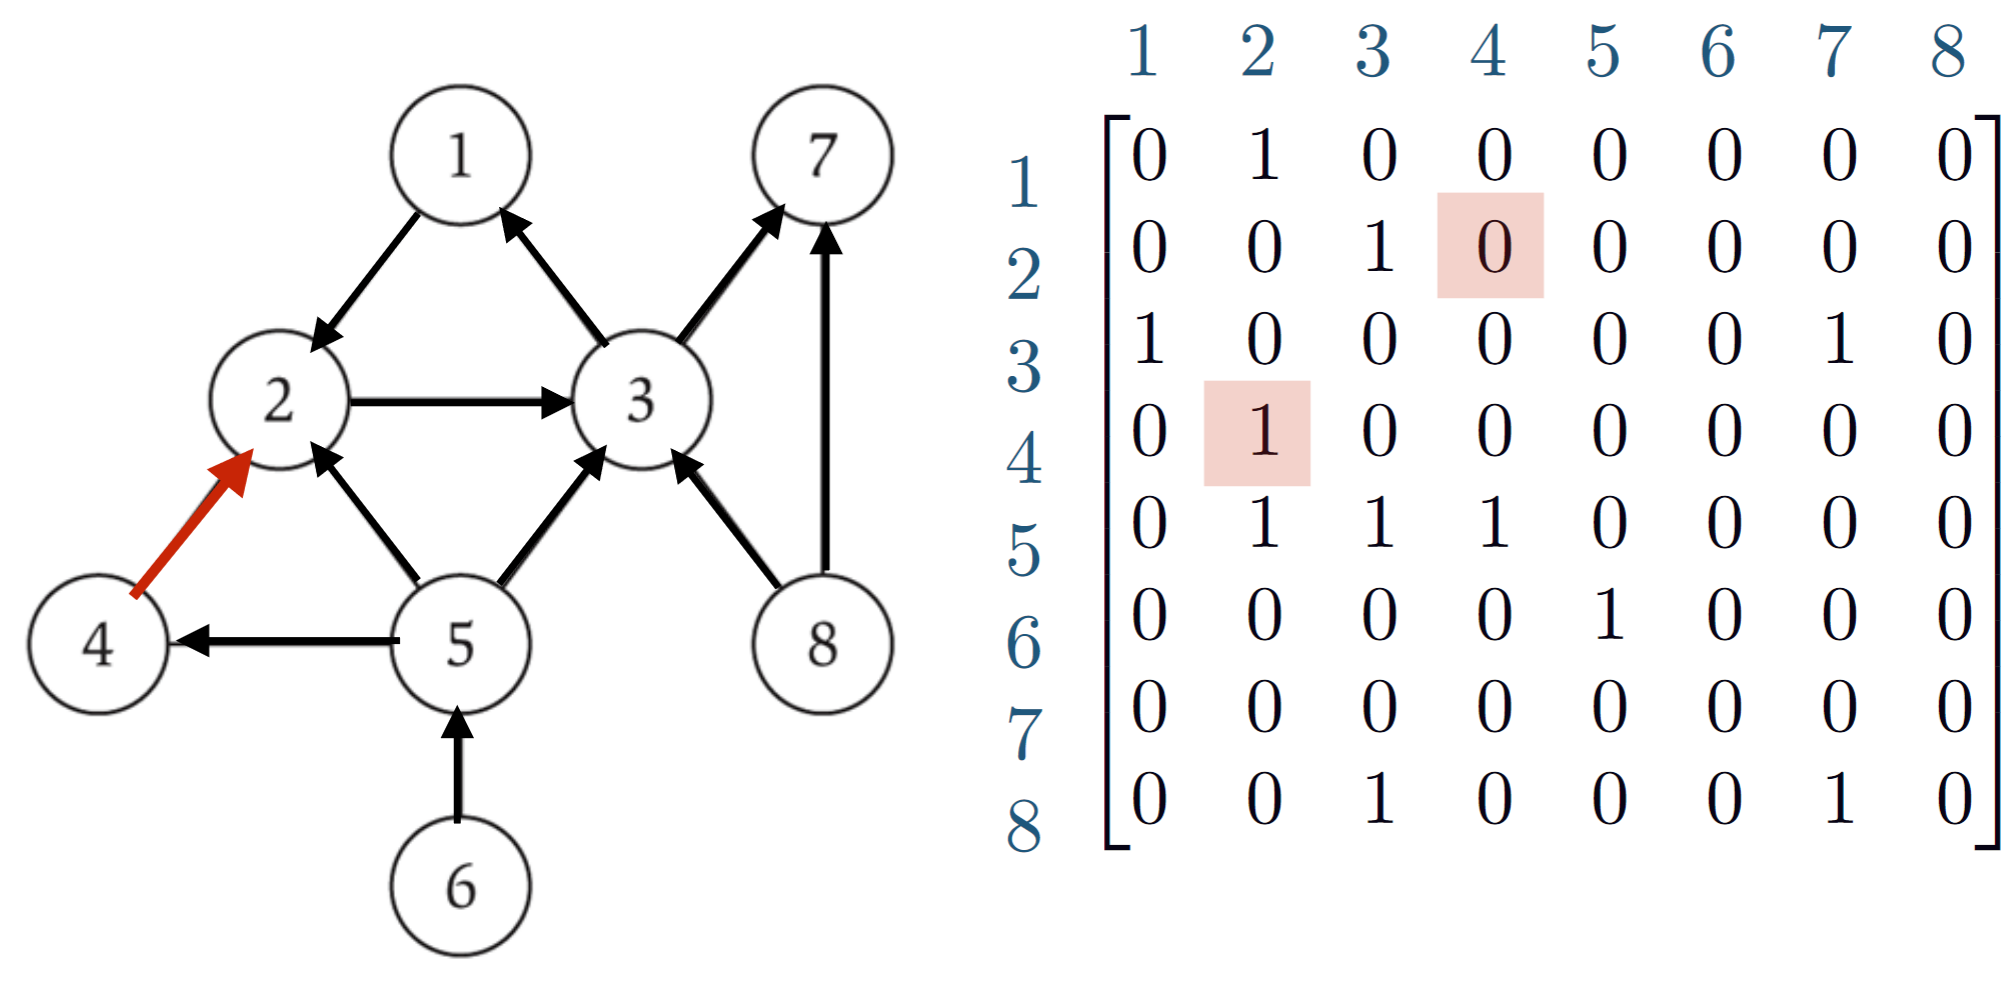
\includegraphics[height=1.5in]{./Sections/graphs/adj_matrix_dir.png}
  \end{center}
   \caption{An adjacency matrix of a directed graph with path $4\rightarrow2$ highlighted.}\label{fig:adj_matri_dir}
\end{figure}

\newpage
\begin{Def}[Adjacency List]

  \label{def:adj_list}
    An \textbf{adjacency list} is a list of keys where each key has a list of neighbors; This often takes the form of a hash-table:
    \textbf{Space Complexity:} $\Theta (n+m)$ for $n$ nodes and $m$ total edges; \textbf{Time Complexities:}
    \textbf{Index key:} $\Theta (1)$; \textbf{List key neighbors:} $\Theta(\text{\# of outdegrees})$; \textbf{List all edges:} $\Theta(n+m)$;
    \textbf{Insert edge:} $\Theta(1)$. \textbf{Note:} $m\leq n^2$ (all nodes connected to all nodes), though typically 
    in practice, $m < n$.
\end{Def}

\begin{figure}[h]
  \begin{center}
    \includegraphics[height=1.5in]{./Sections/graphs/adj_list.png}
  \end{center}
   \caption{An adjacency list of a directed graph, notably $c$ has no outdegrees.}\label{fig:adj_list}
\end{figure}







% \vspace{-1em}
\section{Breath-First and Depth-First Search}
\subsection{High-Level Overview}
Two general methods for traversing a graph are, \textbf{breadth-first search} and \textbf{depth-first search}.

\label{sec:bfs_dfs}
\begin{Def}[Cycle]

    A \textbf{cycle} is a path that starts and ends at the same node.
\end{Def}
\textbf{Example:} In the above Figure (\ref{fig:adj_matri_dir}), $1\rightarrow 2 \rightarrow 3 \rightarrow 1$ form a cycle.
\begin{Def}[Trees]

    A \textbf{tree} is a connected graph with no cycles. A \textbf{leaf-nodes} is the outer-most nodes of a tree. A \textbf{branch} is a path from the root to a leaf.
    \textbf{Interior nodes} have at least one child.  
\end{Def}

\begin{Tip}
Watch this entire section: \href{https://youtu.be/xHYS6IdpaDc?feature=shared}{BFS \& DFS (Edge Types, Traversal Orders, \& Code)}.
\end{Tip}
\newpage
\begin{theo}[Tree Identity]

    Let $G$ be an undirected graph of $n$ nodes. Then any two statements imply the third:
    \begin{center}

        \noindent
        (i.) $G$ is connected. \quad
        (ii.) $G$ has $n-1$ edges. \quad
        (iii.) $G$ has no cycles.
    \end{center}
\end{theo}

\begin{Def}[Rooted Trees]

        A tree \textbf{root} is a designated starting node, which all other nodes follow. The root has
        no parent/ancestors (proceeding node), and all other nodes are descendants (children).\\

        \noindent
        A \textbf{subtree} is a tree formed by picking another node as the root, representing a subset of 
        the original tree.
\end{Def}


\begin{Def}[Levels and Heights]

  The \textbf{level} (or \textbf{depth}) of a node $v$ in a tree is the number of edges on the path from the root to $v$, so $\mathrm{level}(\text{root})=0$.  
  The \textbf{height} of a node $v$ is the number of edges on the longest downward path from $v$ to any leaf.  
  The \textbf{height} of a tree is defined as the height of its root node.
\end{Def}

\begin{figure}[h]
    \begin{center}
      \includegraphics[height=2in]{./Sections/graphs/rooted_tree.png}
    \end{center}
     \caption{The right shows a rooted tree with root $s$, with $a$ and $b$ as direct children. A possible
     subtree starts with node $b$, only consisting of $\{b, e,f,g\}$. \textbf{Note:} A tree is 
     not necessarily directed, while a rooted tree is (floods outwards from the root)}\label{fig:rooted_tree}
  \end{figure}



\newpage
\begin{Def}[Breadth-First Search (BFS)]

    In a \textbf{breadth-first search}, we start at a node's children first before moving onto their children's children in level order.
\end{Def}
\begin{figure}[h]
    \begin{center}
      \includegraphics[height=2in]{./Sections/graphs/bfs.png}
    \end{center}
     \caption{A BFS tree traversal preformed on a graph with each level enumerated}\label{fig:bfs}
  \end{figure}

\begin{theo}[Properties of BFS]
    
    BFS run on any graph $T$ produces a tree $T'$ with the following properties:
    \begin{enumerate}
        \item [(i.)] $T'$ is a tree.
        \item [(ii.)] $T'$ is a rooted tree with the starting node as the root.
        \item [(iii.)] The height of $T'$ is the shortest path from the root to any node.
        \item [(iv.)] Any sub-paths of $T'$ are also shortest paths.
    \end{enumerate}
\end{theo}
\begin{Proof}[Proof of BFS]

    (i.) and (ii.) follow from the definition of a tree. (iii.) and (iv.) follow that since a tree 
    contains a direct path to any given node in our parent child relationship, that path must be the shortest.
\end{Proof}
\begin{Tip}
    In a family tree, there is only one path from each ancestor to each descendant.
\end{Tip}

\newpage 

\noindent
We create a BFS algorithm from what we know, though not the best implementation:
\begin{Func}[BFS Algorithm - \texttt{BFS($s$)}]
    Breadth-First Search starting from node $s$.
    
    \vspace{.5em}
    \noindent
    \textbf{Input:} Graph $G = (V, E)$ and starting node $s$.\\
    \textbf{Output:} Levels of each vertex from $s$.\\
    \begin{algorithm}[H]
        \SetAlgoLined
        \SetKwProg{Fn}{Function}{:}{}
        \Fn{\texttt{BFS($s$)}}{
            \For{each $v \in V$}{
                Level[$v$] $\gets \infty$\;
            }
            Level[$s$] $\gets 0$\;
            Add $s$ to $Q$\;
            \While{$Q$ not empty}{
                $u \gets Q$.Dequeue()\;
                \For{each $v \in G[u]$}{
                    \If{Level[$v$] $= \infty$}{
                        Add edge $(u, v)$ to tree $T$ (parent[$v$] $= u$)\;
                        Add $v$ to $Q$\;
                        Level[$v$] $\gets$ Level[$u$] + 1\;
                    }
                }
            }
        }
    \end{algorithm}
\end{Func}
\vspace{-2em}
\begin{figure}[h]
    \begin{center}
      \includegraphics[height=2.9in]{./Sections/graphs/bfs_q.png}
    \end{center}
     \caption{A table showing the queue at each level of iteration}\label{fig:bfs_q}
  \end{figure}

  \newpage

We analyze the time and space complexity in the below Figure (\ref{fig:bfs_q_ana}):

\begin{figure}[h]
    \begin{center}
      \includegraphics[height=2in]{./Sections/graphs/bfs_q_ana.png}
    \end{center}
     \caption{An analysis showing $O(m+n)$ for both time and space complexity}\label{fig:bfs_q_ana}
  \end{figure}
  \begin{Proof}[Claim 1 for BFS]
    Let $s$ be the root of the BFS tree, then:
    \textbf{Proof:} Induction on the distance from $s$ to $u$.\\
    \textbf{Base case} ($u = s$): The code sets Level[$s$] = 0, and there is no path to find since the path has length 0.\\
    \textbf{Induction hypothesis:} For every node $u$ at distance $\leq i$, Claim 1 holds.\\
    \textbf{Induction step:}
    \begin{itemize}
        \item Let $v$ be a node at distance exactly $i + 1$ from $s$. Let $u$ be its parent in the BFS tree.
        \item The code sets Level[$v$] = Level[$u$] + 1.
        \item Let $x$ be the last node before $v$ on a shortest path from $s$ to $v$. Since $v$ is at distance $i + 1$, then $x$ must be at distance $i$, and so Level[$x$] = $i$ (by induction hypothesis).
        \item If $u = x$, we are done!
        \item If $u \neq x$, then it must be that $u$ was explored before $x$, since otherwise $x$ would be the parent of $u$.
        \item Since we explore nodes in order of level, Level[$u$] $\leq$ Level[$x$] = $i$.
        \item If Level[$u$] = $i$, then we are done.
        \item If Level[$u$] $<$ $i$, then the path $s \sim u \to v$ has length at most $i$, which contradicts the assumption that the distance of $v$ is $i + 1$.
    \end{itemize}
    
    \noindent
    We conclude that Level[$u$] = $i$, Level[$v$] = $i + 1$, and the path in the BFS tree that goes from $s$ to $u$ to $v$ has length $i + 1$.
    \end{Proof}
    
    \newpage
    \begin{Def}[Depth-First Search (DFS)]

        In a \textbf{depth-first search}, we recursively explore each an entire branch before moving onto the next.
    \end{Def}

    \begin{Func}[DFS Algorithm - \texttt{DFS($G$)}]
        Depth-First Search on graph $G$ (recursive).
    
        \vspace{.5em}
        \noindent
        \textbf{Input:} Graph $G = (V, E)$.\\
        \textbf{Output:} Discovery and finishing times for each vertex.
        
        \begin{algorithm}[H]
            \SetAlgoLined
            \SetKwProg{Fn}{Function}{:}{}
            \Fn{\texttt{DFS($G$)}}{
                \For{each $u \in G$}{
                    $u$.state $\gets$ \texttt{unvisited}\;
                }
                time $\gets 0$\;
                \For{each $u \in G$}{
                    \If{$u$.state == \texttt{unvisited}}{
                        \texttt{DFS-Visit($u$)}\;
                    }
                }
            }
            \vspace{.5em}
            \Fn{\texttt{DFS-Visit($u$)}}{
                time $\gets$ time + 1\;
                $u.d \gets$ time \; // record discovery time\;
                $u$.state $\gets$ \texttt{discovered}\;
                \For{each $v \in G[u]$}{
                    \If{$v$.state == \texttt{unvisited}}{
                        \texttt{DFS-Visit($v$)}\;
                    }
                }
                $u$.state $\gets$ \texttt{finished}\;
                time $\gets$ time + 1\;
                $u.f \gets$ time\; // record finishing time\;
            }
        \end{algorithm}

        \noindent
        \textbf{Time and Space Complexity:} $O(n+m)$ where $n$ is the number of vertices and $m$ the number of edges.
    \end{Func}

    \newpage

    \begin{Proof}[DFS Correctness]

        \textbf{Case 1:} When $s$ is discovered, there is a path of unvisited vertices from $s$ to $y$. We use induction on the length $L$ of the unvisited path from $x$ to $y$.
        \begin{itemize}
            \item \textbf{Base case:} There is an edge $(x, y)$, and $y$ is unvisited.
            \item \textbf{Induction hypothesis:} Assume that the claim is true for all nodes reachable via $k$ unvisited nodes.
            \item \textbf{Induction step:}
            \begin{itemize}
                \item Consider $u$ reachable via $k + 1$ unvisited nodes.
                \item Let $z$ be the last node on the path before $y$, and $z$ is discovered from $x$ (by I.H.).
                \item The edge $(z, y)$ will be explored from $x$, ensuring that $y$ is eventually visited.
            \end{itemize}
        \end{itemize}
        \noindent
        Thus, DFS-Visit($x$) explores all nodes reachable from $x$ through a path of unvisited nodes, as required.
        \end{Proof}

% \begin{figure}[h]
%     \begin{center}
%       \includegraphics[height=3.5in]{./Sections/graphs/dfs.png}
%     \end{center}
%      \caption{A graph showing our $d$ discovered and $f$ finished times, denoted in pairs $(f,d)$.}\label{fig:dfs}
%   \end{figure}
    
\subsection{Edge Classifications -- Directed Graphs}

\noindent
To build our intuition around edge classifications, we'll follow a walkthrough of DFS \& BFS on directed graphs
to build our intuition. We'll follow the below format:

\begin{figure}[h]
    \begin{center}
    \includegraphics[width=1\textwidth]{./Sections/graphs/edges/eg_1.png}
    \end{center}
     \caption{A table for start and finish times of each visited nodes, our stack to keep track of traversals, the graph that shall be traversed, and a timer for DFS (BFS will use a queue).}
     \label{fig:edge_class}
  \end{figure}

\newpage 

\noindent
Let's start by filling out a partial DFS traversal:

\begin{figure}[h]
    \begin{center}
    \includegraphics[width=1\textwidth]{./Sections/graphs/edges/eg_2.png}
    \end{center}
     \caption{So far we have asked $s$ to put all their children on the stack at timestamp 0. We 
     first investigate the first child $a$'s branch at time 1. It gives us $b$, for which we time stamp (2,3) for start and finish. We highlight the first the alternative $b$ branch in blue for distinction.
     The edges that are in our (start, finish) table are \underline{\textbf{Tree Edges}}.}
     \label{fig:edge_class_2}
  \end{figure}
\noindent

\begin{Def}[Forward Edge]

    A \textbf{non-tree edge} that connects an already discovered node to a descendant in the DFS tree is called a \textbf{forward edge}.
    Concretely, $(u, v)$ is a forward edge if given $u(s_1,f_1)$ and $v(s_2,f_2)$ of node id and a start finish time tuple, we have: $s_1 < s_2 < f_2 < f_1$.\\
    Where the \underline{\textbf{start time} of $u$ is less than $v$}, and the \underline{\textbf{finish time} of $u$ is greater than $v$}.
\end{Def}

\begin{figure}[h]
    \begin{center}
    \includegraphics[width=1\textwidth]{./Sections/graphs/edges/eg_3.png}
    \end{center}
     \caption{Continuing from Figure (\ref{fig:edge_class_2}), $b$ and $a$ are taken off the stack. The next $b$ on the stack is a \textbf{forward edge}, as $s$ has a 
     smaller start time, and a foreseeable finish time than the table's $b$.}
     \label{fig:edge_class_3}
  \end{figure}

\newpage 

\noindent
The next two are \textbf{cross and back edges}:

\begin{Def}[Cross Edge]

    A \textbf{non-tree edge} that connects branches of a tree is called a \textbf{cross edge}.
    In particular, $(u, v)$ is a cross edge if $v$ is not a descendant or ancestor of $u$.
    Concretely, given $u(s_1,f_1)$ and $v(s_2,f_2)$ of node id and a start finish time tuple, we have: $s_2 < s_1 < f_2 < f_1$.\\
    Where the \underline{\textbf{start and finish time} of $u$ is greater than $v$}.
\end{Def}

\begin{Def}[Back Edge]

    A \textbf{non-tree edge} that connects a node to an ancestor in the tree is called a \textbf{back edge}.
    Concretely, given $u(s_1,f_1)$ and $v(s_2,f_2)$ of node id and a start finish time tuple, we have: $s_2 < s_1 < f_1 < f_2$.\\
    Where the \underline{\textbf{start time} of $u$ is greater than $v$}, but the \underline{\textbf{finish time} of is less than $v$}.
\end{Def}

\begin{figure}[h]
    \begin{center}
    \includegraphics[width=1\textwidth]{./Sections/graphs/edges/eg_4.png}
    \end{center}
     \caption{Continuing from Figure (\ref{fig:edge_class_3}), $b$ and $a$ are taken off the stack. 
     Next on the stack is $c$, which reveals children $b$ and $s$; Here, $b$ has already been processed (cross edge), and 
     $s$ discovered, but yet to be finished (back edge). There is nothing else to explore, so we finish $c$.
     \textbf{Note:} There is no classifications for self referential edges.}
     \label{fig:edge_class_4}
  \end{figure}

\noindent
Next we'll see how our classifications work on BFS.

\newpage 

\noindent
Starting with the same graph as before we instead run BFS:

\begin{figure}[h]
    \begin{center}
    \includegraphics[width=1\textwidth]{./Sections/graphs/edges/eg_5.png}
    \end{center}
     \caption{We start with $s$ modeling the queue history on the left. The first graph is our original graph finished, and on the right it is 
     redrawn for clarity.}
     \label{fig:edge_class_5}
  \end{figure}

\begin{theo}[DFS \& BFS Directed Graphs]
    
    Between DFS and BFS, the following holds:
    \begin{itemize}
        \item \textbf{DFS}: Tree, back, forward, and cross edges (all edges).
        \item \textbf{BFS}: Tree, cross, and back edges (no forward edges).
    \end{itemize}
\end{theo}

\noindent
Additionally, one may find the following theorem helpful:
\begin{theo}[DFS and Cycles]

    Let DFS run on graph $G$, then:
    \[
\left( G \text{ has a cycle} \right) \iff \left( \text{DFS run reveals \textcolor{red}{back edges}} \right)
\]

  \end{theo}
  \begin{Proof}[Proof of Cycles and Back Edges]
    \textbf{Proving} $\left( G \text{ has a cycle} \right) \Longleftarrow \left( \text{DFS run reveals \textcolor{red}{back edges}} \right)$: Every back edge creates a cycle.\\
    \textbf{Proving} $\left( G \text{ has a cycle} \right) \Longrightarrow \left( \text{DFS run reveals \textcolor{red}{back edges}} \right)$ Suppose $G$ has a cycle:
    Let $u_1$ be the first discovered vertex in the cycle, and let $u_k$ be its predecessor in the cycle.
    $u_k$ will be discovered while exploring $u_1$.
    The edge $(u_k, u_1)$ will be a back edge.
    \end{Proof}

\newpage 

\noindent
Next we deal with undirected graphs briefly and give a summary:
\begin{figure}[h]
    \begin{center}
    \includegraphics[width=1\textwidth]{./Sections/graphs/edges/eg_6.png}
    \end{center}
     \caption{Here DFS and BFS are shown, with the original graph on the far right. Here it's quite peculiar to have a double-edge
     in an undirected graph. In our case it's redundant and may be counted as a single edge.}
     \label{fig:edge_class_6}
  \end{figure}

  \noindent
\textbf{Summary:}\\
\noindent
This allows us to summarize the edge classifications for both directed and undirected graphs in the below table:
\begin{table}[h]
    \centering
    \begin{tabular}{|c|c|c|}
        \hline
        \textbf{Graph Type} & \textbf{DFS Edge Types} & \textbf{BFS Edge Types} \\ \hline
        Directed Graphs & Tree, Back, Forward, Cross & Tree, Back, Cross \\ \hline
        Undirected Graphs & Tree, Back & Tree, Cross \\ \hline
    \end{tabular}
    \caption{Edge classifications for DFS and BFS in directed and undirected graphs.}
    \label{tab:edge_classifications}
\end{table}

\begin{table}[h]
    \centering
    \begin{tabular}{|c|c|c|}
        \hline
        \textbf{Edge Type} & \textbf{Start Condition} & \textbf{Finish Condition} \\ \hline
        Forward Edge & less & greater \\ \hline
        Cross Edge & greater & greater \\ \hline
        Back Edge & greater & less \\ \hline
    \end{tabular}
    \caption{Summary of start and finish conditions for edge types by comparing the starting node 
    with its endpoint. E.g., in a forward edge $(u, v)$, the start time of $u$ is less than $v$, but the finish time is greater.}
    \label{tab:edge_timestamps}
\end{table}

\newpage 
% \section{Tree Types \& Traversals}

\subsection{Binary Trees: 2 Children}

\noindent
First we'll define a basic binary tree and then all its extensions.
\begin{Def}[Binary Tree]

    A \textbf{binary tree} is a tree where each parent node has at most two children.
\end{Def}

\begin{figure}[h]
    \begin{center}
    \includegraphics[width=\textwidth]{./Sections/graphs/binary_tree.png}
    \end{center}
     \caption{These are three examples of binary trees, including a single node (3).}\label{fig:binary_tree}
  \end{figure}

\noindent
To simply do a binary tree traversal, we may employ the following methods:
\begin{Func}[DFS Binary Tree Traversal - \texttt{DFS($T$)}]
    Depth-First Search on binary tree $T$ (recursive).
    
    \vspace{.5em}
    \noindent
    \textbf{Input:} Binary tree $T$.\\
    \textbf{Output:} Nodes in pre-order, in-order, and post-order.
    
    \begin{algorithm}[H]
        \SetAlgoLined
        \SetKwProg{Fn}{Function}{:}{}
        \Fn{\texttt{DFS($T$)}}{
            \If{$T$ is not empty}{
                Visit node $T$\;
                \texttt{DFS($T.left$)}\;
                \texttt{DFS($T.right$)}\;
            }
        }
    \end{algorithm}
    \noindent
    \rule{\textwidth}{0.4pt}
    \textbf{Time Complexity:} Given n nodes, and a force of a tree format, we have $n-1$ edges. Therefore with $m$ edges, $n+m = n+(n-1)$, hence $O(n)$ time.\\
    \textbf{Space Complexity:} again, we have $O(n)$ space for the stack.
\end{Func}

\noindent
$\mathbf{\rightarrow}$ \textbf{\underline{BFS has the same complexities} as per the same reasoning as the above function.}\\

\newpage
\noindent
The order in the above function is called \textbf{pre-order traversal};

\begin{Def}[Order Traversals]

    The order of traversal refers to the order in which nodes are visited/processed:
    \begin{itemize}
        \item \textbf{Pre-order:} Visit the node, then left, then right.
        \item \textbf{In-order:} Visit left, then the node, then right.
        \item \textbf{Post-order:} Visit left, then right, then the node.
    \end{itemize}
    In particular, \underline{\textbf{in-order traversal} is simply a run of \textbf{BFS}} as it processes the tree level by level starting 
    from the root.
\end{Def}

\noindent
Below is an example of all three:

\begin{Example}[Binary Tree Traversals (Part 1)]

    \begin{lstlisting}[language=Python, numbers=none]
    # Pre-order Traversal
    def PreOrder(T):
        if T is not None:
            visit(T)
            PreOrder(T.left)
            PreOrder(T.right)

    # In-order Traversal
    def InOrder(T):
        if T is not None:
            InOrder(T.left)
            visit(T)
            InOrder(T.right)

    # Post-order Traversal
    def PostOrder(T):
        if T is not None:
            PostOrder(T.left)
            PostOrder(T.right)
            visit(T)

    # Level-order Traversal
    def LevelOrder(T):
        BFS(T)
    \end{lstlisting}
\end{Example}

\newpage

\noindent
Now to show how this actually looks:
\begin{figure}[h]


    \hspace {-10em} \includegraphics[width=1.5\textwidth]{./Sections/graphs/binary_tree_traversals.png}
  
     \caption{%
        The above binary tree has the following traversals:\\[1em]
           $\bullet$\quad  \textbf{Pre-order:}  \hspace{.5em} G, E, C, D, A, H, K, F, M\\
           $\bullet$\quad  \textbf{In-order:}   \hspace{1.2em} C, E, A, D, G, H, F, K, M\\
           $\bullet$\quad  \textbf{Post-order:} \hspace{.05em} C, A, D, E, F, M, K, H, G\\
           $\bullet$\quad \textbf{Level-order:} G, E, H, C, D, K, A, F, M\\[1em]
         Notably, if there is no left or right child to explore for that particular traversal order, that node then and there is processed.
     For example, in in-order traversal, since $C$ has no left child, it is processed first. The same goes for Post-order, where $D$ has no right child, so it is processed.
     }\label{fig:binary_tree_traversals}
  \end{figure}

\begin{Def}[Types of Binary Trees]

    There are several types of binary trees, each with its own properties:
    \begin{itemize}
        \item \textbf{Full Binary Tree:} Every node has either 0 or 2 children.
        \item \textbf{Complete Binary Tree:} All levels are fully filled except possibly the last level, which is filled from left to right.
        \item \textbf{Perfect Binary Tree:} All interior nodes have two children and all leaves are at the same level.
        \item \textbf{Balanced Binary Tree:} The height of the left and right subtrees of every node differ by at most one.
    \end{itemize}
    \noindent
    \textbf{Note:} A full binary tree is not necessarily complete, and a complete binary tree is not necessarily full.
\end{Def}

\newpage

\noindent
Observe the following examples of binary trees:
\begin{figure}[h]
    \begin{center}
    \includegraphics[width=\textwidth]{./Sections/graphs/search/binary_tree_types.png}
    \end{center}
     \caption{These are examples of different types of binary trees (BT).}\label{fig:binary_tree_types}
  \end{figure}


\subsection{Binary Search Tree}
\noindent
A binary search tree is a stricter form of a binary tree, which gives us an efficient search algorithm.
\begin{Def}[Binary Search Tree (BST) -- Overview]

    \label{def:binary_search_tree}

    A \textbf{binary search tree} is a binary tree where:
    
    \begin{center}
        left child $<$ parent node $\leq$ right child
    \end{center}
    \noindent
    \textbf{Note:} A Binary Tree \underline{\textbf{is not}} a Binary Search Tree, unless it satisfies the above conditions.
\end{Def}

\begin{figure}[h]
    \begin{center}
    \includegraphics[width=\textwidth]{./Sections/graphs/search/bst.png}
    \end{center}
     \caption{Visual Representation of Definition (\ref{def:binary_search_tree}), where $k$ is 
     the parent node with its respective left (less than) and right (greater than or equal to) nodes.}\label{fig:binary_search_tree}
  \end{figure}

\noindent
The next few pages we discuss \textbf{Searching, Insertion, and Deletion} in a binary search tree.
  
\newpage
\begin{Func}[Binary Search Tree (BST) -- Searching]

    Given a BST root node $T$ and a desired value $v$, we can search for $v$ in $T$ as follows:
  \newpage 
    \vspace{.5em}
    \noindent
    \textbf{Input:} BST root node $T$, value $v$.\\
    \textbf{Output:} Node containing $v$ or null if not found.
    
    \begin{algorithm}[H]
        \SetAlgoLined
        \SetKwProg{Fn}{Function}{:}{}
        \Fn{\texttt{Search($T, v$)}}{
            \While{$T$ is not null}{
                \If{$T.value = v$}{
                    \KwRet{$T$}\;
                }
                \If{$v < T.value$}{
                    $T \gets T.left$\;
                }
                \Else{
                    $T \gets T.right$\;
                }
            }
            \KwRet{null}\;
        }
    \end{algorithm}
    \noindent
    \rule{\textwidth}{0.4pt}
    \textbf{Time Complexity:} $O(h)$ where $h$ is the height of the tree. In a balanced BST, this is $O(\log n)$, but in the worst case (unbalanced), it can be $O(n)$.
\end{Func}

\begin{figure}[ht!]
    \begin{center}
    \includegraphics[width=\textwidth]{./Sections/graphs/search/bst_search.png}
    \end{center}
     \caption{Searching for a value in a binary search tree. The worst case is a noodle (all right nodes), forcing $n$ traversals, i.e., the height (within a constant). One could imagine these nodes as complex objects, where the value $v$ is a key, and the node itself contains more data.}\label{fig:bst_search}
  \end{figure}

\begin{theo}[Property of Binary Search Trees]

    \label{theo:bst_property}

    In a binary search tree, for any node $N$:
    \begin{itemize}
        \item All values in the left subtree of $N$ are less than the value of $N$.
        \item All values in the right subtree of $N$ are greater than or equal to the value of $N$.
    \end{itemize}
\end{theo}

\newpage 
\noindent
Insertion is the same an searching, except we insert upon reaching a null node.
\begin{Func}[Binary Search Tree (BST) -- Insertion]

    Given a BST root node $T$ and a value $v$, we can insert $v$ into $T$ as follows:
    
    \vspace{.5em}
    \noindent
    \textbf{Input:} BST root node $T$, value $v$.\\
    \textbf{Output:} Updated binary search tree with $v$ inserted.
    
    \begin{algorithm}[H]
        \SetAlgoLined
        \SetKwProg{Fn}{Function}{:}{}
        \Fn{\texttt{Insert($T, v$)}}{
            $parent \gets$ null; $current \gets T$\;
            \While{$current$ is not null}{
                $parent \gets current$\;
                \If{$v < current.value$}{
                    $current \gets current.left$\;
                }
                \Else{
                    $current \gets current.right$\;
                }
            }
            \vspace{1em}
            \tcp{After the while loop terminates}
            \If{$parent$ is null}{
                \KwRet{$v$} \tcp*[l]{Tree was empty, $v$ becomes root}
            }
            \If{$v < parent.value$}{
                $parent.left \gets v$\;
            }
            \Else{
                $parent.right \gets v$\;
            }
            \KwRet{$T$}\;
        }
    \end{algorithm}
    \noindent
    \rule{\textwidth}{0.4pt}
    \textbf{Time Complexity:} $O(h)$ where $h$ is the height of the tree. In a balanced BST, this is $O(\log n)$, but in the worst case (unbalanced), it can be $O(n)$.\\
\end{Func}

\noindent
Deletion is a bit more complex, as we have to consider removing intermediate nodes:

\begin{theo}[Binary Search Tree (BST) -- Deletion]

    When deleting a node from a binary search tree, we must consider three cases:
    \begin{itemize}
        \item \textbf{$v$ has no children:} Remove the parent's reference to $v$.
        \item \textbf{$v$ has one child:} Replace the parent's reference to $v$'s child.
        \item \textbf{$v$ has two children:} Replace the parent's reference to $v$ with either:
            \begin{itemize}
                \item The \textbf{L}argest value in $v$'s \textbf{L}eft subtree (in-order predecessor).
                \item The \textbf{R}unt (smallest) value in $v$'s \textbf{R}ight subtree (in-order successor).
            \end{itemize}
    \end{itemize}

    \noindent
    This ensures that the binary search tree properties are maintained after deletion.
\end{theo}

\newpage
\begin{Func}[Binary Search Tree (BST) -- Deletion]

    Given a BST root node $T$ and a value $v$, we can delete $v$ from $T$ as follows:
    
    \vspace{.5em}
    \noindent
    \textbf{Input:} BST root node $T$, value $v$.\\
    \textbf{Output:} Updated binary search tree with $v$ deleted.
    
    \begin{algorithm}[H]
        \SetAlgoLined
        \SetKwProg{Fn}{Function}{:}{}
        \Fn{\texttt{Delete($T, v$)}}{
            $parent \gets$ null; $current \gets T$\;
            \While{$current$ is not null \textbf{and} $current.value \neq v$}{
                $parent \gets current$\;
                \If{$v < current.value$}{
                    $current \gets current.left$\;
                }
                \Else{
                    $current \gets current.right$\;
                }
            }
            \If{$current$ is null}{
                \KwRet{$T$} \tcp*[l]{Value not found}
            }
            \tcp{Case 1: Node has at most one child}
            \If{$current.left$ is null \textbf{or} $current.right$ is null}{
                \If{$current.left$ is not null}{
                    $child \gets current.left$\;
                }
                \Else{
                    $child \gets current.right$\;
                }
                \If{$parent$ is null}{
                    \KwRet{$child$} \tcp*[l]{Deleted root}
                }
                \If{$parent.left = current$}{
                    $parent.left \gets child$\;
                }
                \Else{
                    $parent.right \gets child$\;
                }
                \KwRet{$T$}\;
            }
            \tcp{Case 2: Node has two children}
            $succParent \gets current$\;
            $succ \gets current.right$ \tcp*[l]{Runt of Right subtree}
            \While{$succ.left$ is not null}{
                $succParent \gets succ$\;
                $succ \gets succ.left$\;
            }
            $current.value \gets succ.value$\;
            \If{$succParent.left = succ$}{
                $succParent.left \gets succ.right$\;
            }
            \Else{
                $succParent.right \gets succ.right$\;
            }
            \KwRet{$T$}\;
        }
    \end{algorithm}
    \noindent
    \rule{\textwidth}{0.4pt}
    \textbf{Time Complexity:} $O(h)$ where $h$ is the height of the tree. In a balanced BST, this is $O(\log n)$, but in the worst case (unbalanced), it can be $O(n)$.
\end{Func}

\newpage 

\noindent
Consider an example as we build a binary search tree and performing the above operations:
\begin{figure}[h]
    \centering
    \includegraphics[width=\textwidth]{./Sections/graphs/search/bst_ex.png}
    \caption{%
        \textbf{Note:} We use the Largest Left child (in-order predecessor) to replace the 2-children case. From 
        1--9 we insert values. From 10--11 we delete. In (10) we delete 8 (1-child case), we replace its 
        parent's reference to 8 with its only child 6. In (11) we delete 3 (2-children case), we replace its parent's reference to 3 with the largest left child, which is 2.
        One could imagine the in-order successor (smallest right child) would have 4 instead of 2, with 2 and 1 on its left subtree.}
    \label{fig:bst_operations}
\end{figure}

\newpage
% \section{Directed-Acyclic Graphs \& Topological Ordering}
Graphs may represent a variety of relationships, such as dependencies between tasks or the flow of information. 

\begin{Def}[Directed-Acyclic Graph (DAG)]
    
    A \textbf{directed-acyclic graph} is a directed graph with no cycles.
\end{Def}

\begin{figure}[h]
    \begin{center}
      \includegraphics[height=1.5in]{./Sections/graphs/dag/dag.png}
    \end{center}
     \caption{A DAG depicted by getting dressed for winter.}\label{fig:dag}
\end{figure}

\noindent
For each node to be processed its \textbf{dependencies} or parents must be processed first.

\newpage
\begin{Def}[Topological Ordering]

    Given a graph, a \textbf{topological ordering} is a linear ordering of nodes such that for every edge $(u,v)$, $u$ comes before $v$.
\end{Def}

\begin{figure}[h]
    \begin{center}
      \includegraphics[height=1.5in]{./Sections/graphs/dag/top.png}
    \end{center}
     \caption{A topological ordering of the DAG in Figure (\ref{fig:dag}) enumerated in red.}\label{fig:top}
\end{figure}
\noindent
Another possible ordering of $[1,2,3,4,5,6,7]$ is $[5, 6,1,2,3,4,7]$, as $5\rightarrow 6$ is independent.

\begin{theo}[Topological Sort]
    
    Given a DAG, a topological ordering can be found.
\end{theo}
\begin{figure}[h]
    \begin{center}
      \includegraphics[height=2.5in]{./Sections/graphs/dag/top_sort.png}
    \end{center}
     \caption{A topological sorting of a DAG $E$ and $v$ nodes}\label{fig:top_sort}
\end{figure}
\newpage
\begin{Proof}[Topological Sort via DFS]
    \textit{\textbf{Lemma:}} In a directed graph $G$, if (note necessarily acyclic):
    \begin{itemize}
        \item $(u, v)$ is an edge, and
        \item $v$ is not reachable from $u$,
    \end{itemize}
    Then in every run of DFS, $u.f > v.f$.
    
    \noindent
    \textit{\textbf{Proof:}}
    \begin{itemize}
        \item If $v$ is started before $u$, then the DFS-Visit($v$) will terminate without reaching $u$ (because there is no path to $u$).
        \item If $u$ is started before $v$, then the edge $(u, v)$ will be explored before $u$ is finished.
    \end{itemize}
    Therefore, in all cases, $u.f > v.f$.
\end{Proof}

\begin{Def}[Strongly Connected Components]

    A \textbf{strongly connected component} is a subgraph where every node is reachable from every other node. 
    Then we say $u\rightsquigarrow v$ and $v\rightsquigarrow u$ are \textbf{mutually reachable}. 
\end{Def}

\begin{figure}[h]
    \begin{center}
      \includegraphics[height=3in]{./Sections/graphs/dag/strong_conn.png}
    \end{center}
     \caption{A graph with 5 strongly connected components.}\label{fig:strong_conn}
\end{figure}


% \chapter{Scheduling}
% \section{Interval Scheduling}
Scheduling problems arise in many areas, such as scheduling classes, tasks, or jobs. Interval scheduling is a type of scheduling problem where we want to maximize the number of tasks we can complete.\\

\begin{Def}[Schedule]
    
    A \textbf{schedule} is a set of tasks which we call \textbf{jobs}. Each job has a start time $s_i$ and an end time $f_i$.
    Two jobs are \textbf{compatible} if they do not overlap.
\end{Def}
\begin{figure}[h]
    \begin{center}
      \includegraphics[height=3in]{./Sections/sched/interval/interval.png}
    \end{center}
     \caption{Given jobs $a$ through $h$ we find the largest subset of mutually compatible jobs $\{b,e,h\}$.}\label{fig:interval}
\end{figure}

\newpage

\begin{Def}[Greedy Algorithm]
    
    A \textbf{greedy algorithm} is an algorithm that makes the best choice at each step. I.e.,
    it cares not about the future or big picture, only the immediate benefit, for fast computations.
\end{Def}

\begin{Note}
    \textbf{Note:} This definition becomes \textit{loose}, as we encounter problems with backtracking or multiple states. As in each state
    it makes the best choice with the information available.
\end{Note}

\textbf{Possible Approaches:} Let $s_j$ and $f_j$ be the start and finish times of job $j$.
\begin{itemize}
    \item \textbf{[Earliest Start Time]:} Consider jobs in ascending order of $s_j$.
    \item \textbf{[Earliest Finish Time]:} Consider jobs in ascending order of $f_j$.
    \item \textbf{[Shortest Interval]:} Consider jobs in ascending order of $f_j - s_j$.
    \item \textbf{[Fewest Conflicts]:} For each $j$, count the number of conflicting jobs $c_j$. \par
    \hspace{9.3em} Schedule in ascending order of $c_j$.
\end{itemize}
\noindent
We choose the \textbf{Earliest Finish Time} approach:
\begin{Proof}[Greedy Algorithm Earliest Finish Time Correctness]
    Let $i_1, i_2, \dots, i_k$ denote the set of jobs selected by the greedy algorithm.
    
    Let $j_1, j_2, \dots, j_m$ denote the set of jobs in an optimal solution, with
    \[
    i_1 = j_1, i_2 = j_2, \dots, i_r = j_r \text{ for the largest possible value of } r.
    \]
    \noindent
    We can swap $j_{r+1}$ for $i_{r+1}$ in the optimal schedule, and it will still remain compatible. We repeat swaps until $r = k$.
    It’s not possible that $m > k$ because $j_{k+1}$ is compatible with $i_k$.
    \end{Proof}
   \begin{figure}[h]
    \begin{center}
      \includegraphics[height=1.7in]{./Sections/sched/interval/interval_proof.png}
    \end{center}
     \caption{Shows that at the first divergence, $i_{r+1}$ and .}\label{fig:interval_proof}
\end{figure}

\newpage 

\noindent
\begin{theo}[Interval Scheduling \& Earliest Finish Time]
    
    Given a set of jobs $j$ with start and finish times $s_j$ and $f_j$, we can obtain an optimal like solution by scheduling in ascending order of $f_j$,
    choosing the next compatible job.
\end{theo}
\begin{figure}[h]
    \begin{center}
      \includegraphics[height=2.3in]{./Sections/sched/interval/interval_sol.png}
    \end{center}
     \caption{Solution to Figure (\ref{fig:interval}) using early finish time first, yielding $\{b,e,h\}$.}\label{fig:interval_sol}
\end{figure}

\begin{Func}[EarliestFinishTimeFirst Algorithm - \texttt{EFT($s_1, \dots, s_n, f_1, \dots, f_n$)}]
    Finds the maximum set of non-overlapping jobs based on earliest finish time.

    \vspace{.5em}
    \noindent
    \textbf{Input:} A set of jobs with start times $s_j$ and finish times $f_j$.\\
    \textbf{Output:} The maximum set of selected jobs.\\
    \begin{algorithm}[H]
        \SetAlgoLined
        sorted\_jobs $\gets$ sort($f_1, \dots, f_n$) \tcp*[f]{sort by finish time}
        $S \gets \emptyset$ \tcp*[f]{selected jobs}
        $f_{\text{last}} \gets -\infty$\;

        \For{each $j$ in sorted\_jobs}{
            \If{$f_{\text{last}} \leq s_j$}{
                $S \gets S \cup \{j\}$\;
                $f_{\text{last}} \gets f_j$\;
            }
        }
        \KwRet{$S$}
    \end{algorithm}

    \noindent
    \textbf{Time Complexity:} $O(n\log n)$ assuming our sorting algorithm is $O(n\log n)$. Then we iterate through $n$ jobs.\\
    \textbf{Space Complexity:} $O(n)$ storing the input of $n$ jobs.
\end{Func}

\newpage
\section{Interval Partitioning}
Interval partitioning generalizes our interval scheduling to multiple resources, allowing them to run in parallel.

\begin{Def}[Interval Partitioning]
    
    Given a schedule of jobs $j$ with start and finish times $s_j$ and $f_j$. We \textbf{partition} jobs into a minimal amount of $k$ resources such that no two jobs on the same resource overlap.
\end{Def}
\textbf{Scenerio: \textit{Class Scheduling}}\\
\noindent
Say we have $n$ classes and $k$ classrooms. What are the minimum number of classrooms needed to schedule all classes?\\


\noindent
\textbf{Example:} Let $n=\{a,b,c,\dots,i\}$ be classes with start and finish times. We attempt to find the minimum number of $k$ classrooms needed to schedule all classes.\\

\noindent
(1.)\label{ex:class_1}
\begin{figure}[h]
    \begin{center}
      \includegraphics[height=2in]{./Sections/sched/interval/part/class_4.png}
    \end{center}
     \caption{Though not optimal, here is a possible schedule where $k=4$.}\label{fig:class_4}
\end{figure}

\noindent
We strategies and figure out the minimum number of classrooms needed to schedule all classes in the worst-case.
We observe in Example (\ref{ex:class_1}) that $\{c,b,a\}$ strictly overlap. Moreover, there are at most $3$ classes overlapping at any time. Thus, we need at least $3$ classrooms.\\
\begin{theo}[Minimality of Interval Partitioning]
    
    Given a set of jobs $j$, $c$ conflicting tasks, and $k$ resources. We find the 
    optimal $k$ by $k = \max(c)$.
\end{theo}

\newpage
\textbf{Possible Approaches:} Let $s_j$ and $f_j$ be the start and finish times of job $j$.
\begin{itemize}
    \item \textbf{[Earliest Start Time]:} Consider jobs in ascending order of $s_j$.
    \item \textbf{[Earliest Finish Time]:} Consider jobs in ascending order of $f_j$.
    \item \textbf{[Shortest Interval]:} Consider jobs in ascending order of $f_j - s_j$.
    \item \textbf{[Fewest Conflicts]:} For each $j$, count the number of conflicting jobs $c_j$. \par
    \hspace{9.3em} Schedule in ascending order of $c_j$.
\end{itemize}
\begin{theo}[Interval Partitioning \& Earliest Start Time]

    Given a set of jobs $j$ with start and finish times $s_j$ and $f_j$, we can obtain an optimal like solution by scheduling in ascending order of $s_j$.
    If two jobs overlap, we allocate a new resource.
\end{theo}

\begin{Proof}[Classroom Allocation by Early Start Time First]
    Let $d$ be the number of classrooms that the algorithm allocates:

    \begin{enumerate}
        \item [(i.)] Classroom $d$ is opened because we needed to schedule a lecture, say $j$, that is incompatible with all $d - 1$ other classrooms.
        \item [(ii.)] These $d$ lectures each end after $s_j$.
        \item [(iii.)] Since we sorted by start time, all these incompatibilities are caused by lectures that start no later than $s_j$.
    \end{enumerate}
    \noindent
    All schedules use $\geq d$ classrooms. Thus, we have $d$ lectures overlapping at time $s_j + \epsilon$.

    \end{Proof}

    \begin{Tip}
        Though number of conflicts is the optimal number of classrooms, it tells us nothing about how to allocate them. We can use the \textbf{Earliest Start Time} as 
        it identifies our next best choice and allocates conflicts as they arise.
    \end{Tip}

    \newpage
    \begin{Func}[EarliestStartTimeFirst Algorithm - \texttt{EST($j = 1 \dots n : s_j, f_j$)}]
        Finds an optimal schedule of lectures based on their earliest start time.
        
        \vspace{.5em}
        \noindent
        \textbf{Input:} A set of lectures with start times $s_j$ and finish times $f_j$.\\
        \textbf{Output:} Assignment of lectures to rooms.\\
        \begin{algorithm}[H]
            \SetAlgoLined
            $\mathcal{A} \gets$ empty hash table \tcp*[f]{$\mathcal{A}[k]$ contains the list of lectures assigned to room $k$}
            sorted\_class $\gets$ sort($s_1, \dots, s_n$) \tcp*[f]{sort lectures by start time}
            
            \For{each $c$ in sorted\_class}{
                $k \gets$ find\_compatible\_room($c$, $\mathcal{A}$, $Q$)\;
                \If{$k$ is not None}{
                    $\mathcal{A}[k]$.add($c$)\;
                }
                \Else{
                    $d \gets$ len($\mathcal{A}$) \tcp*[f]{highest room id}
                    $\mathcal{A}[d + 1] \gets [\ ]$ \tcp*[f]{open new room}
                    $\mathcal{A}[d + 1]$.add($c$)\;
                }
            }
            \KwRet{$\mathcal{A}$}
        \end{algorithm}

        \textbf{Time Complexity:} $O(n\log n)$ assuming our sorting algorithm is $O(n\log n)$. Then we iterate through $n$ jobs.\\
        \textbf{Space Complexity:} $O(n)$ storing the input of $n$ jobs.
    \end{Func}
    
    

% \section{Priority Queues: Min \& Max Heaps}

\label{sec:priority_queues}

\noindent
In this section we will discuss \textbf{min-heaps} which will help us sort
maintain elements in a sorted data structure.

\label{sec:priority}
\begin{Def}[Balanced Tree]

    A \textbf{balanced tree} is a tree where the height of the left and right subtrees of every node differ by at most one.
\end{Def}

\begin{Tip}
    To spot this, observe each level of the tree and see whether after consecutive levels, one branch has more nodes than the other.
\end{Tip}
\newpage
\noindent
Below is an example of a balanced tree and an unbalanced tree:

\begin{figure}[h!]
    \centering
    \includegraphics[width=.6\textwidth]{./Sections/sched/priority/tree.png}
    \caption{Examples of a balanced tree and an unbalanced tree}
    \label{fig:balanced_unbalanced_trees}
\end{figure}
\begin{Def}[Binary Search Tree]

    A \textbf{binary tree} is a where each parent node $p_i$ has at most two children $c_{left}$ and $c_{right}$.\\
    A \textbf{binary search tree} has each child ($c_{left} > \text{p}_{i}$) and ($c_{right} < \text{p}_{i}$).\\

    \noindent
    With $n$ nodes, there are $n-1$ edges.
\end{Def}

\begin{Def}[Heap Tree]

    A \textbf{heap} (not to be confused with a memory heap) is a binary tree with the following properties:
    \begin{enumerate}
        \item[(i.)] It is a \textbf{complete binary tree} (a binary and balanced tree).
        \item[(ii.)] It is a \textbf{min-heap} if the parent node is less than its children.
        \item[(iii.)] It is a \textbf{max-heap} if the parent node is greater than its children.
    \end{enumerate}
    \noindent
    \textbf{Operations:} Suppose we have a heap of $n$ elements:
    \begin{itemize}
        \item \textbf{PEEK:} Return the root. $O(1)$;
        \item \textbf{INSERT:} Add a new element. $log(n)$;
        \item \textbf{EXTRACT:} Remove the root. $log(n)$;
        \item \textbf{UPDATE:} Update an element. $log(n)$;
    \end{itemize}
\end{Def}

\newpage

\noindent
We may also represent a heap as an array:
\begin{Def}[Heap as Array]
    A \textbf{heap} can be represented as an array $A$ where:
    \begin{itemize}
        \item The root is at index $0$.
        \item The left child of node $i$ is at index $2i + 1$.
        \item The right child of node $i$ is at index $2i + 2$.
    \end{itemize}
    \noindent
    This representation allows us to efficiently access parent and child nodes, instead of using whole node objects.
\end{Def}

\begin{Tip}
    The difference between a min-heap and a binary search tree, is that $c_{left} \leq c_{right} \leq \text{p}_{i}$. That is, the left and right child in a min-heap are not ordered, just less than the parent;
    Contrary to a binary search tree where the left child is less than the parent and the right child is greater.
\end{Tip}

\noindent 
We use a min-heap as a data structure to maintain a sorted list as an input.

\begin{Func}[find\_compatible\_room - \texttt{FCR($c$, $A$, $Q$)}]
    Finds a compatible room for class $c$ based on the current room schedule.

    \vspace{.5em}
    \noindent
    \textbf{Input:} Class ID $c$, current schedule $A$, priority queue $Q$ with room finish times.\\
    \textbf{Output:} The room $k$ compatible with class $c$ or \texttt{None}.\\
    \begin{algorithm}[H]
        \SetAlgoLined
        \tcp{$c$: class id, $A$: current schedule of room assignments}
        \tcp{$Q$: priority queue with room finish times}
        $\langle f_k, k \rangle \gets \text{PEEK\_MIN}(Q)$ \tcp*[f]{shows lowest $\langle$key, value$\rangle$ pair, $O(1)$}

        \If{$s_c > f_k$ \tcp*[f]{finish time in room $k$}}{
            \KwRet{$k$} \tcp*[f]{$c$ is compatible with room $k$}
        }
        \Else{
            \KwRet{\texttt{None}}\;
        }
    \end{algorithm}

    \vspace{1em}
    \noindent\rule{\textwidth}{0.4pt}

    \noindent
    \textbf{Time Complexity:} $O(n)$ as now we only need to check the minimum finish time in the priority queue.\\
    \textbf{Space Complexity:} $O(n+m)$ if our min-heap is implemented as a hash table.
\end{Func}
\noindent
We can also implement a min-heap for sorting classes as well. 
\newpage
\begin{Func}[EarliestStartTimeFirst Algorithm - \texttt{EST($j = 1 \dots n : s_j, f_j$)}]
    Finds an optimal schedule of lectures based on their earliest start time.

    \vspace{.5em}
    \noindent
    \textbf{Input:} Start times $s_j$ and finish times $f_j$ of classes.\\
    \textbf{Output:} Assignment of lectures to rooms.\\
    \begin{algorithm}[H]
        \SetAlgoLined
        \tcp{$s_j, f_j$: start and finish times of classes}
        $\mathcal{A} \gets$ empty hash table \tcp*[f]{$\mathcal{A}[k]$ contains the list of courses assigned to room $k$}
        $Q \gets$ empty priority queue \tcp*[f]{contains $\langle$finishTime, roomId$\rangle$ pairs}
        sorted\_class $\gets$ sort($s_1, \dots, s_n$) \tcp*[f]{sort by start time}
        
        \For{each $c$ in sorted\_class}{
            $k \gets$ find\_compatible\_room($c$, $\mathcal{A}$, $Q$)\;
            \If{$k$ is not None}{
                $\mathcal{A}[k]$.add($c$)\;
                $Q$.UPDATE-KEY($\langle f_k, k \rangle, \langle f_c, k \rangle$) \tcp*[f]{update finish time of room $k$}
            }
            \Else{
                $d \gets$ len($\mathcal{A}$) \tcp*[f]{highest room id}
                $\mathcal{A}[d + 1] \gets [\ ]$ \tcp*[f]{open new room}
                $\mathcal{A}[d + 1]$.add($c$)\;
                $Q$.INSERT($\langle f_c, d + 1 \rangle$)\;
            }
        }
        \KwRet{$\mathcal{A}$}
    \end{algorithm}

    \vspace{1em}
    \noindent\rule{\textwidth}{0.4pt}

    \noindent
    \textbf{Time Complexity:} $O(n\log n)$ as inserting into a min heap is $O(\log n)$ and reading is $O(1)$.\\
    \textbf{Space Complexity:} $O(n)$ storing the input of $n$ classes.
\end{Func}

\begin{theo}[Heap Array Representation]

    A heap $H$ can be represented by a zero-indexed array $A$ via:
    \begin{itemize}
        \item[(i.)] The root is at index $0$.
        \item[(ii.)] The left child of node $i$ is at index $2i + 1$.
        \item[(iii.)] The right child of node $i$ is at index $2i + 2$.
    \end{itemize}

    \noindent
    Enabling a \textbf{space complexity} of $O(n)$.
\end{theo}
\newpage



% \newpage
\section{Minimizing Lateness}
For situations where our tasks are forced onto a single resource, 
we want to minimize the lateness of tasks as much as possible.\\

\noindent
\textbf{Scenario: \textit{Hell in the Kitchen}}\\
\noindent
Say we have $n$ dishes to cook for \textit{very} important critics who place orders at $t_j$ times. 
We know each dish takes $p_j$ time to prepare. With only one kitchen, we want to minimize the lateness of each dish.\\

\begin{table}[h!]
    \centering
    \begin{tabular}{c|c|c|c|c|c|c|}
        \cline{2-7}
    \rowcolor{OliveGreen!10} 
    \cellcolor{white}   $j=$\hspace{-1em} & 1 & 2 & 3 & 4 & 5 & 6 \\ \hline
    \multicolumn{1}{|>{\columncolor{OliveGreen!10}}c|}{$t_j$} & 3 & 2 & 1 & 4 & 3 & 2 \\ \hline
    \multicolumn{1}{|>{\columncolor{OliveGreen!10}}c|}{$p_j$} & 6 & 8 & 9 & 9 & 14 & 15 \\ \hline
    \end{tabular}
    \caption{Table showing $t_j$ and $p_j$ start and finish times for dish $j$}
    \label{tab:tj_pj_values}
\end{table}

\noindent
\textbf{Possible Approaches:} Let $s_j$ and $f_j$ be the start and finish times of job $j$.
\begin{itemize}
    \item \textbf{[Shortest Processing Time]:} shortest processing time $t_j$ first.
    \item \textbf{[Earliest Deadline]:} earliest due time $p_j$ first.
    \item \textbf{[Least Slack Time]:} least slack time $p_j - t_j$ first.
\end{itemize}

\noindent
\textbf{Counter Examples:} Consider the following:
\begin{table}[h!]
    \centering
    \begin{minipage}{0.45\linewidth}
        \centering
        \begin{tabular}{c|c|c|}
        \multicolumn{3}{c}{\textbf{Shortest processing time $t_j$ first:}} \\
        \cline{2-3}
        \rowcolor{OliveGreen!10} 
        \cellcolor{white} & 1 & 2 \\ \hline
        \multicolumn{1}{|>{\columncolor{OliveGreen!10}}c|}{$t_j$} & 1 & 10 \\ \hline
        \multicolumn{1}{|>{\columncolor{OliveGreen!10}}c|}{$p_j$} & 100 & 10 \\ \hline
        \end{tabular}
        \caption{Shortest processing time first}
    \end{minipage}%
    \hspace{1cm}
    \begin{minipage}{0.45\linewidth}
        \centering
        \begin{tabular}{c|c|c|}
        \multicolumn{3}{c}{\textbf{Smallest slack $p_j - t_j$ first:}} \\
        \cline{2-3}
        \rowcolor{OliveGreen!10} 
        \cellcolor{white} & 1 & 2 \\ \hline
        \multicolumn{1}{|>{\columncolor{OliveGreen!10}}c|}{$t_j$} & 1 & 10 \\ \hline
        \multicolumn{1}{|>{\columncolor{OliveGreen!10}}c|}{$p_j$} & 2 & 10 \\ \hline
        \end{tabular}
        \caption{Smallest slack first}
    \end{minipage}
\end{table}

\begin{theo}[Minimizing Lateness]
    
    \label{theo:late}
    Given a set of jobs $j$ with start and finish times $t_j$ and $p_j$ under one resource, we can obtain a like-optimal solution by scheduling in ascending order of $p_j$.
\end{theo}

\begin{Tip}
    Rather than looking for the best solution, craft counter examples to eliminate the worst ones.
    The example for which you can't find a counter example, is likely the best solution.
\end{Tip}

\newpage

\begin{Proof}[Minizing Lateness by Earliest Deadline First]
    Let $S^*$ be an optimal schedule:
    \begin{itemize}
        \item (we know $S^*$ exists as we could exhaustively try all possible orders of jobs)
    \end{itemize}
    \noindent
    If $S^*$ has no inversions, then $S^* = S$ by definition of the greedy schedule.
    
    \textbf{Thought experiment:} let’s make $S^*$ more similar to $S$!
    \begin{itemize}
        \item While $S^*$ has an inversion of consecutive jobs $i$, $j$, swap jobs $i$ and $j$.
    \end{itemize}
 
    After 
    \[
    \leq \binom{n}{2} = O(n^2)
    \]

    swaps, $S^*$ has no inversions and hence is identical to $S$.
    
    
    We know that swaps can only improve the lateness, hence we have
    \[
    \text{Lateness}(S^*) \geq \text{Lateness}(S)
    \]
    which means that $S$ is optimal.
    \end{Proof}
    \begin{figure}[h]
        \begin{center}
          \includegraphics[height=2.25in]{./Sections/sched/late/late_proof.png}
        \end{center}
         \caption{Shows that at the first inversion, $i$ and $j$ are swapped.}\label{fig:late_proof}
    \end{figure}
    \begin{Tip}
        Say you have to clean your room completely by $\ell$ time. You are 
        confused whether to clean your bed first or your desk. The desk takes $d$ time and the bed takes $b$ time.
        Whether you choose to clean your bed or your desk first, does not make a difference, as $d+b$ will always be the same.
    \end{Tip}
    
    \newpage 

    \begin{Func}[EarliestDeadlineFirst Algorithm - \texttt{EDF($j = 1 \dots n : t_j, d_j$)}]
        Schedule jobs based on their earliest deadline first.
    
        \vspace{.5em}
        \noindent
        \textbf{Input:} Length and deadlines of jobs.\\
        \textbf{Output:} Intervals assigned to each job.\\
        \begin{algorithm}[H]
            \SetAlgoLined
            \tcp{length and deadline of jobs}
            sorted $\gets$ sort($d_1, d_2, \dots, d_n$) \tcp*[f]{sort by increasing deadline}
            intervals $\gets$ empty list\;
            $t \gets 0$ \tcp*[f]{keep track of time}
    
            \For{each $j$ in sorted}{
                \tcp{assign job $j$ to interval $[t, t + t_j]$}
                intervals.add([$t$, $t + t_j$])\;
                $t \gets t + t_j$\;
            }
            \KwRet{intervals}
        \end{algorithm}

        \vspace{1em}
        \noindent\rule{\textwidth}{0.4pt}

        \noindent
        \textbf{Time Complexity:} $O(n\log n)$ assuming our sorting algorithm is $O(n\log n)$. Then we iterate through $n$ jobs.\\
        \textbf{Space Complexity:} $O(n)$ storing the input of $n$ jobs, and we maintain an array of our intervals. $n+n=2n=O(n)$.
    \end{Func}
    \noindent
    Applying this algorithm back to Figure (\ref{tab:tj_pj_values}), we get the following optimal schedule:
    \begin{figure}[h!]
        \centering
    
        \begin{tabular}{c|c|c|c|c|c|c|}
            \cline{2-7}
        \rowcolor{OliveGreen!10} 
        \cellcolor{white}   $j=$\hspace{-1em} & 1 & 2 & 3 & 4 & 5 & 6 \\ \hline
        \multicolumn{1}{|>{\columncolor{OliveGreen!10}}c|}{$t_j$} & 3 & 2 & 1 & 4 & 3 & 2 \\ \hline
        \multicolumn{1}{|>{\columncolor{OliveGreen!10}}c|}{$p_j$} & 6 & 8 & 9 & 9 & 14 & 15 \\ \hline
        \end{tabular}
        
        \vspace{1em}
   
    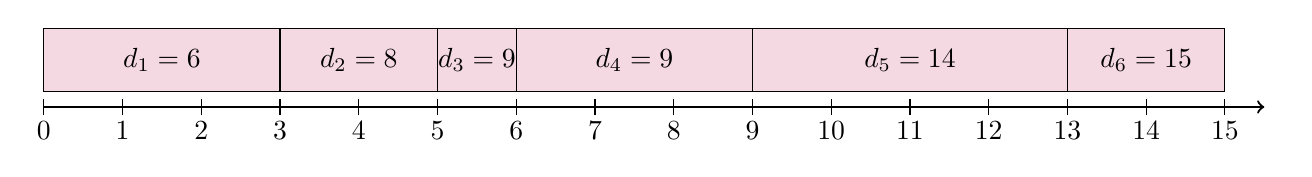
\begin{tikzpicture}
        % Draw the timeline
        \draw[thick,->] (0,0) -- (15.5,0) node[right] {};
        
        % Labels for time points
        \foreach \x in {0, 1, 2, 3, 4, 5, 6, 7, 8, 9, 10, 11, 12, 13, 14, 15} {
            \draw (\x,0.1) -- (\x,-0.1);
            \node at (\x,-0.3) {\x};
        }
        
        % Rectangles for jobs
        \filldraw[fill=purple!15] (0,0.2) rectangle (3,1);
        \node at (1.5,0.6) {$d_1 = 6$};
    
        \filldraw[fill=purple!15] (3,0.2) rectangle (5,1);
        \node at (4,0.6) {$d_2 = 8$};
    
        \filldraw[fill=purple!15] (5,0.2) rectangle (6,1);
        \node[inner sep=3pt] at (5.5,0.6) {$d_3 = 9$};
    
        \filldraw[fill=purple!15] (6,0.2) rectangle (9,1);
        \node at (7.5,0.6) {$d_4 = 9$};
    
        \filldraw[fill=purple!15] (9,0.2) rectangle (13,1);
        \node at (11,0.6) {$d_5 = 14$};
    
        \filldraw[fill=purple!15] (13,0.2) rectangle (15,1);
        \node at (14,0.6) {$d_6 = 15$};
        
    \end{tikzpicture}
    \caption{Where our number line represents time, and the rectangles the interval of each job.}
    \label{tab:late_sol}
\end{figure}

\noindent
Here we observe that we at most have $1$ late job.



% \chapter{Greedy Algorithms}
% \vspace{-1.5em}
\section{Dijkstra's Algorithm - Shortest Path}
\begin{theo}[Dijkstra's Algorithm]
    
    \textbf{Proposition:} Suppose that there is a shortest path from nodes $u\to v$. Then any
    sub-path between these nodes, say $x\to y$, is also the shortest path.\\

    \noindent
    \textbf{Algorithm:} Given a weighted graph $G$ and a source node $s$, 
    \begin{enumerate}
        \item [(i.)] Keep track of best distances, start at a queue with $s$.
        \item [(ii.)] Pop off the queue, flag item as visited.
        \item [(iii.)] View all children weights, update if it's the new shortest path to that node.
        \item [(iv.)] Queue children in ascending order of weight (smallest$\to$largest)
    \end{enumerate}
    Preform steps (ii) to (iv) until the queue is empty, having visited all possible nodes.
\end{theo}


\vspace{-1em}
\begin{Proof}[Proof of Correctness for Dijkstra's Algorithm]

    \textbf{Invariant:} For each node $u \in S$, $d(u)$ is length of shortest path $s \leadsto u$. By induction on $|S|$:\\
    \textbf{Base case:} $|S| = 1$ is true since $S = \{s\}$ and $d(s) = 0$.\\
    \textbf{Inductive hypothesis:} Assume true for $|S| = k \geq 1$.
    \begin{itemize}
        \item Let $v$ be the next node added to $S$, and let $(u, v)$ be the final edge.
        \item A shortest $s \leadsto u$ path plus $(u, v)$ is an $s \leadsto v$ path of length $\pi(v)$.
        \item Consider any $s \leadsto v$ path $P$. We show that it is no shorter than $\pi(v)$.
        \item Let $(x, y)$ be the first edge in $P$ that leaves $S$, and let $P'$ be the subpath to $x$.
        \item $P$ is already too long as soon as it reaches $y$.
    \end{itemize}
    \[
    \ell(P) \geq \ell(P') + \ell(x, y) \geq d(x) + \ell(x, y) \geq \pi(y) \geq \pi(v)
    \]
    \end{Proof}
    
\newpage

\noindent
To visualize our proof consider paths the following diagram:
\begin{figure}[h]
    \begin{center}
      \includegraphics[height=1.3in]{./Sections/dstra/dstra_proof.png}
    \end{center}
     \caption{A system of subset paths (blue), and an exact point of exit $u\to v$ and $x\to y$}\label{fig:dstra_proof}
\end{figure}

\noindent
Since $u\to y$ and $x\to y$ are at the same exact point of exit, i.e., say $s\to v\cong s\to y$, then to go from $y\to v$ must take some additional step.
Therefore, $s\to y\to v$ is longer. \textbf{E.g:} Let $s\to y:= 3$ and $s\to v:= 3$, and all steps take $1$.
Then $s\to y\to v = 4$, while $s\to v = 3$. Therefore $s\to v$ is the shortest path.\\

\noindent
\textbf{Dijkstra Example (i):} To emphasize the BFS nature of Dijkstra's algorithm:
\begin{figure}[h]
    
    \centering
    \tikzset{every picture/.style={line width=0.75pt}} %set default line width to 0.75pt        

    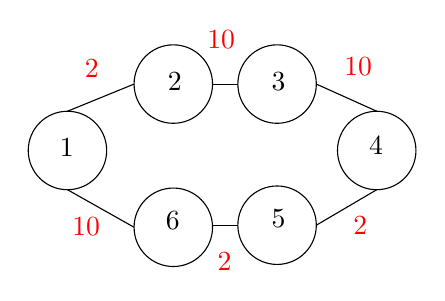
\begin{tikzpicture}[x=0.75pt,y=0.75pt,yscale=-1,xscale=1]
    %uncomment if require: \path (0,300); %set diagram left start at 0, and has height of 300

    %Shape: Circle [id:dp7522181001310076] 
    \draw   (171,142.9) .. controls (171,132.46) and (179.46,124) .. (189.9,124) .. controls (200.34,124) and (208.8,132.46) .. (208.8,142.9) .. controls (208.8,153.34) and (200.34,161.8) .. (189.9,161.8) .. controls (179.46,161.8) and (171,153.34) .. (171,142.9) -- cycle ;
    %Shape: Circle [id:dp46823217732954925] 
    \draw   (222,179.9) .. controls (222,169.46) and (230.46,161) .. (240.9,161) .. controls (251.34,161) and (259.8,169.46) .. (259.8,179.9) .. controls (259.8,190.34) and (251.34,198.8) .. (240.9,198.8) .. controls (230.46,198.8) and (222,190.34) .. (222,179.9) -- cycle ;
    %Shape: Circle [id:dp7637679019155722] 
    \draw   (222,110.9) .. controls (222,100.46) and (230.46,92) .. (240.9,92) .. controls (251.34,92) and (259.8,100.46) .. (259.8,110.9) .. controls (259.8,121.34) and (251.34,129.8) .. (240.9,129.8) .. controls (230.46,129.8) and (222,121.34) .. (222,110.9) -- cycle ;
    %Shape: Circle [id:dp70217655069576] 
    \draw   (272,178.9) .. controls (272,168.46) and (280.46,160) .. (290.9,160) .. controls (301.34,160) and (309.8,168.46) .. (309.8,178.9) .. controls (309.8,189.34) and (301.34,197.8) .. (290.9,197.8) .. controls (280.46,197.8) and (272,189.34) .. (272,178.9) -- cycle ;
    %Shape: Circle [id:dp2788867666411141] 
    \draw   (272,110.9) .. controls (272,100.46) and (280.46,92) .. (290.9,92) .. controls (301.34,92) and (309.8,100.46) .. (309.8,110.9) .. controls (309.8,121.34) and (301.34,129.8) .. (290.9,129.8) .. controls (280.46,129.8) and (272,121.34) .. (272,110.9) -- cycle ;
    %Shape: Circle [id:dp7250177070917547] 
    \draw   (320,142.9) .. controls (320,132.46) and (328.46,124) .. (338.9,124) .. controls (349.34,124) and (357.8,132.46) .. (357.8,142.9) .. controls (357.8,153.34) and (349.34,161.8) .. (338.9,161.8) .. controls (328.46,161.8) and (320,153.34) .. (320,142.9) -- cycle ;
    %Straight Lines [id:da06991122166773422] 
    \draw    (222,110.9) -- (189.9,124) ;
    %Straight Lines [id:da17655964402262492] 
    \draw    (222,179.9) -- (189.9,161.8) ;
    %Straight Lines [id:da8882356134150406] 
    \draw    (259.8,110.9) -- (272,110.9) ;
    %Straight Lines [id:da06318270683409766] 
    \draw    (259.8,178.9) -- (272,178.9) ;
    %Straight Lines [id:da3005609764749789] 
    \draw    (309.8,178.9) -- (338.9,161.8) ;
    %Straight Lines [id:da8117715540109972] 
    \draw    (309.8,110.9) -- (338.9,124) ;

    % Text Node
    \draw (185,136) node [anchor=north west][inner sep=0.75pt]   [align=left] {1};
    % Text Node
    \draw (237,104) node [anchor=north west][inner sep=0.75pt]   [align=left] {2};
    % Text Node
    \draw (287,104) node [anchor=north west][inner sep=0.75pt]   [align=left] {3};
    % Text Node
    \draw (334,135) node [anchor=north west][inner sep=0.75pt]   [align=left] {4};
    % Text Node
    \draw (287,170) node [anchor=north west][inner sep=0.75pt]   [align=left] {5};
    % Text Node
    \draw (236,171) node [anchor=north west][inner sep=0.75pt]   [align=left] {6};
    % Text Node
    \draw (256,84) node [anchor=north west][inner sep=0.75pt]   [align=left] {\textcolor[rgb]{1,0,0}{10}};
    % Text Node
    \draw (322,97) node [anchor=north west][inner sep=0.75pt]   [align=left] {\textcolor[rgb]{1,0,0}{10}};
    % Text Node
    \draw (197,98) node [anchor=north west][inner sep=0.75pt]   [align=left] {\textcolor[rgb]{1,0,0}{2}};
    % Text Node
    \draw (191,174) node [anchor=north west][inner sep=0.75pt]   [align=left] {\textcolor[rgb]{1,0,0}{10}};
    % Text Node
    \draw (261,191) node [anchor=north west][inner sep=0.75pt]   [align=left] {\textcolor[rgb]{1,0,0}{2}};
    % Text Node
    \draw (326.35,173.35) node [anchor=north west][inner sep=0.75pt]   [align=left] {\textcolor[rgb]{1,0,0}{2}};


    \end{tikzpicture}

     \caption{A weighted graph with shortest paths.}\label{fig:dstra_ex1}
\end{figure}

\vspace{-.5em}
\noindent
Where iterations and the queue look like:

\vspace{-1em}
$$\begin{matrix} \text{Iteration Init}&\text{from 1} & \text{from 2} & \text{from 6}&\text{from 3}&\text{from 5}\\ 1:0&1:0&1:0&1:0&1:0&1:0\\ 2:\infty&\textcolor{red}{2:2}&2:2&2:2&2:2&2:2\\ 3:\infty&3:\infty&\textcolor{red}{3:12}&3:12&3:12&3:12\\ 4:\infty&4:\infty&4:\infty&4:\infty&\textcolor{red}{4:22}&\textcolor{red}{4:14}\\ 5:\infty&5:\infty&5:\infty&\textcolor{red}{5:12}&5:12&5:12\\ 6:\infty&\textcolor{red}{6:10}&6:10&6:10&6:10&6:10\\ \end{matrix} $$
$$\begin{matrix} \text{Queue Init}&\text{from 1} & \text{from 2} & \text{from 6}&\text{from 3}&\text{from 5}\\ [1]&[2,6]&[6,3]&[3,5]&[5,4]&[4] \end{matrix}$$

\noindent
Finally visiting 4 to see 3 and 5 have already been visited, ending the algorithm as the queue's empty.


\newpage

\noindent
\textbf{Dijkstra Example (ii):}\\

\begin{figure}[h!]
    \centering
    \includegraphics[width=0.45\textwidth]{./Sections/dstra/w_dist.png} % First image
    \hfill % Adds space between the images
    \includegraphics[width=0.45\textwidth]{./Sections/dstra/w_graph.png} % Second image
    \caption{A weighted graph and its shortest paths.}
    \label{fig:combined_figure}
\end{figure}


\noindent
In figure (\ref{fig:combined_figure}), the first row is $0$ as $s\to s$, other nodes are assumed $\infty$,i.e., undefined. Each subsequent row finds the next shortest path, while 
updating the table about information it gathers.\\
\noindent
However we have one problem with Dijkstra's algorithm, it does not work with negative weights.
\begin{theo}[Dijkstra's Algorithm and Negative Weights]
    
    Dijkstra's algorithm does not work with negative weights. This is because it assumes that the shortest path is the sum of the shortest paths. Therefore,
    if the algorithm believes it has found the shortest path, it assumes any further traversals will only increase the path length.
\end{theo}


\noindent
To illustrate the deterioration of Dijkstra's algorithm:

\begin{figure}[h]
    \begin{center}
      \includegraphics[height=1.5in]{./Sections/dstra/dstra_neg.png}
    \end{center}
     \caption{Shows two weighted graphs, one positive, and the other negative.}\label{fig:dstra_neg}
\end{figure}

\noindent
In Figure (\ref{fig:dstra_neg}), our negative graph will never figure out the shortest path ($s\to b\to c\to a$=1). It 
will always assume $(s\to b\to a=3)$ is the shortest path. As when it looks at $c=4$, it will think that it's 
impossible to yield any shorter of a path $3$ as anything beyond $4$ must be larger.

\newpage
\begin{Func}[Dijkstra Algorithm - \texttt{Dijkstra($G, s$)}]

    Finds the shortest path in a weighted directed graph.

    \vspace{.5em}
    \noindent
    \textbf{Input:} A graph $G = (V, E)$ with adjacency list $G[u][v] = l(u, v)$ and source node $s$.\\
    \textbf{Output:} Shortest distances $d[u]$ and parent nodes for paths.

    \begin{algorithm}[H]
        \SetAlgoLined
        \SetKwProg{Fn}{Function}{:}{\KwRet{$d, parents$}}
        \Fn{\texttt{Dijkstra($G, s$)}}{
            $\pi \gets \{\}$\tcp{hash table, current best list for $v$}
            $d \gets \{\}$\tcp{hash table, distance of $v$}
            $parents \gets \{\}$\tcp{parents in shortest path tree}
            $Q \gets \text{PQ()}$\tcp{priority queue to track minimum $\pi$}

            $\pi[s] \gets 0$\;
            $Q.\texttt{INSERT}(\langle 0, s \rangle)$\;

            \For{$v \neq s$ in $G$}{
                $\pi[v] \gets \infty$\;
                $Q.\texttt{INSERT}(\langle \pi[v], v \rangle)$\;
            }

            \While{$Q$ is not empty}{
                $\langle \pi[u], u \rangle \gets \texttt{EXTRACT-MIN}(Q)$\;
                $d[u] \gets \pi[u]$\;
                \For{$v \in G[u]$}{
                    \If{$\pi[v] > d[u] + l(u, v)$}{
                        $\texttt{DECREASE-KEY}(\langle \pi[v], v \rangle, \langle d[u] + l(u, v), v \rangle)$\;
                        $\pi[v] \gets d[u] + l(u, v)$\;
                        $parents[v] \gets u$\;
                    }
                }
            }
        }
    \end{algorithm}

    \noindent
    \textbf{Time Complexity:} $O(m\log n)$ where $m$ is the number of edges and $n$ is the number of nodes, assuming $G$ is connected $(n-1\leq m)$; Otherwise,
    $O((n+m)\log n)$.\\
    \textbf{Space Complexity:} $O(n+m)$ storing the hash-table of the graph and priority queue.
\end{Func}

% \newpage 
\section{Spanning trees}

\begin{Def}[Spanning Tree]

    A \textbf{spanning tree} of a graph $G$ is a subgraph containing edges to each $n\in G$ without cycles.
\end{Def}

\begin{Def}[Minimum Spanning Tree (MST)]

    A \textbf{minimum spanning tree} of a graph $G$ is a spanning tree with the smallest sum of edge weights.
\end{Def}

\begin{figure}[h]
    \centering
    



    \tikzset{every picture/.style={line width=0.75pt}} %set default line width to 0.75pt        

    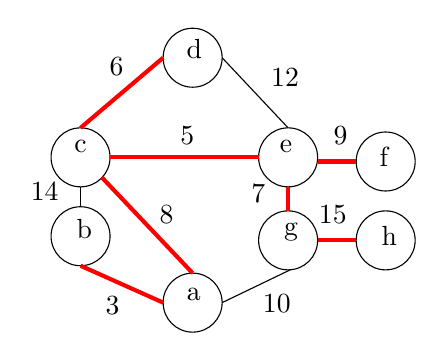
\begin{tikzpicture}[x=0.75pt,y=0.75pt,yscale=-1,xscale=1]
    %uncomment if require: \path (0,300); %set diagram left start at 0, and has height of 300
    
    %Shape: Circle [id:dp2026334324662925] 
    \draw  [fill={rgb, 255:red, 255; green, 255; blue, 255 }  ,fill opacity=1 ] (173.33,153.21) .. controls (173.33,145.36) and (179.69,139) .. (187.54,139) .. controls (195.39,139) and (201.75,145.36) .. (201.75,153.21) .. controls (201.75,161.06) and (195.39,167.42) .. (187.54,167.42) .. controls (179.69,167.42) and (173.33,161.06) .. (173.33,153.21) -- cycle ;
    %Shape: Circle [id:dp026171578812805518] 
    \draw  [fill={rgb, 255:red, 255; green, 255; blue, 255 }  ,fill opacity=1 ] (173.33,115.21) .. controls (173.33,107.36) and (179.69,101) .. (187.54,101) .. controls (195.39,101) and (201.75,107.36) .. (201.75,115.21) .. controls (201.75,123.06) and (195.39,129.42) .. (187.54,129.42) .. controls (179.69,129.42) and (173.33,123.06) .. (173.33,115.21) -- cycle ;
    %Shape: Circle [id:dp2560123313690592] 
    \draw  [fill={rgb, 255:red, 255; green, 255; blue, 255 }  ,fill opacity=1 ] (227.33,185.21) .. controls (227.33,177.36) and (233.69,171) .. (241.54,171) .. controls (249.39,171) and (255.75,177.36) .. (255.75,185.21) .. controls (255.75,193.06) and (249.39,199.42) .. (241.54,199.42) .. controls (233.69,199.42) and (227.33,193.06) .. (227.33,185.21) -- cycle ;
    %Shape: Circle [id:dp08670120448085128] 
    \draw  [fill={rgb, 255:red, 255; green, 255; blue, 255 }  ,fill opacity=1 ] (227.33,67.21) .. controls (227.33,59.36) and (233.69,53) .. (241.54,53) .. controls (249.39,53) and (255.75,59.36) .. (255.75,67.21) .. controls (255.75,75.06) and (249.39,81.42) .. (241.54,81.42) .. controls (233.69,81.42) and (227.33,75.06) .. (227.33,67.21) -- cycle ;
    %Shape: Circle [id:dp6890620040174518] 
    \draw  [fill={rgb, 255:red, 255; green, 255; blue, 255 }  ,fill opacity=1 ] (273.33,115.21) .. controls (273.33,107.36) and (279.69,101) .. (287.54,101) .. controls (295.39,101) and (301.75,107.36) .. (301.75,115.21) .. controls (301.75,123.06) and (295.39,129.42) .. (287.54,129.42) .. controls (279.69,129.42) and (273.33,123.06) .. (273.33,115.21) -- cycle ;
    %Shape: Circle [id:dp062427767698108316] 
    \draw  [fill={rgb, 255:red, 255; green, 255; blue, 255 }  ,fill opacity=1 ] (273.33,155.21) .. controls (273.33,147.36) and (279.69,141) .. (287.54,141) .. controls (295.39,141) and (301.75,147.36) .. (301.75,155.21) .. controls (301.75,163.06) and (295.39,169.42) .. (287.54,169.42) .. controls (279.69,169.42) and (273.33,163.06) .. (273.33,155.21) -- cycle ;
    %Shape: Circle [id:dp4615260186128455] 
    \draw   (320.33,155.21) .. controls (320.33,147.36) and (326.69,141) .. (334.54,141) .. controls (342.39,141) and (348.75,147.36) .. (348.75,155.21) .. controls (348.75,163.06) and (342.39,169.42) .. (334.54,169.42) .. controls (326.69,169.42) and (320.33,163.06) .. (320.33,155.21) -- cycle ;
    %Shape: Circle [id:dp46014483622543756] 
    \draw  [fill={rgb, 255:red, 255; green, 255; blue, 255 }  ,fill opacity=1 ] (320.33,117.21) .. controls (320.33,109.36) and (326.69,103) .. (334.54,103) .. controls (342.39,103) and (348.75,109.36) .. (348.75,117.21) .. controls (348.75,125.06) and (342.39,131.42) .. (334.54,131.42) .. controls (326.69,131.42) and (320.33,125.06) .. (320.33,117.21) -- cycle ;
    %Straight Lines [id:da8329795884294181] 
    \draw    (187.54,139) -- (187.54,129.42) ;
    %Straight Lines [id:da27990445195837865] 
    \draw [color={rgb, 255:red, 255; green, 0; blue, 0 }  ,draw opacity=1 ][line width=1.5]    (227.33,67.21) -- (187.54,101) ;
    %Straight Lines [id:da6849646426209853] 
    \draw [color={rgb, 255:red, 255; green, 0; blue, 0 }  ,draw opacity=1 ][line width=1.5]    (227.33,185.21) -- (187.54,167.42) ;
    %Straight Lines [id:da17487697052764262] 
    \draw [color={rgb, 255:red, 255; green, 0; blue, 0 }  ,draw opacity=1 ][line width=1.5]    (201.75,115.21) -- (273.33,115.21) ;
    %Straight Lines [id:da6321202969865173] 
    \draw [color={rgb, 255:red, 255; green, 0; blue, 0 }  ,draw opacity=1 ][line width=1.5]    (197.75,124.82) -- (241.54,171) ;
    %Straight Lines [id:da8393601584465114] 
    \draw    (255.75,185.21) -- (288.54,169.42) ;
    %Straight Lines [id:da8447960149171586] 
    \draw [color={rgb, 255:red, 255; green, 0; blue, 0 }  ,draw opacity=1 ][line width=1.5]    (287.54,141) -- (287.54,129.42) ;
    %Straight Lines [id:da3450940906788029] 
    \draw [color={rgb, 255:red, 255; green, 0; blue, 0 }  ,draw opacity=1 ][line width=1.5]    (320.33,155.21) -- (301.75,155.21) ;
    %Straight Lines [id:da8922618638234496] 
    \draw [color={rgb, 255:red, 255; green, 0; blue, 0 }  ,draw opacity=1 ][line width=1.5]    (320.33,117.21) -- (301.75,117.21) ;
    %Straight Lines [id:da7285203318813096] 
    \draw    (287.54,101) -- (255.75,67.21) ;
    
    % Text Node
    \draw (200.33,66) node [anchor=north west][inner sep=0.75pt]   [align=left] {6};
    % Text Node
    \draw (234.33,99) node [anchor=north west][inner sep=0.75pt]   [align=left] {5};
    % Text Node
    \draw (224.33,137) node [anchor=north west][inner sep=0.75pt]   [align=left] {8};
    % Text Node
    \draw (162.33,126) node [anchor=north west][inner sep=0.75pt]   [align=left] {14};
    % Text Node
    \draw (198.33,181) node [anchor=north west][inner sep=0.75pt]   [align=left] {3};
    % Text Node
    \draw (274.15,180.31) node [anchor=north west][inner sep=0.75pt]   [align=left] {10};
    % Text Node
    \draw (301.15,137.31) node [anchor=north west][inner sep=0.75pt]   [align=left] {15};
    % Text Node
    \draw (308.15,99.31) node [anchor=north west][inner sep=0.75pt]   [align=left] {9};
    % Text Node
    \draw (278.15,71.31) node [anchor=north west][inner sep=0.75pt]   [align=left] {12};
    % Text Node
    \draw (237.33,177) node [anchor=north west][inner sep=0.75pt]   [align=left] {a};
    % Text Node
    \draw (184.33,144) node [anchor=north west][inner sep=0.75pt]   [align=left] {b};
    % Text Node
    \draw (183.33,106) node [anchor=north west][inner sep=0.75pt]   [align=left] {c};
    % Text Node
    \draw (237.33,57) node [anchor=north west][inner sep=0.75pt]   [align=left] {d};
    % Text Node
    \draw (282.33,106) node [anchor=north west][inner sep=0.75pt]   [align=left] {e};
    % Text Node
    \draw (330.33,109) node [anchor=north west][inner sep=0.75pt]   [align=left] {f};
    % Text Node
    \draw (284.33,146) node [anchor=north west][inner sep=0.75pt]   [align=left] {g};
    % Text Node
    \draw (331.33,147) node [anchor=north west][inner sep=0.75pt]   [align=left] {h};
    % Text Node
    \draw (268.6,127) node [anchor=north west][inner sep=0.75pt]   [align=left] {7};
    
    
    \end{tikzpicture}

    \caption{Example of an graph with MST highlighted in red.}
    \label{fig:mst_example}

\end{figure}
\noindent
This tree visits each node once taking the shortest path which connects all of them.

\noindent
\textbf{Possible Algorithms:}
\begin{itemize}
    \item \textbf{Prim's:} Start with some root node s. Grow a tree T from s outward. At each step, add to T the cheapest edge e with exactly one endpoint in T.
    \item \textbf{Kruskal's:} Start with \( T = \emptyset \). Consider edges in ascending order of weights. Insert edge e in T unless doing so would create a cycle.
    \item \textbf{Reverse-Delete:} Start with \( T = E \). Consider edges in descending order of weights. Delete edge e from T unless doing so would disconnect T.
    \item \textbf{Borůvka's:} Start with \( T = \emptyset \). At each round, add the cheapest edge leaving each connected component of T. Terminates after at most \( \log(n) \) rounds.
\end{itemize}

\noindent
Next we revisit cycles and introduce \textbf{cuts}, which will have important implications when approaching this problem.

\newpage

\begin{Def}[Endpoint]
    
        An \textbf{endpoint} is either end of an edge. So for edge $e = u\leftrightarrow v$, $u$ and $v$ are endpoints. If
        $u\to v$, then $v$ is an endpoint of $u$.
\end{Def}
\begin{Def}[Cut]

    Given a graph $G$, partitioning of the nodes into a set is called a \textbf{cut}, say $G'$. Nodes, with exactly one endpoint in $G'$, are the \textbf{cut-set}.
    
\end{Def}



\begin{figure}[h]
    \centering
    

\tikzset{every picture/.style={line width=0.75pt}} %set default line width to 0.75pt        

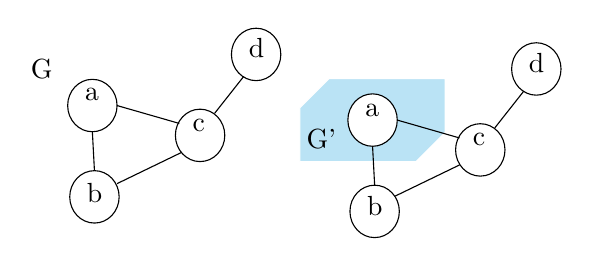
\begin{tikzpicture}[x=0.75pt,y=0.75pt,yscale=-1,xscale=1]
%uncomment if require: \path (0,265); %set diagram left start at 0, and has height of 265

%Snip Diagonal Corner Rect [id:dp03818061283377061] 
\draw  [color={rgb, 255:red, 255; green, 255; blue, 255 }  ,draw opacity=1 ][fill={rgb, 255:red, 96; green, 190; blue, 232 }  ,fill opacity=0.43 ] (263.9,142.63) -- (319.9,142.63) -- (319.9,142.63) -- (319.9,168.63) -- (305.9,182.63) -- (249.9,182.63) -- (249.9,182.63) -- (249.9,156.63) -- cycle ;
%Shape: Ellipse [id:dp6461843193531308] 
\draw   (138,155.63) .. controls (138,148.65) and (143.33,143) .. (149.9,143) .. controls (156.47,143) and (161.8,148.65) .. (161.8,155.63) .. controls (161.8,162.6) and (156.47,168.25) .. (149.9,168.25) .. controls (143.33,168.25) and (138,162.6) .. (138,155.63) -- cycle ;
%Shape: Ellipse [id:dp36167987939288815] 
\draw   (139,199.63) .. controls (139,192.65) and (144.33,187) .. (150.9,187) .. controls (157.47,187) and (162.8,192.65) .. (162.8,199.63) .. controls (162.8,206.6) and (157.47,212.25) .. (150.9,212.25) .. controls (144.33,212.25) and (139,206.6) .. (139,199.63) -- cycle ;
%Shape: Ellipse [id:dp21386485914880626] 
\draw   (189.9,170) .. controls (189.9,163.03) and (195.23,157.38) .. (201.8,157.38) .. controls (208.37,157.38) and (213.7,163.03) .. (213.7,170) .. controls (213.7,176.97) and (208.37,182.63) .. (201.8,182.63) .. controls (195.23,182.63) and (189.9,176.97) .. (189.9,170) -- cycle ;
%Straight Lines [id:da11599175466120859] 
\draw    (161.8,155.63) -- (191.8,164.25) ;
%Straight Lines [id:da8317457413146321] 
\draw    (149.9,168.25) -- (150.9,187) ;
%Shape: Ellipse [id:dp995295032837351] 
\draw  [fill={rgb, 255:red, 255; green, 255; blue, 255 }  ,fill opacity=1 ] (273,162.63) .. controls (273,155.65) and (278.33,150) .. (284.9,150) .. controls (291.47,150) and (296.8,155.65) .. (296.8,162.63) .. controls (296.8,169.6) and (291.47,175.25) .. (284.9,175.25) .. controls (278.33,175.25) and (273,169.6) .. (273,162.63) -- cycle ;
%Shape: Ellipse [id:dp8597498314367041] 
\draw   (274,206.63) .. controls (274,199.65) and (279.33,194) .. (285.9,194) .. controls (292.47,194) and (297.8,199.65) .. (297.8,206.63) .. controls (297.8,213.6) and (292.47,219.25) .. (285.9,219.25) .. controls (279.33,219.25) and (274,213.6) .. (274,206.63) -- cycle ;
%Shape: Ellipse [id:dp24205568125740362] 
\draw   (324.9,177) .. controls (324.9,170.03) and (330.23,164.38) .. (336.8,164.38) .. controls (343.37,164.38) and (348.7,170.03) .. (348.7,177) .. controls (348.7,183.97) and (343.37,189.63) .. (336.8,189.63) .. controls (330.23,189.63) and (324.9,183.97) .. (324.9,177) -- cycle ;
%Straight Lines [id:da5757559450680038] 
\draw    (296.8,162.63) -- (326.8,171.25) ;
%Straight Lines [id:da9921369924680631] 
\draw    (284.9,175.25) -- (285.9,194) ;
%Straight Lines [id:da696315279326696] 
\draw    (161.8,193.25) -- (192.8,178.25) ;
%Straight Lines [id:da9313904515500769] 
\draw    (295.8,199.25) -- (326.8,184.25) ;
%Shape: Ellipse [id:dp6136012462910496] 
\draw   (216.9,131) .. controls (216.9,124.03) and (222.23,118.38) .. (228.8,118.38) .. controls (235.37,118.38) and (240.7,124.03) .. (240.7,131) .. controls (240.7,137.97) and (235.37,143.63) .. (228.8,143.63) .. controls (222.23,143.63) and (216.9,137.97) .. (216.9,131) -- cycle ;
%Straight Lines [id:da5907253154079168] 
\draw    (222.8,141.63) -- (208.8,159.38) ;
%Shape: Ellipse [id:dp9497617675815347] 
\draw   (351.9,138) .. controls (351.9,131.03) and (357.23,125.38) .. (363.8,125.38) .. controls (370.37,125.38) and (375.7,131.03) .. (375.7,138) .. controls (375.7,144.97) and (370.37,150.63) .. (363.8,150.63) .. controls (357.23,150.63) and (351.9,144.97) .. (351.9,138) -- cycle ;
%Straight Lines [id:da7693110411499856] 
\draw    (357.8,148.63) -- (343.8,166.38) ;

% Text Node
\draw (145,146) node [anchor=north west][inner sep=0.75pt]   [align=left] {a};
% Text Node
\draw (146,192) node [anchor=north west][inner sep=0.75pt]   [align=left] {b};
% Text Node
\draw (197,161) node [anchor=north west][inner sep=0.75pt]   [align=left] {c};
% Text Node
\draw (280,154) node [anchor=north west][inner sep=0.75pt]   [align=left] {a};
% Text Node
\draw (332,168) node [anchor=north west][inner sep=0.75pt]   [align=left] {c};
% Text Node
\draw (281,198) node [anchor=north west][inner sep=0.75pt]   [align=left] {b};
% Text Node
\draw (119,132) node [anchor=north west][inner sep=0.75pt]   [align=left] {G};
% Text Node
\draw (251.9,165.63) node [anchor=north west][inner sep=0.75pt]   [align=left] {G'};
% Text Node
\draw (224,122) node [anchor=north west][inner sep=0.75pt]   [align=left] {d};
% Text Node
\draw (359,129) node [anchor=north west][inner sep=0.75pt]   [align=left] {d};


\end{tikzpicture}

    \caption{Illustration of a graph $G$ and a cut $G'$ of the graph.}
    \label{fig:cut_example}
\end{figure}
\noindent
We see in Figure (\ref{fig:cut_example}) that $G'=\{a\}$ and our cut-set contains edge-pairs $(a,b)$ and $(a,c)$. Where the edge $(d,c)$ is not included as the cut $G'$ does not intersect it.
\begin{theo}[Cycles \& Cut-sets]

    If a cut-set crosses a cycle, then the cut-set intersects an even number of edges in the cycle.\\
    As what comes in, must come out.
\end{theo}
\noindent
Given Figure (\ref{fig:cut_example}), the cut-set $G'$ intersects the cycle $(a,b,c)$, yielding an even cut-set.
\begin{theo}[Cycle Property]
    
    In a graph with a cycle, the edge with the largest weight in that cycle is not in the MST.
    As taking an edge from a cycle does not disconnect the graph, the largest edge is not necessary.
\end{theo}
\begin{theo}[Cut Property]

    Given a graph $G$ and a cut-set $C$, where $e$ is the lightest-edge in $C$; $e$ must be in the MST. As if $e\notin G$ and $G$ is an MST, adding $e$ creates a cycle. By the cycle property, $e$ must replace the heaviest edge in that cycle.
\end{theo}


\newpage
\noindent
\textbf{Example:} Given the below Figure (\ref{fig:cut_property}), point $e$ must be in the MST to connect all nodes (cut property). Say dash-edge $f$ is the largest in its cycle, then $f$ is not in the MST (cycle property).
\begin{figure}[h]
    \centering
    

\tikzset{every picture/.style={line width=0.75pt}} %set default line width to 0.75pt        

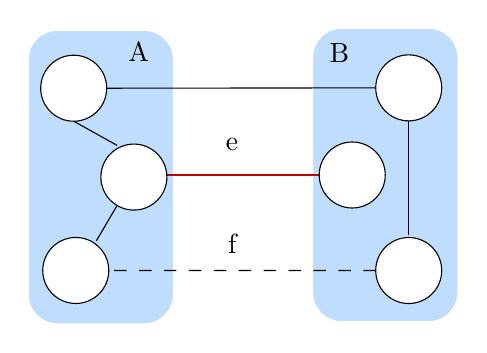
\begin{tikzpicture}[x=0.75pt,y=0.75pt,yscale=-1,xscale=1]
%uncomment if require: \path (0,300); %set diagram left start at 0, and has height of 300

%Rounded Rect [id:dp49102406805739185] 
\draw  [color={rgb, 255:red, 255; green, 255; blue, 255 }  ,draw opacity=1 ][fill={rgb, 255:red, 139; green, 194; blue, 255 }  ,fill opacity=0.56 ] (166,94) .. controls (166,86.27) and (172.27,80) .. (180,80) -- (222,80) .. controls (229.73,80) and (236,86.27) .. (236,94) -- (236,207.42) .. controls (236,215.15) and (229.73,221.42) .. (222,221.42) -- (180,221.42) .. controls (172.27,221.42) and (166,215.15) .. (166,207.42) -- cycle ;
%Rounded Rect [id:dp35224359948314676] 
\draw  [color={rgb, 255:red, 255; green, 255; blue, 255 }  ,draw opacity=1 ][fill={rgb, 255:red, 139; green, 194; blue, 255 }  ,fill opacity=0.56 ] (303,93) .. controls (303,85.27) and (309.27,79) .. (317,79) -- (359,79) .. controls (366.73,79) and (373,85.27) .. (373,93) -- (373,206.42) .. controls (373,214.15) and (366.73,220.42) .. (359,220.42) -- (317,220.42) .. controls (309.27,220.42) and (303,214.15) .. (303,206.42) -- cycle ;
%Straight Lines [id:da3016657209067013] 
\draw [color={rgb, 255:red, 195; green, 0; blue, 0 }  ,draw opacity=1 ]   (306.2,149.71) -- (232.8,149.71) ;
%Shape: Circle [id:dp005421762108458239] 
\draw  [fill={rgb, 255:red, 255; green, 255; blue, 255 }  ,fill opacity=1 ] (172,107.9) .. controls (172,99.12) and (179.12,92) .. (187.9,92) .. controls (196.68,92) and (203.8,99.12) .. (203.8,107.9) .. controls (203.8,116.68) and (196.68,123.8) .. (187.9,123.8) .. controls (179.12,123.8) and (172,116.68) .. (172,107.9) -- cycle ;
%Shape: Circle [id:dp4707156627783562] 
\draw  [fill={rgb, 255:red, 255; green, 255; blue, 255 }  ,fill opacity=1 ] (201,150.71) .. controls (201,141.93) and (208.12,134.81) .. (216.9,134.81) .. controls (225.68,134.81) and (232.8,141.93) .. (232.8,150.71) .. controls (232.8,159.49) and (225.68,166.61) .. (216.9,166.61) .. controls (208.12,166.61) and (201,159.49) .. (201,150.71) -- cycle ;
%Shape: Circle [id:dp7864251820189283] 
\draw  [fill={rgb, 255:red, 255; green, 255; blue, 255 }  ,fill opacity=1 ] (173,195.71) .. controls (173,186.93) and (180.12,179.81) .. (188.9,179.81) .. controls (197.68,179.81) and (204.8,186.93) .. (204.8,195.71) .. controls (204.8,204.49) and (197.68,211.61) .. (188.9,211.61) .. controls (180.12,211.61) and (173,204.49) .. (173,195.71) -- cycle ;
%Straight Lines [id:da6423097124480006] 
\draw    (208.8,164.43) -- (198.8,181.43) ;
%Straight Lines [id:da19288845816924016] 
\draw    (187.9,123.8) -- (208.8,135.43) ;
%Shape: Circle [id:dp4761241780620117] 
\draw  [fill={rgb, 255:red, 255; green, 255; blue, 255 }  ,fill opacity=1 ] (333.42,107.73) .. controls (333.42,98.95) and (340.54,91.83) .. (349.32,91.83) .. controls (358.1,91.83) and (365.22,98.95) .. (365.22,107.73) .. controls (365.22,116.51) and (358.1,123.63) .. (349.32,123.63) .. controls (340.54,123.63) and (333.42,116.51) .. (333.42,107.73) -- cycle ;
%Shape: Circle [id:dp6465860920913904] 
\draw  [fill={rgb, 255:red, 255; green, 255; blue, 255 }  ,fill opacity=1 ] (306.2,149.71) .. controls (306.2,140.93) and (313.32,133.81) .. (322.1,133.81) .. controls (330.88,133.81) and (338,140.93) .. (338,149.71) .. controls (338,158.49) and (330.88,165.61) .. (322.1,165.61) .. controls (313.32,165.61) and (306.2,158.49) .. (306.2,149.71) -- cycle ;
%Shape: Circle [id:dp2663185207581561] 
\draw  [fill={rgb, 255:red, 255; green, 255; blue, 255 }  ,fill opacity=1 ] (333.42,195.73) .. controls (333.42,186.95) and (340.54,179.83) .. (349.32,179.83) .. controls (358.1,179.83) and (365.22,186.95) .. (365.22,195.73) .. controls (365.22,204.51) and (358.1,211.63) .. (349.32,211.63) .. controls (340.54,211.63) and (333.42,204.51) .. (333.42,195.73) -- cycle ;
%Straight Lines [id:da6545330759865682] 
\draw  [dash pattern={on 4.5pt off 4.5pt}]  (333.42,195.73) -- (204.8,195.71) ;
%Straight Lines [id:da23327256965954069] 
\draw    (333.42,107.73) -- (203.8,107.9) ;
%Straight Lines [id:da6594941535881259] 
\draw    (349.32,123.63) -- (349.32,178.83) ;

% Text Node
\draw (260,131) node [anchor=north west][inner sep=0.75pt]   [align=left] {e};
% Text Node
\draw (213,84.48) node [anchor=north west][inner sep=0.75pt]   [align=left] {A};
% Text Node
\draw (310,85) node [anchor=north west][inner sep=0.75pt]   [align=left] {B};
% Text Node
\draw (261,177) node [anchor=north west][inner sep=0.75pt]   [align=left] {f};


\end{tikzpicture}
    
    \caption{A graph cut into two disjoint sets, with a highlighted edge $e$ and a dashed edge $f$.}
    \label{fig:cut_property}
\end{figure}

\vspace{-1em}
\begin{theo}[Prim's Algorithm]

    \label{theo:prim}
    Given a connected graph $G$ with $n$ nodes and $m$ edges, we produce the MST via:
    \begin{enumerate}
        \item [(i.)] Initialize an MST table $T$, and a priority queue $Q$ with each $n$ of weight $\infty$.
        \item [(ii.)] Start a round with an arbitrary node $s$, evaluating children nodes $v$.
        \item [(iii.)] Update each $T[v]=s$, if $w(s,v)$ is lighter than $T[v]$.
        \item [(iv.)] End this round, take the top node in $Q$ as the new $s$, repeat (ii.)-(iv.) until all $n\in T$.
    \end{enumerate}
    \noindent

\end{theo}

\vspace{-2em}
\begin{figure}[h]
    \centering
    \hfill
    \begin{minipage}{0.45\textwidth}
        \centering

        \vspace{2em}
      
        \includegraphics[height=2in]{./Sections/spanning/prims_order.png}
        
    \end{minipage}%
    \hfill
    \begin{minipage}{0.45\textwidth}
        \centering

        \vspace{2em}
        $$ \begin{matrix} 
        \text{NODE} & \text{PARENT}\\
        a: & \text{NULL}\\ 
        b: & a\\ 
        c: & a\\ 
        d: & c\\ 
        e: & c\\ 
        g: & e\\ 
        f: & e\\ 
        h: & g 
        \end{matrix} $$
    \end{minipage}
    \hfill 
    \caption{Prim's Alg. in the order $a\to b \to c \to e \to d \to g \to f \to h$, and a parent table.}
    \label{fig:prim_example}
\end{figure}

\noindent 
The above example shows how our parent table will result with the following table. Next we will discuss in detail how one could approach implementation.

\newpage
\begin{Tip}
    Live Demo of Prim's Algorithm \url{https://www.youtube.com/watch?v=cplfcGZmX7I}.
\end{Tip}

\vspace{-1em}
\begin{Func}[Prim's Algorithm - \texttt{PALG()}]
    \textbf{Input:} A connected, undirected graph \( G\) of $V$ nodes. With weights \( w(u, v) \), and $u,v\in V$.\\
    \textbf{Output:} Minimum Spanning Tree (MST) formed by edges \( T<(v, \texttt{parent}[v])> \)\\

    \vspace{-.5em}
    \begin{algorithm}[H]
        \label{algo:prim}
        $Q<weight, node>$; \tcp {Min-heap of <key, data>}
        $V.forEach$(($v$) => $\{Q[v]\gets \infty\}$); \tcp{for each $v\in V$ set it's weight to $\infty$}
        $Q[V_0]\gets 0$; \tcp{Picking arbitrary node $V_0$, pushing it to the top of $Q$}
        $T$; \tcp{Hashtable where $T[u]$ is the parent $v$ of $u$}
        
        \vspace{.5em}
        \While{\( Q \neq \emptyset \)}{
            $ u \gets Q.Extract() $\;

            \vspace{.5em}
            \ForEach{\(v \in G[u] \)}{
                    
                \vspace{.5em}
                \If{$(v\in Q)$ and $(w(u,v)<Q[v])$}
                {
                    \tcp{Edit the node's weight in $Q$ then re-balance.}
                    $Q[v]\gets w(u,v)$\;
                    $Q.DecreaseKey(v)$\;
                    $T[v]\gets u$\;
                }

            }
            
            % \For{each \( v \in G[u] \)}{
            %     \If{\( v \notin V \text{ and } w(u, v) < \texttt{key}[v] \)}{
            %         \( \texttt{key}[v] \gets w(u, v) \)\;
            %         \( \texttt{parent}[v] \gets u \)\;
            %         \( Q.\texttt{Decrease-Key}(v, \texttt{key}[v]) \)\;
            %     }
            % }
        }
        \KwRet{$T$}
    \end{algorithm}
    \noindent\rule{\textwidth}{0.4pt}

    \noindent
    \textbf{Correctness:} We run a form of BFS on the graph, which touches every node. BFS creates levels each iteration, resulting in a cut-set with an end-point $G[u]$.
    By the cut property, any new lightest edge $w(u,v)$ is added or replaces a heavier edge in $T$. Thus forming an MST as all nodes are considered.\\
    \textbf{Time Complexity:} $O((n+m)\log n)$. Line 7 at worse checks every adjacency, $O(n+m)$, for $m$ edges of $n$ nodes. 
    Say lines 8-9 takes $O(1)$ time to find $v\in Q$ via hash-table. Line 10 takes $O(\log n)$ time to re-balance the heap.
    Thus, $O((n+m)\log n)$ or $O(m\log n)$.\\
    \textbf{Space Complexity:} $O(n+m)$, as we at most store the data items a hash-table representation of our graph.
\end{Func}

\noindent
\underline{\textbf{Note:} Lines 8 to 10 may require additional implementation.} Since basic min-heaps only store weights, one 
might need a direct reference to each member in the heap. Say a reference hash-table $R$, where $R[v]$ 
points to $v$ node in $Q$. Once we update $R[v]$, we tell the $Q$ to sort the new $v$ weight. We say
``$DecreaseKey$'' as our new weight should be lighter, bubbling up the heap.\\

\noindent
To check if a node has been visited before, doesn't matter in our case, as we update our solution $T$ with 
a better solution once it is found. We additionally discard the lightest node each round to avoid infinite loops. If one wanted to, they could use $T$'s entries as a visited list. If entries are
undefined upon access, then they have not been visited.\\

\newpage 

\begin{figure}[h]
\centering

        

\tikzset{every picture/.style={line width=0.75pt}} %set default line width to 0.75pt        



\includegraphics[height=5in]{./Sections/spanning/prims_alg.png}

        \caption{A diagram illustrating the pattern of Prim's Algorithm through each iteration.}
        \label{fig:prim_example}
    \end{figure}



\noindent
The above diagram shows Prim's algorithm each round, pick the lightest edge at the top of the heap, check its degrees which have not been, 
update weights, re-balance the heap, and repeat. The algorithm will terminate when all nodes have been picked from the heap.\\ 

\newpage
\begin{Proof}[Prim's Hash-tables vs. Min-heaps Implementation]
    Say we had a hash-table of priorities where $R[v]$ returns weight $w(u,v)$:
    % Under light loads, a hash-table preforms better than a min-heap. However, under heavy loads, a min-heap.
    \begin{itemize}
        \item \textbf{Hash-table} - \textbf{Extract:} $O(n)$, search all indices, \textbf{Decrease-Key:} $O(1)$, update $R[v]$.
        \item \textbf{Min-heap} - \textbf{Extract:} $O(1)$, top element, \textbf{Decrease-Key:} $O(\log n)$, re-balance heap.
    \end{itemize}
    \begin{center}
    \includegraphics[height=2.3in]{./Sections/spanning/alg.png}
    \end{center}

    line 5 stores all $n$ nodes to be visited $O(n)$, line 7 iterates all neighbors for each $n$. Let all edges be $m$, then $\sum_{v \in n} \text{degree}(v)=m$.
    Since line 6 is $O(1)$, we have $O(n+m)$ for iterating all edges. Now for every edge, we might evaluate Decrease-Key, which is $O(\log n)$. This gives us 
    $O((n+m)\log n)$, or $O(m\log n)$.
    
    When using a hash-table, line 6 becomes $O(n)$, and Decrease-Key is $O(1)$. Thus,\\
    $O((n(n)+m)\cdot 1)= O(n^2+m)$ or $O(n^2)$. Hence,

    \begin{center}
        \textbf{Hash-table:} $O(n^2)$. \textbf{Min-heap:} $O(m\log n)$.\\
    \end{center}

    \noindent
    For any connected graph $n-1\leq m \leq \frac{n(n-1)}{2}$, where $m$ is the number of edges. Most often $m$ is much less than $n$, making the min-heap the better choice.
    E.g., say $m=\frac{n^2}{2}$, then $O(n^2)$ vs. $O(n^2\log n)$, hash-table wins. However, say $m=\frac{n}{2}$, then $O(n^2)$ vs. $O(n\log n)$, min-heap wins.
\end{Proof}

\begin{theo}[Prim's Hash-tables vs. Min-heaps]

    For Prim's algorithm,\\
    when $m \leq n$, min-heap is better ($O(n\log n)<O(n^2)$). When $m$ is significantly larger than $n$, hash-tables are better ($O(n^2)<O(n^2\log n)$).
\end{theo}
\newpage
\subsection{Union-Find Data Structures}
\begin{Def}[Union-Find Data Structure]

    A \textbf{Union-Find} data structure is a data structure that keeps track of a set of elements partitioned into multiple disjoint subsets. 
    It supports two useful operations: \textbf{Union:} Merge two subsets into a single subset. \textbf{Find:} Determine which subset a particular element is in.
\end{Def}

\noindent
We \textit{could} simply use a hash-table to keep track of the parent of each node, which gives us\\ 
\textbf{Find O(1); However, Union is $\mathbf{O(n)}$}, as we would have to update every node to its new parent. Given a large set of $n$ nodes, with $m$ edges in a hash-table, to find and union all $n$ nodes
results in \textbf{$\mathbf{O(n^2+m)}$}, as for every $n$ we find, we make $n$ updates, where our finds accumulate to the number of total edge connections.\\

\noindent
\textbf{Scenario - \textit{Follow The Leader:}}
Say you have $n$ people playing rock-paper-scissors. If $n_i$ beats $n_j$, then $n_j$ follows $n_i$. This 
creates large sets of people following a leader. When leader $n_k$ beats $n_i$, $n_i$ follows $n_k$ with $n_i$'s followers tagging along.\\

\noindent
Say we are trying to figure out which component $n_x$ is in. We ask $n_x$, ``who is your leader,'' they say $n_i$, then $n_i$ says $n_k$, and $n_k$ replies, ``I am the leader.'' 
Therefore $n_x$ is in group $n_k$.
\begin{Def}[Forest]

    A \textbf{forest} is a collection of disjoint trees, where each tree has a \textbf{representative} $r$ node. We may
    union-join trees $A$ and $B$ by making $A$ be $B$'s representative. Where $b\in B$ still point to $B$ and $B$ points to $A$.

    \underline{Trees $S$ with smaller heights should be added to bigger trees $B$.} As height indicates the number of nodes who report to a leader.
    By adding the bigger tree to the smaller, we increase the time complexity of finding leaf nodes.

\end{Def}

\vspace{-3.5em}
\begin{figure}[h]
    \centering
    \includegraphics[height=2.3in]{./Sections/spanning/forest-diag.png}
    
    \vspace{-2em}
    \caption{Showing disjoint nodes Union-Join with each other.}
    \label{fig:forest_diag}
\end{figure}

\noindent
In the above figure nodes we see in step two we have two disjoint trees, with leaders $a$ and $c$. In step three we join $a$ and $c$ by making $c$ point to $a$. Finally $e$ points to $a$ to join the group.\\

\noindent
We see a lot of redundancy, with nodes $n_x$ reporting to leaders $n_i$, until a final leader $n_k$ is reached. We may improve this overtime by setting $n_x$'s leader to $n_k$ directly.\\

\vspace{-3em}
\begin{figure}[h]
    \centering
    \includegraphics[height=2.3in]{./Sections/spanning/path_compression.png}
    
    \vspace{-1em}
    \caption{Showing a forest compress over multiple finds.}
    \label{fig:path_compression}
\end{figure}
\noindent
Given the figure above, we first ask $g$ who their leader is, they report to $c$ who reports to $a$. We now set $g$'s leader to $a$. We do the same for $f$ and $d$. Now once
we ask $g,f,$ or $d$ who their leader is, they report to $a$ directly without the need to traverse the tree. This is called \textbf{Path Compression}.
\begin{Def}[Path Compression]

    \textbf{Path Compression} is a technique used in Union-Find data structures to flatten the structure of the tree. 
    After finding the leader of a node in a whole component, we set the node's parent directly to that leader. This reduces the time complexity of find operations for subsequent queries.
\end{Def}

We compare all of our techniques in the following table:
\begin{table}[h!]
  \centering
  \resizebox{\textwidth}{!}{%
    \renewcommand{\arraystretch}{1.5}%
    \setlength{\tabcolsep}{5pt}%
    \rowcolors{2}{OliveGreen!5}{}%
    \begin{tabular}{>{\columncolor{OliveGreen!15}}l | c c c}
      \rowcolor{OliveGreen!20}
      Operation\textbackslash{}Implementation 
        & Simple Hash-table 
        & Forest 
        & \makecell[l]{\rule{0pt}{2.5ex}Forest with\\ Path Compression} \\
      \hline
      Find (worst-case)
        & $\Theta(1)$
        & $\Theta(\log n)$
        & $\Theta(\log n)$ \\ \hline
    \cellcolor{OliveGreen!15}Union of sets $A,B$ (worst-case)
        & $\Theta(n)$
        & $\Theta(1)$
        & $\Theta(1)$ \\ \hline
    \makecell[l]{\rule{0pt}{2.6ex} Total for $n$ unions and $n$ finds,\\ starting from singletons}
        & $\Theta(n^2)$
        & $\Theta(n\log n)$
        & $\Theta\bigl(m\cdot\alpha(m,n)\bigr)$ \\
    \end{tabular}%
  }
  \caption{Time-complexity comparison of different implementations. Where $\alpha(m,n)$ is the inverse Ackermann function, which grows very slowly.}
  \label{tab:uf-complexity}
\end{table}


\newpage
\noindent 

\begin{theo}[Kruskal's Algorithm]

    \label{theo:kruskal}
    Given a connected graph $G$ of $V$ nodes and $E$ edges, we produce the MST via:
    \begin{enumerate}
        \item [(i.)] Sort all $e\in E$ by weight in ascending order into an array $W$.
        \item [(ii.)] Initialize a forest $T$ with all $V$ nodes as singletons.
        \item [(iii.)] For each $e\in W$ Union-find its endpoints $u$ and $v$.
        \begin{itemize}
            \item If $u$ and $v$ are in different sets, Union-join $u$ and $v$.
        \end{itemize}
    \end{enumerate}
    \noindent
    Return the resulting forest $T$ as the MST.
\end{theo}

\begin{Func}[Kruskal's Algorithm - \texttt{KALG()}]
    \textbf{Input:} a connected graph $G$ of $V$ nodes and $E$ edges.\\
    \textbf{Output:} Minimum Spanning Tree (MST) formed by forest Union-find data structure.\\

    \vspace{-.5em}
    \begin{algorithm}[H]
        \label{algo:prim}
        $W[\ ]\gets Sort(E)$; \tcp {Sort all edges by weight}
        $T\gets new \ UnionFind(G)$; \tcp{new forest with all $G$'s nodes as singletons}

        \vspace{.5em}
        \For {$i=1$ to $W.size()$}{
            $(u,v)\gets e$; \tcp{Get the endpoints of $e$}

            \vspace{.5em}
            \If{$T.Find(u)\neq T.Find(v)$}{
                $T.Union(u,v)$; \tcp{Union-join $u$ and $v$}
            }
        }
        \KwRet{$T$}
    \end{algorithm}
    \noindent\rule{\textwidth}{0.4pt}

    \noindent
    \textbf{Correctness:} Sorting edges in ascending order, ensures lightest possible edge is picked first before redundancy checks with Union-find, which avoids cycles (Line 5).
    Any new unique edge $e$ is added to the MST. This yields a connected graph as all edges are considered no matter their weight.\\
    \textbf{Time Complexity:} $O(E \log E)$ or $O(E \log V)$. Line 1 sorts all edges, which takes $O(E \log E)$ time, where $E$ is at most $V^2$ (all nodes connect to each other).
    Thus, $\Theta(E \log_2 V)$ is $O(E \log_2 E)$ as the exponent to reach $V$ and $E$ are the same. Then iterating through all $E$ edges; 
    actions are one-to-one for each \textit{find-merge} operation $E_i$. This results in one operation per edge, rather than a compounded combination of operations, like a nested for-loops.\\
    \textbf{Space Complexity:} $O(V+E)$, as we at most store the data items a hash-table representation of our graph.
\end{Func}

\noindent
\textbf{Note:} Lines 1 and 4, might require additional implementation such as a reference hash-table $R$ to keep track of edges and their end-points after sorting.

\newpage

\begin{Exercise} Let there be a graph $G(V,E)$ with an MST $T$ and a shortest paths tree $S$. Now 
    suppose a weight of 1 is added to each edge in $G$.
\begin{enumerate}
    \item Will the MST $T$ change?
    \item Will the shortest paths tree $S$ change?
\end{enumerate}
\end{Exercise} 

\begin{Exercise} Let there be a graph $G(V,E)$ with an MST $T$ and a shortest paths tree $S$.
    Suppose a new edge $e$ is added to $G$.
    \begin{enumerate}
        \item The weight of $e$ is the heaviest in $G$.
            \begin{enumerate}
                \item Will the MST $T$ change?
                \item Will the shortest paths tree $S$ change?
            \end{enumerate}
        \item The weight of $e$ is the lightest in $G$.
            \begin{enumerate}
                \item Will the MST $T$ change?
                \item Will the shortest paths tree $S$ change?
            \end{enumerate}
    \end{enumerate}
\end{Exercise}

\noindent\rule{\textwidth}{0.4pt}

\vspace{1em}
\begin{Answer} 
    \begin{enumerate}
        \item \textbf{No.} All edges in $T$ are still the lightest edges in $G$.
        \item \textbf{Yes.} Shortest paths is not MST. Here is a counter example:\\
        \vspace{1em}
        \includegraphics[height=1in]{./Sections/spanning/counter.png}\\

        \vspace{-2em}
        \noindent
        The shortest path from $s$ to $t$ changed when all edges were increased by 1.
    \end{enumerate}
\end{Answer}

\begin{Answer} 
    \begin{enumerate}
        \item \begin{enumerate}
            \item \textbf{No.} By the cycle property, the heaviest edge is not necessary in the MST.
            \item \textbf{Yes.} The new edge may present a shorter path. Here is a counter example:\\
            \includegraphics[height=1.1in]{./Sections/spanning/counter_2.png}\\
        \end{enumerate}
        \item \begin{enumerate}
            \item \textbf{Yes.} By the cycle property, an existing edge will be replaced by a lighter edge.
            \item \textbf{Yes.} Consider a long expensive path, a new edge may present a shorter path.
        \end{enumerate}
    \end{enumerate}
    
\end{Answer}

% \chapter{Evaluating Recursive Algorithms}
% \vspace{-2em}
\section{Inductive Analysis}

Recursion employs techniques of repeatedly shrinking the problem to solve its smaller halves. Often found in sorting problems, processing trees, and
geometric problems.

\begin{theo}[MergeSort]
    
    Given an array $A$ of size $n$, we sort via the following:
    \begin{enumerate}
        \item [(i.)] Recursively: Split the array into two halves and wait for a return.
        \item [(ii.)] Base-case: If the array has one element, return it.
        \item [(iii.)] Merge: receive two halves and merge them.
    \end{enumerate}
    The final result is a sorted array.
\end{theo}

\begin{theo}[QuickSort]

    Given an array $A$ of size $n$, we sort via the following:
    \begin{enumerate}
        \item [(i.)] Choose a pivot, set $i$ to the start and $j$ at the end of the array.
        \item [(ii.)] Increase $i$ until $A[i]>pivot$ and decrease $j$ until $A[j]<pivot$.
        \begin{itemize}
            \item If $A[i]<A[j]$, swap $A[i]$ and $A[j]$.
            \item Repeat until $i>j$, return $j$ as the new pivot.
        \end{itemize}
        \item [(iii.)] The new pivot creates two sub-arrays, repeat the process on each sub-array.
    \end{enumerate}
    The final result is $A$ sorted in-place (on the original array without a temporary helper array).
\end{theo}

\begin{Tip} Demos for 
 \textbf{MergeSort}: \url{https://youtu.be/ZLBmc0qf174?si=2b0Kxy9xxPHos_6A} and\\
 \textbf{QuickSort}: \url{https://youtu.be/FWWqLJIUFZM?si=ZPhuvIduWAGXH_mv}.
\end{Tip}

\newpage

\begin{Func}[Mergesort - \texttt{MSORT(A)}]
    \textbf{Input:} Array $A$ and temporary array $temp$ of $n$ elements.\\
    \textbf{Output:} Nothing is returned, the array $A$ is sorted by reference.\\

    \vspace{-.5em}
    \noindent
    \textbf{MSORT function}\textit{(A,temp,i,j)}:\\
    \begin{algorithm}[H]
        \label{algo:mergesort}
        \If{$i \geq j$}{
            \Return;
        }
            $mid \gets (i + j) / 2$\;
            $MSORT(A, temp, i, mid);$ \tcp{Left subarray}
            $MSORT(A, temp, mid + 1, j);$ \tcp{Right subarray}
            $merge(A, temp, i, mid, mid + 1, j);$ \tcp{Merge both halves}
        
    \end{algorithm}

    \vspace{.5em}

    \noindent
    \textbf{Merge function}\textit{(A,temp,i,leftEnd,j,rightEnd)}:\\
    \begin{algorithm}[H]
        $i \gets lefti$; \tcp{Left subarray}
        $j \gets righti$; \tcp{Right subarray}
        $k \gets lefti$; \tcp{Temporary array}
        
        \While{$i \leq leftEnd \ \mathbf{and}\ j \leq rightEnd$}{
            \If{$A[i] < A[j]$}{
                $temp[k] \gets A[i]$; $i \gets i + 1$\;
            } \Else{
                $temp[k] \gets A[j]$; $j \gets j + 1$\;
            }
            $k \gets k + 1$\;
        }
        
        \While{$i \leq leftEnd$}{
            $temp[k] \gets A[i]$; $i \gets i + 1$\; $k \gets k + 1$\;
        }
        
        \While{$j \leq rightEnd$}{
            $temp[k] \gets A[j]$; $j \gets j + 1$\; $k \gets k + 1$\;
        }
        
        \For{$i = lefti$ \textbf{to} $rightEnd$}{
            $A[i] \gets temp[i]$; \tcp{Copy back sorted elements}
        }
    \end{algorithm}

    \noindent\rule{\textwidth}{0.4pt}

    \noindent
    \textbf{Time Complexity:} $O(n \log n)$ in all cases.\\
    \textbf{Space Complexity:} $O(n \log n)$ for the temporary array and $O(\log n)$ for the recursion stack.
\end{Func}

\newpage 

\noindent
Below is a graphical representation of merge sort:
\begin{figure}[h]
    \hspace{-9em}
        \includegraphics[width=1.5\textwidth]{sections/recurs/mergesort.png}
        \caption{Here is an array of 7 elements. The first partition happens on index 3 as $\left\lfloor (0 + 6)/2 \right\rfloor = 3$. This continues all the way down until we hit our base case;
        During the merge step, we take a temporary array and fill in the missing elements from the two joining halves. Here the next smallest element is picked from 
        each half, if one finishes first, we copy the rest of the other half into the temporary array. Finally, we copy back the temporary array to the original array.}
\end{figure}


\newpage 

\begin{Func}[Quicksort - \texttt{QSORT(A,high,low)}]
    \textbf{Input:} Array $A$ of $n$ elements.\\
    \textbf{Output:} Sorted array $A$ in ascending order.\\
    \textbf{Initial Call:} $QSORT(A, 0, n-1)$\\

    \vspace{-.5em}
    \noindent
    \textbf{QSORT function}\textit{(A,low,high)}\\
    \begin{algorithm}[H]
        \label{algo:quicksort}
        \If{$low < high$}{
            $pivot \gets \texttt{partition}(A, low, high)$\;
            $QSORT(A, low, pivot);$ \tcp{Left of the pivot}
            $QSORT(A, pivot + 1, high);$ \tcp{Right of the pivot}
        }
    \end{algorithm}

    \vspace{.5em}

    \noindent
    \textbf{Partition function}\textit{(A,low,high)}:\\
    \begin{algorithm}[H]
        $pivot \gets A[\left\lfloor (low + high)/2 \right\rfloor]$\;
        $i \gets low - 1$\;
        $j \gets high + 1$\;
        
        \While{$i < j$}{
            \Repeat{$i \gets i + 1$}{
                \If{$A[i] \geq pivot$}{
                    \textbf{break};
                }
            }
            \Repeat{$j \gets j - 1$}{
                \If{$A[j] \leq pivot$}{
                    \textbf{break};
                }
            }
            \If{$i < j$}{
                $A.swap(i, j)$;
            }
        }
        \KwRet{$j$}; \tcp{Return the index of the partition}
    \end{algorithm}

    \noindent\rule{\textwidth}{0.4pt}

    \noindent
    \textbf{Time Complexity:} Average case $O(n \log n)$, Worst case $O(n^2)$.\\
    \textbf{Space Complexity:} $O(n)$ for input. The sorting is done in place, and the recursion stack takes $O(\log n)$ space in the average case. Worst case space complexity is $O(n)$.
\end{Func}


\vspace{-1em}
\begin{theo}[Worst Cases - Merge and Quick Sort]

    \begin{itemize}
        \item \textbf{Merge Sort:} independent of the input, always $O(n \log n)$.
        \vspace{-.5em}
        \item \textbf{Quick Sort:} If the array is sorted in ascending/descending order, the pivot is the smallest/largest element, respectively. This results in $O(n^2)$ time complexity, as each partition is of size $n-1$.
    \end{itemize}
\end{theo}

\newpage 

\noindent
Let us examine merge sort at a high-level.
\begin{Func}[Mergesort - \texttt{MSORT(A)}]
    \textbf{Input:} Array $A$ and temporary array $temp$ of $n$ elements.\\
    \textbf{Output:} Nothing is returned, the array $A$ is sorted by reference.\\

    \vspace{-.5em}
    \noindent
    \textbf{MSORT function:}\\
    \begin{algorithm}[H]
        \label{algo:mergesort}
        \If{$i \geq j$}{
            \Return;
        }
            $mid \gets (i + j) / 2$\;
            $MSORT(A, temp, i, mid);$ \tcp{Left subarray}
            $MSORT(A, temp, mid + 1, j);$ \tcp{Right subarray}
            $merge(A, temp, i, mid, mid + 1, j);$ \tcp{Merge both halves}
        
    \end{algorithm}
\end{Func}

\begin{Proof}[Merge Sort - Time Complexity]

    \label{proof:merge}
We make the following observations, generalizing $n$ to each recursive call:
\begin{enumerate}
    \item [(i.)] We make 2 recursive calls.
    \item [(ii.)] Each recursive call cuts the array in half, $n/2$.
    \item [(iii.)] We do $\Theta(n)$ work to merge the two halves, returning up the stack.
\end{enumerate}
\noindent
We define a general form for our traversals as function $T(n)$:\\


    \hspace{-4em}
    \includegraphics[width=1.2\textwidth]{sections/recurs/rec_form.png}

   
\noindent
For merge sort, we have $T(n) = 2\cdot T(n/2) + \Theta(n)$. This means we i with input $T(n)$ and then 
our first recursive call is $T(n/2)$, the calls from there are $T(n/4)$, $T(n/8)$, and so on. Therefore,
at any given layer $k$, we have $2^k$ calls, with each input $T(n/2^k)$. We stop when $n/2^k = 1$, which is $k = \log n$. Since $2^{\log_2 n} = n$, then $\left(\dfrac{n}{2^{\log_2 n}}\right) = 1$.
Thus, the depth of our recursion is $\log n$, and $n$ work is done when unraveling the stack, hence $O(n \log n)$.

\end{Proof}

\newpage

\noindent
To illustrate the above proof, we can draw a recursion tree for merge sort:\\
\vspace{-5em}
\begin{figure}[h]
    \hspace{-12em}
    \includegraphics[width=1.5\textwidth]{sections/recurs/rec_tree.png}
    \caption{Recursion Tree for Merge Sort}
\end{figure}

\vspace{-1em}
\begin{Func}[Quicksort - \texttt{QSORT(A)}]
    \textbf{Input:} Array $A$ of $n$ elements.\\
    \textbf{Output:} Sorted array $A$ in ascending order.\\

    \vspace{-.5em}
    \noindent
    \textbf{QSORT function:}\\
    \begin{algorithm}[H]
        \label{algo:quicksort}
        \If{$low < high$}{
            $pivotIndex \gets \texttt{partition}(A, low, high)$\;
            $QSORT(A, low, pivotIndex);$ \tcp{Left of the pivot}
            $QSORT(A, pivotIndex+1, high);$ \tcp{Right of the pivot}
        }
    \end{algorithm}
\end{Func}

\vspace{-1em}
\noindent
\begin{Proof}[Quick Sort - Time Complexity]

    First does $\Theta(n)$ work to partition, then makes 2 recursive calls, and each recursive call 
    has on average $n/2$ elements. We define a general form for our traversals as function $2T(n/2) + \Theta(n)$.
    Thus $\log n$ levels of recursion, each taking $\Theta(n)$ time to partition, hence $O(n \log n)$.\\

    \noindent
    In worst case, $2T(n-1) + \Theta(n)$. Then we have $n$ levels of recursion, each taking $\Theta(n)$ time to partition, hence $O(n^2)$.

\end{Proof}

\newpage

\begin{theo}[Proving Correctness of Recursive Functions]

    To prove correctness of a recursive function, we need to show:
    \begin{enumerate}
        \item \textbf{Base Case:} The base case is correct.
        \item \textbf{Inductive Hypothesis:} Assume $k$ input sizes are correct, where $k<n$, we assume 
        the recursive calls return the correct result.
        \item \textbf{Inductive Step:} Show that the problem reduces to the base case, and that intermediate steps other than the recursive calls are correct.
    \end{enumerate}
    If all three conditions are met, then the function is correct for all $n$.
\end{theo}

\begin{theo}[Master Method for Recursive Time Complexity]

    \label{theo:master}

    The master method is a general technique for solving recurrences of the form:
    \begin{equation*}
        T(n) = \textcolor{red}{a}T\left(\dfrac{n}{\textcolor{blue}{b}}\right) + f(n^{\textcolor{OliveGreen}{d}})
        \end{equation*}
        where $\textcolor{red}{a} \geq 1$, $\textcolor{blue}{b} > 1$, and $f(n)$ is a given function. We consider degree $\textcolor{OliveGreen}{d}$ of $f(n)$:
        \begin{align*}
        \textcolor{OliveGreen}{d} > \log_{\textcolor{blue}{b}} \textcolor{red}{a} &\implies T(n) = \Theta(n^{\textcolor{OliveGreen}{d}}) \\
        \textcolor{OliveGreen}{d} < \log_{\textcolor{blue}{b}} \textcolor{red}{a} &\implies T(n) = \Theta(n^{\log_{\textcolor{blue}{b}} \textcolor{red}{a}}) \\
        \textcolor{OliveGreen}{d} = \log_{\textcolor{blue}{b}} \textcolor{red}{a} &\implies T(n) = \Theta(n^{\log_{\textcolor{blue}{b}} \textcolor{red}{a}} \log n)
        \end{align*}
    
\end{theo}

\begin{Tip}
    Extended Version of the Master Method:
    \\ $$T(n) = f(n) + \sum_{i=1}^{k} a_i T(b_i n + h_i(n))$$
    where  $h_i(n) = O\left( \frac{n}{\log^2 n} \right)$. This is the \textbf{Akra-Bazzi Method}:\\
    Link: \url{https://en.wikipedia.org/wiki/Akra%E2%80%93Bazzi_method}.
\end{Tip}

\textbf{Examples:}
\begin{itemize}
    \item $T(n) = 2T\left(\frac{n}{2}\right) + n^3$: ($a=2$; $b=2$; $d=3$;) then ($\log_2 2 = 1 < 3$) hence $T(n) = \Theta(n^3)$.
    \item $T(n) = 5T\left(\frac{n}{2}\right) + n^2$: ($a=5$; $b=2$; $d=2$;) then ($\log_2 5 \approx 2.32 > 2$) hence $T(n) = \Theta(n^{\log_2 5})$
    \item $T(n) = 16T\left(\frac{n}{4}\right) + n^2$: We have $d:=2$ and ($log_4 16=2=d$) hence $T(n) = \Theta(n^{log_4 16}\log n)$ 
\end{itemize}

\newpage

\begin{Func}[Mergesort - \texttt{MSORT(A)}]
    \textbf{Input:} Array $A$ and temporary array $temp$ of $n$ elements.\\
    \textbf{Output:} Nothing is returned, the array $A$ is sorted by reference.\\

    \vspace{-.5em}
    \noindent
    \textbf{MSORT function:}\\
    \begin{algorithm}[H]
        \label{algo:mergesort}
        \If{$i \geq j$}{
            \Return;
        }
            $mid \gets (i + j) / 2$\;
            $MSORT(A, temp, i, mid);$ \tcp{Left subarray}
            $MSORT(A, temp, mid + 1, j);$ \tcp{Right subarray}
            $merge(A, temp, i, mid, mid + 1, j);$ \tcp{Merge both halves}
        
    \end{algorithm}
\end{Func}

\vspace{-1.5em}
\begin{Proof}[Correctness of Merge Sort]

    By strong induction on the input size $n$:
    
    \begin{enumerate}
        \item \textbf{Base Case:}  
        If $i \geq j$, then the array is of size 1, and is already sorted.
        
        \item \textbf{Inductive Hypothesis:}  
        Assume that Merge Sort correctly sorts arrays of sizes $k$ where $1\leq k < n$.
        
        \item \textbf{Inductive Step:}  
        Our two recursive calls follow, 
        \begin{enumerate}
        \item[(i.)] $mid \gets \floor{(i + j) / 2}$
        \item[(ii.)] $MSORT(A, temp, i, mid)$
        \item[(iii.)] $MSORT(A, temp, mid + 1, j)$
        \end{enumerate}
    \end{enumerate}
    \noindent
    Suppose (ii.) and (iii.) do not reach the base case. Then in (ii.) $mid>=j$ and in (iii.) $mid+1<=i$, which contradicts, as
    $mid:=\floor{(i+j)/2}$, then $i\leq mid \leq j$.\\

    \vspace{-4em}
    \includegraphics[width=1\textwidth]{sections/recurs/msort_proof.png}

    \vspace{-4em}
    \noindent
    Then in (ii.), the right bound $mid$ keeps decreasing, and in (iii.), the left bound $mid$ keeps increasing.
    This shirks both sub-arrays until both bounds meet. The merge function sorts after both calls, taking the next 
    biggest in the sub-arrays, placing it in the temporary array, and copying back to the original array. Hence, by induction, the function is correct.
\end{Proof}

\newpage

\begin{theo}[Iterative Substitution Method (plug-and-chug)]

    \label{theo:iterative}

    Given a function $T(n)$ which has a recurrence relation---meaning it calls 
    upon itself in its own definition---we may repeatedly substitute such self-references
    back into $T(n)$.

    Given that $T(n)$ properly subdivides to a base case $T(x)$, we may derive some
    pattern which illustrates the state of $T(n)$ at some depth $k$ within the recurrence.
    Doing so, we identify what makes our $k_{th}$ expression hit $T(x)$.
\end{theo}
\begin{Proof}[Iterative Substitution Method (plug-and-chug) - MergeSort]

    \vspace{-.5em}
    Merge sort has the recurrence relation $T(n) = 2T(n/2) + \Theta(n)$, for which the base case is $T(1)$.
    We substitute $T(n/2)$ into $T(n)$:
    \begin{align*}
        T(n) &= 2T(n/2) + \Theta(n);\quad \text{ and }\quad T(n/2) = 2T(n/2^2) + \Theta(n/2);\\
        T(n) &= 2\left[\hspace{3em} \right] + \Theta(n)\text{; Prepare to substitute the recurrence $T(n/2)$}\\
         &= 2\left[2T(n/2^2) + \Theta(n/2)\right] + \Theta(n);\text{ we evaluate $2\cdot\Theta\left(n/2\right)$ as $\Theta\left(2n/2\right)$}\\
         &= 2^2T(n/2^2) + \Theta(n) + \Theta(n)\text{; Simplified}\\
    \end{align*}

    \vspace{-1.5em}
\noindent
We won't fully simplify to observe how the recurrence builds. We continue, evaluating $T(n/2^2)$:
\begin{align*}
    T(n/2^2) &= 2T(n/2^3) + \Theta(n);\\
    T(n) &= 2^2\left[2T(n/2^3) + \Theta(n/2^2)\right] + \Theta(n)+\Theta(n);\text{substitute again}\\
    &= 2^3T(n/2^3) + \Theta(n)+\Theta(n)+\Theta(n)\text{; Simplified}\\
\end{align*}

\vspace{-1.5em}
\noindent
We identify the pattern for the $k_{th}$ substitution:
\begin{align*}
    T(n) &= 2^kT(n/2^k) + k\cdot\Theta(n)\text{; General form}\\
\end{align*}

\vspace{-1.5em}
\noindent
Now we identify what makes our recurrence $T(n/2^k) = T(1)$, i.e., where is $n/2^k = 1$, then $n=2^k$, and $\log_2 n = k$. We plug this back into our general form:
\begin{align*}
    T(n) &= 2^{\log_2 n}T(n/2^{\log_2 n}) + \log_2 n\cdot \Theta(n)\text{; Substituting $k$}\\
    &= n\Theta(1) + \log_2 n\cdot\Theta(n);\text{ Where $T(1)=\Theta(1)$}\\
    &= \Theta(n) + \Theta(n)\log_2 n;\\
    &= \Theta(n\log n);
\end{align*}
Hence, merge sort has a time complexity of $O(n\log n)$.
\end{Proof}
\begin{Tip}
    Live Demo: \href{https://youtu.be/AJmDcuU42JY?t=2526}{Evaluating Recursion -- Master Method}
\end{Tip}

\newpage 

\noindent

\subsection{Efficiency of Multiplication}
Recall Section (\ref{sec:base_encodings}), which discusses manipulating base 2. There is a problem when trying to 
multiply two $n$-bit integers, as we have to compute $n^2$ products, which is inefficient. We can attempt to reduce the number of products by using a divide-and-conquer approach.\\
\[A_1 2^{\ceil{n/2}}+A_0=:a \quad \times \quad b:= B_1 2^{\ceil{n/2}}+B_0.\]
\noindent
Then we have,
\begin{align*}
    a\cdot b &=(A_1 2^{\ceil{n/2}}+A_0)(B_1 2^{\ceil{n/2}}+B_0)\\
    &=(A_1 2^{\ceil{n/2}})(B_1 2^{\ceil{n/2}})+(A_1 2^{\ceil{n/2}})B_0+(B_1 2^{\ceil{n/2}})A_0+A_0B_0\\
    &=(A_1B_1)2^{n}+(A_1B_0+B_1A_0)2^{\ceil{n/2}}+A_0B_0.
\end{align*}
\noindent
We need to compute 4 products, $(A_1B_1)$, $(A_1B_0), (B_1A_0)$, and $(A_0B_0)$. We now attempt to solve them independently:

\begin{Func}[Multiplication of $n$-bit Integers - \textit{Multiply()}]
    Let $a$ and $b$ be $n$-bit integers of base 2. This algorithm recursively computes the product of $a$ and $b$ using a straightforward divide-and-conquer approach.

    \vspace{.5em}
    \noindent
    \textbf{Input:} $n, a, b$ (where $a$ and $b$ are $n$-bit integers)\\
    \textbf{Output:} The product $a \times b$\\

    \begin{algorithm}[H]
        \SetAlgoLined
        \SetKwProg{Fn}{Function}{:}{\KwRet{}}
        \Fn{\textit{Multiply}($n, a, b$)}{
            \If{$n < 2$}{
                \textbf{return} the result of grade-school multiplication for $a \times b$\;
            }
            \Else{
                $A_1 \gets a \div 2^{n/2};\ A_0 \gets a \bmod 2^{n/2}$\;
                $B_1 \gets b \div 2^{n/2};\ B_0 \gets b \bmod 2^{n/2}$\;

                \vspace{.5em}
                $p_1 \gets \textit{Multiply}(n/2, A_1, B_1)$\;
                $p_2 \gets \textit{Multiply}(n/2, A_1, B_0)$\;
                $p_3 \gets \textit{Multiply}(n/2, A_0, B_1)$\;
                $p_4 \gets \textit{Multiply}(n/2, A_0, B_0)$\;

                \textbf{return} $p_1 \cdot 2^n + (p_2 + p_3) \cdot 2^{n/2} + p_4$\;
            }
        }
    \end{algorithm}
    \noindent\rule{\textwidth}{0.4pt}

    \noindent
    \textbf{Time Complexity:} $O(n^2)$, as in our master method $T(n)=4T(n/2)+O(n)$, Theorem (\ref{theo:master}).\\
    \textbf{Space Complexity:} $O(n)$, storing $n+n$ bits for $a$ and $b$, while we track $O(\log_2 n)$ depth in the recursion stack.
\end{Func}


\noindent
As one might of noticed, we didn't improve the time complexity whatsoever. This is where we employ a clever mathematical trick.
\newpage

\label{page:karatsuba}
\noindent
Observe the full term, $c:=(\textcolor{red}{A_1B_1})2^{n}+(\textcolor{blue}{A_1B_0+B_1A_0})2^{\ceil{n/2}}+\textcolor{red}{A_0B_0}.$ Say we computed some term,
\[z:=(A_1+A_0)(B_1+B_0)=(\textcolor{red}{A_1B_1})+\textcolor{blue}{(A_1B_0)+(B_1A_0)}+(\textcolor{red}{A_0B_0}).\]
\noindent
Notice how $z$ also contains $(A_1B_1)$ and $(A_0B_0)$, which are also in $c$. Say
$m=(A_1B_0)+(B_1A_0)$. Let $x:=(A_1B_1)$ and $y:=(A_0B_0)$ then $z-x-y=m$. This reduces the number of multiplications to 3, as we only compute
 $(A_1B_1)$, $(A_0B_0)$ once, and then $z$.\\

\noindent
We employ the above strategy, which is \textbf{Karatsuba's multiplication algorithm}:

\begin{Func}[Karatsuba's Multiplication Algorithm - \textit{KMul()}]
    Let $a$ and $b$ be $n$-bit integers of base 2. This algorithm recursively computes the product of $a$ and $b$ using a divide-and-conquer approach.

    \vspace{.5em}
    \noindent
    \textbf{Input:} $n, a, b$ (where $a$ and $b$ are $n$-bit integers)\\
    \textbf{Output:} The product $a \times b$\\

    \begin{algorithm}[H]
        \SetAlgoLined
        \SetKwProg{Fn}{Function}{:}{\KwRet{}}
        \Fn{\textit{Multiply}($n, a, b$)}{
            \If{$n < 2$}{
                \textbf{return} the result of grade-school multiplication for $a \times b$\;
            }
            \Else{
                $A_1 \gets a \div 2^{n/2};\ A_0 \gets a \bmod 2^{n/2}$\;
                $B_1 \gets b \div 2^{n/2};\ B_0 \gets b \bmod 2^{n/2}$\;

                \vspace{.5em}
                $x \gets \textit{Multiply}(n/2, A_1, B_1)$\;
                $y \gets \textit{Multiply}(n/2, A_0, B_0)$\;
                $z \gets \textit{Multiply}(n/2, A_1 + A_0, B_1 + B_0)$\;

                \textbf{return} $x \cdot 2^n + (z - x - y) \cdot 2^{n/2} + y$\;
            }
        }
    \end{algorithm}
    \noindent\rule{\textwidth}{0.4pt}

    \noindent
    \textbf{Time Complexity:} $O(n^{\log_2 3}) \approx O(n^{1.585})$, as in our master method $T(n)=3T(n/2)+O(n)$, Theorem (\ref{theo:master}).\\
    \textbf{Space Complexity:} $O(n)$.
\end{Func}

\newpage 

\begin{Exercise} Evaluate the following functions with the Master Method and Substitution:
    \begin{enumerate}
        \item makes 2 recursive calls, recursive calls of length $n/3$, and does $\Theta(n)$ work.
        \item makes 4 recursive calls, recursive calls of length $n/3$, and does $\Theta(n)$ work.
        \item makes 9 recursive calls, recursive calls of length $n/3$, and does $\Theta(n^2)$ work.
    \end{enumerate}
\end{Exercise}

\vspace{-.5em}
\begin{Note}
    \textbf{Note:} Helpful log identities: $\log_a 2b = 2\log_a b$; $a^{\log_a b} = b$; $a^{\log_b c} = c^{\log_b a}$.
\end{Note}

\begin{Exercise} Find the recurrence relation for the below function then solve it:
\end{Exercise}

\vspace{-.5em}
\begin{Func}[Mystery Function - \texttt{MYST(n)}]

    \vspace{-1em}
    \begin{algorithm}[H]
    \If{$n \leq 1$}{
        \Return 1
    }
    \ElseIf{$x > 6$}{
        \Return \texttt{MYST($n/2$)} + $O(n)$
    }
    \ElseIf{$x > 3$}{
        \Return \texttt{MYST($n/3$)} + $O(n)$
    }
    \Else{
        \Return \texttt{MYST($n-1$)} + $O(n)$
    }
    \end{algorithm}
\end{Func}

\vspace{-.5em}
\begin{Exercise} Find the recurrence relation for the below function then solve it:
\end{Exercise}

\vspace{-.5em}
\begin{Func}[Mystery Function - \texttt{MYST2(n)}]

    \vspace{-1em}
    \begin{algorithm}[H]
    \If{$n \leq 1$}{
        \Return 1
    }
    \Else{
        \Return \texttt{MYST2($n-1$)} + \texttt{MYST2($n-1$)}
    }
    \end{algorithm}
\end{Func}

\vspace{-.5em}
\begin{Exercise} Find the recurrence relation for the below function then solve it:
\end{Exercise}

\vspace{-.5em}
\begin{Func}[Mystery Function - \texttt{MYST3(A,n)}]

    \vspace{-1em}
    Takes an array $A$, and an integer $n$. The min, max functions
    returns the smallest and largest numbers in $A$ respectively.\\
    \begin{algorithm}[H]
    \If{$A.length \leq 1$}{
        \Return 1
    }
    \Else{
        \texttt{MYST3($A[0,\dots,n/2]$), min($A$)}\;
        \texttt{MYST3($A[0,\dots,n/2]$), max($A$)}\;
        \texttt{MYST3($A[0,\dots,n/2]$), 0}\;
    }
    \end{algorithm}
\end{Func}

\newpage 

\begin{Exercise} Are the following statements ``Always True,'' ``Sometimes True,'' or ``Never True.''
    
    \begin{enumerate}
        \item If \(f(n) = O(g(n))\), then \(2^{f(n)} = O(2^{g(n)})\).
        \item If \(f(n) = O(g(n))\), then \(g(n) - f(n) = \Omega(g(n))\).
        \item If \(f(n) = O(g(n))\), then \(f(n) = \Omega(g(n))\).
        \item If \(f(n) = O(g(n))\), then \(\lim_{n \to \infty} \frac{g(n)}{f(n)} = 0\).
    \end{enumerate}
    
\end{Exercise}

\noindent\rule{\textwidth}{0.4pt}
    

\begin{Answer}

    \begin{enumerate}
        \item $2^{k}\ T \left(\dfrac{n}{3^k} \right) + k \Theta(n)$: Start by rewriting as $2^{\log_3n}\ T \left(\dfrac{n}{3^{\log_3n}} \right) + \log_3n \Theta(n)$.
        Simplifying this gives $2^{\log_3n} + \Theta(1) + n^{\log_3n}$. Using the identity $a^{\log_b c} = c^{\log_b a}$,
        we find that the expression becomes $n^{\log_3 2} + n \log_3n$. Since $nlog_3(n)=log_3(n^2)=O(n)$, the result simplifies further to $n^{\log_3 2} + O(n)$. Noting that $n^{\log_3 2} < O(n)$ (because $\log_3 2$ is a fraction), the final result is $O(n)$.
    
        \item $4^{k}\ T \left(\dfrac{n}{3^k} \right) + k \Theta(n)$: Rewriting gives $4^{\log_3n} + n^{\log_3n} = n^{\log_3 4} + O(n)$. Since $n^{\log_3 4} > n$, the final result is $O(n^{\log_3 4})$.
    
        \item $9^{k}\ T \left(\dfrac{n}{3^k} \right) + k \Theta(n^2)$: Start by observing as $9^{\log_3n} = 3^{2 \cdot \log_3n} = 3^{\log_3n^2} = n^2$. Then\\ $n^2\cdot\Theta(1)+(\log_3n)\Theta(n^2)=n^2+n^2\log_3n$, hence $O(n^2 \log_3n)$.
    \end{enumerate}
    
\end{Answer}

\begin{Note}
    \textbf{Note:} Log magnitudes: $\log_2(8)=3;\ \log_8(2)=\frac{1}{3};\ \log_2(\frac{1}{8})=-3;\ \log_8(\frac{1}{2})=-\frac{1}{3};\ \log_2(\frac{1}{8})=-3$. 
\end{Note}

\begin{Answer} Equation: $T(n-2) + \Theta(n)$, Time Complexity: $O(n^2)$.
\end{Answer}

\vspace{.5em}
\begin{Answer} Equation: $2 T(n-1) + \Theta(1)$. General Case: $2^kT(n-k) + k\Theta(1)$, solve $n-k=0$.
    Base Case $(n=k)$: $2^n T(0) + n\Theta(1)=2^n \Theta(1) + n\Theta(1)$. Hence $O(2^n)$.
\end{Answer}

\vspace{.5em}
\begin{Answer} Equation: $T(n/2) + \Theta(n)$, Recurrence: $O(n log_2 )$. 
\end{Answer}

\vspace{.5em}
\begin{Answer}
    \begin{enumerate}
        \item Sometimes True: $f(n)=g(n)=n$, then $2^{f(n)} = O(2^{g(n)})$. $f(n)=2n, g(n)=n$, then $2^{f(2n)} \neq O(2^{g(n)})$ as $4^n > 2^n$.
        \item Sometimes True: $f(n)=g(n)=n$, then $g(n) - f(n) = 0 \neq \Omega(g(n))$. $f(n)=n, g(n)=2n$, then $n2 - n = n = O(g(n))$.
        \item Sometimes True: $f(n)=\Theta(g(n))=O(g(n))$. $f(n) = 1, g(n) = n$, then $1 \neq \Omega(n)$.
        \item Never True: $g(n)$ should dominate the expression, hence $\lim_{n \to \infty} \frac{g(n)}{f(n)} = \infty$.
    \end{enumerate}
\end{Answer}
    







% \chapter {Dynamic Programming}
% \section{Formulating Recursive Cases}

\begin{Def}[Dynamic Programming]

In recursive algorithms, there are many cases where we repeat
the same computations multiple times. To reduce this redundancy, we store
the results of these computations in a table. This is known as \textbf{memoization}. This paradigm of programming is
called \textbf{dynamic programming}.
\end{Def}
\textbf{Scenario - \textit{Fibonacci Sequence}:} The Fibonacci sequence is defined as $F_n=F_{n-1}+F_{n-2}$, with $F_0=0$ and $F_1=1$. Our
first 8 terms are $\{0,1,1,2,3,5,8,13\}$. To compute $F_5$, we do $0+1=1$, $1+1=2$, $1+2=3$, and $2+3=5$.\\

\noindent
A recursive approach would be:

\begin{Func}[Slow Fibonacci Sequence - \textit{Fib()}]
    \noindent
    \textbf{Input:} $n$ the index of the Fibonacci sequence we wish to compute.\\
    \textbf{Output:} $F_n$ the $n_{th}$ Fibonacci number.\\

    \vspace{-.5em}
    \begin{algorithm}[H]
        \SetAlgoLined
        \SetKwProg{Fn}{Function}{:}{\KwRet{}}
        \Fn{\textit{Fib}($n$)}{
            \If{$n \leq 1$}{
                \textbf{return} $n$\;
            }
            \Else{
                \textbf{return} $\textit{Fib}(n-1)+\textit{Fib}(n-2)$\;
            }
        }
    \end{algorithm}
    \noindent
    \rule{\textwidth}{0.4pt}
    \textbf{Time Complexity:} $O(2^n)$. Since line 6 depends on both calls, we reflect such in our recurrence relation, $T(n)=T(n-1)+T(n-2)+O(1)$, Theorem (\ref{theo:master}). Since we make
    calls of size $n-1$ and $n-2$, which are both $O(n)$, we have an exponential time complexity $O(2^n)$.
\end{Func}

\newpage
\noindent
When we unravel the recursion tree, we see plenty of redundancies:

\begin{figure}[h]


\hspace{5em} \includegraphics[width=1\textwidth]{Sections/dp/fib.png}

\vspace{-3em}
\caption{Recursion Tree for Fibonacci Sequence}
\label{fig:fib}
\end{figure}

\noindent
We see that we've already computed $F_2$ and $F_3$ multiple times. We can store these values in a table, and use them when needed:

\begin{Func}[Memo Fibonacci Sequence - \textit{Fib()}]

    \textbf{Input:} $n$ the index of the Fibonacci sequence we wish to compute.\\
    \textbf{Output:} $F_n$ the $n_{th}$ Fibonacci number.\\

    \vspace{-.5em}
    \begin{algorithm}[H]
        \SetAlgoLined
        \SetKwProg{Fn}{Function}{:}{\KwRet{}}
        $F[\ ]$; \tcp{Table to store Fibonacci numbers}
        \Fn{\textit{Fib}($n$)}{
            \If{$n \leq 1$}{
                \textbf{return} $n$\;
            }
            \Else{
                \If{$F[n]$ is not defined}{
                    $F[n] = \textit{Fib}(n-1)+\textit{Fib}(n-2)$\;
                }
                \textbf{return} $F[n]$\;
            }
        }
    \end{algorithm}
    \noindent
    \rule{\textwidth}{0.4pt}
    \textbf{Time Complexity:} $O(n)$. Since we only need to compute $F_n$ once, we at most recurse $n-1$ times. As
    we unravel we have all our necessary values stored in our table.\\
    \textbf{Space Complexity:} $O(n)$. We store $n$ and recurse at most $n-1$ times.
\end{Func}


\newpage
\label{sec:WIS}
\noindent
\textbf{Scenario - \textit{Weighted Interval Scheduling}}: Say we have $n$ paying jobs which overlap each other.
We want to find the best set of jobs that allows us to maximize our profit. Recall Section (\ref{sec:interval})

\begin{figure}[h]
\centering
\includegraphics[width=.7\textwidth]{Sections/dp/wis.png}
\end{figure}

\noindent
Let us define $\mathbf{OPT(j)}$ as the maximum profit from jobs $\{1\dots j\}$, and $\mathbf{v_j}$ as $j_{th}$'s value. Then $OTP(8)$, considers jobs $1\dots 8$. Let $p(j):=$ The largest index $i < j$, s.t., job $i$ is compatible with $j$.\\
(if none, then $p(j) = 0$). We have two cases:

\vspace{-1em}
\begin{align*}
    OPT(8) =
    \begin{cases}
        OPT(7) & \text{if job 8 is not selected}\\
        v_8 + OPT(p(8)) & \text{if job 8 is selected}
    \end{cases}
\end{align*}

\noindent
Then $p(8)=5$, $p(5)=0$, yielding $\$11$, which isn't the optimal solution, see job 6.
If we don't choose $j$, then the optimal solution resides in $\{1\dots j-1\}$. So we want to know,
if our current $OPT()$ solution larger than the next solution. We derive the following cases, and algorithm:
\begin{align*}
    OPT(j) =
    \begin{cases}
        0 & \text{if $j=0$}\\
        max\{\underbracket{v_j+OPT(p(j))}_{\text{build solution}}, \underbracket{OPT(j-1)}_{\text{next solution}}\} & \text{else}
    \end{cases}
\end{align*}

\vspace{-1em}
\begin{Func}[Weighted Interval Scheduling - \textit{OPT()}]

    \vspace{-.5em}
    Compute all $OPT(j)$ recursivley, unraveling seeing which $OPT(j)$ is larger; $\mathbf{O(2^n)}$ \textbf{Time}.\\
        \begin{algorithm}[H]
            \SetAlgoLined
            \SetKwProg{Fn}{Function}{:}{}
            \Fn{\textit{OPT}($j$)}{
                \If{$j = 0$}{
                    \textbf{return} $0$\;
                }
                \Else{
                    $OPT(j) \gets max\{v_j+OPT(p(j)), OPT(j-1)\}$\;
                    \textbf{return} $OPT(j)$\;
                }
            }
        \end{algorithm}
    \end{Func}

    \newpage

    \noindent
    Now we employ memoization to store our results in a table, and use them when needed:

    \begin{Func}[Memo Weighted Interval Scheduling - \textit{OPT()}]

        \vspace{-.5em}
        \begin{algorithm}[H]
            Sort jobs by finish time; \tcp{$O(n\log n)$}
            Compute all $p(1),\dots,p(n)$; \tcp{$O(n)$}
            \SetKwProg{Fn}{Function}{:}{}
            $OPT[\ ]$; \tcp{Table to store $OPT(j)$}
            \Fn{\textit{OPT}($j$)}{
                \If{$j = 0$}{
                    \textbf{return} $0$\;
                }
                \Else{
                    \If{$OPT[j]$ is not defined}{
                        $OPT[j] \gets max\{v_j+OPT(p(j)), OPT(j-1)\}$; \tcp{$O(n)$}
                    }
                    \textbf{return} $OPT[j]$\;
                }
            }
        \end{algorithm}
        \noindent
        \rule{\textwidth}{0.4pt}
        \textbf{Time Complexity:} $O(n\log n)$, as we are bottle-necked by our sorting algorithm. Line 10 is $O(n)$, following
        the same memoization pattern as the Fibonacci sequence.
    \end{Func}

    \vspace{-2em}
    \section{Bottom-Up Dynamic Programming}
    In the fibonacci, sequence we don't have to compute it recursively. As shown before we can compute it linearly. Computing $F_5$, we do $0+1=1$, $1+1=2$, $1+2=3$, and $2+3=5$.

    \begin{Func}[Bottom-Up Fibonacci Sequence - \textit{Fib()}]

        \vspace{-.5em}
        \begin{algorithm}[H]
            \SetAlgoLined
            \SetKwProg{Fn}{Function}{:}{}
            $F[0] \gets 0$; $F[1] \gets 1$; \tcp{Base cases (array of size $n+1$)}
            \For{$i \gets 2$ \KwTo $n$}{
                $F[i] \gets F[i-1]+F[i-2]$\;
            }
            \textbf{return} $F[n]$\;
        \end{algorithm}
        \noindent
        \rule{\textwidth}{0.4pt}
        \textbf{Time Complexity:} $O(n)$. We compute $F_n$ linearly, only needing to compute $F_i$ once.
    \end{Func}
    \noindent
    To offer intuition, recall figure (\ref{fig:fib}), we see that that we only really take one branch of the tree. All other branches are
    redundant. I.e., it's almost as if we have a linear path from the root to the leaf. Hence, there's no need for recursion.

    \newpage
    \noindent
    Likewise, we can compute the weighted interval scheduling problem linearly:
    \begin{Func}[Bottom-Up Weighted Interval Scheduling - \textit{OPT()}]

        \vspace{-.5em}
        \begin{algorithm}[H]
            \SetAlgoLined
            \SetKwProg{Fn}{Function}{:}{}
            Sort jobs by finish time; \tcp{$O(n\log n)$}
            Compute all $p(1),\dots,p(n)$; \tcp{$O(n)$}
            $OPT[0] \gets 0$; \tcp{Base case (array of size $n+1$)}
            \For{$j \gets 1$ \KwTo $n$}{
                $OPT[j] \gets max\{v_j+OPT(p(j)), OPT[j-1]\}$\;
            }
            \textbf{return} $OPT[n]$\;
        \end{algorithm}
        \noindent
        \rule{\textwidth}{0.4pt}
        \textbf{Time Complexity:} $O(n\log n)$. We sort our jobs, and compute $p(1),\dots,p(n)$ in $O(n)$ time. We then compute $OPT(j)$ linearly, only needing to compute $OPT(j)$ once.
    \end{Func}


\begin{table}[h!]
    \centering
    \resizebox{\textwidth}{!}{%
        \begin{tabular}{|c|c|c|c|c|c|c|c|c|c|}
            \hline
            \rowcolor{OliveGreen!10}$j$ & 0 & 1 & 2 & 3 & 4 & 5 & 6 & 7 & 8 \\
            \hline
            OPT($j$) & \$0 & \$4 & \$4 & \$10 & \$10 & \$12 & \$19 & \$19 & \$20 \\
            \hline
        \end{tabular}
    }

\end{table}

\vspace{-1em}
\begin{figure}[h!]
    \centering
    \includegraphics[width=.9\textwidth]{Sections/dp/b_wis.png}
    \caption{Optimal Values for Each Index $j$}
    \label{fig:wis}
\end{figure}

\vspace{-1em}
\noindent
Where,\\
$OTP[1]\gets max\{v_1+OPT(p(1)), OPT(0)\} = max\{4+0, 0\} = 4$;\\
$OPT[2]\gets max\{v_2+OPT(p(2)), OPT(1)\} = max\{4+0, 4\} = 4$;\\
$OPT[3]\gets max\{v_3+OPT(p(3)), OPT(2)\} = max\{10+0, 4\} = 10$;\\
$OPT[4]\gets max\{v_4+OPT(p(4)), OPT(3)\} = max\{3+4, 10\} = 10$;\\
$OPT[5]\gets max\{v_5+OPT(p(5)), OPT(4)\} = max\{12+0, 10\} = 12$;\\
and so on.

\newpage

\section{Backtracking}
\noindent

\begin{Def}[Backtracking]

    During recursion we may build solutions based on some number of constraints. During recursion, if 
    we at all, hit some constraint or \textit{dead-end}, we \textbf{backtrack} to a previous state to try another path.\\

    \noindent
    Additionally, after a solution is found, we may want to trace which calls lead to our solution. This also called \textbf{backtracking}.
\end{Def}

\noindent
Given our weighted interval scheduling (WIS) problem in Figure (\ref{fig:wis}), we want to reverse-engineer the jobs that gave us
our final solution. Since we have already computed all $OPT(j)$ stored in $OPT[\ ]$, and all $p(j)$, we can backtrack
to find the jobs that gave us our optimal solution.

\begin{Func}[Backtracking Weighted Interval Scheduling - \textit{Backtrack()}]
    \label{func:backtrack}
    \vspace{-.5em}
    \begin{algorithm}[H]
        \SetAlgoLined
        \SetKwProg{Fn}{Function}{:}{}
        \tcp{$OPT[\ ]$ (optimal solutions of $j$ job) and $p()$ (next comptible job) are already computed for $1,\dots,j$}
        $j \gets OPT.length-1$; $S \gets \{\}$; \tcp{$S$ is our set of jobs}
        $Backtrack(OPT, j)$\;
        \Fn{\textit{Backtrack}(OPT, j)}{

                \If{$v_j+OPT[p(j)] > OPT[j-1]$}{
                    \Return $S \cup Backtrack(OPT, p(j))$\;
                }
                \Else{
                    \Return $Backtrack(OTP, j-1)$\;
                }

        }
    \end{algorithm}
    \noindent
    \rule{\textwidth}{0.4pt}
    \textbf{Correctness:} In our example above, the WIS's last index was the optimal solution. However, let $8=\$1$, then
    jobs $(6,1)$ would have been the optimal solution. This leaves $OPT[8]=\$19$, rather than $\$20$. Line 4 finds the first occurance where
    we found the optimal solution. As if we first found the optimal solution at index $6$, then $6,\dots,j$ would contain $OPT(6)$. This is why
    we exclude the choice $(7,3)=\$19$.\\

    \noindent
    We then repeat such pattern on the next compatible job. We know the set $N:=\{1\dots p(j)\}$ must contain an element of the optimal solution.
    Similar to our Dijkstra's proof (\ref{fig:dstra_proof}), that within the optimal path, a subpath's shortest path is also optimal. We check if
    $p(j)$ is the first occurance of the optimal solution in $N$, if not we continue to backtrack.\\

    \noindent
    \textbf{Time Complexity:} $O(n)$. At most, iterate through all $n$ jobs, and add them to our set $S$.
\end{Func}

\newpage
\section{Subset Sum (Weighted Ceiling)}


\begin{Def}[Problem - Subset Sum (Weighted Ceiling)]

Given a set of integers, say $S=\{3,6,1,7,2\}$, and a target sum $T=9$, find the max subset $P$ of $S$, such that $P\leq T$.
\end{Def}

\noindent
We know that when building our solution, we may pick $S_i$ and try all other combinations with $S_{i+1},\dots,S_n$ where $n=|S|$.
This may cause us to repeat computations as we build our solution. We now know to use dynamic programming to store our results. We
start by finding subproblems:

\[
    S=\{3,6,1,7,2\}, T=9 \text{; (choose 3)$\Rightarrow$ } S'=\{6,1,7,2\}, T'=6
\]

\noindent
Where $S'$ and $T'$ are $S$ and $T$ after removing 3. If we kept $T=9$, then we'd be asking, ``find a max subset $P$ of $S'$, s.t., $P\leq 9$,'' which
isn't our goal. If we decide $3\in P$, then $S'$ may also contain an optimal contribution (similar to our above Proof (\ref{func:backtrack})). While
building our solution, if $S_i>T$ we know not to consider it.\\

\noindent
We derive the following cases, where $T$ is a changing target sum, and $S_i$ the value of index $i$:

\begin{align*}
    OPT(i, T) =
    \begin{cases}
        0 & \text{if $T=0$}\\
        OPT(i+1, T) & \text{if $S_i > T$}\\
        max\{\underbracket{OPT(i+1, T)}_{\text{next solution}}, \underbracket{S_i+OPT(i+1, T-S_i)}_{\text{build solution}}\} & \text{else}
    \end{cases}
\end{align*}
\noindent
Moreover, if $S_i$ is compatible with $T$, we check other solutions against our current partial-solution.
In WIS (\ref{sec:WIS}), we were only ever changing one state of the recurance, the job we include.
However, in this case, we change 2 states during each recurrence, meaning we ought to keep track of our choices of jobs in combination with the weight. 
Hence our array is two-dimensional. We continue zero-indexed:

\begin{table}[h!]
    \centering
    \resizebox{\textwidth}{!}{%
    \begin{tabular}{c|cccccccccc}
    \toprule
    \rowcolor{OliveGreen!10} & \multicolumn{10}{c}{\textbf{Target Sum} \( t \)} \\
    \rowcolor{OliveGreen!10}
    \textbf{Index} \( i \) & 0 & 1 & 2 & 3 & 4 & 5 & 6 & 7 & 8 & 9 \\
    \midrule
    $\{\}$ & 0 & 0 & 0 & 0 & 0 & 0 & 0 & 0 & 0 & 0 \\
    4 (\{2\}) & 0 & 0 & 2 & 2 & 2 & 2 & 2 & 2 & 2 & 2 \\
    3 (\{7,2\}) & 0 & 0 & 2 & 2 & 2 & 2 & 2 & 7 & 7 & 9 \\
    2 (\{1,7,2\}) & 0 & 1 & 2 & 3 & 3 & 3 & 3 & 7 & 8 & 9 \\
    1 (\{6,1,7,2\}) & 0 & 1 & 2 & 3 & 3 & 3 & 6 & 7 & 8 & 9 \\
    0 (\{3,6,1,7,2\}) & 0 & 1 & 2 & 3 & 4 & 5 & 6 & 7 & 8 & 9 \\
    \bottomrule
    \end{tabular}
    }
    \caption{Subset Sum Dynamic Programming Table (DP Table), where $OTP[i][t]$ is the max combination $P$ of $S_i,\dots,S_n$ s.t., $P\leq t$.}
    \label{tab:subset}
    \end{table}

    \noindent
    \underline{An additional explanation of the above table on the next page.}

    \newpage

    \noindent
    The above table (\ref{tab:subset}), when we reach $i=4$, we only have $\{2\}$ to consider. This is fine as we've
    already considered all $2$'s possible combinations. Observe a nested for-loop approach to find all pairs in $S=\{3,6,1,7,2\}$:

    \begin{itemize}
        \item Start with 3, then: $\{(3,6),(3,1),(3,7),(3,2)\}$
        \item Then with 6, then: $\{(6,1),(6,7),(6,2)\}$
        \item Then with 1, then: $\{(1,7),(1,2)\}$
        \item Then with 7, then: $\{(7,2)\}$
        \item Then with 2, then: $\{2\}$
    \end{itemize}

    \noindent
    Notice how we already found all 2's combinations, $(3,2),(6,2),(1,2),(7,2)$. So even though we only have 2 to consider at $i=4$, we've
    already accounted for all possible combinations.\\

    \noindent
    Hence we have the following algorithm:
    \begin{Func}[Subset Sum - \textit{OPT()}]

        \vspace{-.5em}
        \begin{algorithm}[H]
            \SetAlgoLined
            \SetKwProg{Fn}{Function}{:}{}
            $S$; $T$; $OPT[\ ][\ ]$; \tcp{Set $S$, Weight cieling $T$, DP table $OPT(i, T)$}
            $OPT[0][*] \gets 0$; \tcp{Base case (array of size $0$)}
            $OPT[*][0] \gets 0$; \tcp{Base case (array of size $T=0$)}
            \For{$i \gets 0$ \KwTo $S.length$}{
                \For{$t \gets 0$ \KwTo $T$}{
                    
                    \If{$S[i] > t$}{
                        $OPT[i][t] \gets OPT[i+1][t]$\;
                    }
                    \Else{
                        $OPT[i][t] \gets max\{\underbracket{OPT[i+1][t]}_{\text{next solution}}, \underbracket{S[i]+OPT[i+1][t-S[i]]}_{\text{build solution}}\}$\;
                    }
                }
            }
            \textbf{return} $OPT$\;
        \end{algorithm}
        \noindent
        \rule{\textwidth}{0.4pt}
        \textbf{Time Complexity:} $O(nT)$. We iterate through all $n$ jobs, and for each job, we iterate through all $T$ target sums.
    \end{Func}

    \noindent
    The above table (\ref{tab:subset}) shows our best possible combination at $OPT[0][9]$; However, we don't know which elements
    contributed to our solution. We backtrack to find such elements on the next page.

    \newpage 

    \noindent
    In our table below, ignore the fact that the numbers come out nicely. Where $OPT[0][9]=9$, could have been $OPT[0][9]=8$, if we excluded 2 and 3 from our orginal set.\\

    \noindent
    We want to know at each stage, what $S_i$ we picked to obtain $T$. Just like, in our WIS problem (\ref{func:backtrack}), we want to know 
    the first occurance of the optimal solution existing. I.e., which $S_i$ was first to contribute to our solution.\\
    
    \noindent
    Below we give the algorithm to compute such, and an explanation below the table:
    

    \begin{Func}[Backtracking Subset Sum - \textit{Backtrack()}]

        \vspace{-.5em}
        \begin{algorithm}[H]
            \SetKwProg{Fn}{Function}{:}{}
            $i \gets 0$; $t \gets T$; $S \gets \{\}$; \tcp{$S$ is our set of jobs}
            $Backtrack(OPT, i, t)$\;
            \Fn{\textit{Backtrack}(OPT, i, t)}{
                \tcp{Where $OTP.length$ is the number of rows}
                \While{$i < OPT.length$}{
                    \If{$OPT[i][t] > OPT[i+1][t]$}{
                        $S \gets S \cup S[i]$\;
                        $t \gets t-S[i]$\;
                    }
                    $i \gets i+1$\;
                }
                \Return $S$\;
            }
        \end{algorithm}
        \noindent
        \rule{\textwidth}{0.4pt}
        \textbf{Time Complexity:} $O(n)$. At most, iterate through all $n$ jobs, and add them to our set $S$.
    \end{Func}

\vspace{-2em}
\begin{table}[h!]
    \centering
    \resizebox{\textwidth}{!}{%
    \begin{tabular}{c|cccccccccc}
    \toprule
    \rowcolor{OliveGreen!10} & \multicolumn{10}{c}{\textbf{Target Sum} \( t \)} \\
    \rowcolor{OliveGreen!10}
    \textbf{Index} \( i \) & 0 & 1 & 2 & 3 & 4 & 5 & 6 & 7 & 8 & 9 \\
    \midrule
   $\{\}$ & 0 & 0 & 0 & 0 & 0 & 0 & 0 & 0 & 0 & 0 \\
    4 (\{2\}) & 0 & 0 & \cellcolor{purple!10}2 & 2 & 2 & 2 & 2 & 2 & 2 & 2 \\
    3 (\{7,2\}) & 0 & 0 & 2 & 2 & 2 & 2 & 2 & 7 & 7 & \cellcolor{purple!10}9 \\
    2 (\{1,7,2\}) & 0 & 1 & 2 & 3 & 3 & 3 & 3 & 7 & 8 & 9 \\
    1 (\{6,1,7,2\}) & 0 & 1 & 2 & 3 & 3 & 3 & 6 & 7 & 8 & 9 \\
    0 (\{3,6,1,7,2\}) & 0 & 1 & 2 & 3 & 4 & 5 & 6 & 7 & 8 & 9 \\
    \bottomrule
    \end{tabular}

    }
    \end{table}

\noindent
Here we know 3 combinations did not start our solution, neither did 6 or 1. However, 7 combinations did.
We know that $7\in P$. We reduce $T$ to $2$, and our first element to contribute to the optimal solution was 2. 
We reduce again hitting $0$, hence, $P=\{7,2\}$.






% \section{Shortest Paths - Bellman-Ford Algorithm}
Revisiting the shortest path problem (\ref{sec:dstra}), Dijkstra's failed to 
account for negative edge weights. This was a result of fixing nodes too early in the algorithm,
as it assumes paths can only get larger beyond each point. We look to correct this by considering all possible paths from the source node.
\begin{theo}[Bellman-Ford Algorithm]

    Given a connected graph $G$ with $n$ nodes and a source node $s$, begin with setting 
    every node's distance as $\infty$ and $s$ as 0. Keep a parent-child list to build our solution. Let $d(v):=$ ``current distance of $s\to v$,'' and 
    $w(v,u):=$ ``edge-weight $v\to u$.'' Then, for $n-1$ iterations:
    \begin{enumerate}
        \item [(i.)] Iterate over all nodes $v\in G$ starting with $s$.
        \item [(ii.)] For each $v$, iterate out-degrees $u$, and evaluate $w(v,u)$.
        \item [(iii.)] If $d(v)+w(v,u)<d(u)$, update $d(u)=d(v)+w(v,u)$.
        \item [(iv.)] Update parent-child list with $u$ as child of $v$.
    \end{enumerate}
\end{theo}
\noindent
Say we start with $s$, and examine all out-degrees $u$. We update their distances $d(s)+w(s,u)$. Now all $u$ nodes 
have a distance to contribute to their out-degrees. As hash-tables are unordered it is possible we reach a node $d(v)=\infty$, 
before an in-degree of $v$ updates it. If such happens we skip the node, as it is not reachable from $s$.

\newpage
\noindent
Thus using the idea that the sub-paths of the shortest path are also shortest paths, we gather that
each iteration a new shortest path is found. This allows us to find newer shortest paths.
\begin{figure}[h]
    \centering
    \includegraphics[width=0.8\textwidth]{Sections/dp/bford.png}
    \caption{Bellman-Ford Algorithm, where $i$ depicts iterations and $P[v]$ parents of $v$.}
    \label{fig:bford}
\end{figure}

\vspace{-1em}
\begin{Tip}
    Bellman-Ford Alg. Live Demo: \url{https://www.youtube.com/watch?v=obWXjtg0L64}.
\end{Tip}
\noindent
Our first iteration goes as follows, $d(S)=0$. We check \underline{$min\{\text{evaluation weight},\text{current weight}\}$.}
\begin{itemize}
    \item \textbf{S:}
    \vspace{-2em}
    \begin{itemize}
        \item [] $d(S)+w(S,A)=0+10; d(A)\gets min\{10,\infty\}$
        \item [] $d(S)+w(S,E)=0+8; d(E)\gets min\{8,\infty\}$
    \end{itemize}
    \item \textbf{A:}
    \vspace{-2em}
    \begin{itemize}
        \item [] $d(A)+w(A,C)=10+2; d(C)\gets min\{12,\infty\}$
    \end{itemize}
    \item \textbf{B:} \hspace{.5em} $d(B)=\infty$, currently unreachable from $S$; skip.
    \item \textbf{C:}
    \vspace{-2em}
    \begin{itemize}
        \item [] $d(C)+w(C,B)=12+(-2); d(B)\gets min\{10,\infty\}$
    \end{itemize}
    \item \textbf{D:} \hspace{.5em} $d(D)=\infty$, currently unreachable from $S$; skip.
    \item \textbf{E:}
    \vspace{-2em}
    \begin{itemize}
        \item [] $d(E)+w(E,D)=8+1; d(D)\gets min\{9,\infty\}$.
    \end{itemize}
\end{itemize}
\noindent
Notice how in the second iteration in Figure (\ref{fig:bford}), $A$ and $C$ are updated as a direct consequence of us now being 
able to evaluate paths leaving $D$. This insight gives us the following theorem:

\begin{theo}[Bellman-Ford Alg. - Early Termination]

    We may end the algorithm early if no updates are made in an iteration, as there are no new shortest paths to evaluate.
\end{theo}
\noindent
Though just like Dijkstra's algorithm, Bellman-Ford also has an Achilles' heel. If a negative cycle exists, the algorithm will 
loop indefinitely, as there will always be a new shortest path. Moreover on the next page.

\newpage

\begin{Def}[Negative Cycle]

    A negative cycle is a cycle whose total weight is negative.
\end{Def}

\noindent
Below find the shortest path from $a\to c$:
\begin{figure}[h]
    \centering
    \includegraphics[width=0.8\textwidth]{Sections/dp/negcyc.png}
    \caption{Three graphs: 1. A positive cycle, 2. A DAG, 3. A negative cycle.}
    \label{fig:ncycle}
\end{figure}

\noindent
Examining 3. in Figure (\ref{fig:ncycle}), if we run Bellman-Ford on this graph, we will continuously find a new shortest path to $c$.
We then update the shortest path for $a\to c$, subsequently updating a new shortest path $a\to b$, and so on.
\begin{theo}[Bellman-Ford Alg. - Negative Cycle Detection]

    To detect a negative cycle, run Bellman-Ford for $n-1$ iterations. If a new shortest path is found in the last iteration, a negative cycle exists. As by then,
    we should have solidified a solution.
\end{theo}
\noindent
We identify the choices we make in Figure (\ref{fig:bford})'s routine into a recursive formula:
\[
OPT(i, v) = 
\begin{cases} 
0 & \text{if } i = 0 \text{ and } v = s, \\ 
+\infty & \text{if } i = 0 \text{ and } v \neq s, \\
\min \left\{ 
\begin{array}{l}
OPT(i - 1, v), \\
\min\limits_{u \in G(v)} \left( OPT(i - 1, u) + w(u, v) \right)
\end{array} 
\right\} & \text{if } i > 0.
\end{cases}
\]

\noindent
Say we are evaluating node $v$. We first take the last iteration's shortest path $d(v)$ and compare it to possible paths $d'$. To 
find such $d'$ we iterate over all in-degrees $u\to v$ and see if $d(u)+w(u,v)<d(v)$. If so, we update $d(v)=d(u)+w(u,v)$.\\

\noindent
In figure (\ref{fig:bford}) we see on our second iteration, $A$ and $C$ are updated upon evaluating their new in-degree $D$.
\newpage

\noindent
For reference we provide Figure (\ref{fig:bford}) once more:
\begin{figure}[h]
    \centering
    \includegraphics[width=0.8\textwidth]{Sections/dp/bford.png}
    \caption{Bellman-Ford Algorithm, where $i$ depicts iterations and $P[v]$ parents of $v$.}
\end{figure}

\noindent
Below is our pseudo-code for the Bellman-Ford algorithm. We return a DP table $M$ and a parent list $parents$.
\begin{Func}[Bellman-Ford - \textit{BellmanFord()}]

    \vspace{-.5em}
    \begin{algorithm}[H]
        \SetKwProg{Fn}{Function}{:}{}
        $G \gets \text{Graph}$ \tcp{Graph $G$ with $n$ nodes}
        $parents \gets \text{length-}n \text{ table}$ \tcp{Parents list for shortest paths tree}
        
        $M \gets n \times n$ table \tcp{DP table $M[i][v] = OPT(i, v)$}
        $M[0][*] \gets \infty$ \tcp{Set all base values}
        $M[0][s] \gets 0$ \tcp{Base case for source}
        
        \For{$i \gets 1$ \KwTo $n - 1$}{
            \For{$v \in G$}{
                $M[i][v] \gets M[i-1][v]$; \tcp{Copy previous iteration}
                
                \For{$u \in G[v]$}{
                    \If{$M[i-1][u] > M[i][v] + G[v][u]$}{
                        $M[i][u] \gets M[i][v] + G[v][u]$\;
                        $parents[u] \gets v$\;
                    }
                }
            }
        }
        
        \Return $M, \; parents$\;
    \end{algorithm}
    
    \noindent
    \rule{\textwidth}{0.4pt}
    \textbf{Time Complexity:} $O(n^2 + nm)$. We iterate $n-1$ times for $n+m$ edges. Hence $O(n(n+m))$.
\end{Func}
\noindent
Let's again examine the above Figure at $i=1$. Say we reach line 7, with $v=D$. We then copy it's previous iteration,
9, and iterate over it's out-degrees $u$. We reach $u=A$, where $M[i-1][A]=10$ and $M[i][D]=9$. We see $10>9+(-4)$,
and update $M[i][A]=5$ and update $parents[A]=D$.



% \chapter{Network Flow}
% 
Network flow techniques are versatile tools with applications spanning various fields. They solve problems like optimizing airline schedules, matching tasks in distributed systems, and detecting network intrusions.
From image segmentation to project selection, these methods reduce complex systems into manageable frameworks, showcasing their broad real-world impact.
\section{Residual Graphs}

\begin{Def}[Flow Network]

    A graph $G=(V,E)$ of $V$ vertices and $E$ edges, carrying a flow of data such that:
    \begin{enumerate}
        \item There is a source node $s$ where data enters the stream.
        \item There is a sink node $t$ where data exits the stream.
        \item Each edge $(u,v)$ has capacity $c(u,v)$, the maximum flow that can pass through it.
    \end{enumerate}
\end{Def}

\begin{Def}[Source-Sink Cut (s-t cut)]

    A partition of a flow graph into two sets $A$ and $B$ such that $s \in A$ and $t \in B$. Namely, $B:= \overline{A}$.

\end{Def}

\begin{Def}[Capacity]

    The capacity of a cut $C(A,B)$ is the sum of the edge capacities leaving $A$ to $B$, i.e.,
    \begin{equation}
        C(A,B) := \sum_{u \in A, v \in B} c(u,v)
    \end{equation}
\end{Def}

\newpage
\noindent
Below shows a flow network with source $s$ and sink $t$ nodes, with a capacity cut drawn around nodes $s$ and $b$.

\begin{figure}[h]
        \centering
        \includegraphics[width=0.5\textwidth]{Sections/net/cap.png}
        \caption{Flow Network with Capacity Cut $A$}
    \end{figure}

\noindent
Here the sum of the edge weights leaving $A$ is $c(s,a) + c(b,t) = 20 + 20 = 40$.

\begin{Def}[Minimum Cut (Min Cut)]

    A cut $C(A,B)$ such that the capacity obtained is the minimum possible value for all cuts in the graph.
\end{Def}

\begin{figure}[h]
    \centering
    \includegraphics[width=0.5\textwidth]{Sections/net/min.png}
    \caption{Flow Network with Minimum Cut}
\end{figure}

\noindent
Where the minimum cut is $C(A,B) = 20$, as $c(s,a) + c(s,b) = 10 + 20 = 30$. Note, despite
this cut being around the source node, not all minimum cuts result in this manner.

\newpage

\begin{Def}[Graph Flow]

    For edges $(u,v)$ in a graph $G=(V,E)$, the flow $f(u,v)$ denotes the amount of data flowing from $u$ to $v$.
    For a valid \textbf{s-t flow}, $f$ in $G$ follows the following constraints:
    \begin{enumerate}
        \item [(i)] Capacity constraint: for all $(u,v)\in G$, $0 \leq f(u,v) \leq c(u,v)$ 
        \item  [(ii)] Flow conservation: for all $v \in V \setminus \{s,t\}$, ${\displaystyle \sum_{u\to v \in V} f(u,v) = \sum_{v\to w \in V} f(v,w)}$
    \end{enumerate}

    \noindent
    I.e., (i) data flows within capacity limits, and (ii) data isn't created or destroyed in the network.
\end{Def}

\vspace{-1em}
\begin{figure}[h]
    \centering
    \includegraphics[width=0.35\textwidth]{Sections/net/flow.png}
    \caption{Flow Network with Flow a valid flow $f$, as what comes in, is what comes out.}
\end{figure}
\begin{Def}[Maximum Flow (Max Flow)]

    The maximum flow in a network is the maximum amount of data that can be sent from the source to the sink.
    \textbf{Integral Flow,} is a flow where all edge flows are whole integers.
\end{Def}

\begin{figure}[h]
    \centering
    \includegraphics[width=0.35\textwidth]{Sections/net/max.png}
    \caption{Flow Network with Maximum Flow}
\end{figure}

\newpage
\begin{Def}[Flow Value Lemma]

    For any flow $f$ the value $V(f)$ and any s-t cut $C(A,B)$, the net-flow sent across the cut is equal to the flow leaving $s$, i.e.,
    for $u \in A$ and $v \in B$:
    \begin{equation}
        V(f) = \sum_{\{u\to v\}} f(u,v) - \hspace{-1em} \sum_{\{u\leftarrow v\}} f(v,u)
    \end{equation}
    Subtracting flows entering preserves conservation, as what comes in, is sent out.
\end{Def}

\begin{figure}[h]
    \centering
    \includegraphics[width=0.35\textwidth]{Sections/net/flowval.png}
    \caption{An s-t cut with net-flow equaling $V(f)$: $(20+20)-(10) = 30 = V(f)$.}
\end{figure}

\begin{Def}[Weak Duality]

    For any flow $f$ and any s-t cut $C(A,B)$, the value of the flow is at most the capacity of the cut, i.e.,
    \begin{equation}
        V(f) \leq C(A,B)
    \end{equation}
\end{Def}

\begin{Def}[Max Flow-Min Cut Theorem]

    By weak duality, \underline{if $V(f)=C(A,B)$ then $f$ is the max-flow and $C(A,B)$ the min-cut.} As by 
    conservation, $V(f)$ cannot get any larger. If $C(A,B)$ weren't the min cut,
    $V(f)<C(A,B)$ bottle-necked by some other smaller capacity.
\end{Def}

\noindent
One could approach this problem iteratively by \textbf{augmenting} the graph by picking the largest path and 
bottle-necking the flow via the lowest capacity edge.\\

\noindent
Though the biggest problem with this approach is that, how do we consider all possible paths? We
could use recursion finding. However, this could lead to an inefficiencies or even infinite loops.

\newpage
\noindent
When filling out our graph, we may want to keep track of what choices we made, and how much flow we have left to give.
For this we introduce the following data structure:
\begin{Def}[Residual Graph]

    Given a graph $G=(V,E)$ with flow $f$, we denote its residual graph $G_f = (V,E_f)$, where $E_f$ are a new set of edges generated from augmentations.
    Between two nodes $u$ and $v$ in $G_f$, we have the following edges:
    \begin{itemize}
        \item Flow spent from $u$ to $v$, $f(u,v)$, is shown as a \textbf{backward edge} $c_b$ of that capacity, $$c_b(u,v):= f(u,v)$$.
        
        \vspace{-2em}
        \item Flow left to spend is shown as a \textbf{forward edge} $c_f$ with capacity of what's left, $$c_f(u,v) := c(u,v) - f(u,v)$$
    \end{itemize}

    \vspace{-1em}
\end{Def}

\vspace{-1em}
\begin{figure}[h]
    \centering
    \includegraphics[width=.8\textwidth]{Sections/net/res.png}
    \caption{A graph $G$ and its residual graph $G_f$.}
\end{figure}

\noindent
Our residual graph tells us, going from $s$ to $t$, what paths we can take, and how much flow we have left to spend.
We harness this into the following algorithm:
\begin{theo}[Ford-Fulkerson Algorithm (FFA)]

    Given a flow network $G=(V,E)$, with source $s$ and sink $t$, the Ford-Fulkerson algorithm finds the max flow by iteratively augmenting the graph.
    \begin{enumerate}
        \item Initialize flow $f(u,v) = 0$ for all $(u,v) \in E$.
        \item While there exists a path $p$ from $s$ to $t$ in $G_f$, augment the flow along $p$.
        \item Return the flow $f$.
    \end{enumerate}

    \noindent
    Notably, if a backward edge $c_b(u,v)$ is taken from $s\to t$, then $f(u,v)\in G$ is decreased by $c_b(u,v)$.
    Additionally, each output is an integral flow.
\end{theo}
\newpage 

\noindent
In essence, each round we find a path from $s\to t$ in $G_f$, take that path and update both tables $G$ and $G_f$ with the new flow. Do 
so until we no longer can reach $t$ from $s$ in $G_f$.

\begin{figure}[h]
    \centering
    \includegraphics[width=.8\textwidth]{Sections/net/ff.png}
    \caption{Ford-Fulkerson Algorithm in action, terminating at 3 where $s\to t$ is blocked.}
\end{figure}

\begin{theo}[Ford-Fulkerson Max flow-Min Cut Consequence]

    At termination, max flow is obtained. Moreover, nodes from $s$ to blocked nodes $b$ form a cut $C(A,B)$, which is the min cut.
\end{theo}

\vfill

\begin{center}
    \textit{Algorithm on next page.}
\end{center}

\vfill

\newpage

\begin{Func}[Ford-Fulkerson - \textit{Ford-Fulkerson($G, s, t, c$)}]

    \vspace{-.5em}
    \begin{algorithm}[H]
        \SetKwProg{Fn}{Function}{:}{}
        \KwIn{$G$: graph, $s$: source, $t$: sink, $c$: capacities}
        \KwOut{$f$: maximum flow}

        \vspace{.5em}
        \Fn{\textit{Ford-Fulkerson($G, s, t, c$)}}{

            \vspace{.5em}
            \ForEach{$e \in E$}{
            $f(e) \gets 0$ \tcp{Initialize flow on each edge to zero}
            }

            \vspace{.5em}
            $G_f \gets \textit{residual}(G, c, f)$ \tcp{Construct the residual graph}

            \vspace{.5em}
            \While{there exists path $P:= s\to t$ in $G_f$}{
            $f \gets \textit{Augment}(f, c, P)$ \tcp{Augment the flow along path $P$}
            Update $G_f$ along $P$\;
            }

            \vspace{.5em}
            \Return $f$\;
        }
    \end{algorithm}
    
    \noindent
    \rule{\textwidth}{0.4pt}
    \textbf{Time Complexity:} $O(mnC)$, where $m$ is the number of edges, $n$ is the number of nodes, 
    and $C$ is the value of the maximum flow. Line 5 takes $O(m)$ time to find an augmenting path in the residual graph. Lines 6-7 take $O(n)$ time to update the flow along the path. Since the flow increases by at least 1 unit in each iteration, and each iteration takes $O(m + n) = O(m)$ time, the while loop runs at most $C$ times. Therefore, the total time complexity is $O(mnC)$.

\end{Func}

\begin{Func}[Augmentation for Ford-Fulkerson - \textit{Augment($f, c, P$)}]

    \vspace{-.5em}
    \begin{algorithm}[H]
        \SetKwProg{Fn}{Function}{:}{}
        \KwIn{$f$: current flow, $c$: capacities, $P$: augmenting path}
        \KwOut{$f$: updated flow}

        \vspace{.5em}
        \Fn{\textit{Augment($f, c, P$)}}{
            $b \gets \textit{bottleneck}(P)$ \tcp{Minimum residual capacity of an edge in $P$}
                
            \ForEach{$e \in P$}{
                \uIf{$e \in E$}{
                    $f(e) \gets f(e) + b$ \tcp{Update flow on forward edge}
                }
                \Else{
                    $f(e) \gets f(e) - b$ \tcp{Update flow on reverse edge}
                }
            }
            \Return $f$\;
        }
    \end{algorithm}
    
    \noindent
    \rule{\textwidth}{0.4pt}
    \textbf{Time Complexity:} $O(n)$, where $n$ is the number of nodes in $G$. At worst our path $P$ contains all nodes.
\end{Func}

\newpage
\section{Bipartite Matching}
In this section we revisit matching problems alike what we saw with Gale-Shapely, Section (\ref{sec:stable-match}). Here we find
the maximum number of matches between two sets of elements, $L$ and $R$, where each element from both sets may partially match some 
set of elements from the other.
\begin{Def}[Bipartite Graph]

    Given a graph $G=(V, E)$, such that $V:=L\cup R$, where $E$ connects nodes $L$ to $R$,
    a cut which separates $V$ into the two sets $L$ and $R$ is called a \textbf{Bipartition}. 
\end{Def}

\vspace{-.5em}
\begin{figure}[h]
    \centering
    \includegraphics[width=.35\textwidth]{Sections/net/bip.png}
    \caption{A Bipartite Graph $G(V,E)$ cut into two sets $L:=\{1,\dots,5\}$ and $R:=\{1',\dots,5'\}$.}
    \label{fig:bip}
\end{figure}

\noindent
Think, if we had water flowing from $L$ to $R$, what maximum-flow would arise, how many networks could we utilize?

\begin{figure}[h]
    \centering
    \includegraphics[width=.5\textwidth]{Sections/net/bipflow.png}
    \caption{Figure (\ref{fig:bip}) with a source node $s$ added to $L$ and sink $t$ added to $R$.}
\end{figure}

\noindent
\begin{theo}[Max-Matching \& Max-Flow]

    Given a bipartite graph $G=(L\cup R,E)$ with a source and sink from $L\to R$, the flow which runs through nodes $L\to R$ is the maximum matching, each edge a capacity of 1.  
\end{theo}

\newpage 
\noindent

The below diagram demonstrates a maximum matching achieved through a max-flow algorithm.

\begin{figure}[h]
    \centering
    \includegraphics[width=.45\textwidth]{Sections/net/bipmax.png}
    \caption{A maximum matching found through max-flow.}
\end{figure}

\vspace{-1.5em}
\section{Edge-disjoint Paths}
\begin{Def}[Edge-disjoint Paths]

    Given a graph $G=(V,E)$, two paths $p_1$ and $p_2$ are edge-disjoint if they share no edges in common. Though, 
    they may share nodes.
\end{Def}

\vspace{-.5em}
\begin{figure}[h]
    \centering
    \includegraphics[width=.4\textwidth]{Sections/net/dis.png}
    \caption{Two edge-disjoint paths $p_1$(\textcolor{red}{red}) and $p_2$(\textcolor{blue}{blue}) from $s$ to $t$.}
    \label{fig:dis}
\end{figure}

\vspace{-.5em}
\begin{theo}[Max-Edge Disjoint Paths]

    The max-number of edge-disjoint paths from sink to source is the max-flow.
\end{theo}

\vspace{-1em}
\begin{figure}[h]
    \centering
    \includegraphics[width=.4\textwidth]{Sections/net/resdis.png}
    \caption{\underline{A \textbf{Residual Graph} of Figure (\ref{fig:dis})} after one round of FFA, where $p_1$(\textcolor{red}{red}) is taken.}
\end{figure}

\noindent
By the Ford-Fulkerson algorithm, the residual graph blocks the same path from being taken again.
\newpage 
\section{Multiple Sources \& Sinks}
\textbf{Scenario - \textit{Farmer's Dilemma}:} There are multiple $c$ communities in the area
which require $x$ number of resources, and $f$ farmers. The farmers need know with the routes they have,
are they meeting community needs?

\begin{figure}[h]
    \centering
    \includegraphics[width=.6\textwidth]{Sections/net/farm.png}
    \caption{A graph showing $f_j$ farms' variation connections to $c_k$ communities. (+) denoting the amount of 
    resources added and (-) the amount of resources taken.}
    \label{fig:farm}
\end{figure}

\begin{Def}[Super Source \& Sink]

    Given a graph $G=(V,E)$, with multiple sources $s_1,\dots,s_f$ and sinks $t_1,\dots,t_c$. A node 
    which acts as a source for all sources is called a \textbf{Super Source}, and a node which acts as a sink for all sinks, a \textbf{Super Sink}.
\end{Def}

\begin{figure}[h]
    \centering
    \includegraphics[width=.6\textwidth]{Sections/net/farmres.png}
    \caption{A graph with a super source $s$ and super sink $t$ on Figure (\ref{fig:farm}).}
\end{figure}

\vspace{-1em}
\noindent
Converting the graph into a flow network allows us to find the max-flow, via algorithms like Ford-Fulkerson. To verify
if demands are met, we check that the edges entering the super sink $t$ are fully saturated.\\

\noindent
The strategy is to identify a \textbf{Supply} and \textbf{Demand} relationship. If this relationship can be established, 
a bipartite graph can be formed, and a source and sink added to find the max-flow.

\newpage

\noindent
\textbf{Scenario - \textit{Eldritch Curse}:} A wizardry school needs $j$ adjunct students on 
$k$ days to help keep an Eldritch Curse sealed beneath the school. Students $W_z$, $z:=\{1,\dots,n\}$, give a list $A$ of availability on
$D_y$, $y:=\{1,\dots,m\}$ days. The school needs to know if they have enough students to keep the curse sealed for each day.\\

\noindent
We identify: \textbf{Suppliers} students $W_z$, and \textbf{demands} as days $D_y$. We now form a bipartite graph.

\begin{figure}[h]
    \centering
    \includegraphics[width=.7\textwidth]{Sections/net/wizards.png}
    \caption{A network flow of $W_z$'s availability on $D_y$ nodes showing the students needed.}
\end{figure}

\noindent
Here the capacities leaving source node $s$ are infinite, as they will be bottleneck by the students' availability. 
We match each student to their days all with a capacity of 1. We take all capacities $C$ and flows $F$ entering the sink node $t$
and verify if $\ \displaystyle{\sum_{c\in C} c = \sum_{f\in F} f}$, or $\ \displaystyle{\sum_{c\in C} c \leq \sum_{f\in F} f}$ 
to verify that we at least have enough students to keep the curse sealed (allowing flow to be more than the capacity).
\begin{theo}[Supply \& Demand Verification]

    Given a flow network $G=(V,E)$ with a super source and sinks $s$ and $t$. If all flows $F$ and capacities $C$ entering $t$ satisfy,
    $\displaystyle{\sum_{c\in C} c = \sum_{f\in F} f}$, demands are met. Then \textbf{minimum} demands are met if we allow flows to exceed
    capacities entering $t$. Then we verify, $\displaystyle{\sum_{c\in C} c \leq \sum_{f\in F} f}$.
\end{theo}


\newpage 

\newpage
\noindent
\textbf{Scenario - \textit{Image Segmentation}:} Given an image $I(V,E)$, $V$ pixels, and $E$ neighboring pixels, we want to
separate the foreground from the background. We ask a visual specialist to give us three variables: 

\begin{itemize}
    \item $a_i\geq 0$: the likelihood of pixel $i$ being in the foreground.
    \item $b_i \geq 0$: the likelihood of pixel $i$ being in the background.
    \item $p_{ij} \geq 0$: the penalty for disconnecting pixels $i$ and $j$ (higher similarities, higher penalties).
\end{itemize}

\vspace{-1em}
\noindent\rule{\textwidth}{0.4pt}

\begin{figure}[h]
    \centering
    \includegraphics[width=.7\textwidth]{Sections/net/butterfly.png}
    \noindent\rule{\textwidth}{0.4pt}
    \caption{A high-level diagram of image segmentation.}
    \label{fig:butterfly}
    % Christian J. Rudder took this photo
\end{figure}

\noindent
We partition the image into two sets, via cut $C(A,B)$, $A$ the foreground and $B$ the background.
We the find a partition maximizing the likelihood of pixels in the foreground and background, while minimizing the penalties.
Hence, 
$$\displaystyle\max\left\{\sum_{i\in A} a_i + \sum_{j\in B} b_j - \sum_{(i,j)\in E} p_{ij}\right\}.$$

\noindent
However, we don't on hand have an algorithm to solve the maximum cut problem. We can however invert the max-cut into a min-cut problem.
\begin{theo}[Min-Max Inverse Function]

    Given a min function $f(x)$, the max function $-f(x)$ is equivalent to the min function $f(-x)$.
\end{theo}
We convert the previous function into the following min-cut problem: 
$\displaystyle\min\left\{-\sum a_i - \sum b_j + \sum p_{ij}\right\}.$ 
\textbf{Our Trick:} If we add a constant $C$ to our deciding function, the result is still the same, just shifted,
as all terms are still the same relative to each other. E.g., $\max\{x\} = \max\{x-C\}= \min\{-x+C\}= \min\{-x\}$, within a constant $C$.
We add back $\sum a_i + \sum b_j$ from the general set $V$ and group terms yielding:
$$\min\left\{\left(\sum_{j\in V} b_j - \sum_{i\in A} a_i \right) + \left(\sum_{i\in V} a_i - \sum_{j\in B} b_j\right) + \sum_{(i,j)\in E} p_{ij}\right\}=
\min\left\{\sum_{j\in B} a_j + \sum_{i\in A} b_i + \sum_{(i,j)\in E} p_{ij}\right\},$$
Giving us mis-labelings of $a$ and $b$ in $V$. Despite the inversion, it retains the same selection.

\newpage

\section*{Network Flow Setup}
We take $I(V,E)$ and convert it into a graph $G=(V,E)$, where each neighboring pixel $i$ and $j$ are connected by an edge $(i,j)$, with
$p_{ij}$ capacity. In the residual graph $G'$, we add two edges to represent flow from either $i\to j$ and $j\to i$.

\begin{Def}[Anti-parallel Edges]
    
    Given an edge $e$ and endpoints $i$ and $j$, the anti-parallel edges are $i\to j$ and $j\to i$, both 
    independent of each other.
\end{Def}

\vspace{-1em}
\begin{figure}[h]
    \centering
    \includegraphics[width=.5\textwidth]{Sections/net/anti.png}
    \caption{Showing an edge in $G$ vs. its anti-parallel edges in $G'$.}
\end{figure}

\vspace{-1em}
\begin{Def}[Net-flow of Anti-parallel Edges]

    The net flow of the anti-parallel edges from a residual graph on endpoints $i$ and $j$ is given by,
    $$f(i,j) = f(i,j') - f(j,i').$$
\end{Def}
\noindent
This means the flow through endpoints $i$ and $j$ could be negative, zero, or positive. If negative, we have more flow from $j\to i$ than $i\to j$.
We now apply this to the Ford-Fulkerson algorithm.
\vspace{-1em}
\begin{figure}[h]
    \centering
    \includegraphics[width=.5\textwidth]{Sections/net/img.png}
    \caption{A flow network $G$ where the min-cut is highlighted in blue. Solid lines represent edges leaving the min-cut
    (not all connections from $s$ and $t$ to and from the image are shown).}
\end{figure}

\noindent
The derived min-cut yields the optimal partitioning of the image, separating foreground from background.







% \chapter{Computational Hardness}
% \section{P, NP, NP-Complete, EXP}

\label{sec:hard}
\begin{Def}[Decision Problem]

    A \textbf{decision problem} is a problem that can be answered with a simple ``yes'' or ``no'' answer.
\end{Def}

\begin{Def}[Complexity Classes]

    A \textbf{complexity class} is a set of problems of related complexity,
    solvable under the same system constraints. A problem $x$ is in complexity class $X$ if they
    share similar characteristics in complexity. A problem is \textbf{solvable} if it runs 
    in polynomial time. Notable classes:

    \begin{itemize}
        \item \textbf{P} - Solvable in polynomial time
        \item \textbf{NP} - Verifiable (``yes'') in Polynomial time (nondeterministic polynomial time).
        \item \textbf{NP-Hard} - Not necessarily NP, a decision problem, nor has a solution. 
        If a problem $H$ is NP-Hard, all problems $L$ in NP can be reduced to $H$. I.e., $H$ can run as a sub-routine solving all NP.
        It is said that NP-Hard problems are at least as hard as NP problems.
        \item \textbf{NP-Complete} - NP and NP-Hard. 
        \item \textbf{EXP} - Solvable in exponential time.
    \end{itemize}

\end{Def}

\begin{Tip}
    \textbf{Alan Turing} (1912-1954) was a British mathematician and logician. In 1936, he introduced the concept of the Turing machine, laying the groundwork for theory of computation. During World War II Turing broke the German Enigma encrypted code shifting the tides of the war. He after worked on early computers and artificial intelligence, proposing the ``Turing Test'', defining machine intelligence. Tragically, Turing's life was cut short by personal and professional persecution against his homosexuality, dying at 41.
\end{Tip}

\newpage

\begin{Example}[P, NP, NP-Hard, NP-Complete, EXP]

    \begin{itemize}
        \item \textbf{P} - Sorting algorithms.
        \item \textbf{NP} - Travelling Salesman Problem (\ref{TSP}).
        \item \textbf{NP-Hard} - Halting Problem (\ref{HaltingProblem}).
        \item \textbf{NP-Complete} - Boolean Satisfiability Problem (\ref{3-SAT}).
        \item \textbf{EXP} - Towers of Hanoi (\ref{TowersOfHanoi}), or unoptimized Fibonacci.
    \end{itemize}
\end{Example}

\begin{Func}[Halting Problem - \textit{HaltingProblem()}]

    \label{HaltingProblem}
    \vspace{-.5em}
    \begin{algorithm}[H]
        \SetAlgoLined
        \SetKwProg{Fn}{Function}{:}{\KwRet{}}
        \Fn{\textit{Halts}(program, input)}{
            \If{program(input) \textbf{doesn't halts}}{
                \Return{\text{``This program does not halt."}}
            }
            \Else{
                \While{true}{
                    \tcp{Loop forever} 
                }
            }
        }
        \KwRet{Halts(Halts, Halts)} \tcp{Run Halts on Halts with an input of itself}
    \end{algorithm}
    \noindent
    \rule{\textwidth}{0.4pt}
    \textbf{Explanation:} The Halting Problem is a decision problem that determines whether a given program will halt (terminate) or run forever on a given input. 
    This problem is undecidable, meaning there is no general algorithm that can solve the Halting Problem for all possible program-input pairs. 

    The above is an example of a paradoxical function. Line 2 checks if the program does not halt, if so, it returns that the program does not halt.
    Otherwise, it loops forever. Though if line 2 is true, that means the inner program looped forever---a contradiction---if the inner program never halted, the outer function could have never evaluated it.
    If it did halt, the outer function would have ran forever. A similar paradox, ``(1) The following statement is true. (2) The previous statement is false.''

    Despite the contrived example, the root is that given on any input it is impossible to automatically detect all cases. IDEs (Integrated Development Environments) today can detect some cases, but not all.
    Another example in the same class would be program which identifies \textbf{Dead-code} (code that won't run). These problems are NP-complete, as if dead-code is solved, then the Halting Problem could be reduced 
    to it.
\end{Func}

\begin{Tip}
    John von Neumann (1903-1957) was a Hungarian-American mathematician and polymath who made fundamental contributing to, mathematics, physics, economics, and computer science. He is best known for developing the ``\textit{Von Neumann Architecture.}''
\end{Tip}

\newpage 

\begin{Func}[3-SAT]
    
        \label{3-SAT}
        \vspace{-.5em}
        \begin{algorithm}[H]
            \SetAlgoLined
            \SetKwProg{Fn}{Function}{:}{\KwRet{}}
            \Fn{\textit{3-SAT}(formula)}{
                \For{each clause in formula}{
                    \If{clause is not satisfied}{
                        \Return{false}
                    }
                }
                \Return{true}
            }
        \end{algorithm}
        \noindent
        \rule{\textwidth}{0.4pt}
        \textbf{Explanation:} 3-SAT is a Boolean Satisfiability Problem (SAT) where each clause has exactly 3 literals. E.g.,
        $$ (x_1 \lor x_2 \lor x_3) \land (\neg x_1 \lor x_2 \lor x_3) \land \dots \land (\neg x_1 \lor \neg x_2 \lor x_3).$$

        \noindent
        $\land:=\text{AND}, \lor:=\text{OR}, \neg:=\text{NOT}$. Given an input formula, the function determines if there's a possible 
        true/false assignments to evaluate the formula to true. The best approach today is by brute-force, trying all possible assignments.

        This problem is NP-Complete, as any function could theoretically be reduced to a true-false table for which an SAT function could be solved.
        
\end{Func}

\begin{Func}[Towers of Hanoi]

    \label{TowersOfHanoi}
    \vspace{-.5em}
    \begin{algorithm}[H]
        \SetAlgoLined
        \SetKwProg{Fn}{Function}{:}{\KwRet{}}
        \Fn{\textit{TowersOfHanoi}(n, source, target, auxiliary)}{
            \If{n = 1}{
                \tcp{Move disk 1 from source to target}
            }
            \Else{
                \textit{TowersOfHanoi}(n-1, source, auxiliary, target)\;
                \tcp{Move disk n from source to target}
                \textit{TowersOfHanoi}(n-1, auxiliary, target, source)\;
            }
        }
    \end{algorithm}
    \noindent
    \rule{\textwidth}{0.4pt}
    \textbf{Explanation:} There are $n$ different sized disks stacked in decreasing order of size, and three rods. Rules:
    \textbf{(1).} One disk is moved at a time. \textbf{(2).} Each turn, a top disk moves from one stack to another. \textbf{(3).} Bigger over smaller disks are prohibited.
    Given the above, $O(2^n)$ (\ref{theo:master}).
    \begin{center}
        \includegraphics[width=0.55\textwidth]{Sections/hard/hanoi.png}
    \end{center}
    
\end{Func}

\newpage 

\noindent
For emphasis and clarity:
\begin{theo}[Complexity Classes Corollary]

    \begin{itemize}
        \item \textbf{P=NP, NP$\neq$P} - all P are NP as they are verifiable in polynomial time. Though as of today, no proof exists that all verifiable problems are solvable in polynomial time.
        \item \textbf{X reducing to Y} - If $X$ reduces to $Y$ and $Y$ is solvable in $O(n^2)$, then $X$ is also solvable in polynomial time. 
        However, this does not mean that $Y$'s solution alone determines the overall complexity of solving $X$. The reduction itself 
        may introduce additional overhead, or $Y$ could be invoked multiple times during the solution of $X$.

        \item \textbf{Verification} - To verify an example is given and a criteria checked. E.g., is this path at least 10 units long?
        However to verify ``No'' requires the program to provide proof that the solution is not possible. I.e., to verify a ``No'' answer, we must check all possible solutions for which 
        we don't even know how to compute.
    \end{itemize}
\end{theo}

\begin{figure}[h!]
    \centering
    \includegraphics[width=1\textwidth]{Sections/hard/diagrams.png}
    \caption{Complexity Classes Ven Diagram of P, NP, EXP}
    \label{fig:ven}
\end{figure}

In Figure (\ref{fig:ven}), \textbf{(1)} is the general consensus on the state of complexity classes. We don't know whether 
all NP are P, or whether all EXP are NP. \textbf{(2)} shows that it could be that all EXP are NP, but we don't know. Likewise, \textbf{(3)} shows that it could be that all NP are P, but we don't know.

\newpage 
\begin{theo}[The Traveling Salesman Problem (TSP)]

    \label{TSP}

    Given a list of cities and the distances between each pair of cities, 
    what is the shortest possible route that visits each city exactly once and returns to the origin city?
    This problem is NP-Complete. 

    \begin{center}
    \includegraphics[width=1\textwidth]{Sections/hard/graphs.png}
    \end{center}
    \noindent
    \textbf{Note:} that this does not mean MST, as MST finds the minimal cost to connect all nodes. It isn't strictly shortest paths
    from the origin to all nodes and back, as we'd double count nodes.\\

    \noindent
    \textbf{NP Verification:}\\
    ``Does this path visit all nodes once returning to the origin in less than $k$ units?''

\end{theo}
    

% \chapter{Summary}
% \vfill

\begin{center}
\textit{This page is left intentionally blank.}
\end{center}
\vfill
\newpage

\noindent
\textbf{Growth Rates}: $1 < \log n < n < n \log n < n^2 < n^3 < 2^n < n! < n^n$ (\ref{thm:growth_rates})\\
\textbf{$O$(Upper Bound)}: $f(n) < g(n)\implies $lim$_{n\to\infty}\frac{f(n)}{g(n)}=0$ (\ref{def:bigO})\\
\textbf{$\Omega$(Lower Bound)}: $f(n) > g(n)\implies $lim$_{n\to\infty}0<\frac{f(n)}{g(n)}=$ (\ref{def:bigOmega})\\
\textbf{$\Theta$(Upper \& Lower Bound)}: $f(n) = g(n)\implies 0<\frac{f(n)}{g(n)}<\infty$ (\ref{def:bigTheta})\\
\noindent\rule{\textwidth}{0.4pt}
\textbf{Interval Scheduling}: sort by finish time ascending order, choose next compatible job (\ref{thm:eft})\\
\textbf{Interval Partition}: sort by start time, find next available resource (\ref{theo:est})\\
\textbf{Min Lateness}: sort by finish time, take next available job (\ref{theo:late})\\
\noindent\rule{\textwidth}{0.4pt}

\vspace{.5em}
\noindent

\begin{minipage}{0.45\textwidth}
\textbf{Master Method:}\\

\vspace{-.5em}
\noindent
$T(n) = \textcolor{red}{a}T\left(\dfrac{n}{\textcolor{blue}{b}}\right) + f(n^{\textcolor{OliveGreen}{d}}):$ (\ref{theo:master})\\
$\textcolor{OliveGreen}{d} > \log_{\textcolor{blue}{b}} \textcolor{red}{a} \implies T(n) = \Theta(n^{\textcolor{OliveGreen}{d}})$\\
$\textcolor{OliveGreen}{d} < \log_{\textcolor{blue}{b}} \textcolor{red}{a} \implies T(n) = \Theta(n^{\log_{\textcolor{blue}{b}} \textcolor{red}{a}})$\\
$\textcolor{OliveGreen}{d} = \log_{\textcolor{blue}{b}} \textcolor{red}{a} \implies T(n) = \Theta(n^{\log_{\textcolor{blue}{b}} \textcolor{red}{a}} \log n)$\\
\end{minipage}
\hfill
\begin{minipage}{0.45\textwidth}
\textbf{Big-Os:}\\
\textbf{logs:} $\log n = O(\sqrt{n}) = O(n)$(\ref{proof:logn})(\ref{proof:logn})\\
\textbf{edges:} $m \leq O(n^2)$ typically $m<n$ (\ref{def:adj_list})\\
\textbf{long $(\times,\div)$ :} $O(n^2)$ (\ref{theo:basic-arithmetic})\\
\textbf{Karatsuba:} $O(n^{\log_2 3})\approx O(n^{1.59})$ (\ref{page:karatsuba})\\
\textbf{sorting:} $O(n\log n)$ (\ref{proof:merge})\\
\end{minipage}
\noindent\rule{\textwidth}{0.4pt}
\textbf{BFS}: $O(n+m)$ (\ref{sec:bfs_dfs}). Siblings before children, shortest paths tree.\\
\textbf{DFS}: $O(n+m)$ (\ref{sec:bfs_dfs}). Children before siblings, not longest paths.\\
\textbf{Heap}: sorting $O(n\log n)$, operations $O(\log n)$ except for extract-min $O(1)$ (\ref{sec:priority}).\\
\textbf{Dijkstra}: $O((n+m)\log n)$. If conn.$O(m \log n)$. Shortest paths from $s$ (no negatives paths) (\ref{sec:dstra}).\\
\textbf{Prim's}: $O((n+m)\log n)$. MST, dijkstra like routine (\ref{theo:prim}).\\
\textbf{Kruskal's}: $O(m \log n)$ or $O(m \log m)$. MST, sort \& pick edges ascending, union-find (\ref{theo:kruskal}).\\
\textbf{Bellman-Ford}: $O(nm)$. Shortest paths from $s$ via relax rounds on $n$ (no negatives cycles) (\ref{theo:bellman}).\\
\textbf{Ford-Fulkerson}: $O(mnC)$, $C:=$ largest capacity, finds max flow (\ref{theo:bellman}).\\
\noindent\rule{\textwidth}{0.4pt}
\textbf{P:} decision problems solvable in polynomial time (\ref{sec:hard}).\\
\textbf{NP:} decision problems verifiable in polynomial time. E.g., ``is this path $\geq k$.''\\
\textbf{NP-Complete:} a problem $X$ that if solved in polynomial time, all NP problems may use it as a subroutine to be solved in polynomial time.\\
\textbf{NP-Hard:} an NP-Complete problem which may not be in NP or have a solution.\\
\textbf{EXP:} decision problems solvable in exponential time.\\
\noindent\rule{\textwidth}{0.4pt}
\textbf{Substitution Examples:} (\ref{theo:iterative})

\vspace{-.5em}
\begin{itemize}
    \item[(a)] $2^{k}\ T \left(\dfrac{n}{3^k} \right)+k \Theta(n)$: $2^{log_3n}\ T \left(\dfrac{n}{3^{log_3n}} \right)+log_3n \Theta(n)$.
    Simplifying: $2^{log_3n}+\Theta(1)+nlog_3n$. Then apply the identity $a^{log_bc}=c^{log_ba}$.
    Then $n^{log_32}+nlog_3n$. We know $log_3n=O(n)$, so $n^{log_32}+nO(n)=n^{log_32}+O(n)$.
    Then $n^{log_32}<O(n)$, as $log_32$ must be some fraction rooting $n$. hence $O(n)$

    \item[(b)] $4^{k}\ T \left(\dfrac{n}{3^k} \right)+k \Theta(n)$: $4^{log_3n}+n^{log_3n}=n^{log_34}+O(n)$. Then $O(n^{log_34})$ as $log_34>1$
    \item[(c)]  $9^{k}\ T \left(\dfrac{n}{3^k} \right)+k \Theta(n^2)$: $9^{log_3n}=3^{2\cdot\log_3n}=3^{\log_3n^2}=n^2$.
    So $n^2+n^2log_3n = O(n^2log_3n) $
\end{itemize}
\noindent\rule{\textwidth}{0.4pt}
\textbf{Log Rules:} $\log_2(8)=3,\log_8(2)=\frac{1}{3},\log_2(\frac{1}{8})=-3, \log_8(\frac{1}{2})=-\frac{1}{3},n^{\log_ba}=a^{\log_bn},n^{\log_na}=a$\\

\vspace{-1em}
\noindent
$\log(ba)=\log b+\log a,\log(\frac{b}{a})=\log b-\log a,\log_ba=\frac{\log a}{\log b}$ (\ref{thm:logrules}).






\bibliographystyle{plain} 
\bibliography{ref} 
\end{document}
